\documentclass[twoside]{book}

% Packages required by doxygen
\usepackage{fixltx2e}
\usepackage{calc}
\usepackage{doxygen}
\usepackage[export]{adjustbox} % also loads graphicx
\usepackage{graphicx}
\usepackage[utf8]{inputenc}
\usepackage{makeidx}
\usepackage{multicol}
\usepackage{multirow}
\PassOptionsToPackage{warn}{textcomp}
\usepackage{textcomp}
\usepackage[nointegrals]{wasysym}
\usepackage[table]{xcolor}

% Font selection
\usepackage[T1]{fontenc}
\usepackage[scaled=.90]{helvet}
\usepackage{courier}
\usepackage{amssymb}
\usepackage{sectsty}
\renewcommand{\familydefault}{\sfdefault}
\allsectionsfont{%
  \fontseries{bc}\selectfont%
  \color{darkgray}%
}
\renewcommand{\DoxyLabelFont}{%
  \fontseries{bc}\selectfont%
  \color{darkgray}%
}
\newcommand{\+}{\discretionary{\mbox{\scriptsize$\hookleftarrow$}}{}{}}

% Page & text layout
\usepackage{geometry}
\geometry{%
  a4paper,%
  top=2.5cm,%
  bottom=2.5cm,%
  left=2.5cm,%
  right=2.5cm%
}
\tolerance=750
\hfuzz=15pt
\hbadness=750
\setlength{\emergencystretch}{15pt}
\setlength{\parindent}{0cm}
\setlength{\parskip}{0.2cm}
\makeatletter
\renewcommand{\paragraph}{%
  \@startsection{paragraph}{4}{0ex}{-1.0ex}{1.0ex}{%
    \normalfont\normalsize\bfseries\SS@parafont%
  }%
}
\renewcommand{\subparagraph}{%
  \@startsection{subparagraph}{5}{0ex}{-1.0ex}{1.0ex}{%
    \normalfont\normalsize\bfseries\SS@subparafont%
  }%
}
\makeatother

% Headers & footers
\usepackage{fancyhdr}
\pagestyle{fancyplain}
\fancyhead[LE]{\fancyplain{}{\bfseries\thepage}}
\fancyhead[CE]{\fancyplain{}{}}
\fancyhead[RE]{\fancyplain{}{\bfseries\leftmark}}
\fancyhead[LO]{\fancyplain{}{\bfseries\rightmark}}
\fancyhead[CO]{\fancyplain{}{}}
\fancyhead[RO]{\fancyplain{}{\bfseries\thepage}}
\fancyfoot[LE]{\fancyplain{}{}}
\fancyfoot[CE]{\fancyplain{}{}}
\fancyfoot[RE]{\fancyplain{}{\bfseries\scriptsize Generated on Wed Aug 26 2015 17\+:14\+:50 for Love\+Brains A\+P\+I by Doxygen }}
\fancyfoot[LO]{\fancyplain{}{\bfseries\scriptsize Generated on Wed Aug 26 2015 17\+:14\+:50 for Love\+Brains A\+P\+I by Doxygen }}
\fancyfoot[CO]{\fancyplain{}{}}
\fancyfoot[RO]{\fancyplain{}{}}
\renewcommand{\footrulewidth}{0.4pt}
\renewcommand{\chaptermark}[1]{%
  \markboth{#1}{}%
}
\renewcommand{\sectionmark}[1]{%
  \markright{\thesection\ #1}%
}

% Indices & bibliography
\usepackage{natbib}
\usepackage[titles]{tocloft}
\setcounter{tocdepth}{3}
\setcounter{secnumdepth}{5}
\makeindex

% Hyperlinks (required, but should be loaded last)
\usepackage{ifpdf}
\ifpdf
  \usepackage[pdftex,pagebackref=true]{hyperref}
\else
  \usepackage[ps2pdf,pagebackref=true]{hyperref}
\fi
\hypersetup{%
  colorlinks=true,%
  linkcolor=blue,%
  citecolor=blue,%
  unicode%
}

% Custom commands
\newcommand{\clearemptydoublepage}{%
  \newpage{\pagestyle{empty}\cleardoublepage}%
}


%===== C O N T E N T S =====

\begin{document}

% Titlepage & ToC
\hypersetup{pageanchor=false,
             bookmarks=true,
             bookmarksnumbered=true,
             pdfencoding=unicode
            }
\pagenumbering{roman}
\begin{titlepage}
\vspace*{7cm}
\begin{center}%
{\Large Love\+Brains A\+P\+I \\[1ex]\large 1.\+0.\+0 }\\
\vspace*{1cm}
{\large Generated by Doxygen 1.8.10}\\
\vspace*{0.5cm}
{\small Wed Aug 26 2015 17:14:50}\\
\end{center}
\end{titlepage}
\clearemptydoublepage
\tableofcontents
\clearemptydoublepage
\pagenumbering{arabic}
\hypersetup{pageanchor=true}

%--- Begin generated contents ---
\chapter{Love\+Brains -\/ A\+P\+I Description}
\label{md__home_robin_f__programming__git__c_p_p__love_brains_api__r_e_a_d_m_e}
\hypertarget{md__home_robin_f__programming__git__c_p_p__love_brains_api__r_e_a_d_m_e}{}
\section*{Description}

As it was mention in the Love\+Brains R\+E\+A\+D\+M\+E.\+md file, you can create a plugin to add several features. The A\+P\+I is very simple, the big part is your job that is creating a plugin !

\section*{Documentation}

\href{}{\tt Version 1.\+0.\+0}

\section*{Licence}

\href{http://creativecommons.org/licenses/by-nc-sa/4.0/}{\tt }~\newline
$<$span xmlns\+:dct=\char`\"{}http\+://purl.\+org/dc/terms/\char`\"{} property=\char`\"{}dct\+:title\char`\"{}$>$Love\+Brains A\+P\+I by $<$span xmlns\+:cc=\char`\"{}http\+://creativecommons.\+org/ns\#\char`\"{} property=\char`\"{}cc\+:attribution\+Name\char`\"{}$>$Robin Guillaume is licensed under a \href{http://creativecommons.org/licenses/by-nc-sa/4.0/}{\tt Creative Commons Attribution-\/\+Non\+Commercial-\/\+Share\+Alike 4.\+0 International License}.~\newline
Based on a work at $<$a xmlns\+:dct=\char`\"{}http\+://purl.\+org/dc/terms/\char`\"{} href=\char`\"{}https\+://github.\+com/cesumilo/\+Love\+Brains\char`\"{} rel=\char`\"{}dct\+:source\char`\"{}$>$\href{https://github.com/cesumilo/LoveBrains}{\tt https\+://github.\+com/cesumilo/\+Love\+Brains}. 
\chapter{Deprecated List}
\label{deprecated}
\hypertarget{deprecated}{}

\begin{DoxyRefList}
\item[\label{deprecated__deprecated000008}%
Class \doxyref{Json\+:\+:Fast\+Writer}{p.}{class_json_1_1_fast_writer} ]Use \doxyref{Stream\+Writer\+Builder}{p.}{class_json_1_1_stream_writer_builder}. 

Use \doxyref{Stream\+Writer\+Builder}{p.}{class_json_1_1_stream_writer_builder}.  
\item[\label{deprecated__deprecated000005}%
Class \doxyref{Json\+:\+:Reader}{p.}{class_json_1_1_reader} ]Use \doxyref{Char\+Reader}{p.}{class_json_1_1_char_reader} and \doxyref{Char\+Reader\+Builder}{p.}{class_json_1_1_char_reader_builder}. 

Use \doxyref{Char\+Reader}{p.}{class_json_1_1_char_reader} and \doxyref{Char\+Reader\+Builder}{p.}{class_json_1_1_char_reader_builder}.  
\item[\label{deprecated__deprecated000006}%
Member \doxyref{Json\+:\+:Reader\+:\+:get\+Formated\+Error\+Messages}{p.}{class_json_1_1_reader_afa4a59e962d23c4d1c38b433fc95eefa} () const ]Use \doxyref{get\+Formatted\+Error\+Messages()}{p.}{class_json_1_1_reader_a95ab50aa789132e9dee0fc1475c85acf} instead (typo fix). 

Use \doxyref{get\+Formatted\+Error\+Messages()}{p.}{class_json_1_1_reader_a95ab50aa789132e9dee0fc1475c85acf} instead (typo fix).  
\item[\label{deprecated__deprecated000010}%
Class \doxyref{Json\+:\+:Styled\+Stream\+Writer}{p.}{class_json_1_1_styled_stream_writer} ]Use \doxyref{Stream\+Writer\+Builder}{p.}{class_json_1_1_stream_writer_builder}. 

Use \doxyref{Stream\+Writer\+Builder}{p.}{class_json_1_1_stream_writer_builder}.  
\item[\label{deprecated__deprecated000009}%
Class \doxyref{Json\+:\+:Styled\+Writer}{p.}{class_json_1_1_styled_writer} ]Use \doxyref{Stream\+Writer\+Builder}{p.}{class_json_1_1_stream_writer_builder}. 

Use \doxyref{Stream\+Writer\+Builder}{p.}{class_json_1_1_stream_writer_builder}.  
\item[\label{deprecated__deprecated000002}%
Member \doxyref{Json\+:\+:Value\+:\+:remove\+Member}{p.}{class_json_1_1_value_ae1f95f7ca3906e6bcc2a7be93210ecba} (const std\+::string \&key)]


\item[\label{deprecated__deprecated000001}%
Member \doxyref{Json\+:\+:Value\+:\+:remove\+Member}{p.}{class_json_1_1_value_aa52f7873b95d29627d6e83ba96f69aaa} (const char $\ast$key)]


\item[\label{deprecated__deprecated000003}%
Member \doxyref{Json\+:\+:Value\+:\+:set\+Comment}{p.}{class_json_1_1_value_a29f3a30f7e5d3af6f38d57999bf5b480} (const char $\ast$comment, Comment\+Placement placement)]Always pass len. 

Always pass len.  
\item[\label{deprecated__deprecated000004}%
Member \doxyref{Json\+:\+:Value\+Iterator\+Base\+:\+:member\+Name}{p.}{class_json_1_1_value_iterator_base_ac3aa3870761342e47c6486d81f643c6c} () const ]This cannot be used for U\+T\+F-\/8 strings, since there can be embedded nulls. 

This cannot be used for U\+T\+F-\/8 strings, since there can be embedded nulls.  
\item[\label{deprecated__deprecated000007}%
Class \doxyref{Json\+:\+:Writer}{p.}{class_json_1_1_writer} ]Use \doxyref{Stream\+Writer}{p.}{class_json_1_1_stream_writer}. (And really, this is an implementation detail.) 

Use \doxyref{Stream\+Writer}{p.}{class_json_1_1_stream_writer}. (And really, this is an implementation detail.) 
\end{DoxyRefList}
\chapter{Namespace Index}
\section{Namespace List}
Here is a list of all documented namespaces with brief descriptions\+:\begin{DoxyCompactList}
\item\contentsline{section}{\hyperlink{namespace_json}{Json} \\*J\+S\+O\+N (Java\+Script Object Notation) }{\pageref{namespace_json}}{}
\end{DoxyCompactList}

\chapter{Hierarchical Index}
\section{Class Hierarchy}
This inheritance list is sorted roughly, but not completely, alphabetically\+:\begin{DoxyCompactList}
\item \contentsline{section}{G\+A\+N\+N\+:\+:A\+N\+N}{\pageref{class_g_a_n_n_1_1_a_n_n}}{}
\item \contentsline{section}{G\+A\+N\+N\+:\+:A\+N\+N\+Layer}{\pageref{class_g_a_n_n_1_1_a_n_n_layer}}{}
\item \contentsline{section}{Json\+:\+:Char\+Reader}{\pageref{class_json_1_1_char_reader}}{}
\begin{DoxyCompactList}
\item \contentsline{section}{Json\+:\+:Our\+Char\+Reader}{\pageref{class_json_1_1_our_char_reader}}{}
\end{DoxyCompactList}
\item \contentsline{section}{Json\+:\+:Comment\+Style}{\pageref{struct_json_1_1_comment_style}}{}
\item Drawable\begin{DoxyCompactList}
\item \contentsline{section}{Graphics\+:\+:I\+Object}{\pageref{class_graphics_1_1_i_object}}{}
\begin{DoxyCompactList}
\item \contentsline{section}{Graphics\+:\+:I\+Brain}{\pageref{class_graphics_1_1_i_brain}}{}
\end{DoxyCompactList}
\end{DoxyCompactList}
\item exception\begin{DoxyCompactList}
\item \contentsline{section}{G\+A\+N\+N\+:\+:A\+N\+N\+Exception}{\pageref{class_g_a_n_n_1_1_a_n_n_exception}}{}
\item \contentsline{section}{Json\+:\+:Exception}{\pageref{class_json_1_1_exception}}{}
\begin{DoxyCompactList}
\item \contentsline{section}{Json\+:\+:Logic\+Error}{\pageref{class_json_1_1_logic_error}}{}
\item \contentsline{section}{Json\+:\+:Runtime\+Error}{\pageref{class_json_1_1_runtime_error}}{}
\end{DoxyCompactList}
\end{DoxyCompactList}
\item \contentsline{section}{Json\+:\+:Char\+Reader\+:\+:Factory}{\pageref{class_json_1_1_char_reader_1_1_factory}}{}
\begin{DoxyCompactList}
\item \contentsline{section}{Json\+:\+:Char\+Reader\+Builder}{\pageref{class_json_1_1_char_reader_builder}}{}
\end{DoxyCompactList}
\item \contentsline{section}{Json\+:\+:Stream\+Writer\+:\+:Factory}{\pageref{class_json_1_1_stream_writer_1_1_factory}}{}
\begin{DoxyCompactList}
\item \contentsline{section}{Json\+:\+:Stream\+Writer\+Builder}{\pageref{class_json_1_1_stream_writer_builder}}{}
\end{DoxyCompactList}
\item \contentsline{section}{Json\+:\+:Features}{\pageref{class_json_1_1_features}}{}
\item \contentsline{section}{Graphics\+:\+:I\+Behavior}{\pageref{class_graphics_1_1_i_behavior}}{}
\item \contentsline{section}{Graphics\+:\+:I\+Collider}{\pageref{class_graphics_1_1_i_collider}}{}
\item \contentsline{section}{Plugin\+:\+:I\+Plugin}{\pageref{class_plugin_1_1_i_plugin}}{}
\item \contentsline{section}{Graphics\+:\+:I\+Sensor}{\pageref{class_graphics_1_1_i_sensor}}{}
\item \contentsline{section}{G\+A\+N\+N\+:\+:Matrix$<$ T $>$}{\pageref{class_g_a_n_n_1_1_matrix}}{}
\item \contentsline{section}{G\+A\+N\+N\+:\+:Matrix$<$ double $>$}{\pageref{class_g_a_n_n_1_1_matrix}}{}
\item \contentsline{section}{Json\+:\+:Our\+Features}{\pageref{class_json_1_1_our_features}}{}
\item \contentsline{section}{Json\+:\+:Our\+Reader}{\pageref{class_json_1_1_our_reader}}{}
\item \contentsline{section}{Json\+:\+:Path}{\pageref{class_json_1_1_path}}{}
\item \contentsline{section}{Json\+:\+:Path\+Argument}{\pageref{class_json_1_1_path_argument}}{}
\item \contentsline{section}{Json\+:\+:Reader}{\pageref{class_json_1_1_reader}}{}
\item \contentsline{section}{Json\+:\+:Static\+String}{\pageref{class_json_1_1_static_string}}{}
\item \contentsline{section}{Json\+:\+:Stream\+Writer}{\pageref{class_json_1_1_stream_writer}}{}
\begin{DoxyCompactList}
\item \contentsline{section}{Json\+:\+:Built\+Styled\+Stream\+Writer}{\pageref{struct_json_1_1_built_styled_stream_writer}}{}
\end{DoxyCompactList}
\item \contentsline{section}{Json\+:\+:Our\+Reader\+:\+:Structured\+Error}{\pageref{struct_json_1_1_our_reader_1_1_structured_error}}{}
\item \contentsline{section}{Json\+:\+:Reader\+:\+:Structured\+Error}{\pageref{struct_json_1_1_reader_1_1_structured_error}}{}
\item \contentsline{section}{Json\+:\+:Styled\+Stream\+Writer}{\pageref{class_json_1_1_styled_stream_writer}}{}
\item \contentsline{section}{Json\+:\+:Value}{\pageref{class_json_1_1_value}}{}
\item \contentsline{section}{Json\+:\+:Value\+Iterator\+Base}{\pageref{class_json_1_1_value_iterator_base}}{}
\begin{DoxyCompactList}
\item \contentsline{section}{Json\+:\+:Value\+Const\+Iterator}{\pageref{class_json_1_1_value_const_iterator}}{}
\item \contentsline{section}{Json\+:\+:Value\+Iterator}{\pageref{class_json_1_1_value_iterator}}{}
\end{DoxyCompactList}
\item \contentsline{section}{Json\+:\+:Writer}{\pageref{class_json_1_1_writer}}{}
\begin{DoxyCompactList}
\item \contentsline{section}{Json\+:\+:Fast\+Writer}{\pageref{class_json_1_1_fast_writer}}{}
\item \contentsline{section}{Json\+:\+:Styled\+Writer}{\pageref{class_json_1_1_styled_writer}}{}
\end{DoxyCompactList}
\end{DoxyCompactList}

\chapter{Class Index}
\section{Class List}
Here are the classes, structs, unions and interfaces with brief descriptions\+:\begin{DoxyCompactList}
\item\contentsline{section}{{\bf A\+I\+And\+Food\+Collision} }{\pageref{class_a_i_and_food_collision}}{}
\item\contentsline{section}{{\bf A\+I\+Vision\+Field} }{\pageref{class_a_i_vision_field}}{}
\item\contentsline{section}{{\bf G\+A\+N\+N\+::\+A\+N\+N} \\*Define what is a neural network }{\pageref{class_g_a_n_n_1_1_a_n_n}}{}
\item\contentsline{section}{{\bf G\+A\+N\+N\+::\+A\+N\+N\+Exception} \\*Define the exception that will be used by the \doxyref{G\+A\+N\+N\+::\+A\+N\+N}{p.}{class_g_a_n_n_1_1_a_n_n} class }{\pageref{class_g_a_n_n_1_1_a_n_n_exception}}{}
\item\contentsline{section}{{\bf G\+A\+N\+N\+::\+A\+N\+N\+Generator} \\*Define the generator of a neural network }{\pageref{class_g_a_n_n_1_1_a_n_n_generator}}{}
\item\contentsline{section}{{\bf G\+A\+N\+N\+::\+A\+N\+N\+Layer} \\*Define a layer of a neural network }{\pageref{class_g_a_n_n_1_1_a_n_n_layer}}{}
\item\contentsline{section}{{\bf G\+A\+::\+A\+Observable} \\*Define the abstract class that allow to be observable }{\pageref{class_g_a_1_1_a_observable}}{}
\item\contentsline{section}{{\bf G\+A\+::\+A\+Observer} \\*Define the abstract class that allow to be an observer }{\pageref{class_g_a_1_1_a_observer}}{}
\item\contentsline{section}{{\bf App\+::\+App} \\*Manage all the stuff in order to run the simulation }{\pageref{class_app_1_1_app}}{}
\item\contentsline{section}{{\bf App\+::\+App\+Exception} \\*Define the exception for the \doxyref{App}{p.}{class_app_1_1_app} class }{\pageref{class_app_1_1_app_exception}}{}
\item\contentsline{section}{{\bf Basic\+A\+I} }{\pageref{class_basic_a_i}}{}
\item\contentsline{section}{{\bf Basic\+Food} }{\pageref{class_basic_food}}{}
\item\contentsline{section}{{\bf Basic\+Survival} }{\pageref{class_basic_survival}}{}
\item\contentsline{section}{{\bf Json\+::\+Built\+Styled\+Stream\+Writer} }{\pageref{struct_json_1_1_built_styled_stream_writer}}{}
\item\contentsline{section}{{\bf Json\+::\+Char\+Reader} }{\pageref{class_json_1_1_char_reader}}{}
\item\contentsline{section}{{\bf Json\+::\+Char\+Reader\+Builder} \\*Build a \doxyref{Char\+Reader}{p.}{class_json_1_1_char_reader} implementation }{\pageref{class_json_1_1_char_reader_builder}}{}
\item\contentsline{section}{{\bf Collider\+A\+I\+And\+Food} }{\pageref{class_collider_a_i_and_food}}{}
\item\contentsline{section}{{\bf Json\+::\+Comment\+Style} \\*Scoped enums are not available until C++11 }{\pageref{struct_json_1_1_comment_style}}{}
\item\contentsline{section}{{\bf App\+::\+Config\+Manager} \\*Manage the configuration of the simulator and the engines }{\pageref{class_app_1_1_config_manager}}{}
\item\contentsline{section}{{\bf Graphics\+::\+Environment} \\*Define the graphic environment that will contain the objects defined by plugins }{\pageref{class_graphics_1_1_environment}}{}
\item\contentsline{section}{{\bf Json\+::\+Exception} }{\pageref{class_json_1_1_exception}}{}
\item\contentsline{section}{{\bf Json\+::\+Char\+Reader\+::\+Factory} }{\pageref{class_json_1_1_char_reader_1_1_factory}}{}
\item\contentsline{section}{{\bf Json\+::\+Stream\+Writer\+::\+Factory} \\*A simple abstract factory }{\pageref{class_json_1_1_stream_writer_1_1_factory}}{}
\item\contentsline{section}{{\bf Graphics\+::\+Factory\+Objects} \\*Define a factory of objects that will fill the environment in term of the environment file }{\pageref{class_graphics_1_1_factory_objects}}{}
\item\contentsline{section}{{\bf Json\+::\+Fast\+Writer} \\*Outputs a \doxyref{Value}{p.}{class_json_1_1_value} in {\tt J\+S\+O\+N} format without formatting (not human friendly) }{\pageref{class_json_1_1_fast_writer}}{}
\item\contentsline{section}{{\bf Json\+::\+Features} \\*Configuration passed to reader and writer. This configuration object can be used to force the \doxyref{Reader}{p.}{class_json_1_1_reader} or \doxyref{Writer}{p.}{class_json_1_1_writer} to behave in a standard conforming way }{\pageref{class_json_1_1_features}}{}
\item\contentsline{section}{{\bf G\+A\+::\+G\+A\+Config} \\*Define the configuration of the \doxyref{G\+A\+Engine}{p.}{class_g_a_1_1_g_a_engine} }{\pageref{class_g_a_1_1_g_a_config}}{}
\item\contentsline{section}{{\bf G\+A\+::\+G\+A\+Engine} \\*Manage the evolution of a population composed of \doxyref{I\+D\+N\+A}{p.}{class_g_a_1_1_i_d_n_a} objects }{\pageref{class_g_a_1_1_g_a_engine}}{}
\item\contentsline{section}{{\bf G\+A\+::\+G\+A\+Engine\+Exception} \\*Define the exception that will be used by the \doxyref{G\+A\+Engine}{p.}{class_g_a_1_1_g_a_engine} }{\pageref{class_g_a_1_1_g_a_engine_exception}}{}
\item\contentsline{section}{{\bf G\+A\+N\+N\+::\+G\+A\+N\+N} \\*Define a new object called \char`\"{}\+G\+A\+N\+N\char`\"{} for Genetic Artificial Neural Network that inherit of the interface I\+D\+N\+A }{\pageref{class_g_a_n_n_1_1_g_a_n_n}}{}
\item\contentsline{section}{{\bf G\+A\+N\+N\+::\+G\+A\+N\+N\+Engine} \\*Define the engine that will manage the population of \doxyref{G\+A\+N\+N}{p.}{class_g_a_n_n_1_1_g_a_n_n} and the evolution }{\pageref{class_g_a_n_n_1_1_g_a_n_n_engine}}{}
\item\contentsline{section}{{\bf G\+A\+N\+N\+::\+G\+A\+N\+N\+Exception} \\*Define the exception that will be used by the \doxyref{G\+A\+N\+N\+Engine}{p.}{class_g_a_n_n_1_1_g_a_n_n_engine} class }{\pageref{class_g_a_n_n_1_1_g_a_n_n_exception}}{}
\item\contentsline{section}{{\bf Graphics\+::\+I\+Behavior} \\*Define a behavior for a collider }{\pageref{class_graphics_1_1_i_behavior}}{}
\item\contentsline{section}{{\bf Graphics\+::\+I\+Brain} \\*Define the interface of an object that contains a neural network }{\pageref{class_graphics_1_1_i_brain}}{}
\item\contentsline{section}{{\bf Graphics\+::\+I\+Collider} \\*Define the interface for the collider object }{\pageref{class_graphics_1_1_i_collider}}{}
\item\contentsline{section}{{\bf G\+A\+::\+I\+D\+N\+A} \\*Define the interface that will be used to create an supported individual for the \doxyref{G\+A\+Engine}{p.}{class_g_a_1_1_g_a_engine} }{\pageref{class_g_a_1_1_i_d_n_a}}{}
\item\contentsline{section}{{\bf G\+A\+::\+I\+Generator} \\*Define the interface that allow to define a new generator of individual for the \doxyref{G\+A\+Engine}{p.}{class_g_a_1_1_g_a_engine} }{\pageref{class_g_a_1_1_i_generator}}{}
\item\contentsline{section}{{\bf Graphics\+::\+I\+Object} \\*Define the interface of an object }{\pageref{class_graphics_1_1_i_object}}{}
\item\contentsline{section}{{\bf Plugin\+::\+I\+Plugin} \\*Define the plugin interface in order to add some stuff to Love\+Brains. Mandatory name for the Plugin\+Creator function \+: \char`\"{}\+Create\+Plugin\char`\"{} ! }{\pageref{class_plugin_1_1_i_plugin}}{}
\item\contentsline{section}{{\bf Graphics\+::\+I\+Sensor} \\*Define the interface of a sensor }{\pageref{class_graphics_1_1_i_sensor}}{}
\item\contentsline{section}{{\bf Json\+::\+Logic\+Error} }{\pageref{class_json_1_1_logic_error}}{}
\item\contentsline{section}{{\bf Math} }{\pageref{class_math}}{}
\item\contentsline{section}{{\bf G\+A\+N\+N\+::\+Matrix$<$ T $>$} }{\pageref{class_g_a_n_n_1_1_matrix}}{}
\item\contentsline{section}{{\bf Json\+::\+Our\+Char\+Reader} }{\pageref{class_json_1_1_our_char_reader}}{}
\item\contentsline{section}{{\bf Json\+::\+Our\+Features} }{\pageref{class_json_1_1_our_features}}{}
\item\contentsline{section}{{\bf Json\+::\+Our\+Reader} }{\pageref{class_json_1_1_our_reader}}{}
\item\contentsline{section}{{\bf Json\+::\+Path} \\*Experimental and untested\+: represents a \char`\"{}path\char`\"{} to access a node }{\pageref{class_json_1_1_path}}{}
\item\contentsline{section}{{\bf Json\+::\+Path\+Argument} \\*Experimental and untested\+: represents an element of the \char`\"{}path\char`\"{} to access a node }{\pageref{class_json_1_1_path_argument}}{}
\item\contentsline{section}{{\bf Graphics\+::\+Physics} \\*Define the physics engine used by the environment }{\pageref{class_graphics_1_1_physics}}{}
\item\contentsline{section}{{\bf Plugin\+::\+Plugin\+Exception} \\*Define the exception used by the \doxyref{Plugin\+Manager}{p.}{class_plugin_1_1_plugin_manager} class }{\pageref{class_plugin_1_1_plugin_exception}}{}
\item\contentsline{section}{{\bf Plugin\+::\+Plugin\+Manager} \\*Manage the plugins loading }{\pageref{class_plugin_1_1_plugin_manager}}{}
\item\contentsline{section}{{\bf G\+A\+::\+Population} \\*Define what is a population for the \doxyref{G\+A\+Engine}{p.}{class_g_a_1_1_g_a_engine} }{\pageref{class_g_a_1_1_population}}{}
\item\contentsline{section}{{\bf G\+A\+::\+Population\+Exception} \\*Define the exception that will be used by the \doxyref{Population}{p.}{class_g_a_1_1_population} class }{\pageref{class_g_a_1_1_population_exception}}{}
\item\contentsline{section}{{\bf Json\+::\+Reader} \\*Unserialize a {\tt J\+S\+O\+N} document into a \doxyref{Value}{p.}{class_json_1_1_value} }{\pageref{class_json_1_1_reader}}{}
\item\contentsline{section}{{\bf Json\+::\+Runtime\+Error} }{\pageref{class_json_1_1_runtime_error}}{}
\item\contentsline{section}{{\bf App\+::s\+\_\+config\+\_\+getter} \\*Object which manage parsing of the configuration file }{\pageref{struct_app_1_1s__config__getter}}{}
\item\contentsline{section}{{\bf Simulator\+::\+S\+Config} \\*Manage the configuration of the simulator }{\pageref{class_simulator_1_1_s_config}}{}
\item\contentsline{section}{{\bf Simulator\+::\+Simulator} \\*Contains all the objects in order to run the simulation }{\pageref{class_simulator_1_1_simulator}}{}
\item\contentsline{section}{{\bf Simulator\+::\+Simulator\+Exception} \\*Define the exception used by the \doxyref{Simulator}{p.}{class_simulator_1_1_simulator} class }{\pageref{class_simulator_1_1_simulator_exception}}{}
\item\contentsline{section}{{\bf Json\+::\+Static\+String} \\*Lightweight wrapper to tag static string }{\pageref{class_json_1_1_static_string}}{}
\item\contentsline{section}{{\bf Json\+::\+Stream\+Writer} }{\pageref{class_json_1_1_stream_writer}}{}
\item\contentsline{section}{{\bf Json\+::\+Stream\+Writer\+Builder} \\*Build a \doxyref{Stream\+Writer}{p.}{class_json_1_1_stream_writer} implementation }{\pageref{class_json_1_1_stream_writer_builder}}{}
\item\contentsline{section}{{\bf Json\+::\+Reader\+::\+Structured\+Error} \\*An error tagged with where in the J\+S\+O\+N text it was encountered }{\pageref{struct_json_1_1_reader_1_1_structured_error}}{}
\item\contentsline{section}{{\bf Json\+::\+Our\+Reader\+::\+Structured\+Error} }{\pageref{struct_json_1_1_our_reader_1_1_structured_error}}{}
\item\contentsline{section}{{\bf Json\+::\+Styled\+Stream\+Writer} \\*Writes a \doxyref{Value}{p.}{class_json_1_1_value} in {\tt J\+S\+O\+N} format in a human friendly way, to a stream rather than to a string }{\pageref{class_json_1_1_styled_stream_writer}}{}
\item\contentsline{section}{{\bf Json\+::\+Styled\+Writer} \\*Writes a \doxyref{Value}{p.}{class_json_1_1_value} in {\tt J\+S\+O\+N} format in a human friendly way }{\pageref{class_json_1_1_styled_writer}}{}
\item\contentsline{section}{{\bf Json\+::\+Value} \\*Represents a {\tt J\+S\+O\+N} value }{\pageref{class_json_1_1_value}}{}
\item\contentsline{section}{{\bf Json\+::\+Value\+Const\+Iterator} \\*Const iterator for object and array value }{\pageref{class_json_1_1_value_const_iterator}}{}
\item\contentsline{section}{{\bf Json\+::\+Value\+Iterator} \\*Iterator for object and array value }{\pageref{class_json_1_1_value_iterator}}{}
\item\contentsline{section}{{\bf Json\+::\+Value\+Iterator\+Base} \\*Base class for \doxyref{Value}{p.}{class_json_1_1_value} iterators }{\pageref{class_json_1_1_value_iterator_base}}{}
\item\contentsline{section}{{\bf Json\+::\+Writer} \\*Abstract class for writers }{\pageref{class_json_1_1_writer}}{}
\end{DoxyCompactList}

\chapter{Namespace Documentation}
\hypertarget{namespace_json}{}\section{Json Namespace Reference}
\label{namespace_json}\index{Json@{Json}}


J\+S\+O\+N (Java\+Script Object Notation).  


\subsection*{Classes}
\begin{DoxyCompactItemize}
\item 
struct \hyperlink{struct_json_1_1_built_styled_stream_writer}{Built\+Styled\+Stream\+Writer}
\item 
class \hyperlink{class_json_1_1_char_reader}{Char\+Reader}
\item 
class \hyperlink{class_json_1_1_char_reader_builder}{Char\+Reader\+Builder}
\begin{DoxyCompactList}\small\item\em Build a \hyperlink{class_json_1_1_char_reader}{Char\+Reader} implementation. \end{DoxyCompactList}\item 
struct \hyperlink{struct_json_1_1_comment_style}{Comment\+Style}
\begin{DoxyCompactList}\small\item\em Scoped enums are not available until C++11. \end{DoxyCompactList}\item 
class \hyperlink{class_json_1_1_exception}{Exception}
\item 
class \hyperlink{class_json_1_1_fast_writer}{Fast\+Writer}
\begin{DoxyCompactList}\small\item\em Outputs a \hyperlink{class_json_1_1_value}{Value} in \href{http://www.json.org}{\tt J\+S\+O\+N} format without formatting (not human friendly). \end{DoxyCompactList}\item 
class \hyperlink{class_json_1_1_features}{Features}
\begin{DoxyCompactList}\small\item\em Configuration passed to reader and writer. This configuration object can be used to force the \hyperlink{class_json_1_1_reader}{Reader} or \hyperlink{class_json_1_1_writer}{Writer} to behave in a standard conforming way. \end{DoxyCompactList}\item 
class \hyperlink{class_json_1_1_logic_error}{Logic\+Error}
\item 
class \hyperlink{class_json_1_1_our_char_reader}{Our\+Char\+Reader}
\item 
class \hyperlink{class_json_1_1_our_features}{Our\+Features}
\item 
class \hyperlink{class_json_1_1_our_reader}{Our\+Reader}
\item 
class \hyperlink{class_json_1_1_path}{Path}
\begin{DoxyCompactList}\small\item\em Experimental and untested\+: represents a \char`\"{}path\char`\"{} to access a node. \end{DoxyCompactList}\item 
class \hyperlink{class_json_1_1_path_argument}{Path\+Argument}
\begin{DoxyCompactList}\small\item\em Experimental and untested\+: represents an element of the \char`\"{}path\char`\"{} to access a node. \end{DoxyCompactList}\item 
class \hyperlink{class_json_1_1_reader}{Reader}
\begin{DoxyCompactList}\small\item\em Unserialize a \href{http://www.json.org}{\tt J\+S\+O\+N} document into a \hyperlink{class_json_1_1_value}{Value}. \end{DoxyCompactList}\item 
class \hyperlink{class_json_1_1_runtime_error}{Runtime\+Error}
\item 
class \hyperlink{class_json_1_1_static_string}{Static\+String}
\begin{DoxyCompactList}\small\item\em Lightweight wrapper to tag static string. \end{DoxyCompactList}\item 
class \hyperlink{class_json_1_1_stream_writer}{Stream\+Writer}
\item 
class \hyperlink{class_json_1_1_stream_writer_builder}{Stream\+Writer\+Builder}
\begin{DoxyCompactList}\small\item\em Build a \hyperlink{class_json_1_1_stream_writer}{Stream\+Writer} implementation. \end{DoxyCompactList}\item 
class \hyperlink{class_json_1_1_styled_stream_writer}{Styled\+Stream\+Writer}
\begin{DoxyCompactList}\small\item\em Writes a \hyperlink{class_json_1_1_value}{Value} in \href{http://www.json.org}{\tt J\+S\+O\+N} format in a human friendly way, to a stream rather than to a string. \end{DoxyCompactList}\item 
class \hyperlink{class_json_1_1_styled_writer}{Styled\+Writer}
\begin{DoxyCompactList}\small\item\em Writes a \hyperlink{class_json_1_1_value}{Value} in \href{http://www.json.org}{\tt J\+S\+O\+N} format in a human friendly way. \end{DoxyCompactList}\item 
class \hyperlink{class_json_1_1_value}{Value}
\begin{DoxyCompactList}\small\item\em Represents a \href{http://www.json.org}{\tt J\+S\+O\+N} value. \end{DoxyCompactList}\item 
class \hyperlink{class_json_1_1_value_const_iterator}{Value\+Const\+Iterator}
\begin{DoxyCompactList}\small\item\em const iterator for object and array value. \end{DoxyCompactList}\item 
class \hyperlink{class_json_1_1_value_iterator}{Value\+Iterator}
\begin{DoxyCompactList}\small\item\em Iterator for object and array value. \end{DoxyCompactList}\item 
class \hyperlink{class_json_1_1_value_iterator_base}{Value\+Iterator\+Base}
\begin{DoxyCompactList}\small\item\em base class for \hyperlink{class_json_1_1_value}{Value} iterators. \end{DoxyCompactList}\item 
class \hyperlink{class_json_1_1_writer}{Writer}
\begin{DoxyCompactList}\small\item\em Abstract class for writers. \end{DoxyCompactList}\end{DoxyCompactItemize}
\subsection*{Typedefs}
\begin{DoxyCompactItemize}
\item 
\hypertarget{namespace_json_a08122e8005b706d982e48cca1e2119c7}{}typedef int {\bfseries Int}\label{namespace_json_a08122e8005b706d982e48cca1e2119c7}

\item 
\hypertarget{namespace_json_a800fb90eb6ee8d5d62b600c06f87f7d4}{}typedef unsigned int {\bfseries U\+Int}\label{namespace_json_a800fb90eb6ee8d5d62b600c06f87f7d4}

\item 
\hypertarget{namespace_json_ab7b47d2905da3b4ae60e4e800ec9ae5f}{}typedef long long int {\bfseries Int64}\label{namespace_json_ab7b47d2905da3b4ae60e4e800ec9ae5f}

\item 
\hypertarget{namespace_json_a01f20bce8f8229f38ff890168c0e6452}{}typedef unsigned long long int {\bfseries U\+Int64}\label{namespace_json_a01f20bce8f8229f38ff890168c0e6452}

\item 
\hypertarget{namespace_json_a218d880af853ce786cd985e82571d297}{}typedef Int64 {\bfseries Largest\+Int}\label{namespace_json_a218d880af853ce786cd985e82571d297}

\item 
\hypertarget{namespace_json_ae202ecad69725e23443f465e257456d0}{}typedef U\+Int64 {\bfseries Largest\+U\+Int}\label{namespace_json_ae202ecad69725e23443f465e257456d0}

\item 
\hypertarget{namespace_json_a8048e741f2177c3b5d9ede4a5b8c53c2}{}typedef unsigned int {\bfseries Array\+Index}\label{namespace_json_a8048e741f2177c3b5d9ede4a5b8c53c2}

\item 
\hypertarget{namespace_json_a602bcf69c2042fb61c3b243cb16f04ca}{}typedef char {\bfseries U\+Int\+To\+String\+Buffer}\mbox{[}\hyperlink{namespace_json_a2aacab54ef6fc18e833fbd4982a0a23aae4f2008c7919f20d81286121d1374424}{uint\+To\+String\+Buffer\+Size}\mbox{]}\label{namespace_json_a602bcf69c2042fb61c3b243cb16f04ca}

\item 
\hypertarget{namespace_json_a4724efb8d41614b47036cb8b54233837}{}typedef std\+::auto\+\_\+ptr$<$ \hyperlink{class_json_1_1_char_reader}{Char\+Reader} $>$ {\bfseries Char\+Reader\+Ptr}\label{namespace_json_a4724efb8d41614b47036cb8b54233837}

\item 
\hypertarget{namespace_json_a7132404aeebfc96d7c6ad2c66260afb5}{}typedef std\+::auto\+\_\+ptr$<$ \hyperlink{class_json_1_1_stream_writer}{Stream\+Writer} $>$ {\bfseries Stream\+Writer\+Ptr}\label{namespace_json_a7132404aeebfc96d7c6ad2c66260afb5}

\end{DoxyCompactItemize}
\subsection*{Enumerations}
\begin{DoxyCompactItemize}
\item 
enum \hyperlink{namespace_json_a7d654b75c16a57007925868e38212b4e}{Value\+Type} \{ \\*
\hyperlink{namespace_json_a7d654b75c16a57007925868e38212b4ea7d9899633b4409bd3fc107e6737f8391}{null\+Value} = 0, 
\hyperlink{namespace_json_a7d654b75c16a57007925868e38212b4eae5a9d708d5c9e23ae9bf98898522512d}{int\+Value}, 
\hyperlink{namespace_json_a7d654b75c16a57007925868e38212b4eaea788d9a3bb00adc6d68d97d43e1ccd3}{uint\+Value}, 
\hyperlink{namespace_json_a7d654b75c16a57007925868e38212b4eab837c7b869c14d8be712deb45c9e490e}{real\+Value}, 
\\*
\hyperlink{namespace_json_a7d654b75c16a57007925868e38212b4ea804ef857affea2d415843c73f261c258}{string\+Value}, 
\hyperlink{namespace_json_a7d654b75c16a57007925868e38212b4ea14c30dbf4da86f7b809be299f671f7fd}{boolean\+Value}, 
\hyperlink{namespace_json_a7d654b75c16a57007925868e38212b4eadc8f264f36b55b063c78126b335415f4}{array\+Value}, 
\hyperlink{namespace_json_a7d654b75c16a57007925868e38212b4eae8386dcfc36d1ae897745f7b4f77a1f6}{object\+Value}
 \}\begin{DoxyCompactList}\small\item\em Type of the value held by a Value object. \end{DoxyCompactList}
\item 
enum \hyperlink{namespace_json_a4fc417c23905b2ae9e2c47d197a45351}{Comment\+Placement} \{ \hyperlink{namespace_json_a4fc417c23905b2ae9e2c47d197a45351a52f1733775460517b2ea6bedf4906d52}{comment\+Before} = 0, 
\hyperlink{namespace_json_a4fc417c23905b2ae9e2c47d197a45351a008a230a0586de54f30b76afe70fdcfa}{comment\+After\+On\+Same\+Line}, 
\hyperlink{namespace_json_a4fc417c23905b2ae9e2c47d197a45351ac5784ca53b12250888ddb642b06aebef}{comment\+After}, 
\hyperlink{namespace_json_a4fc417c23905b2ae9e2c47d197a45351abcbd3eb00417335e094e4a03379659b5}{number\+Of\+Comment\+Placement}
 \}
\item 
enum \{ \hyperlink{namespace_json_a2aacab54ef6fc18e833fbd4982a0a23aae4f2008c7919f20d81286121d1374424}{uint\+To\+String\+Buffer\+Size} = 3 $\ast$ sizeof(Largest\+U\+Int) + 1
 \}
\end{DoxyCompactItemize}
\subsection*{Functions}
\begin{DoxyCompactItemize}
\item 
\hypertarget{namespace_json_a97f039a107b3f6cf1c3edee50e978f76}{}void \hyperlink{namespace_json_a97f039a107b3f6cf1c3edee50e978f76}{throw\+Runtime\+Error} (std\+::string const \&msg)\label{namespace_json_a97f039a107b3f6cf1c3edee50e978f76}

\begin{DoxyCompactList}\small\item\em used internally \end{DoxyCompactList}\item 
\hypertarget{namespace_json_a27613326e9e36bbfe04a905ac90caa91}{}void \hyperlink{namespace_json_a27613326e9e36bbfe04a905ac90caa91}{throw\+Logic\+Error} (std\+::string const \&msg)\label{namespace_json_a27613326e9e36bbfe04a905ac90caa91}

\begin{DoxyCompactList}\small\item\em used internally \end{DoxyCompactList}\item 
bool J\+S\+O\+N\+\_\+\+A\+P\+I \hyperlink{namespace_json_acfebeaf759a841173ddce34c4da22486}{parse\+From\+Stream} (\hyperlink{class_json_1_1_char_reader_1_1_factory}{Char\+Reader\+::\+Factory} const \&, std\+::istream \&, \hyperlink{class_json_1_1_value}{Value} $\ast$root, std\+::string $\ast$errs)
\item 
J\+S\+O\+N\+\_\+\+A\+P\+I std\+::istream \& \hyperlink{namespace_json_a4d245ef719cc0853e8e78eb5f99c16e5}{operator$>$$>$} (std\+::istream \&, \hyperlink{class_json_1_1_value}{Value} \&)
\begin{DoxyCompactList}\small\item\em Read from \textquotesingle{}sin\textquotesingle{} into \textquotesingle{}root\textquotesingle{}. \end{DoxyCompactList}\item 
\hypertarget{namespace_json_afd767fe4c7e962d0ff3d1a6d1622619f}{}std\+::string J\+S\+O\+N\+\_\+\+A\+P\+I \hyperlink{namespace_json_afd767fe4c7e962d0ff3d1a6d1622619f}{write\+String} (\hyperlink{class_json_1_1_stream_writer_1_1_factory}{Stream\+Writer\+::\+Factory} const \&factory, \hyperlink{class_json_1_1_value}{Value} const \&root)\label{namespace_json_afd767fe4c7e962d0ff3d1a6d1622619f}

\begin{DoxyCompactList}\small\item\em Write into stringstream, then return string, for convenience. A \hyperlink{class_json_1_1_stream_writer}{Stream\+Writer} will be created from the factory, used, and then deleted. \end{DoxyCompactList}\item 
\hypertarget{namespace_json_a05cd078d8e086a4bcc08d40948f711e7}{}std\+::string J\+S\+O\+N\+\_\+\+A\+P\+I {\bfseries value\+To\+String} (Int value)\label{namespace_json_a05cd078d8e086a4bcc08d40948f711e7}

\item 
\hypertarget{namespace_json_abcb58ea0f384c30608729a94d539e2ce}{}std\+::string J\+S\+O\+N\+\_\+\+A\+P\+I {\bfseries value\+To\+String} (U\+Int value)\label{namespace_json_abcb58ea0f384c30608729a94d539e2ce}

\item 
\hypertarget{namespace_json_abd9c650f70d9434f98f9025e2e2faf2d}{}std\+::string J\+S\+O\+N\+\_\+\+A\+P\+I {\bfseries value\+To\+String} (Largest\+Int value)\label{namespace_json_abd9c650f70d9434f98f9025e2e2faf2d}

\item 
\hypertarget{namespace_json_a3f46b0bc62b95a9426a2da0117bdf9f0}{}std\+::string J\+S\+O\+N\+\_\+\+A\+P\+I {\bfseries value\+To\+String} (Largest\+U\+Int value)\label{namespace_json_a3f46b0bc62b95a9426a2da0117bdf9f0}

\item 
\hypertarget{namespace_json_a99995d7dafa4f4970b349d7d3c8d1d99}{}std\+::string J\+S\+O\+N\+\_\+\+A\+P\+I {\bfseries value\+To\+String} (double value)\label{namespace_json_a99995d7dafa4f4970b349d7d3c8d1d99}

\item 
\hypertarget{namespace_json_a979ed531f091985e22f0051cd2a8e341}{}std\+::string J\+S\+O\+N\+\_\+\+A\+P\+I {\bfseries value\+To\+String} (bool value)\label{namespace_json_a979ed531f091985e22f0051cd2a8e341}

\item 
\hypertarget{namespace_json_aa0c8235a4a5c6599da5d3332743db8ac}{}std\+::string J\+S\+O\+N\+\_\+\+A\+P\+I {\bfseries value\+To\+Quoted\+String} (const char $\ast$value)\label{namespace_json_aa0c8235a4a5c6599da5d3332743db8ac}

\item 
J\+S\+O\+N\+\_\+\+A\+P\+I std\+::ostream \& \hyperlink{namespace_json_a0ef6e98bafd4dba52f6ef28ed33913f4}{operator$<$$<$} (std\+::ostream \&, const \hyperlink{class_json_1_1_value}{Value} \&root)
\begin{DoxyCompactList}\small\item\em Output using the \hyperlink{class_json_1_1_styled_stream_writer}{Styled\+Stream\+Writer}. \end{DoxyCompactList}\item 
\hypertarget{namespace_json_af64fba09a9679b8b8cb50dd3e85f6fd5}{}std\+::ostream \& {\bfseries operator$<$$<$} (std\+::ostream \&sout, \hyperlink{class_json_1_1_value}{Value} const \&root)\label{namespace_json_af64fba09a9679b8b8cb50dd3e85f6fd5}

\end{DoxyCompactItemize}
\subsection*{Variables}
\begin{DoxyCompactItemize}
\item 
\hypertarget{namespace_json_ab30055b4bbd82aecaca57ccecd63bbe6}{}const unsigned char \& {\bfseries k\+Null\+Ref} = k\+Null\mbox{[}0\mbox{]}\label{namespace_json_ab30055b4bbd82aecaca57ccecd63bbe6}

\end{DoxyCompactItemize}


\subsection{Detailed Description}
J\+S\+O\+N (Java\+Script Object Notation). 

\subsection{Enumeration Type Documentation}
\hypertarget{namespace_json_a2aacab54ef6fc18e833fbd4982a0a23a}{}\subsubsection[{anonymous enum}]{\setlength{\rightskip}{0pt plus 5cm}anonymous enum}\label{namespace_json_a2aacab54ef6fc18e833fbd4982a0a23a}
\begin{Desc}
\item[Enumerator]\par
\begin{description}
\index{uint\+To\+String\+Buffer\+Size@{uint\+To\+String\+Buffer\+Size}!Json@{Json}}\index{Json@{Json}!uint\+To\+String\+Buffer\+Size@{uint\+To\+String\+Buffer\+Size}}\item[{\em 
\hypertarget{namespace_json_a2aacab54ef6fc18e833fbd4982a0a23aae4f2008c7919f20d81286121d1374424}{}uint\+To\+String\+Buffer\+Size\label{namespace_json_a2aacab54ef6fc18e833fbd4982a0a23aae4f2008c7919f20d81286121d1374424}
}]Constant that specify the size of the buffer that must be passed to uint\+To\+String. \end{description}
\end{Desc}
\hypertarget{namespace_json_a4fc417c23905b2ae9e2c47d197a45351}{}\index{Json@{Json}!Comment\+Placement@{Comment\+Placement}}
\index{Comment\+Placement@{Comment\+Placement}!Json@{Json}}
\subsubsection[{Comment\+Placement}]{\setlength{\rightskip}{0pt plus 5cm}enum {\bf Json\+::\+Comment\+Placement}}\label{namespace_json_a4fc417c23905b2ae9e2c47d197a45351}
\begin{Desc}
\item[Enumerator]\par
\begin{description}
\index{comment\+Before@{comment\+Before}!Json@{Json}}\index{Json@{Json}!comment\+Before@{comment\+Before}}\item[{\em 
\hypertarget{namespace_json_a4fc417c23905b2ae9e2c47d197a45351a52f1733775460517b2ea6bedf4906d52}{}comment\+Before\label{namespace_json_a4fc417c23905b2ae9e2c47d197a45351a52f1733775460517b2ea6bedf4906d52}
}]a comment placed on the line before a value \index{comment\+After\+On\+Same\+Line@{comment\+After\+On\+Same\+Line}!Json@{Json}}\index{Json@{Json}!comment\+After\+On\+Same\+Line@{comment\+After\+On\+Same\+Line}}\item[{\em 
\hypertarget{namespace_json_a4fc417c23905b2ae9e2c47d197a45351a008a230a0586de54f30b76afe70fdcfa}{}comment\+After\+On\+Same\+Line\label{namespace_json_a4fc417c23905b2ae9e2c47d197a45351a008a230a0586de54f30b76afe70fdcfa}
}]a comment just after a value on the same line \index{comment\+After@{comment\+After}!Json@{Json}}\index{Json@{Json}!comment\+After@{comment\+After}}\item[{\em 
\hypertarget{namespace_json_a4fc417c23905b2ae9e2c47d197a45351ac5784ca53b12250888ddb642b06aebef}{}comment\+After\label{namespace_json_a4fc417c23905b2ae9e2c47d197a45351ac5784ca53b12250888ddb642b06aebef}
}]a comment on the line after a value (only make sense for \index{number\+Of\+Comment\+Placement@{number\+Of\+Comment\+Placement}!Json@{Json}}\index{Json@{Json}!number\+Of\+Comment\+Placement@{number\+Of\+Comment\+Placement}}\item[{\em 
\hypertarget{namespace_json_a4fc417c23905b2ae9e2c47d197a45351abcbd3eb00417335e094e4a03379659b5}{}number\+Of\+Comment\+Placement\label{namespace_json_a4fc417c23905b2ae9e2c47d197a45351abcbd3eb00417335e094e4a03379659b5}
}]root value) \end{description}
\end{Desc}
\hypertarget{namespace_json_a7d654b75c16a57007925868e38212b4e}{}\index{Json@{Json}!Value\+Type@{Value\+Type}}
\index{Value\+Type@{Value\+Type}!Json@{Json}}
\subsubsection[{Value\+Type}]{\setlength{\rightskip}{0pt plus 5cm}enum {\bf Json\+::\+Value\+Type}}\label{namespace_json_a7d654b75c16a57007925868e38212b4e}


Type of the value held by a \hyperlink{class_json_1_1_value}{Value} object. 

\begin{Desc}
\item[Enumerator]\par
\begin{description}
\index{null\+Value@{null\+Value}!Json@{Json}}\index{Json@{Json}!null\+Value@{null\+Value}}\item[{\em 
\hypertarget{namespace_json_a7d654b75c16a57007925868e38212b4ea7d9899633b4409bd3fc107e6737f8391}{}null\+Value\label{namespace_json_a7d654b75c16a57007925868e38212b4ea7d9899633b4409bd3fc107e6737f8391}
}]\textquotesingle{}null\textquotesingle{} value \index{int\+Value@{int\+Value}!Json@{Json}}\index{Json@{Json}!int\+Value@{int\+Value}}\item[{\em 
\hypertarget{namespace_json_a7d654b75c16a57007925868e38212b4eae5a9d708d5c9e23ae9bf98898522512d}{}int\+Value\label{namespace_json_a7d654b75c16a57007925868e38212b4eae5a9d708d5c9e23ae9bf98898522512d}
}]signed integer value \index{uint\+Value@{uint\+Value}!Json@{Json}}\index{Json@{Json}!uint\+Value@{uint\+Value}}\item[{\em 
\hypertarget{namespace_json_a7d654b75c16a57007925868e38212b4eaea788d9a3bb00adc6d68d97d43e1ccd3}{}uint\+Value\label{namespace_json_a7d654b75c16a57007925868e38212b4eaea788d9a3bb00adc6d68d97d43e1ccd3}
}]unsigned integer value \index{real\+Value@{real\+Value}!Json@{Json}}\index{Json@{Json}!real\+Value@{real\+Value}}\item[{\em 
\hypertarget{namespace_json_a7d654b75c16a57007925868e38212b4eab837c7b869c14d8be712deb45c9e490e}{}real\+Value\label{namespace_json_a7d654b75c16a57007925868e38212b4eab837c7b869c14d8be712deb45c9e490e}
}]double value \index{string\+Value@{string\+Value}!Json@{Json}}\index{Json@{Json}!string\+Value@{string\+Value}}\item[{\em 
\hypertarget{namespace_json_a7d654b75c16a57007925868e38212b4ea804ef857affea2d415843c73f261c258}{}string\+Value\label{namespace_json_a7d654b75c16a57007925868e38212b4ea804ef857affea2d415843c73f261c258}
}]U\+T\+F-\/8 string value. \index{boolean\+Value@{boolean\+Value}!Json@{Json}}\index{Json@{Json}!boolean\+Value@{boolean\+Value}}\item[{\em 
\hypertarget{namespace_json_a7d654b75c16a57007925868e38212b4ea14c30dbf4da86f7b809be299f671f7fd}{}boolean\+Value\label{namespace_json_a7d654b75c16a57007925868e38212b4ea14c30dbf4da86f7b809be299f671f7fd}
}]bool value \index{array\+Value@{array\+Value}!Json@{Json}}\index{Json@{Json}!array\+Value@{array\+Value}}\item[{\em 
\hypertarget{namespace_json_a7d654b75c16a57007925868e38212b4eadc8f264f36b55b063c78126b335415f4}{}array\+Value\label{namespace_json_a7d654b75c16a57007925868e38212b4eadc8f264f36b55b063c78126b335415f4}
}]array value (ordered list) \index{object\+Value@{object\+Value}!Json@{Json}}\index{Json@{Json}!object\+Value@{object\+Value}}\item[{\em 
\hypertarget{namespace_json_a7d654b75c16a57007925868e38212b4eae8386dcfc36d1ae897745f7b4f77a1f6}{}object\+Value\label{namespace_json_a7d654b75c16a57007925868e38212b4eae8386dcfc36d1ae897745f7b4f77a1f6}
}]object value (collection of name/value pairs). \end{description}
\end{Desc}


\subsection{Function Documentation}
\hypertarget{namespace_json_a0ef6e98bafd4dba52f6ef28ed33913f4}{}\index{Json@{Json}!operator$<$$<$@{operator$<$$<$}}
\index{operator$<$$<$@{operator$<$$<$}!Json@{Json}}
\subsubsection[{operator$<$$<$(std\+::ostream \&, const Value \&root)}]{\setlength{\rightskip}{0pt plus 5cm}J\+S\+O\+N\+\_\+\+A\+P\+I std\+::ostream\& Json\+::operator$<$$<$ (
\begin{DoxyParamCaption}
\item[{std\+::ostream \&}]{, }
\item[{const {\bf Value} \&}]{root}
\end{DoxyParamCaption}
)}\label{namespace_json_a0ef6e98bafd4dba52f6ef28ed33913f4}


Output using the \hyperlink{class_json_1_1_styled_stream_writer}{Styled\+Stream\+Writer}. 

\begin{DoxySeeAlso}{See also}
\hyperlink{namespace_json_a4d245ef719cc0853e8e78eb5f99c16e5}{Json\+::operator$>$$>$()} 
\end{DoxySeeAlso}
\hypertarget{namespace_json_a4d245ef719cc0853e8e78eb5f99c16e5}{}\index{Json@{Json}!operator$>$$>$@{operator$>$$>$}}
\index{operator$>$$>$@{operator$>$$>$}!Json@{Json}}
\subsubsection[{operator$>$$>$(std\+::istream \&, Value \&)}]{\setlength{\rightskip}{0pt plus 5cm}std\+::istream \& Json\+::operator$>$$>$ (
\begin{DoxyParamCaption}
\item[{std\+::istream \&}]{sin, }
\item[{{\bf Value} \&}]{root}
\end{DoxyParamCaption}
)}\label{namespace_json_a4d245ef719cc0853e8e78eb5f99c16e5}


Read from \textquotesingle{}sin\textquotesingle{} into \textquotesingle{}root\textquotesingle{}. 

Always keep comments from the input J\+S\+O\+N.

This can be used to read a file into a particular sub-\/object. For example\+: 
\begin{DoxyCode}
\hyperlink{class_json_1_1_value}{Json::Value} root;
cin >> root[\textcolor{stringliteral}{"dir"}][\textcolor{stringliteral}{"file"}];
cout << root;
\end{DoxyCode}
 Result\+: \begin{DoxyVerb}{
"dir": {
    "file": {
    // The input stream JSON would be nested here.
    }
}
}
\end{DoxyVerb}
 
\begin{DoxyExceptions}{Exceptions}
{\em std\+::exception} & on parse error. \\
\hline
\end{DoxyExceptions}
\begin{DoxySeeAlso}{See also}
\hyperlink{namespace_json_a0ef6e98bafd4dba52f6ef28ed33913f4}{Json\+::operator$<$$<$()} 
\end{DoxySeeAlso}
\hypertarget{namespace_json_acfebeaf759a841173ddce34c4da22486}{}\index{Json@{Json}!parse\+From\+Stream@{parse\+From\+Stream}}
\index{parse\+From\+Stream@{parse\+From\+Stream}!Json@{Json}}
\subsubsection[{parse\+From\+Stream(\+Char\+Reader\+::\+Factory const \&, std\+::istream \&, Value $\ast$root, std\+::string $\ast$errs)}]{\setlength{\rightskip}{0pt plus 5cm}bool Json\+::parse\+From\+Stream (
\begin{DoxyParamCaption}
\item[{{\bf Char\+Reader\+::\+Factory} const \&}]{fact, }
\item[{std\+::istream \&}]{sin, }
\item[{{\bf Value} $\ast$}]{root, }
\item[{std\+::string $\ast$}]{errs}
\end{DoxyParamCaption}
)}\label{namespace_json_acfebeaf759a841173ddce34c4da22486}
Consume entire stream and use its begin/end. Someday we might have a real Stream\+Reader, but for now this is convenient. 
\chapter{Class Documentation}
\section{G\+A\+N\+N\+:\+:A\+N\+N Class Reference}
\label{class_g_a_n_n_1_1_a_n_n}\index{G\+A\+N\+N\+::\+A\+N\+N@{G\+A\+N\+N\+::\+A\+N\+N}}


Define what is a neural network.  




{\ttfamily \#include $<$neural\+\_\+net.\+h$>$}

\subsection*{Public Types}
\begin{DoxyCompactItemize}
\item 
enum {\bfseries Activation\+Type} \{ \\*
{\bfseries S\+I\+G\+M\+O\+I\+D}, 
{\bfseries T\+H\+R\+E\+S\+H\+O\+L\+D}, 
{\bfseries C\+U\+S\+T\+O\+M}, 
{\bfseries S\+I\+G\+M\+O\+I\+D}, 
\\*
{\bfseries T\+H\+R\+E\+S\+H\+O\+L\+D}, 
{\bfseries C\+U\+S\+T\+O\+M}, 
{\bfseries S\+I\+G\+M\+O\+I\+D}, 
{\bfseries T\+H\+R\+E\+S\+H\+O\+L\+D}, 
\\*
{\bfseries C\+U\+S\+T\+O\+M}, 
{\bfseries S\+I\+G\+M\+O\+I\+D}, 
{\bfseries T\+H\+R\+E\+S\+H\+O\+L\+D}, 
{\bfseries C\+U\+S\+T\+O\+M}
 \}\label{class_g_a_n_n_1_1_a_n_n_a09793a3b1a3e795aed773d1a74a373f9}

\item 
enum {\bf Activation\+Type} \{ \\*
{\bfseries S\+I\+G\+M\+O\+I\+D}, 
{\bfseries T\+H\+R\+E\+S\+H\+O\+L\+D}, 
{\bfseries C\+U\+S\+T\+O\+M}, 
{\bfseries S\+I\+G\+M\+O\+I\+D}, 
\\*
{\bfseries T\+H\+R\+E\+S\+H\+O\+L\+D}, 
{\bfseries C\+U\+S\+T\+O\+M}, 
{\bfseries S\+I\+G\+M\+O\+I\+D}, 
{\bfseries T\+H\+R\+E\+S\+H\+O\+L\+D}, 
\\*
{\bfseries C\+U\+S\+T\+O\+M}, 
{\bfseries S\+I\+G\+M\+O\+I\+D}, 
{\bfseries T\+H\+R\+E\+S\+H\+O\+L\+D}, 
{\bfseries C\+U\+S\+T\+O\+M}
 \}\label{class_g_a_n_n_1_1_a_n_n_a09793a3b1a3e795aed773d1a74a373f9}
\begin{DoxyCompactList}\small\item\em Define the type of the activation function. \end{DoxyCompactList}
\item 
enum {\bfseries Activation\+Type} \{ \\*
{\bfseries S\+I\+G\+M\+O\+I\+D}, 
{\bfseries T\+H\+R\+E\+S\+H\+O\+L\+D}, 
{\bfseries C\+U\+S\+T\+O\+M}, 
{\bfseries S\+I\+G\+M\+O\+I\+D}, 
\\*
{\bfseries T\+H\+R\+E\+S\+H\+O\+L\+D}, 
{\bfseries C\+U\+S\+T\+O\+M}, 
{\bfseries S\+I\+G\+M\+O\+I\+D}, 
{\bfseries T\+H\+R\+E\+S\+H\+O\+L\+D}, 
\\*
{\bfseries C\+U\+S\+T\+O\+M}, 
{\bfseries S\+I\+G\+M\+O\+I\+D}, 
{\bfseries T\+H\+R\+E\+S\+H\+O\+L\+D}, 
{\bfseries C\+U\+S\+T\+O\+M}
 \}\label{class_g_a_n_n_1_1_a_n_n_a09793a3b1a3e795aed773d1a74a373f9}

\item 
enum {\bfseries Activation\+Type} \{ \\*
{\bfseries S\+I\+G\+M\+O\+I\+D}, 
{\bfseries T\+H\+R\+E\+S\+H\+O\+L\+D}, 
{\bfseries C\+U\+S\+T\+O\+M}, 
{\bfseries S\+I\+G\+M\+O\+I\+D}, 
\\*
{\bfseries T\+H\+R\+E\+S\+H\+O\+L\+D}, 
{\bfseries C\+U\+S\+T\+O\+M}, 
{\bfseries S\+I\+G\+M\+O\+I\+D}, 
{\bfseries T\+H\+R\+E\+S\+H\+O\+L\+D}, 
\\*
{\bfseries C\+U\+S\+T\+O\+M}, 
{\bfseries S\+I\+G\+M\+O\+I\+D}, 
{\bfseries T\+H\+R\+E\+S\+H\+O\+L\+D}, 
{\bfseries C\+U\+S\+T\+O\+M}
 \}\label{class_g_a_n_n_1_1_a_n_n_a09793a3b1a3e795aed773d1a74a373f9}

\end{DoxyCompactItemize}
\subsection*{Public Member Functions}
\begin{DoxyCompactItemize}
\item 
{\bfseries A\+N\+N} (std\+::vector$<$ unsigned int $>$ const \&infos)\label{class_g_a_n_n_1_1_a_n_n_a8b7b98feba4aea412db698035cdcb418}

\item 
{\bf Matrix}$<$ double $>$ const \& {\bfseries get\+Outputs} (void) const \label{class_g_a_n_n_1_1_a_n_n_a0303bfc7a9de4d36ad50df27d6a0b307}

\item 
double {\bfseries get\+Min\+Random} (void) const   throw ()\label{class_g_a_n_n_1_1_a_n_n_a732ada0242d9ac9a9a52c7f0c09ca26a}

\item 
double {\bfseries get\+Max\+Random} (void) const   throw ()\label{class_g_a_n_n_1_1_a_n_n_a3baaedfda1392d8eea5c9a814567626d}

\item 
std\+::vector$<$ {\bf A\+N\+N\+Layer} $\ast$ $>$ const \& {\bfseries get\+Layers} (void) const   throw ()\label{class_g_a_n_n_1_1_a_n_n_aae0bb973b321fa30761fdca66cf3be3c}

\item 
std\+::vector$<$ unsigned int $>$ const \& {\bfseries get\+Infos} (void) const   throw ()\label{class_g_a_n_n_1_1_a_n_n_a2c692cd8c701e1aa9b756e4a2151e651}

\item 
double {\bfseries get\+Crossing\+Rate} (void) const   throw ()\label{class_g_a_n_n_1_1_a_n_n_a0f0cfbbfd49b831516075cd6360366ad}

\item 
A\+N\+N\+Layer\+::\+F\+Activate {\bfseries get\+Activation\+Function} (void) const   throw ()\label{class_g_a_n_n_1_1_a_n_n_ab94e7f60a43f5bef2314529075a95487}

\item 
A\+N\+N\+Layer\+::\+F\+Activate {\bfseries get\+Outputs\+Activation} (void) const   throw ()\label{class_g_a_n_n_1_1_a_n_n_a26b4cbdcbe8bd55986963b26c2e152ee}

\item 
Activation\+Type {\bfseries get\+Output\+Type} (void) const   throw ()\label{class_g_a_n_n_1_1_a_n_n_ae783b900af56e40c3c59fe0d87d402e7}

\item 
Activation\+Type {\bfseries get\+Layer\+Type} (void) const   throw ()\label{class_g_a_n_n_1_1_a_n_n_a769ffd61d28d8c814b30d629ab496fe1}

\item 
void {\bfseries set\+Random} (double min, double max)  throw ()\label{class_g_a_n_n_1_1_a_n_n_adcedd9edf79df8a07a25d11cdefb5310}

\item 
void {\bfseries set\+Layers} (std\+::vector$<$ {\bf A\+N\+N\+Layer} $\ast$ $>$ const \&layers)  throw ()\label{class_g_a_n_n_1_1_a_n_n_aae6cc0117e368dec728e5164fd4877cc}

\item 
void {\bfseries set\+Crossing\+Rate} (double rate)  throw ()\label{class_g_a_n_n_1_1_a_n_n_a4476dd0e4d95747cae5489db42639190}

\item 
void {\bfseries set\+Activation\+Function} (A\+N\+N\+Layer\+::\+F\+Activate f, Activation\+Type type)\label{class_g_a_n_n_1_1_a_n_n_a416cb5c5b0d916a9f2ed005494f07be6}

\item 
void {\bfseries set\+Outputs\+Activation} (A\+N\+N\+Layer\+::\+F\+Activate f, Activation\+Type type)\label{class_g_a_n_n_1_1_a_n_n_acc21816e2cb7543eb64d01d9f4a2e30a}

\item 
{\bf A\+N\+N} \& {\bfseries operator=} ({\bf A\+N\+N} const \&b)\label{class_g_a_n_n_1_1_a_n_n_ad1891b9081a45caf8ce4b4d5646d210d}

\item 
void {\bfseries Create} (std\+::vector$<$ unsigned int $>$ const \&infos)\label{class_g_a_n_n_1_1_a_n_n_a65b8b6fd67dc3a07a40a39cc611af319}

\item 
void {\bfseries Activate} ({\bf Matrix}$<$ double $>$ const \&inputs)\label{class_g_a_n_n_1_1_a_n_n_a6e5ff8d7eaf90d7f38547763efcb4ab7}

\item 
void {\bfseries Save} (const char $\ast$path) const \label{class_g_a_n_n_1_1_a_n_n_a523bdbe95d22035e8019868f619aa50e}

\item 
void {\bfseries Load} (const char $\ast$path)\label{class_g_a_n_n_1_1_a_n_n_a6509ae3de47262d62a68056c24d06b92}

\item 
{\bf A\+N\+N} (void)  throw ()\label{class_g_a_n_n_1_1_a_n_n_a0dd8c9852d16b0588198e97b80e1a936}

\begin{DoxyCompactList}\small\item\em Constructor. \end{DoxyCompactList}\item 
{\bf A\+N\+N} (std\+::vector$<$ unsigned int $>$ const \&infos)
\begin{DoxyCompactList}\small\item\em Constructor. \end{DoxyCompactList}\item 
{\bf $\sim$\+A\+N\+N} (void)  throw ()\label{class_g_a_n_n_1_1_a_n_n_afb1c6b333b15e87d51dfe4ef8f35ecff}

\begin{DoxyCompactList}\small\item\em Destructor. \end{DoxyCompactList}\item 
{\bf Matrix}$<$ double $>$ const \& {\bf get\+Outputs} (void) const 
\begin{DoxyCompactList}\small\item\em Get the matrix of outputs. \end{DoxyCompactList}\item 
double {\bf get\+Min\+Random} (void) const   throw ()
\begin{DoxyCompactList}\small\item\em Get the minimum value of the randomization range. \end{DoxyCompactList}\item 
double {\bf get\+Max\+Random} (void) const   throw ()
\begin{DoxyCompactList}\small\item\em Get the maximum value of the randomization range. \end{DoxyCompactList}\item 
std\+::vector$<$ {\bf A\+N\+N\+Layer} $\ast$ $>$ const \& {\bf get\+Layers} (void) const   throw ()
\begin{DoxyCompactList}\small\item\em Get the vector that contains all the layers of the neural network. \end{DoxyCompactList}\item 
std\+::vector$<$ unsigned int $>$ const \& {\bf get\+Infos} (void) const   throw ()
\begin{DoxyCompactList}\small\item\em Get the topology of the neural network. \end{DoxyCompactList}\item 
double {\bf get\+Crossing\+Rate} (void) const   throw ()
\begin{DoxyCompactList}\small\item\em Get the crossing rate of the nerual network. \end{DoxyCompactList}\item 
A\+N\+N\+Layer\+::\+F\+Activate {\bf get\+Activation\+Function} (void) const   throw ()
\begin{DoxyCompactList}\small\item\em Get the activation function of the intern layers. \end{DoxyCompactList}\item 
A\+N\+N\+Layer\+::\+F\+Activate {\bf get\+Outputs\+Activation} (void) const   throw ()
\begin{DoxyCompactList}\small\item\em Get the activation function of the output layer. \end{DoxyCompactList}\item 
Activation\+Type {\bf get\+Output\+Type} (void) const   throw ()
\begin{DoxyCompactList}\small\item\em Get the activation function\textquotesingle{}s type of the intern layers. \end{DoxyCompactList}\item 
Activation\+Type {\bf get\+Layer\+Type} (void) const   throw ()
\begin{DoxyCompactList}\small\item\em Get the activation function\textquotesingle{}s type of the output layer. \end{DoxyCompactList}\item 
void {\bf set\+Random} (double min, double max)  throw ()
\begin{DoxyCompactList}\small\item\em Set the range of the randomization. \end{DoxyCompactList}\item 
void {\bf set\+Layers} (std\+::vector$<$ {\bf A\+N\+N\+Layer} $\ast$ $>$ const \&layers)  throw ()
\begin{DoxyCompactList}\small\item\em Set the vector of layers. \end{DoxyCompactList}\item 
void {\bf set\+Crossing\+Rate} (double rate)  throw ()
\begin{DoxyCompactList}\small\item\em Set the crossing rate of the neural network. \end{DoxyCompactList}\item 
void {\bf set\+Activation\+Function} (A\+N\+N\+Layer\+::\+F\+Activate f, Activation\+Type type)
\begin{DoxyCompactList}\small\item\em Set the function pointer of the intern layers activation function. \end{DoxyCompactList}\item 
void {\bf set\+Outputs\+Activation} (A\+N\+N\+Layer\+::\+F\+Activate f, Activation\+Type type)
\begin{DoxyCompactList}\small\item\em Set the function pointer of the output layer\textquotesingle{}s activation function. \end{DoxyCompactList}\item 
{\bf A\+N\+N} \& {\bfseries operator=} ({\bf A\+N\+N} const \&b)\label{class_g_a_n_n_1_1_a_n_n_a854dad61d6d8099bf1b9a8d3930a73ab}

\item 
void {\bf Create} (std\+::vector$<$ unsigned int $>$ const \&infos)
\begin{DoxyCompactList}\small\item\em Create a neural network. \end{DoxyCompactList}\item 
void {\bf Activate} ({\bf Matrix}$<$ double $>$ const \&inputs)
\begin{DoxyCompactList}\small\item\em Activate the neural network and set the matrix of outputs. \end{DoxyCompactList}\item 
void {\bf Save} (const char $\ast$path) const 
\begin{DoxyCompactList}\small\item\em Save the neural network in J\+S\+O\+N (using the librairy called \char`\"{}\+Jsoncpp\char`\"{}). \end{DoxyCompactList}\item 
void {\bf Load} (const char $\ast$path)
\begin{DoxyCompactList}\small\item\em Load the neural network from the J\+S\+O\+N file (using the librairy called \char`\"{}\+Jsoncpp\char`\"{}). \end{DoxyCompactList}\item 
{\bfseries A\+N\+N} (std\+::vector$<$ unsigned int $>$ const \&infos)\label{class_g_a_n_n_1_1_a_n_n_a8b7b98feba4aea412db698035cdcb418}

\item 
{\bf Matrix}$<$ double $>$ const \& {\bfseries get\+Outputs} (void) const \label{class_g_a_n_n_1_1_a_n_n_a0c24550b535019fc04027da71f3e8ebf}

\item 
double {\bfseries get\+Min\+Random} (void) const   throw ()\label{class_g_a_n_n_1_1_a_n_n_a732ada0242d9ac9a9a52c7f0c09ca26a}

\item 
double {\bfseries get\+Max\+Random} (void) const   throw ()\label{class_g_a_n_n_1_1_a_n_n_a3baaedfda1392d8eea5c9a814567626d}

\item 
std\+::vector$<$ {\bf A\+N\+N\+Layer} $\ast$ $>$ const \& {\bfseries get\+Layers} (void) const   throw ()\label{class_g_a_n_n_1_1_a_n_n_a7583e743d7a6d11a36d2b6541b125654}

\item 
std\+::vector$<$ unsigned int $>$ const \& {\bfseries get\+Infos} (void) const   throw ()\label{class_g_a_n_n_1_1_a_n_n_a7524d58a84e19f6dace9fd35a2faf224}

\item 
double {\bfseries get\+Crossing\+Rate} (void) const   throw ()\label{class_g_a_n_n_1_1_a_n_n_a0f0cfbbfd49b831516075cd6360366ad}

\item 
A\+N\+N\+Layer\+::\+F\+Activate {\bfseries get\+Activation\+Function} (void) const   throw ()\label{class_g_a_n_n_1_1_a_n_n_ab94e7f60a43f5bef2314529075a95487}

\item 
A\+N\+N\+Layer\+::\+F\+Activate {\bfseries get\+Outputs\+Activation} (void) const   throw ()\label{class_g_a_n_n_1_1_a_n_n_a26b4cbdcbe8bd55986963b26c2e152ee}

\item 
Activation\+Type {\bfseries get\+Output\+Type} (void) const   throw ()\label{class_g_a_n_n_1_1_a_n_n_a5b018a16c817ea663979847b51759299}

\item 
Activation\+Type {\bfseries get\+Layer\+Type} (void) const   throw ()\label{class_g_a_n_n_1_1_a_n_n_abe0b24faf6c8664c66157c6de3a92774}

\item 
void {\bfseries set\+Random} (double min, double max)  throw ()\label{class_g_a_n_n_1_1_a_n_n_adcedd9edf79df8a07a25d11cdefb5310}

\item 
void {\bfseries set\+Layers} (std\+::vector$<$ {\bf A\+N\+N\+Layer} $\ast$ $>$ const \&layers)  throw ()\label{class_g_a_n_n_1_1_a_n_n_aae6cc0117e368dec728e5164fd4877cc}

\item 
void {\bfseries set\+Crossing\+Rate} (double rate)  throw ()\label{class_g_a_n_n_1_1_a_n_n_a4476dd0e4d95747cae5489db42639190}

\item 
void {\bfseries set\+Activation\+Function} (A\+N\+N\+Layer\+::\+F\+Activate f, Activation\+Type type)\label{class_g_a_n_n_1_1_a_n_n_a416cb5c5b0d916a9f2ed005494f07be6}

\item 
void {\bfseries set\+Outputs\+Activation} (A\+N\+N\+Layer\+::\+F\+Activate f, Activation\+Type type)\label{class_g_a_n_n_1_1_a_n_n_acc21816e2cb7543eb64d01d9f4a2e30a}

\item 
{\bf A\+N\+N} \& {\bfseries operator=} ({\bf A\+N\+N} const \&b)\label{class_g_a_n_n_1_1_a_n_n_a854dad61d6d8099bf1b9a8d3930a73ab}

\item 
void {\bfseries Create} (std\+::vector$<$ unsigned int $>$ const \&infos)\label{class_g_a_n_n_1_1_a_n_n_a65b8b6fd67dc3a07a40a39cc611af319}

\item 
void {\bfseries Activate} ({\bf Matrix}$<$ double $>$ const \&inputs)\label{class_g_a_n_n_1_1_a_n_n_a6e5ff8d7eaf90d7f38547763efcb4ab7}

\item 
void {\bfseries Save} (const char $\ast$path) const \label{class_g_a_n_n_1_1_a_n_n_a523bdbe95d22035e8019868f619aa50e}

\item 
void {\bfseries Load} (const char $\ast$path)\label{class_g_a_n_n_1_1_a_n_n_a6509ae3de47262d62a68056c24d06b92}

\item 
{\bfseries A\+N\+N} (std\+::vector$<$ unsigned int $>$ const \&infos)\label{class_g_a_n_n_1_1_a_n_n_a8b7b98feba4aea412db698035cdcb418}

\item 
{\bf Matrix}$<$ double $>$ const \& {\bfseries get\+Outputs} (void) const \label{class_g_a_n_n_1_1_a_n_n_a0c24550b535019fc04027da71f3e8ebf}

\item 
double {\bfseries get\+Min\+Random} (void) const   throw ()\label{class_g_a_n_n_1_1_a_n_n_a732ada0242d9ac9a9a52c7f0c09ca26a}

\item 
double {\bfseries get\+Max\+Random} (void) const   throw ()\label{class_g_a_n_n_1_1_a_n_n_a3baaedfda1392d8eea5c9a814567626d}

\item 
std\+::vector$<$ {\bf A\+N\+N\+Layer} $\ast$ $>$ const \& {\bfseries get\+Layers} (void) const   throw ()\label{class_g_a_n_n_1_1_a_n_n_a7583e743d7a6d11a36d2b6541b125654}

\item 
std\+::vector$<$ unsigned int $>$ const \& {\bfseries get\+Infos} (void) const   throw ()\label{class_g_a_n_n_1_1_a_n_n_a7524d58a84e19f6dace9fd35a2faf224}

\item 
double {\bfseries get\+Crossing\+Rate} (void) const   throw ()\label{class_g_a_n_n_1_1_a_n_n_a0f0cfbbfd49b831516075cd6360366ad}

\item 
A\+N\+N\+Layer\+::\+F\+Activate {\bfseries get\+Activation\+Function} (void) const   throw ()\label{class_g_a_n_n_1_1_a_n_n_ab94e7f60a43f5bef2314529075a95487}

\item 
A\+N\+N\+Layer\+::\+F\+Activate {\bfseries get\+Outputs\+Activation} (void) const   throw ()\label{class_g_a_n_n_1_1_a_n_n_a26b4cbdcbe8bd55986963b26c2e152ee}

\item 
Activation\+Type {\bfseries get\+Output\+Type} (void) const   throw ()\label{class_g_a_n_n_1_1_a_n_n_a5b018a16c817ea663979847b51759299}

\item 
Activation\+Type {\bfseries get\+Layer\+Type} (void) const   throw ()\label{class_g_a_n_n_1_1_a_n_n_abe0b24faf6c8664c66157c6de3a92774}

\item 
void {\bfseries set\+Random} (double min, double max)  throw ()\label{class_g_a_n_n_1_1_a_n_n_adcedd9edf79df8a07a25d11cdefb5310}

\item 
void {\bfseries set\+Layers} (std\+::vector$<$ {\bf A\+N\+N\+Layer} $\ast$ $>$ const \&layers)  throw ()\label{class_g_a_n_n_1_1_a_n_n_aae6cc0117e368dec728e5164fd4877cc}

\item 
void {\bfseries set\+Crossing\+Rate} (double rate)  throw ()\label{class_g_a_n_n_1_1_a_n_n_a4476dd0e4d95747cae5489db42639190}

\item 
void {\bfseries set\+Activation\+Function} (A\+N\+N\+Layer\+::\+F\+Activate f, Activation\+Type type)\label{class_g_a_n_n_1_1_a_n_n_a416cb5c5b0d916a9f2ed005494f07be6}

\item 
void {\bfseries set\+Outputs\+Activation} (A\+N\+N\+Layer\+::\+F\+Activate f, Activation\+Type type)\label{class_g_a_n_n_1_1_a_n_n_acc21816e2cb7543eb64d01d9f4a2e30a}

\item 
{\bf A\+N\+N} \& {\bfseries operator=} ({\bf A\+N\+N} const \&b)\label{class_g_a_n_n_1_1_a_n_n_a854dad61d6d8099bf1b9a8d3930a73ab}

\item 
void {\bfseries Create} (std\+::vector$<$ unsigned int $>$ const \&infos)\label{class_g_a_n_n_1_1_a_n_n_a65b8b6fd67dc3a07a40a39cc611af319}

\item 
void {\bfseries Activate} ({\bf Matrix}$<$ double $>$ const \&inputs)\label{class_g_a_n_n_1_1_a_n_n_a6e5ff8d7eaf90d7f38547763efcb4ab7}

\item 
void {\bfseries Save} (const char $\ast$path) const \label{class_g_a_n_n_1_1_a_n_n_a523bdbe95d22035e8019868f619aa50e}

\item 
void {\bfseries Load} (const char $\ast$path)\label{class_g_a_n_n_1_1_a_n_n_a6509ae3de47262d62a68056c24d06b92}

\end{DoxyCompactItemize}


\subsection{Detailed Description}
Define what is a neural network. 

\subsection{Constructor \& Destructor Documentation}
\index{G\+A\+N\+N\+::\+A\+N\+N@{G\+A\+N\+N\+::\+A\+N\+N}!A\+N\+N@{A\+N\+N}}
\index{A\+N\+N@{A\+N\+N}!G\+A\+N\+N\+::\+A\+N\+N@{G\+A\+N\+N\+::\+A\+N\+N}}
\subsubsection[{A\+N\+N(std\+::vector$<$ unsigned int $>$ const \&infos)}]{\setlength{\rightskip}{0pt plus 5cm}G\+A\+N\+N\+::\+A\+N\+N\+::\+A\+N\+N (
\begin{DoxyParamCaption}
\item[{std\+::vector$<$ unsigned int $>$ const \&}]{infos}
\end{DoxyParamCaption}
)}\label{class_g_a_n_n_1_1_a_n_n_a8b7b98feba4aea412db698035cdcb418}


Constructor. 


\begin{DoxyParams}{Parameters}
{\em infos} & \+: Contains the topology of the neural network. \\
\hline
\end{DoxyParams}


\subsection{Member Function Documentation}
\index{G\+A\+N\+N\+::\+A\+N\+N@{G\+A\+N\+N\+::\+A\+N\+N}!Activate@{Activate}}
\index{Activate@{Activate}!G\+A\+N\+N\+::\+A\+N\+N@{G\+A\+N\+N\+::\+A\+N\+N}}
\subsubsection[{Activate(\+Matrix$<$ double $>$ const \&inputs)}]{\setlength{\rightskip}{0pt plus 5cm}void G\+A\+N\+N\+::\+A\+N\+N\+::\+Activate (
\begin{DoxyParamCaption}
\item[{{\bf Matrix}$<$ double $>$ const \&}]{inputs}
\end{DoxyParamCaption}
)}\label{class_g_a_n_n_1_1_a_n_n_a6e5ff8d7eaf90d7f38547763efcb4ab7}


Activate the neural network and set the matrix of outputs. 


\begin{DoxyParams}{Parameters}
{\em inputs} & \+: Contains the inputs for the neural network. \\
\hline
\end{DoxyParams}
\index{G\+A\+N\+N\+::\+A\+N\+N@{G\+A\+N\+N\+::\+A\+N\+N}!Create@{Create}}
\index{Create@{Create}!G\+A\+N\+N\+::\+A\+N\+N@{G\+A\+N\+N\+::\+A\+N\+N}}
\subsubsection[{Create(std\+::vector$<$ unsigned int $>$ const \&infos)}]{\setlength{\rightskip}{0pt plus 5cm}void G\+A\+N\+N\+::\+A\+N\+N\+::\+Create (
\begin{DoxyParamCaption}
\item[{std\+::vector$<$ unsigned int $>$ const \&}]{infos}
\end{DoxyParamCaption}
)}\label{class_g_a_n_n_1_1_a_n_n_a65b8b6fd67dc3a07a40a39cc611af319}


Create a neural network. 


\begin{DoxyParams}{Parameters}
{\em infos} & \+: Contains the topology of the neural network. \\
\hline
\end{DoxyParams}
\index{G\+A\+N\+N\+::\+A\+N\+N@{G\+A\+N\+N\+::\+A\+N\+N}!get\+Activation\+Function@{get\+Activation\+Function}}
\index{get\+Activation\+Function@{get\+Activation\+Function}!G\+A\+N\+N\+::\+A\+N\+N@{G\+A\+N\+N\+::\+A\+N\+N}}
\subsubsection[{get\+Activation\+Function(void) const }]{\setlength{\rightskip}{0pt plus 5cm}A\+N\+N\+Layer\+::\+F\+Activate G\+A\+N\+N\+::\+A\+N\+N\+::get\+Activation\+Function (
\begin{DoxyParamCaption}
\item[{void}]{}
\end{DoxyParamCaption}
) const throw  ) }\label{class_g_a_n_n_1_1_a_n_n_ab94e7f60a43f5bef2314529075a95487}


Get the activation function of the intern layers. 

\begin{DoxyReturn}{Returns}
G\+A\+N\+N\+::\+A\+N\+N\+Layer\+::\+F\+Activate 
\end{DoxyReturn}
\index{G\+A\+N\+N\+::\+A\+N\+N@{G\+A\+N\+N\+::\+A\+N\+N}!get\+Crossing\+Rate@{get\+Crossing\+Rate}}
\index{get\+Crossing\+Rate@{get\+Crossing\+Rate}!G\+A\+N\+N\+::\+A\+N\+N@{G\+A\+N\+N\+::\+A\+N\+N}}
\subsubsection[{get\+Crossing\+Rate(void) const }]{\setlength{\rightskip}{0pt plus 5cm}double G\+A\+N\+N\+::\+A\+N\+N\+::get\+Crossing\+Rate (
\begin{DoxyParamCaption}
\item[{void}]{}
\end{DoxyParamCaption}
) const throw  ) }\label{class_g_a_n_n_1_1_a_n_n_a0f0cfbbfd49b831516075cd6360366ad}


Get the crossing rate of the nerual network. 

\begin{DoxyReturn}{Returns}
double 
\end{DoxyReturn}
\index{G\+A\+N\+N\+::\+A\+N\+N@{G\+A\+N\+N\+::\+A\+N\+N}!get\+Infos@{get\+Infos}}
\index{get\+Infos@{get\+Infos}!G\+A\+N\+N\+::\+A\+N\+N@{G\+A\+N\+N\+::\+A\+N\+N}}
\subsubsection[{get\+Infos(void) const }]{\setlength{\rightskip}{0pt plus 5cm}std\+::vector$<$unsigned int$>$ const\& G\+A\+N\+N\+::\+A\+N\+N\+::get\+Infos (
\begin{DoxyParamCaption}
\item[{void}]{}
\end{DoxyParamCaption}
) const throw  ) }\label{class_g_a_n_n_1_1_a_n_n_a7524d58a84e19f6dace9fd35a2faf224}


Get the topology of the neural network. 

\begin{DoxyReturn}{Returns}
std\+::vector$<$unsigned int$>$ const\& 
\end{DoxyReturn}
\index{G\+A\+N\+N\+::\+A\+N\+N@{G\+A\+N\+N\+::\+A\+N\+N}!get\+Layers@{get\+Layers}}
\index{get\+Layers@{get\+Layers}!G\+A\+N\+N\+::\+A\+N\+N@{G\+A\+N\+N\+::\+A\+N\+N}}
\subsubsection[{get\+Layers(void) const }]{\setlength{\rightskip}{0pt plus 5cm}std\+::vector$<${\bf A\+N\+N\+Layer} $\ast$$>$ const\& G\+A\+N\+N\+::\+A\+N\+N\+::get\+Layers (
\begin{DoxyParamCaption}
\item[{void}]{}
\end{DoxyParamCaption}
) const throw  ) }\label{class_g_a_n_n_1_1_a_n_n_a7583e743d7a6d11a36d2b6541b125654}


Get the vector that contains all the layers of the neural network. 

\begin{DoxyReturn}{Returns}
std\+::vector$<$\+A\+N\+N\+Layer $\ast$$>$ const\& 
\end{DoxyReturn}
\index{G\+A\+N\+N\+::\+A\+N\+N@{G\+A\+N\+N\+::\+A\+N\+N}!get\+Layer\+Type@{get\+Layer\+Type}}
\index{get\+Layer\+Type@{get\+Layer\+Type}!G\+A\+N\+N\+::\+A\+N\+N@{G\+A\+N\+N\+::\+A\+N\+N}}
\subsubsection[{get\+Layer\+Type(void) const }]{\setlength{\rightskip}{0pt plus 5cm}Activation\+Type G\+A\+N\+N\+::\+A\+N\+N\+::get\+Layer\+Type (
\begin{DoxyParamCaption}
\item[{void}]{}
\end{DoxyParamCaption}
) const throw  ) }\label{class_g_a_n_n_1_1_a_n_n_abe0b24faf6c8664c66157c6de3a92774}


Get the activation function\textquotesingle{}s type of the output layer. 

\begin{DoxyReturn}{Returns}
A\+N\+N\+::\+Activation\+Type 
\end{DoxyReturn}
\index{G\+A\+N\+N\+::\+A\+N\+N@{G\+A\+N\+N\+::\+A\+N\+N}!get\+Max\+Random@{get\+Max\+Random}}
\index{get\+Max\+Random@{get\+Max\+Random}!G\+A\+N\+N\+::\+A\+N\+N@{G\+A\+N\+N\+::\+A\+N\+N}}
\subsubsection[{get\+Max\+Random(void) const }]{\setlength{\rightskip}{0pt plus 5cm}double G\+A\+N\+N\+::\+A\+N\+N\+::get\+Max\+Random (
\begin{DoxyParamCaption}
\item[{void}]{}
\end{DoxyParamCaption}
) const throw  ) }\label{class_g_a_n_n_1_1_a_n_n_a3baaedfda1392d8eea5c9a814567626d}


Get the maximum value of the randomization range. 

\begin{DoxyReturn}{Returns}
double 
\end{DoxyReturn}
\index{G\+A\+N\+N\+::\+A\+N\+N@{G\+A\+N\+N\+::\+A\+N\+N}!get\+Min\+Random@{get\+Min\+Random}}
\index{get\+Min\+Random@{get\+Min\+Random}!G\+A\+N\+N\+::\+A\+N\+N@{G\+A\+N\+N\+::\+A\+N\+N}}
\subsubsection[{get\+Min\+Random(void) const }]{\setlength{\rightskip}{0pt plus 5cm}double G\+A\+N\+N\+::\+A\+N\+N\+::get\+Min\+Random (
\begin{DoxyParamCaption}
\item[{void}]{}
\end{DoxyParamCaption}
) const throw  ) }\label{class_g_a_n_n_1_1_a_n_n_a732ada0242d9ac9a9a52c7f0c09ca26a}


Get the minimum value of the randomization range. 

\begin{DoxyReturn}{Returns}
double 
\end{DoxyReturn}
\index{G\+A\+N\+N\+::\+A\+N\+N@{G\+A\+N\+N\+::\+A\+N\+N}!get\+Outputs@{get\+Outputs}}
\index{get\+Outputs@{get\+Outputs}!G\+A\+N\+N\+::\+A\+N\+N@{G\+A\+N\+N\+::\+A\+N\+N}}
\subsubsection[{get\+Outputs(void) const }]{\setlength{\rightskip}{0pt plus 5cm}{\bf Matrix}$<$double$>$ const\& G\+A\+N\+N\+::\+A\+N\+N\+::get\+Outputs (
\begin{DoxyParamCaption}
\item[{void}]{}
\end{DoxyParamCaption}
) const}\label{class_g_a_n_n_1_1_a_n_n_a0c24550b535019fc04027da71f3e8ebf}


Get the matrix of outputs. 

\begin{DoxyReturn}{Returns}
G\+A\+N\+N\+::\+Matrix$<$double$>$ const\& 
\end{DoxyReturn}
\index{G\+A\+N\+N\+::\+A\+N\+N@{G\+A\+N\+N\+::\+A\+N\+N}!get\+Outputs\+Activation@{get\+Outputs\+Activation}}
\index{get\+Outputs\+Activation@{get\+Outputs\+Activation}!G\+A\+N\+N\+::\+A\+N\+N@{G\+A\+N\+N\+::\+A\+N\+N}}
\subsubsection[{get\+Outputs\+Activation(void) const }]{\setlength{\rightskip}{0pt plus 5cm}A\+N\+N\+Layer\+::\+F\+Activate G\+A\+N\+N\+::\+A\+N\+N\+::get\+Outputs\+Activation (
\begin{DoxyParamCaption}
\item[{void}]{}
\end{DoxyParamCaption}
) const throw  ) }\label{class_g_a_n_n_1_1_a_n_n_a26b4cbdcbe8bd55986963b26c2e152ee}


Get the activation function of the output layer. 

\begin{DoxyReturn}{Returns}
G\+A\+N\+N\+::\+A\+N\+N\+Layer\+::\+F\+Activate 
\end{DoxyReturn}
\index{G\+A\+N\+N\+::\+A\+N\+N@{G\+A\+N\+N\+::\+A\+N\+N}!get\+Output\+Type@{get\+Output\+Type}}
\index{get\+Output\+Type@{get\+Output\+Type}!G\+A\+N\+N\+::\+A\+N\+N@{G\+A\+N\+N\+::\+A\+N\+N}}
\subsubsection[{get\+Output\+Type(void) const }]{\setlength{\rightskip}{0pt plus 5cm}Activation\+Type G\+A\+N\+N\+::\+A\+N\+N\+::get\+Output\+Type (
\begin{DoxyParamCaption}
\item[{void}]{}
\end{DoxyParamCaption}
) const throw  ) }\label{class_g_a_n_n_1_1_a_n_n_a5b018a16c817ea663979847b51759299}


Get the activation function\textquotesingle{}s type of the intern layers. 

\begin{DoxyReturn}{Returns}
A\+N\+N\+::\+Activation\+Type 
\end{DoxyReturn}
\index{G\+A\+N\+N\+::\+A\+N\+N@{G\+A\+N\+N\+::\+A\+N\+N}!Load@{Load}}
\index{Load@{Load}!G\+A\+N\+N\+::\+A\+N\+N@{G\+A\+N\+N\+::\+A\+N\+N}}
\subsubsection[{Load(const char $\ast$path)}]{\setlength{\rightskip}{0pt plus 5cm}void G\+A\+N\+N\+::\+A\+N\+N\+::\+Load (
\begin{DoxyParamCaption}
\item[{const char $\ast$}]{path}
\end{DoxyParamCaption}
)}\label{class_g_a_n_n_1_1_a_n_n_a6509ae3de47262d62a68056c24d06b92}


Load the neural network from the J\+S\+O\+N file (using the librairy called \char`\"{}\+Jsoncpp\char`\"{}). 


\begin{DoxyParams}{Parameters}
{\em path} & \+: the path to the input file. \\
\hline
\end{DoxyParams}
\index{G\+A\+N\+N\+::\+A\+N\+N@{G\+A\+N\+N\+::\+A\+N\+N}!Save@{Save}}
\index{Save@{Save}!G\+A\+N\+N\+::\+A\+N\+N@{G\+A\+N\+N\+::\+A\+N\+N}}
\subsubsection[{Save(const char $\ast$path) const }]{\setlength{\rightskip}{0pt plus 5cm}void G\+A\+N\+N\+::\+A\+N\+N\+::\+Save (
\begin{DoxyParamCaption}
\item[{const char $\ast$}]{path}
\end{DoxyParamCaption}
) const}\label{class_g_a_n_n_1_1_a_n_n_a523bdbe95d22035e8019868f619aa50e}


Save the neural network in J\+S\+O\+N (using the librairy called \char`\"{}\+Jsoncpp\char`\"{}). 


\begin{DoxyParams}{Parameters}
{\em path} & \+: the path to the output file. \\
\hline
\end{DoxyParams}
\index{G\+A\+N\+N\+::\+A\+N\+N@{G\+A\+N\+N\+::\+A\+N\+N}!set\+Activation\+Function@{set\+Activation\+Function}}
\index{set\+Activation\+Function@{set\+Activation\+Function}!G\+A\+N\+N\+::\+A\+N\+N@{G\+A\+N\+N\+::\+A\+N\+N}}
\subsubsection[{set\+Activation\+Function(\+A\+N\+N\+Layer\+::\+F\+Activate f, Activation\+Type type)}]{\setlength{\rightskip}{0pt plus 5cm}void G\+A\+N\+N\+::\+A\+N\+N\+::set\+Activation\+Function (
\begin{DoxyParamCaption}
\item[{A\+N\+N\+Layer\+::\+F\+Activate}]{f, }
\item[{Activation\+Type}]{type}
\end{DoxyParamCaption}
)}\label{class_g_a_n_n_1_1_a_n_n_a416cb5c5b0d916a9f2ed005494f07be6}


Set the function pointer of the intern layers activation function. 


\begin{DoxyParams}{Parameters}
{\em f} & \+: Contains the function pointer. \\
\hline
{\em type} & \+: Contains the type of the activation function. \\
\hline
\end{DoxyParams}
\index{G\+A\+N\+N\+::\+A\+N\+N@{G\+A\+N\+N\+::\+A\+N\+N}!set\+Crossing\+Rate@{set\+Crossing\+Rate}}
\index{set\+Crossing\+Rate@{set\+Crossing\+Rate}!G\+A\+N\+N\+::\+A\+N\+N@{G\+A\+N\+N\+::\+A\+N\+N}}
\subsubsection[{set\+Crossing\+Rate(double rate)}]{\setlength{\rightskip}{0pt plus 5cm}void G\+A\+N\+N\+::\+A\+N\+N\+::set\+Crossing\+Rate (
\begin{DoxyParamCaption}
\item[{double}]{rate}
\end{DoxyParamCaption}
) throw  ) }\label{class_g_a_n_n_1_1_a_n_n_a4476dd0e4d95747cae5489db42639190}


Set the crossing rate of the neural network. 


\begin{DoxyParams}{Parameters}
{\em rate} & \+: Contains the new crossing rate. \\
\hline
\end{DoxyParams}
\index{G\+A\+N\+N\+::\+A\+N\+N@{G\+A\+N\+N\+::\+A\+N\+N}!set\+Layers@{set\+Layers}}
\index{set\+Layers@{set\+Layers}!G\+A\+N\+N\+::\+A\+N\+N@{G\+A\+N\+N\+::\+A\+N\+N}}
\subsubsection[{set\+Layers(std\+::vector$<$ A\+N\+N\+Layer $\ast$ $>$ const \&layers)}]{\setlength{\rightskip}{0pt plus 5cm}void G\+A\+N\+N\+::\+A\+N\+N\+::set\+Layers (
\begin{DoxyParamCaption}
\item[{std\+::vector$<$ {\bf A\+N\+N\+Layer} $\ast$ $>$ const \&}]{layers}
\end{DoxyParamCaption}
) throw  ) }\label{class_g_a_n_n_1_1_a_n_n_aae6cc0117e368dec728e5164fd4877cc}


Set the vector of layers. 


\begin{DoxyParams}{Parameters}
{\em layers} & \+: Contains all the layers. \\
\hline
\end{DoxyParams}
\index{G\+A\+N\+N\+::\+A\+N\+N@{G\+A\+N\+N\+::\+A\+N\+N}!set\+Outputs\+Activation@{set\+Outputs\+Activation}}
\index{set\+Outputs\+Activation@{set\+Outputs\+Activation}!G\+A\+N\+N\+::\+A\+N\+N@{G\+A\+N\+N\+::\+A\+N\+N}}
\subsubsection[{set\+Outputs\+Activation(\+A\+N\+N\+Layer\+::\+F\+Activate f, Activation\+Type type)}]{\setlength{\rightskip}{0pt plus 5cm}void G\+A\+N\+N\+::\+A\+N\+N\+::set\+Outputs\+Activation (
\begin{DoxyParamCaption}
\item[{A\+N\+N\+Layer\+::\+F\+Activate}]{f, }
\item[{Activation\+Type}]{type}
\end{DoxyParamCaption}
)}\label{class_g_a_n_n_1_1_a_n_n_acc21816e2cb7543eb64d01d9f4a2e30a}


Set the function pointer of the output layer\textquotesingle{}s activation function. 


\begin{DoxyParams}{Parameters}
{\em f} & \+: Contains the function pointer. \\
\hline
{\em type} & \+: Contains the type of the activation function. \\
\hline
\end{DoxyParams}
\index{G\+A\+N\+N\+::\+A\+N\+N@{G\+A\+N\+N\+::\+A\+N\+N}!set\+Random@{set\+Random}}
\index{set\+Random@{set\+Random}!G\+A\+N\+N\+::\+A\+N\+N@{G\+A\+N\+N\+::\+A\+N\+N}}
\subsubsection[{set\+Random(double min, double max)}]{\setlength{\rightskip}{0pt plus 5cm}void G\+A\+N\+N\+::\+A\+N\+N\+::set\+Random (
\begin{DoxyParamCaption}
\item[{double}]{min, }
\item[{double}]{max}
\end{DoxyParamCaption}
) throw  ) }\label{class_g_a_n_n_1_1_a_n_n_adcedd9edf79df8a07a25d11cdefb5310}


Set the range of the randomization. 


\begin{DoxyParams}{Parameters}
{\em min} & \+: the minimum value. \\
\hline
{\em max} & \+: the maximum value. \\
\hline
\end{DoxyParams}


The documentation for this class was generated from the following files\+:\begin{DoxyCompactItemize}
\item 
/home/robin\+\_\+f/\+Programming/\+Git/\+C\+P\+P/\+Love\+Brains/api/lib/\+A\+N\+N\+Library/include/\+A\+N\+N/neural\+\_\+net.\+h\item 
/home/robin\+\_\+f/\+Programming/\+Git/\+C\+P\+P/\+Love\+Brains/api/lib/\+A\+N\+N\+Library/src/\+A\+N\+N/neural\+\_\+net.\+cc\item 
/home/robin\+\_\+f/\+Programming/\+Git/\+C\+P\+P/\+Love\+Brains/api/lib/\+A\+N\+N\+Library/src/\+A\+N\+N/neural\+\_\+net\+\_\+load.\+cc\item 
/home/robin\+\_\+f/\+Programming/\+Git/\+C\+P\+P/\+Love\+Brains/api/lib/\+A\+N\+N\+Library/src/\+A\+N\+N/neural\+\_\+net\+\_\+save.\+cc\end{DoxyCompactItemize}

\section{G\+A\+N\+N\+:\+:A\+N\+N\+Exception Class Reference}
\label{class_g_a_n_n_1_1_a_n_n_exception}\index{G\+A\+N\+N\+::\+A\+N\+N\+Exception@{G\+A\+N\+N\+::\+A\+N\+N\+Exception}}


Define the exception that will be used by the \doxyref{G\+A\+N\+N\+::\+A\+N\+N}{p.}{class_g_a_n_n_1_1_a_n_n} class.  




{\ttfamily \#include $<$ann\+\_\+exception.\+h$>$}

Inheritance diagram for G\+A\+N\+N\+:\+:A\+N\+N\+Exception\+:\begin{figure}[H]
\begin{center}
\leavevmode
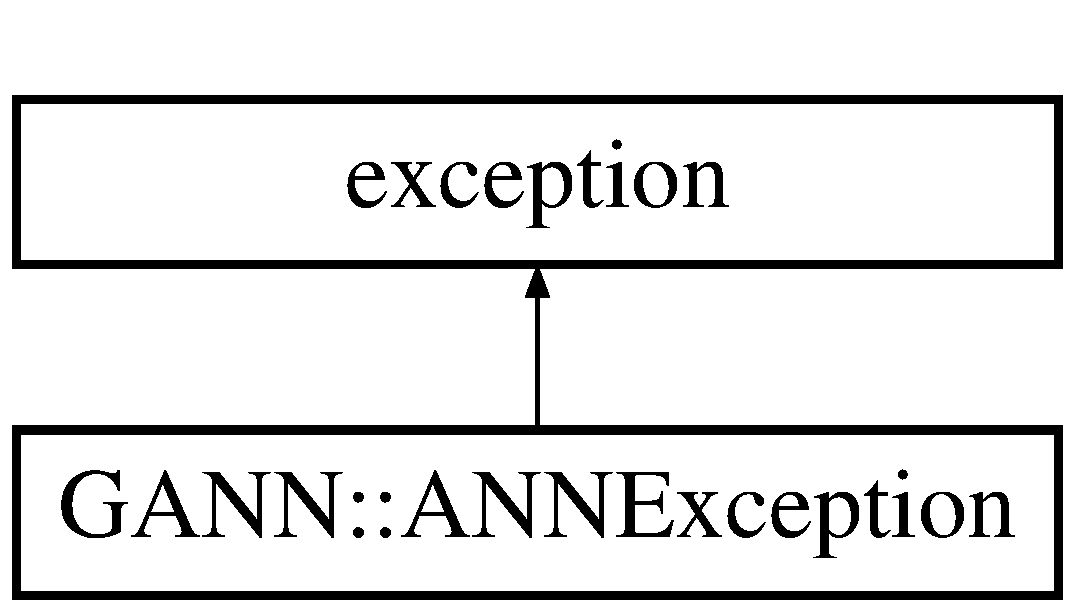
\includegraphics[height=1.944445cm]{class_g_a_n_n_1_1_a_n_n_exception}
\end{center}
\end{figure}
\subsection*{Public Member Functions}
\begin{DoxyCompactItemize}
\item 
{\bfseries A\+N\+N\+Exception} (const char $\ast$message)  throw ()\label{class_g_a_n_n_1_1_a_n_n_exception_ab5cf645781b58f0b3d58c3839012dd4a}

\item 
const char $\ast$ {\bfseries what} (void) const   throw ()\label{class_g_a_n_n_1_1_a_n_n_exception_ac2f2ed402eaf48a7703f845155382d92}

\item 
{\bf A\+N\+N\+Exception} (const char $\ast$message)  throw ()
\begin{DoxyCompactList}\small\item\em Constructor. \end{DoxyCompactList}\item 
{\bf $\sim$\+A\+N\+N\+Exception} (void)  throw ()\label{class_g_a_n_n_1_1_a_n_n_exception_a6332573e3b4b0f08a951fd47de1098aa}

\begin{DoxyCompactList}\small\item\em Destructor. \end{DoxyCompactList}\item 
const char $\ast$ {\bf what} (void) const   throw ()
\begin{DoxyCompactList}\small\item\em Return the error message. \end{DoxyCompactList}\item 
{\bfseries A\+N\+N\+Exception} (const char $\ast$message)  throw ()\label{class_g_a_n_n_1_1_a_n_n_exception_ab5cf645781b58f0b3d58c3839012dd4a}

\item 
const char $\ast$ {\bfseries what} (void) const   throw ()\label{class_g_a_n_n_1_1_a_n_n_exception_a9b16e86cb036634d8520357650c4f201}

\item 
{\bfseries A\+N\+N\+Exception} (const char $\ast$message)  throw ()\label{class_g_a_n_n_1_1_a_n_n_exception_ab5cf645781b58f0b3d58c3839012dd4a}

\item 
const char $\ast$ {\bfseries what} (void) const   throw ()\label{class_g_a_n_n_1_1_a_n_n_exception_a9b16e86cb036634d8520357650c4f201}

\end{DoxyCompactItemize}


\subsection{Detailed Description}
Define the exception that will be used by the \doxyref{G\+A\+N\+N\+::\+A\+N\+N}{p.}{class_g_a_n_n_1_1_a_n_n} class. 

\subsection{Constructor \& Destructor Documentation}
\index{G\+A\+N\+N\+::\+A\+N\+N\+Exception@{G\+A\+N\+N\+::\+A\+N\+N\+Exception}!A\+N\+N\+Exception@{A\+N\+N\+Exception}}
\index{A\+N\+N\+Exception@{A\+N\+N\+Exception}!G\+A\+N\+N\+::\+A\+N\+N\+Exception@{G\+A\+N\+N\+::\+A\+N\+N\+Exception}}
\subsubsection[{A\+N\+N\+Exception(const char $\ast$message)}]{\setlength{\rightskip}{0pt plus 5cm}G\+A\+N\+N\+::\+A\+N\+N\+Exception\+::\+A\+N\+N\+Exception (
\begin{DoxyParamCaption}
\item[{const char $\ast$}]{message}
\end{DoxyParamCaption}
) throw  ) }\label{class_g_a_n_n_1_1_a_n_n_exception_ab5cf645781b58f0b3d58c3839012dd4a}


Constructor. 


\begin{DoxyParams}{Parameters}
{\em message} & \+: Contains the error message. \\
\hline
\end{DoxyParams}


\subsection{Member Function Documentation}
\index{G\+A\+N\+N\+::\+A\+N\+N\+Exception@{G\+A\+N\+N\+::\+A\+N\+N\+Exception}!what@{what}}
\index{what@{what}!G\+A\+N\+N\+::\+A\+N\+N\+Exception@{G\+A\+N\+N\+::\+A\+N\+N\+Exception}}
\subsubsection[{what(void) const }]{\setlength{\rightskip}{0pt plus 5cm}const char$\ast$ G\+A\+N\+N\+::\+A\+N\+N\+Exception\+::what (
\begin{DoxyParamCaption}
\item[{void}]{}
\end{DoxyParamCaption}
) const throw  ) }\label{class_g_a_n_n_1_1_a_n_n_exception_a9b16e86cb036634d8520357650c4f201}


Return the error message. 

\begin{DoxyReturn}{Returns}
const char $\ast$ \+: error message. 
\end{DoxyReturn}


The documentation for this class was generated from the following files\+:\begin{DoxyCompactItemize}
\item 
api/lib/\+A\+N\+N\+Library/include/\+A\+N\+N/ann\+\_\+exception.\+h\item 
api/lib/\+A\+N\+N\+Library/src/\+A\+N\+N/ann\+\_\+exception.\+cc\end{DoxyCompactItemize}

\section{G\+A\+N\+N\+:\+:A\+N\+N\+Layer Class Reference}
\label{class_g_a_n_n_1_1_a_n_n_layer}\index{G\+A\+N\+N\+::\+A\+N\+N\+Layer@{G\+A\+N\+N\+::\+A\+N\+N\+Layer}}


Define a layer of a neural network.  




{\ttfamily \#include $<$ann\+\_\+layer.\+h$>$}

\subsection*{Public Types}
\begin{DoxyCompactItemize}
\item 
typedef double($\ast$ {\bfseries F\+Activate}) (double)\label{class_g_a_n_n_1_1_a_n_n_layer_abb160533dd36e791bd0e561ef244cbae}

\item 
typedef double($\ast$ {\bf F\+Activate}) (double)\label{class_g_a_n_n_1_1_a_n_n_layer_abb160533dd36e791bd0e561ef244cbae}

\begin{DoxyCompactList}\small\item\em Function pointer of an activation function. \end{DoxyCompactList}\item 
typedef double($\ast$ {\bfseries F\+Activate}) (double)\label{class_g_a_n_n_1_1_a_n_n_layer_abb160533dd36e791bd0e561ef244cbae}

\item 
typedef double($\ast$ {\bfseries F\+Activate}) (double)\label{class_g_a_n_n_1_1_a_n_n_layer_abb160533dd36e791bd0e561ef244cbae}

\item 
typedef double($\ast$ {\bfseries F\+Activate}) (double)\label{class_g_a_n_n_1_1_a_n_n_layer_abb160533dd36e791bd0e561ef244cbae}

\end{DoxyCompactItemize}
\subsection*{Public Member Functions}
\begin{DoxyCompactItemize}
\item 
{\bfseries A\+N\+N\+Layer} (unsigned int num\+\_\+inputs, unsigned int num\+\_\+neurons, double min, double max, F\+Activate activation)\label{class_g_a_n_n_1_1_a_n_n_layer_a98a15401495eddad363a75c2ab9c5773}

\item 
{\bfseries A\+N\+N\+Layer} ({\bf A\+N\+N\+Layer} const \&copy)\label{class_g_a_n_n_1_1_a_n_n_layer_a89236bd33096986ab0efa417d4cbcb1c}

\item 
{\bf Matrix}$<$ double $>$ const \& {\bfseries get\+Weights} (void) const \label{class_g_a_n_n_1_1_a_n_n_layer_a53907cae383f48d74ec7377665d99748}

\item 
{\bf Matrix}$<$ double $>$ \& {\bfseries get\+Weights} (void)\label{class_g_a_n_n_1_1_a_n_n_layer_ae91b6f9960dfea801080512dc5d9b224}

\item 
{\bf Matrix}$<$ double $>$ const \& {\bfseries get\+Outputs} (void) const \label{class_g_a_n_n_1_1_a_n_n_layer_a73e68bd212308c07f0e189cac0ce1f78}

\item 
{\bf Matrix}$<$ double $>$ const \& {\bfseries get\+Bias} (void) const \label{class_g_a_n_n_1_1_a_n_n_layer_a667dafc7ab40773bbd6bc32553bd4cb0}

\item 
{\bf Matrix}$<$ double $>$ \& {\bfseries get\+Bias} (void)\label{class_g_a_n_n_1_1_a_n_n_layer_a35de727d75d940dd9614ecdf0f1327ca}

\item 
F\+Activate {\bfseries get\+Activation\+Function} (void) const \label{class_g_a_n_n_1_1_a_n_n_layer_ac6177070fe7bb18aeed82980b70894e1}

\item 
void {\bfseries set\+Weights} ({\bf Matrix}$<$ double $>$ const \&weights)\label{class_g_a_n_n_1_1_a_n_n_layer_a99b44245e660160e6431f4bd8b7cf8ed}

\item 
void {\bfseries set\+Bias} ({\bf Matrix}$<$ double $>$ const \&bias)\label{class_g_a_n_n_1_1_a_n_n_layer_a33b17fa33318cc5ab3060025ccf90faf}

\item 
void {\bfseries set\+Outputs} ({\bf Matrix}$<$ double $>$ const \&outputs)\label{class_g_a_n_n_1_1_a_n_n_layer_a7249be13922695f54aa3ed0b888584b8}

\item 
void {\bfseries set\+Activation\+Function} (F\+Activate f)\label{class_g_a_n_n_1_1_a_n_n_layer_afee60047b0ccb6d2b92f75d4b55febdc}

\item 
{\bf A\+N\+N\+Layer} \& {\bfseries operator=} ({\bf A\+N\+N\+Layer} const \&layer)\label{class_g_a_n_n_1_1_a_n_n_layer_af0143b0bacad70f0fc69969e31f60abb}

\item 
void {\bfseries Activate} ({\bf Matrix}$<$ double $>$ const \&inputs)\label{class_g_a_n_n_1_1_a_n_n_layer_aa8388e643e0916ad8366bb8abc227331}

\item 
{\bf A\+N\+N\+Layer} (unsigned int num\+\_\+inputs, unsigned int num\+\_\+neurons, double min, double max, F\+Activate activation)
\begin{DoxyCompactList}\small\item\em Constructor. \end{DoxyCompactList}\item 
{\bf A\+N\+N\+Layer} ({\bf A\+N\+N\+Layer} const \&copy)
\begin{DoxyCompactList}\small\item\em Constructor. \end{DoxyCompactList}\item 
{\bf A\+N\+N\+Layer} (void)\label{class_g_a_n_n_1_1_a_n_n_layer_a15723dede429598530fefcc7532e9ef8}

\begin{DoxyCompactList}\small\item\em Constructor. \end{DoxyCompactList}\item 
{\bf $\sim$\+A\+N\+N\+Layer} (void)\label{class_g_a_n_n_1_1_a_n_n_layer_a467acde1c266c8f32c2f47764d4e4ee0}

\begin{DoxyCompactList}\small\item\em Destructor. \end{DoxyCompactList}\item 
{\bf Matrix}$<$ double $>$ const \& {\bf get\+Weights} (void) const 
\begin{DoxyCompactList}\small\item\em Get the weights matrix of the neural network. \end{DoxyCompactList}\item 
{\bf Matrix}$<$ double $>$ \& {\bf get\+Weights} (void)
\begin{DoxyCompactList}\small\item\em Get the weights matrix of the neural network. \end{DoxyCompactList}\item 
{\bf Matrix}$<$ double $>$ const \& {\bf get\+Outputs} (void) const \label{class_g_a_n_n_1_1_a_n_n_layer_a47fbef47e9c7c0ef638aed2a2bd30974}

\begin{DoxyCompactList}\small\item\em Get the outputs matrix of the neural network.  G\+A\+N\+N\+::\+Matrix$<$double$>$ const\&. \end{DoxyCompactList}\item 
{\bf Matrix}$<$ double $>$ const \& {\bf get\+Bias} (void) const 
\begin{DoxyCompactList}\small\item\em Get the bias matrix of the neural network. \end{DoxyCompactList}\item 
{\bf Matrix}$<$ double $>$ \& {\bf get\+Bias} (void)
\begin{DoxyCompactList}\small\item\em Get the bias matrix of the neural network. \end{DoxyCompactList}\item 
F\+Activate {\bf get\+Activation\+Function} (void) const 
\begin{DoxyCompactList}\small\item\em Get the activation function of the current layer. \end{DoxyCompactList}\item 
void {\bf set\+Weights} ({\bf Matrix}$<$ double $>$ const \&weights)
\begin{DoxyCompactList}\small\item\em Set the matrix of weights. \end{DoxyCompactList}\item 
void {\bf set\+Bias} ({\bf Matrix}$<$ double $>$ const \&bias)
\begin{DoxyCompactList}\small\item\em Set the matrix of bias. \end{DoxyCompactList}\item 
void {\bf set\+Outputs} ({\bf Matrix}$<$ double $>$ const \&outputs)
\begin{DoxyCompactList}\small\item\em Set the outputs matrix. \end{DoxyCompactList}\item 
void {\bf set\+Activation\+Function} (F\+Activate f)
\begin{DoxyCompactList}\small\item\em Set the activation function of the layer. \end{DoxyCompactList}\item 
{\bf A\+N\+N\+Layer} \& {\bfseries operator=} ({\bf A\+N\+N\+Layer} const \&layer)\label{class_g_a_n_n_1_1_a_n_n_layer_a2b22cd2b08de3d0b41615dd6be0198d4}

\item 
void {\bf Activate} ({\bf Matrix}$<$ double $>$ const \&inputs)
\begin{DoxyCompactList}\small\item\em Activate the current layer and set the matrix of outputs. \end{DoxyCompactList}\item 
{\bfseries A\+N\+N\+Layer} (unsigned int num\+\_\+inputs, unsigned int num\+\_\+neurons, double min, double max, F\+Activate activation)\label{class_g_a_n_n_1_1_a_n_n_layer_a98a15401495eddad363a75c2ab9c5773}

\item 
{\bfseries A\+N\+N\+Layer} ({\bf A\+N\+N\+Layer} const \&copy)\label{class_g_a_n_n_1_1_a_n_n_layer_a89236bd33096986ab0efa417d4cbcb1c}

\item 
{\bf Matrix}$<$ double $>$ const \& {\bfseries get\+Weights} (void) const \label{class_g_a_n_n_1_1_a_n_n_layer_ab2ccaae743a40f1f39595f983db22a8d}

\item 
{\bf Matrix}$<$ double $>$ \& {\bfseries get\+Weights} (void)\label{class_g_a_n_n_1_1_a_n_n_layer_abd06bed4090d09e09669e9ff56b4659a}

\item 
{\bf Matrix}$<$ double $>$ const \& {\bfseries get\+Outputs} (void) const \label{class_g_a_n_n_1_1_a_n_n_layer_a47fbef47e9c7c0ef638aed2a2bd30974}

\item 
{\bf Matrix}$<$ double $>$ const \& {\bfseries get\+Bias} (void) const \label{class_g_a_n_n_1_1_a_n_n_layer_a23a78b0d4255e3480872ba6df6562290}

\item 
{\bf Matrix}$<$ double $>$ \& {\bfseries get\+Bias} (void)\label{class_g_a_n_n_1_1_a_n_n_layer_a2814de885892bd51d23d157fb7ff53a9}

\item 
F\+Activate {\bfseries get\+Activation\+Function} (void) const \label{class_g_a_n_n_1_1_a_n_n_layer_a17a2ecad13a3aac38329470e8575ed62}

\item 
void {\bfseries set\+Weights} ({\bf Matrix}$<$ double $>$ const \&weights)\label{class_g_a_n_n_1_1_a_n_n_layer_a99b44245e660160e6431f4bd8b7cf8ed}

\item 
void {\bfseries set\+Bias} ({\bf Matrix}$<$ double $>$ const \&bias)\label{class_g_a_n_n_1_1_a_n_n_layer_a33b17fa33318cc5ab3060025ccf90faf}

\item 
void {\bfseries set\+Outputs} ({\bf Matrix}$<$ double $>$ const \&outputs)\label{class_g_a_n_n_1_1_a_n_n_layer_a7249be13922695f54aa3ed0b888584b8}

\item 
void {\bfseries set\+Activation\+Function} (F\+Activate f)\label{class_g_a_n_n_1_1_a_n_n_layer_afee60047b0ccb6d2b92f75d4b55febdc}

\item 
{\bf A\+N\+N\+Layer} \& {\bfseries operator=} ({\bf A\+N\+N\+Layer} const \&layer)\label{class_g_a_n_n_1_1_a_n_n_layer_a2b22cd2b08de3d0b41615dd6be0198d4}

\item 
void {\bfseries Activate} ({\bf Matrix}$<$ double $>$ const \&inputs)\label{class_g_a_n_n_1_1_a_n_n_layer_aa8388e643e0916ad8366bb8abc227331}

\item 
{\bfseries A\+N\+N\+Layer} (unsigned int num\+\_\+inputs, unsigned int num\+\_\+neurons, double min, double max, F\+Activate activation)\label{class_g_a_n_n_1_1_a_n_n_layer_a98a15401495eddad363a75c2ab9c5773}

\item 
{\bfseries A\+N\+N\+Layer} ({\bf A\+N\+N\+Layer} const \&copy)\label{class_g_a_n_n_1_1_a_n_n_layer_a89236bd33096986ab0efa417d4cbcb1c}

\item 
{\bf Matrix}$<$ double $>$ const \& {\bfseries get\+Weights} (void) const \label{class_g_a_n_n_1_1_a_n_n_layer_ab2ccaae743a40f1f39595f983db22a8d}

\item 
{\bf Matrix}$<$ double $>$ \& {\bfseries get\+Weights} (void)\label{class_g_a_n_n_1_1_a_n_n_layer_abd06bed4090d09e09669e9ff56b4659a}

\item 
{\bf Matrix}$<$ double $>$ const \& {\bfseries get\+Outputs} (void) const \label{class_g_a_n_n_1_1_a_n_n_layer_a47fbef47e9c7c0ef638aed2a2bd30974}

\item 
{\bf Matrix}$<$ double $>$ const \& {\bfseries get\+Bias} (void) const \label{class_g_a_n_n_1_1_a_n_n_layer_a23a78b0d4255e3480872ba6df6562290}

\item 
{\bf Matrix}$<$ double $>$ \& {\bfseries get\+Bias} (void)\label{class_g_a_n_n_1_1_a_n_n_layer_a2814de885892bd51d23d157fb7ff53a9}

\item 
F\+Activate {\bfseries get\+Activation\+Function} (void) const \label{class_g_a_n_n_1_1_a_n_n_layer_a17a2ecad13a3aac38329470e8575ed62}

\item 
void {\bfseries set\+Weights} ({\bf Matrix}$<$ double $>$ const \&weights)\label{class_g_a_n_n_1_1_a_n_n_layer_a99b44245e660160e6431f4bd8b7cf8ed}

\item 
void {\bfseries set\+Bias} ({\bf Matrix}$<$ double $>$ const \&bias)\label{class_g_a_n_n_1_1_a_n_n_layer_a33b17fa33318cc5ab3060025ccf90faf}

\item 
void {\bfseries set\+Outputs} ({\bf Matrix}$<$ double $>$ const \&outputs)\label{class_g_a_n_n_1_1_a_n_n_layer_a7249be13922695f54aa3ed0b888584b8}

\item 
void {\bfseries set\+Activation\+Function} (F\+Activate f)\label{class_g_a_n_n_1_1_a_n_n_layer_afee60047b0ccb6d2b92f75d4b55febdc}

\item 
{\bf A\+N\+N\+Layer} \& {\bfseries operator=} ({\bf A\+N\+N\+Layer} const \&layer)\label{class_g_a_n_n_1_1_a_n_n_layer_a2b22cd2b08de3d0b41615dd6be0198d4}

\item 
void {\bfseries Activate} ({\bf Matrix}$<$ double $>$ const \&inputs)\label{class_g_a_n_n_1_1_a_n_n_layer_aa8388e643e0916ad8366bb8abc227331}

\item 
{\bfseries A\+N\+N\+Layer} (unsigned int num\+\_\+inputs, unsigned int num\+\_\+neurons, double min, double max, F\+Activate activation)\label{class_g_a_n_n_1_1_a_n_n_layer_a98a15401495eddad363a75c2ab9c5773}

\item 
{\bfseries A\+N\+N\+Layer} ({\bf A\+N\+N\+Layer} const \&copy)\label{class_g_a_n_n_1_1_a_n_n_layer_a89236bd33096986ab0efa417d4cbcb1c}

\item 
{\bf Matrix}$<$ double $>$ const \& {\bfseries get\+Weights} (void) const \label{class_g_a_n_n_1_1_a_n_n_layer_ab2ccaae743a40f1f39595f983db22a8d}

\item 
{\bf Matrix}$<$ double $>$ \& {\bfseries get\+Weights} (void)\label{class_g_a_n_n_1_1_a_n_n_layer_abd06bed4090d09e09669e9ff56b4659a}

\item 
{\bf Matrix}$<$ double $>$ const \& {\bfseries get\+Outputs} (void) const \label{class_g_a_n_n_1_1_a_n_n_layer_a47fbef47e9c7c0ef638aed2a2bd30974}

\item 
{\bf Matrix}$<$ double $>$ const \& {\bfseries get\+Bias} (void) const \label{class_g_a_n_n_1_1_a_n_n_layer_a23a78b0d4255e3480872ba6df6562290}

\item 
{\bf Matrix}$<$ double $>$ \& {\bfseries get\+Bias} (void)\label{class_g_a_n_n_1_1_a_n_n_layer_a2814de885892bd51d23d157fb7ff53a9}

\item 
F\+Activate {\bfseries get\+Activation\+Function} (void) const \label{class_g_a_n_n_1_1_a_n_n_layer_a17a2ecad13a3aac38329470e8575ed62}

\item 
void {\bfseries set\+Weights} ({\bf Matrix}$<$ double $>$ const \&weights)\label{class_g_a_n_n_1_1_a_n_n_layer_a99b44245e660160e6431f4bd8b7cf8ed}

\item 
void {\bfseries set\+Bias} ({\bf Matrix}$<$ double $>$ const \&bias)\label{class_g_a_n_n_1_1_a_n_n_layer_a33b17fa33318cc5ab3060025ccf90faf}

\item 
void {\bfseries set\+Outputs} ({\bf Matrix}$<$ double $>$ const \&outputs)\label{class_g_a_n_n_1_1_a_n_n_layer_a7249be13922695f54aa3ed0b888584b8}

\item 
void {\bfseries set\+Activation\+Function} (F\+Activate f)\label{class_g_a_n_n_1_1_a_n_n_layer_afee60047b0ccb6d2b92f75d4b55febdc}

\item 
{\bf A\+N\+N\+Layer} \& {\bfseries operator=} ({\bf A\+N\+N\+Layer} const \&layer)\label{class_g_a_n_n_1_1_a_n_n_layer_a2b22cd2b08de3d0b41615dd6be0198d4}

\item 
void {\bfseries Activate} ({\bf Matrix}$<$ double $>$ const \&inputs)\label{class_g_a_n_n_1_1_a_n_n_layer_aa8388e643e0916ad8366bb8abc227331}

\end{DoxyCompactItemize}


\subsection{Detailed Description}
Define a layer of a neural network. 

\subsection{Constructor \& Destructor Documentation}
\index{G\+A\+N\+N\+::\+A\+N\+N\+Layer@{G\+A\+N\+N\+::\+A\+N\+N\+Layer}!A\+N\+N\+Layer@{A\+N\+N\+Layer}}
\index{A\+N\+N\+Layer@{A\+N\+N\+Layer}!G\+A\+N\+N\+::\+A\+N\+N\+Layer@{G\+A\+N\+N\+::\+A\+N\+N\+Layer}}
\subsubsection[{A\+N\+N\+Layer(unsigned int num\+\_\+inputs, unsigned int num\+\_\+neurons, double min, double max, F\+Activate activation)}]{\setlength{\rightskip}{0pt plus 5cm}G\+A\+N\+N\+::\+A\+N\+N\+Layer\+::\+A\+N\+N\+Layer (
\begin{DoxyParamCaption}
\item[{unsigned int}]{num\+\_\+inputs, }
\item[{unsigned int}]{num\+\_\+neurons, }
\item[{double}]{min, }
\item[{double}]{max, }
\item[{F\+Activate}]{activation}
\end{DoxyParamCaption}
)}\label{class_g_a_n_n_1_1_a_n_n_layer_a98a15401495eddad363a75c2ab9c5773}


Constructor. 


\begin{DoxyParams}{Parameters}
{\em num\+\_\+inputs} & \+: Contains the number of inputs. \\
\hline
{\em num\+\_\+neurons} & \+: Contains the number of neurons in the layer. \\
\hline
{\em min} & \+: Contains the minimum value of the randomization. \\
\hline
{\em max} & \+: Contains the maximum value of the randomization. \\
\hline
{\em activation} & \+: Contains the function pointer of the activation function. \\
\hline
\end{DoxyParams}
\index{G\+A\+N\+N\+::\+A\+N\+N\+Layer@{G\+A\+N\+N\+::\+A\+N\+N\+Layer}!A\+N\+N\+Layer@{A\+N\+N\+Layer}}
\index{A\+N\+N\+Layer@{A\+N\+N\+Layer}!G\+A\+N\+N\+::\+A\+N\+N\+Layer@{G\+A\+N\+N\+::\+A\+N\+N\+Layer}}
\subsubsection[{A\+N\+N\+Layer(\+A\+N\+N\+Layer const \&copy)}]{\setlength{\rightskip}{0pt plus 5cm}G\+A\+N\+N\+::\+A\+N\+N\+Layer\+::\+A\+N\+N\+Layer (
\begin{DoxyParamCaption}
\item[{{\bf A\+N\+N\+Layer} const \&}]{copy}
\end{DoxyParamCaption}
)}\label{class_g_a_n_n_1_1_a_n_n_layer_a89236bd33096986ab0efa417d4cbcb1c}


Constructor. 


\begin{DoxyParams}{Parameters}
{\em copy} & \+: Contains a layer that will be used in order to create a new layer. \\
\hline
\end{DoxyParams}


\subsection{Member Function Documentation}
\index{G\+A\+N\+N\+::\+A\+N\+N\+Layer@{G\+A\+N\+N\+::\+A\+N\+N\+Layer}!Activate@{Activate}}
\index{Activate@{Activate}!G\+A\+N\+N\+::\+A\+N\+N\+Layer@{G\+A\+N\+N\+::\+A\+N\+N\+Layer}}
\subsubsection[{Activate(\+Matrix$<$ double $>$ const \&inputs)}]{\setlength{\rightskip}{0pt plus 5cm}void G\+A\+N\+N\+::\+A\+N\+N\+Layer\+::\+Activate (
\begin{DoxyParamCaption}
\item[{{\bf Matrix}$<$ double $>$ const \&}]{inputs}
\end{DoxyParamCaption}
)}\label{class_g_a_n_n_1_1_a_n_n_layer_aa8388e643e0916ad8366bb8abc227331}


Activate the current layer and set the matrix of outputs. 


\begin{DoxyParams}{Parameters}
{\em inputs} & \+: Contains the matrix of inputs of the layer. \\
\hline
\end{DoxyParams}
\index{G\+A\+N\+N\+::\+A\+N\+N\+Layer@{G\+A\+N\+N\+::\+A\+N\+N\+Layer}!get\+Activation\+Function@{get\+Activation\+Function}}
\index{get\+Activation\+Function@{get\+Activation\+Function}!G\+A\+N\+N\+::\+A\+N\+N\+Layer@{G\+A\+N\+N\+::\+A\+N\+N\+Layer}}
\subsubsection[{get\+Activation\+Function(void) const }]{\setlength{\rightskip}{0pt plus 5cm}F\+Activate G\+A\+N\+N\+::\+A\+N\+N\+Layer\+::get\+Activation\+Function (
\begin{DoxyParamCaption}
\item[{void}]{}
\end{DoxyParamCaption}
) const}\label{class_g_a_n_n_1_1_a_n_n_layer_a17a2ecad13a3aac38329470e8575ed62}


Get the activation function of the current layer. 

\begin{DoxyReturn}{Returns}
G\+A\+N\+N\+::\+A\+N\+N\+Layer\+::\+F\+Activate 
\end{DoxyReturn}
\index{G\+A\+N\+N\+::\+A\+N\+N\+Layer@{G\+A\+N\+N\+::\+A\+N\+N\+Layer}!get\+Bias@{get\+Bias}}
\index{get\+Bias@{get\+Bias}!G\+A\+N\+N\+::\+A\+N\+N\+Layer@{G\+A\+N\+N\+::\+A\+N\+N\+Layer}}
\subsubsection[{get\+Bias(void) const }]{\setlength{\rightskip}{0pt plus 5cm}{\bf Matrix}$<$double$>$ const\& G\+A\+N\+N\+::\+A\+N\+N\+Layer\+::get\+Bias (
\begin{DoxyParamCaption}
\item[{void}]{}
\end{DoxyParamCaption}
) const}\label{class_g_a_n_n_1_1_a_n_n_layer_a23a78b0d4255e3480872ba6df6562290}


Get the bias matrix of the neural network. 

\begin{DoxyReturn}{Returns}
G\+A\+N\+N\+::\+Matrix$<$double$>$ const\& 
\end{DoxyReturn}
\index{G\+A\+N\+N\+::\+A\+N\+N\+Layer@{G\+A\+N\+N\+::\+A\+N\+N\+Layer}!get\+Bias@{get\+Bias}}
\index{get\+Bias@{get\+Bias}!G\+A\+N\+N\+::\+A\+N\+N\+Layer@{G\+A\+N\+N\+::\+A\+N\+N\+Layer}}
\subsubsection[{get\+Bias(void)}]{\setlength{\rightskip}{0pt plus 5cm}{\bf Matrix}$<$double$>$\& G\+A\+N\+N\+::\+A\+N\+N\+Layer\+::get\+Bias (
\begin{DoxyParamCaption}
\item[{void}]{}
\end{DoxyParamCaption}
)}\label{class_g_a_n_n_1_1_a_n_n_layer_a2814de885892bd51d23d157fb7ff53a9}


Get the bias matrix of the neural network. 

\begin{DoxyReturn}{Returns}
G\+A\+N\+N\+::\+Matrix$<$double$>$ \& 
\end{DoxyReturn}
\index{G\+A\+N\+N\+::\+A\+N\+N\+Layer@{G\+A\+N\+N\+::\+A\+N\+N\+Layer}!get\+Weights@{get\+Weights}}
\index{get\+Weights@{get\+Weights}!G\+A\+N\+N\+::\+A\+N\+N\+Layer@{G\+A\+N\+N\+::\+A\+N\+N\+Layer}}
\subsubsection[{get\+Weights(void) const }]{\setlength{\rightskip}{0pt plus 5cm}{\bf Matrix}$<$double$>$ const\& G\+A\+N\+N\+::\+A\+N\+N\+Layer\+::get\+Weights (
\begin{DoxyParamCaption}
\item[{void}]{}
\end{DoxyParamCaption}
) const}\label{class_g_a_n_n_1_1_a_n_n_layer_ab2ccaae743a40f1f39595f983db22a8d}


Get the weights matrix of the neural network. 

\begin{DoxyReturn}{Returns}
G\+A\+N\+N\+::\+Matrix$<$double$>$ const\& 
\end{DoxyReturn}
\index{G\+A\+N\+N\+::\+A\+N\+N\+Layer@{G\+A\+N\+N\+::\+A\+N\+N\+Layer}!get\+Weights@{get\+Weights}}
\index{get\+Weights@{get\+Weights}!G\+A\+N\+N\+::\+A\+N\+N\+Layer@{G\+A\+N\+N\+::\+A\+N\+N\+Layer}}
\subsubsection[{get\+Weights(void)}]{\setlength{\rightskip}{0pt plus 5cm}{\bf Matrix}$<$double$>$\& G\+A\+N\+N\+::\+A\+N\+N\+Layer\+::get\+Weights (
\begin{DoxyParamCaption}
\item[{void}]{}
\end{DoxyParamCaption}
)}\label{class_g_a_n_n_1_1_a_n_n_layer_abd06bed4090d09e09669e9ff56b4659a}


Get the weights matrix of the neural network. 

\begin{DoxyReturn}{Returns}
G\+A\+N\+N\+::\+Matrix$<$double$>$ \& 
\end{DoxyReturn}
\index{G\+A\+N\+N\+::\+A\+N\+N\+Layer@{G\+A\+N\+N\+::\+A\+N\+N\+Layer}!set\+Activation\+Function@{set\+Activation\+Function}}
\index{set\+Activation\+Function@{set\+Activation\+Function}!G\+A\+N\+N\+::\+A\+N\+N\+Layer@{G\+A\+N\+N\+::\+A\+N\+N\+Layer}}
\subsubsection[{set\+Activation\+Function(\+F\+Activate f)}]{\setlength{\rightskip}{0pt plus 5cm}void G\+A\+N\+N\+::\+A\+N\+N\+Layer\+::set\+Activation\+Function (
\begin{DoxyParamCaption}
\item[{F\+Activate}]{f}
\end{DoxyParamCaption}
)}\label{class_g_a_n_n_1_1_a_n_n_layer_afee60047b0ccb6d2b92f75d4b55febdc}


Set the activation function of the layer. 


\begin{DoxyParams}{Parameters}
{\em f} & \+: Contains the function pointer of the activation function. \\
\hline
\end{DoxyParams}
\index{G\+A\+N\+N\+::\+A\+N\+N\+Layer@{G\+A\+N\+N\+::\+A\+N\+N\+Layer}!set\+Bias@{set\+Bias}}
\index{set\+Bias@{set\+Bias}!G\+A\+N\+N\+::\+A\+N\+N\+Layer@{G\+A\+N\+N\+::\+A\+N\+N\+Layer}}
\subsubsection[{set\+Bias(\+Matrix$<$ double $>$ const \&bias)}]{\setlength{\rightskip}{0pt plus 5cm}void G\+A\+N\+N\+::\+A\+N\+N\+Layer\+::set\+Bias (
\begin{DoxyParamCaption}
\item[{{\bf Matrix}$<$ double $>$ const \&}]{bias}
\end{DoxyParamCaption}
)}\label{class_g_a_n_n_1_1_a_n_n_layer_a33b17fa33318cc5ab3060025ccf90faf}


Set the matrix of bias. 


\begin{DoxyParams}{Parameters}
{\em bias} & \+: Contains the matrix of bias. \\
\hline
\end{DoxyParams}
\index{G\+A\+N\+N\+::\+A\+N\+N\+Layer@{G\+A\+N\+N\+::\+A\+N\+N\+Layer}!set\+Outputs@{set\+Outputs}}
\index{set\+Outputs@{set\+Outputs}!G\+A\+N\+N\+::\+A\+N\+N\+Layer@{G\+A\+N\+N\+::\+A\+N\+N\+Layer}}
\subsubsection[{set\+Outputs(\+Matrix$<$ double $>$ const \&outputs)}]{\setlength{\rightskip}{0pt plus 5cm}void G\+A\+N\+N\+::\+A\+N\+N\+Layer\+::set\+Outputs (
\begin{DoxyParamCaption}
\item[{{\bf Matrix}$<$ double $>$ const \&}]{outputs}
\end{DoxyParamCaption}
)}\label{class_g_a_n_n_1_1_a_n_n_layer_a7249be13922695f54aa3ed0b888584b8}


Set the outputs matrix. 


\begin{DoxyParams}{Parameters}
{\em outputs} & \+: Contains the matrix of outputs.\+x \\
\hline
\end{DoxyParams}
\index{G\+A\+N\+N\+::\+A\+N\+N\+Layer@{G\+A\+N\+N\+::\+A\+N\+N\+Layer}!set\+Weights@{set\+Weights}}
\index{set\+Weights@{set\+Weights}!G\+A\+N\+N\+::\+A\+N\+N\+Layer@{G\+A\+N\+N\+::\+A\+N\+N\+Layer}}
\subsubsection[{set\+Weights(\+Matrix$<$ double $>$ const \&weights)}]{\setlength{\rightskip}{0pt plus 5cm}void G\+A\+N\+N\+::\+A\+N\+N\+Layer\+::set\+Weights (
\begin{DoxyParamCaption}
\item[{{\bf Matrix}$<$ double $>$ const \&}]{weights}
\end{DoxyParamCaption}
)}\label{class_g_a_n_n_1_1_a_n_n_layer_a99b44245e660160e6431f4bd8b7cf8ed}


Set the matrix of weights. 


\begin{DoxyParams}{Parameters}
{\em weights} & \+: Contains the matrix of weights. \\
\hline
\end{DoxyParams}


The documentation for this class was generated from the following files\+:\begin{DoxyCompactItemize}
\item 
api/lib/\+A\+N\+N\+Library/include/\+A\+N\+N/ann\+\_\+layer.\+h\item 
api/lib/\+A\+N\+N\+Library/src/\+A\+N\+N/ann\+\_\+layer.\+cc\end{DoxyCompactItemize}

\section{Json\+:\+:Built\+Styled\+Stream\+Writer Struct Reference}
\label{struct_json_1_1_built_styled_stream_writer}\index{Json\+::\+Built\+Styled\+Stream\+Writer@{Json\+::\+Built\+Styled\+Stream\+Writer}}
Inheritance diagram for Json\+:\+:Built\+Styled\+Stream\+Writer\+:\begin{figure}[H]
\begin{center}
\leavevmode
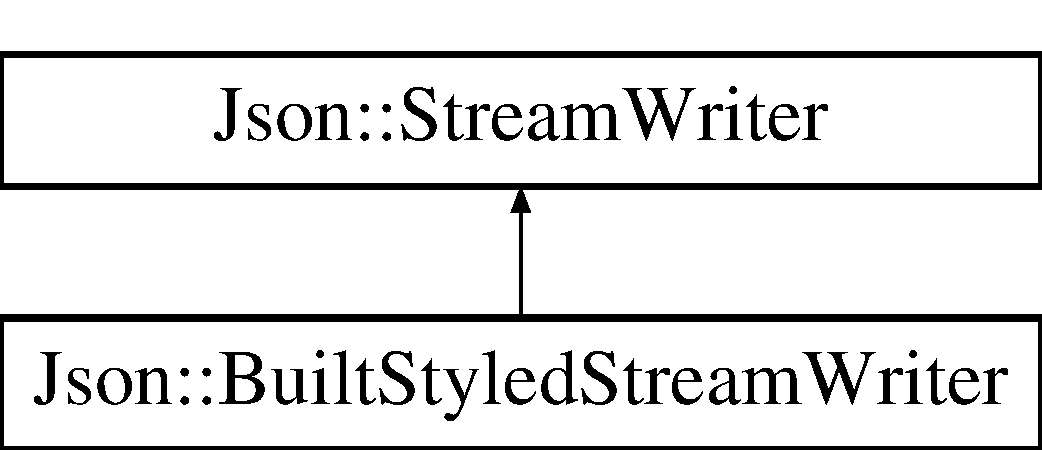
\includegraphics[height=2.000000cm]{struct_json_1_1_built_styled_stream_writer}
\end{center}
\end{figure}
\subsection*{Public Member Functions}
\begin{DoxyCompactItemize}
\item 
{\bfseries Built\+Styled\+Stream\+Writer} (std\+::string const \&indentation, {\bf Comment\+Style\+::\+Enum} cs, std\+::string const \&colon\+Symbol, std\+::string const \&null\+Symbol, std\+::string const \&ending\+Line\+Feed\+Symbol)\label{struct_json_1_1_built_styled_stream_writer_a3c5c0a88ff6b04e1e94a001f82544c65}

\item 
virtual int {\bf write} ({\bf Value} const \&root, std\+::ostream $\ast$sout)
\item 
{\bfseries Built\+Styled\+Stream\+Writer} (std\+::string const \&indentation, {\bf Comment\+Style\+::\+Enum} cs, std\+::string const \&colon\+Symbol, std\+::string const \&null\+Symbol, std\+::string const \&ending\+Line\+Feed\+Symbol)\label{struct_json_1_1_built_styled_stream_writer_a3c5c0a88ff6b04e1e94a001f82544c65}

\item 
virtual int {\bf write} ({\bf Value} const \&root, std\+::ostream $\ast$sout)
\item 
{\bfseries Built\+Styled\+Stream\+Writer} (std\+::string const \&indentation, {\bf Comment\+Style\+::\+Enum} cs, std\+::string const \&colon\+Symbol, std\+::string const \&null\+Symbol, std\+::string const \&ending\+Line\+Feed\+Symbol)\label{struct_json_1_1_built_styled_stream_writer_a3c5c0a88ff6b04e1e94a001f82544c65}

\item 
virtual int {\bf write} ({\bf Value} const \&root, std\+::ostream $\ast$sout)
\end{DoxyCompactItemize}
\subsection*{Additional Inherited Members}


\subsection{Member Function Documentation}
\index{Json\+::\+Built\+Styled\+Stream\+Writer@{Json\+::\+Built\+Styled\+Stream\+Writer}!write@{write}}
\index{write@{write}!Json\+::\+Built\+Styled\+Stream\+Writer@{Json\+::\+Built\+Styled\+Stream\+Writer}}
\subsubsection[{write(\+Value const \&root, std\+::ostream $\ast$sout)}]{\setlength{\rightskip}{0pt plus 5cm}int Json\+::\+Built\+Styled\+Stream\+Writer\+::write (
\begin{DoxyParamCaption}
\item[{{\bf Value} const \&}]{root, }
\item[{std\+::ostream $\ast$}]{sout}
\end{DoxyParamCaption}
)\hspace{0.3cm}{\ttfamily [virtual]}}\label{struct_json_1_1_built_styled_stream_writer_ab8810d938c35c8442cbffcd001628cd0}
Write \doxyref{Value}{p.}{class_json_1_1_value} into document as configured in sub-\/class. Do not take ownership of sout, but maintain a reference during function. \begin{DoxyPrecond}{Precondition}
sout != N\+U\+L\+L 
\end{DoxyPrecond}
\begin{DoxyReturn}{Returns}
zero on success (For now, we always return zero, so check the stream instead.) 
\end{DoxyReturn}

\begin{DoxyExceptions}{Exceptions}
{\em std\+::exception} & possibly, depending on configuration \\
\hline
\end{DoxyExceptions}


Implements {\bf Json\+::\+Stream\+Writer} \doxyref{}{p.}{class_json_1_1_stream_writer_a237368cf13b41decc015640d25f176ab}.

\index{Json\+::\+Built\+Styled\+Stream\+Writer@{Json\+::\+Built\+Styled\+Stream\+Writer}!write@{write}}
\index{write@{write}!Json\+::\+Built\+Styled\+Stream\+Writer@{Json\+::\+Built\+Styled\+Stream\+Writer}}
\subsubsection[{write(\+Value const \&root, std\+::ostream $\ast$sout)}]{\setlength{\rightskip}{0pt plus 5cm}virtual int Json\+::\+Built\+Styled\+Stream\+Writer\+::write (
\begin{DoxyParamCaption}
\item[{{\bf Value} const \&}]{root, }
\item[{std\+::ostream $\ast$}]{sout}
\end{DoxyParamCaption}
)\hspace{0.3cm}{\ttfamily [virtual]}}\label{struct_json_1_1_built_styled_stream_writer_af3af7e55185c8c0d503f6cf9baa2f844}
Write \doxyref{Value}{p.}{class_json_1_1_value} into document as configured in sub-\/class. Do not take ownership of sout, but maintain a reference during function. \begin{DoxyPrecond}{Precondition}
sout != N\+U\+L\+L 
\end{DoxyPrecond}
\begin{DoxyReturn}{Returns}
zero on success (For now, we always return zero, so check the stream instead.) 
\end{DoxyReturn}

\begin{DoxyExceptions}{Exceptions}
{\em std\+::exception} & possibly, depending on configuration \\
\hline
\end{DoxyExceptions}


Implements {\bf Json\+::\+Stream\+Writer} \doxyref{}{p.}{class_json_1_1_stream_writer_a237368cf13b41decc015640d25f176ab}.

\index{Json\+::\+Built\+Styled\+Stream\+Writer@{Json\+::\+Built\+Styled\+Stream\+Writer}!write@{write}}
\index{write@{write}!Json\+::\+Built\+Styled\+Stream\+Writer@{Json\+::\+Built\+Styled\+Stream\+Writer}}
\subsubsection[{write(\+Value const \&root, std\+::ostream $\ast$sout)}]{\setlength{\rightskip}{0pt plus 5cm}virtual int Json\+::\+Built\+Styled\+Stream\+Writer\+::write (
\begin{DoxyParamCaption}
\item[{{\bf Value} const \&}]{root, }
\item[{std\+::ostream $\ast$}]{sout}
\end{DoxyParamCaption}
)\hspace{0.3cm}{\ttfamily [virtual]}}\label{struct_json_1_1_built_styled_stream_writer_af3af7e55185c8c0d503f6cf9baa2f844}
Write \doxyref{Value}{p.}{class_json_1_1_value} into document as configured in sub-\/class. Do not take ownership of sout, but maintain a reference during function. \begin{DoxyPrecond}{Precondition}
sout != N\+U\+L\+L 
\end{DoxyPrecond}
\begin{DoxyReturn}{Returns}
zero on success (For now, we always return zero, so check the stream instead.) 
\end{DoxyReturn}

\begin{DoxyExceptions}{Exceptions}
{\em std\+::exception} & possibly, depending on configuration \\
\hline
\end{DoxyExceptions}


Implements {\bf Json\+::\+Stream\+Writer} \doxyref{}{p.}{class_json_1_1_stream_writer_a237368cf13b41decc015640d25f176ab}.



The documentation for this struct was generated from the following file\+:\begin{DoxyCompactItemize}
\item 
/home/robin\+\_\+f/\+Programming/\+Git/\+C\+P\+P/\+Love\+Brains/api/lib/\+A\+N\+N\+Library/src/json/jsoncpp.\+cc\end{DoxyCompactItemize}

\hypertarget{class_json_1_1_char_reader}{}\section{Json\+:\+:Char\+Reader Class Reference}
\label{class_json_1_1_char_reader}\index{Json\+::\+Char\+Reader@{Json\+::\+Char\+Reader}}


{\ttfamily \#include $<$json.\+h$>$}

Inheritance diagram for Json\+:\+:Char\+Reader\+:\begin{figure}[H]
\begin{center}
\leavevmode
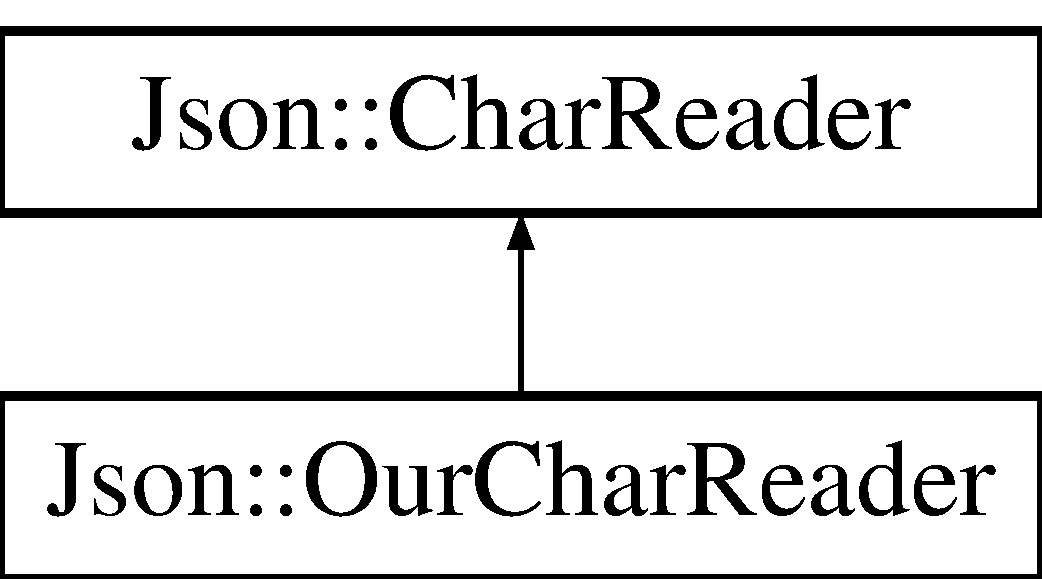
\includegraphics[height=2.000000cm]{class_json_1_1_char_reader}
\end{center}
\end{figure}
\subsection*{Classes}
\begin{DoxyCompactItemize}
\item 
class \hyperlink{class_json_1_1_char_reader_1_1_factory}{Factory}
\end{DoxyCompactItemize}
\subsection*{Public Member Functions}
\begin{DoxyCompactItemize}
\item 
virtual bool \hyperlink{class_json_1_1_char_reader_a48e320be8b13bbc0960cc5808cafec98}{parse} (char const $\ast$begin\+Doc, char const $\ast$end\+Doc, \hyperlink{class_json_1_1_value}{Value} $\ast$root, std\+::string $\ast$errs)=0
\begin{DoxyCompactList}\small\item\em Read a \hyperlink{class_json_1_1_value}{Value} from a \href{http://www.json.org}{\tt J\+S\+O\+N} document. The document must be a U\+T\+F-\/8 encoded string containing the document to read. \end{DoxyCompactList}\end{DoxyCompactItemize}


\subsection{Detailed Description}
Interface for reading J\+S\+O\+N from a char array. 

\subsection{Member Function Documentation}
\hypertarget{class_json_1_1_char_reader_a48e320be8b13bbc0960cc5808cafec98}{}\index{Json\+::\+Char\+Reader@{Json\+::\+Char\+Reader}!parse@{parse}}
\index{parse@{parse}!Json\+::\+Char\+Reader@{Json\+::\+Char\+Reader}}
\subsubsection[{parse(char const $\ast$begin\+Doc, char const $\ast$end\+Doc, Value $\ast$root, std\+::string $\ast$errs)=0}]{\setlength{\rightskip}{0pt plus 5cm}virtual bool Json\+::\+Char\+Reader\+::parse (
\begin{DoxyParamCaption}
\item[{char const $\ast$}]{begin\+Doc, }
\item[{char const $\ast$}]{end\+Doc, }
\item[{{\bf Value} $\ast$}]{root, }
\item[{std\+::string $\ast$}]{errs}
\end{DoxyParamCaption}
)\hspace{0.3cm}{\ttfamily [pure virtual]}}\label{class_json_1_1_char_reader_a48e320be8b13bbc0960cc5808cafec98}


Read a \hyperlink{class_json_1_1_value}{Value} from a \href{http://www.json.org}{\tt J\+S\+O\+N} document. The document must be a U\+T\+F-\/8 encoded string containing the document to read. 


\begin{DoxyParams}{Parameters}
{\em begin\+Doc} & Pointer on the beginning of the U\+T\+F-\/8 encoded string of the document to read. \\
\hline
{\em end\+Doc} & Pointer on the end of the U\+T\+F-\/8 encoded string of the document to read. Must be $>$= begin\+Doc. \\
\hline
{\em root} & \mbox{[}out\mbox{]} Contains the root value of the document if it was successfully parsed. \\
\hline
{\em errs} & \mbox{[}out\mbox{]} Formatted error messages (if not N\+U\+L\+L) a user friendly string that lists errors in the parsed document. \\
\hline
\end{DoxyParams}
\begin{DoxyReturn}{Returns}
{\ttfamily true} if the document was successfully parsed, {\ttfamily false} if an error occurred. 
\end{DoxyReturn}


Implemented in \hyperlink{class_json_1_1_our_char_reader_aa4dce03aee1c111679813133c29f4465}{Json\+::\+Our\+Char\+Reader}.



The documentation for this class was generated from the following file\+:\begin{DoxyCompactItemize}
\item 
/home/robin\+\_\+f/\+Programming/\+Git/\+C\+P\+P/\+Love\+Brains/api/lib/\+A\+N\+N\+Library/include/json/json.\+h\end{DoxyCompactItemize}

\section{Json\+:\+:Char\+Reader\+Builder Class Reference}
\label{class_json_1_1_char_reader_builder}\index{Json\+::\+Char\+Reader\+Builder@{Json\+::\+Char\+Reader\+Builder}}


Build a \doxyref{Char\+Reader}{p.}{class_json_1_1_char_reader} implementation.  




{\ttfamily \#include $<$json.\+h$>$}

Inheritance diagram for Json\+:\+:Char\+Reader\+Builder\+:\begin{figure}[H]
\begin{center}
\leavevmode
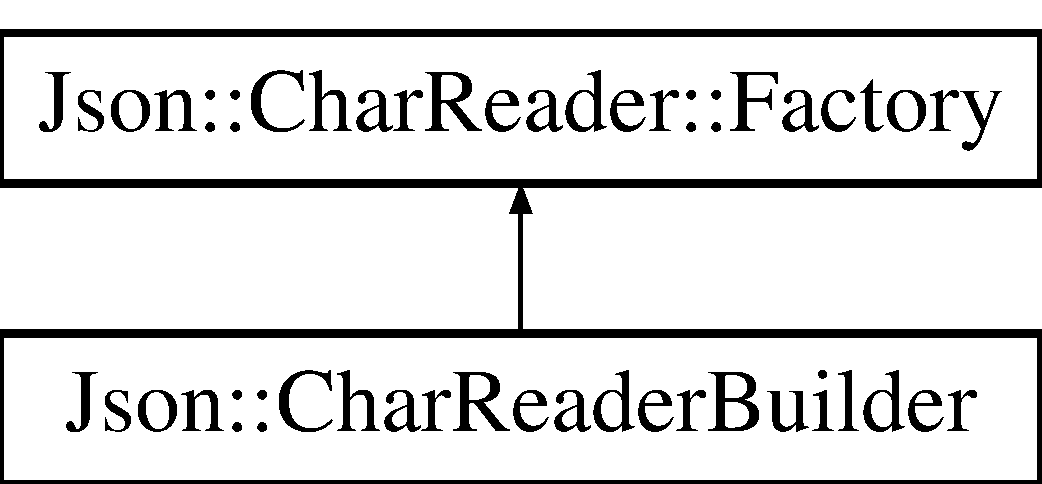
\includegraphics[height=1.627907cm]{class_json_1_1_char_reader_builder}
\end{center}
\end{figure}
\subsection*{Public Member Functions}
\begin{DoxyCompactItemize}
\item 
virtual {\bf Char\+Reader} $\ast$ {\bf new\+Char\+Reader} () const 
\begin{DoxyCompactList}\small\item\em Allocate a \doxyref{Char\+Reader}{p.}{class_json_1_1_char_reader} via operator new(). \end{DoxyCompactList}\item 
bool {\bf validate} ({\bf Json\+::\+Value} $\ast$invalid) const 
\item 
{\bf Value} \& {\bf operator[$\,$]} (std\+::string key)
\item 
virtual {\bf Char\+Reader} $\ast$ {\bf new\+Char\+Reader} () const 
\begin{DoxyCompactList}\small\item\em Allocate a \doxyref{Char\+Reader}{p.}{class_json_1_1_char_reader} via operator new(). \end{DoxyCompactList}\item 
bool {\bf validate} ({\bf Json\+::\+Value} $\ast$invalid) const 
\item 
{\bf Value} \& {\bf operator[$\,$]} (std\+::string key)
\item 
virtual {\bf Char\+Reader} $\ast$ {\bf new\+Char\+Reader} () const 
\begin{DoxyCompactList}\small\item\em Allocate a \doxyref{Char\+Reader}{p.}{class_json_1_1_char_reader} via operator new(). \end{DoxyCompactList}\item 
bool {\bf validate} ({\bf Json\+::\+Value} $\ast$invalid) const 
\item 
{\bf Value} \& {\bf operator[$\,$]} (std\+::string key)
\item 
virtual {\bf Char\+Reader} $\ast$ {\bf new\+Char\+Reader} () const 
\begin{DoxyCompactList}\small\item\em Allocate a \doxyref{Char\+Reader}{p.}{class_json_1_1_char_reader} via operator new(). \end{DoxyCompactList}\item 
bool {\bf validate} ({\bf Json\+::\+Value} $\ast$invalid) const 
\item 
{\bf Value} \& {\bf operator[$\,$]} (std\+::string key)
\end{DoxyCompactItemize}
\subsection*{Static Public Member Functions}
\begin{DoxyCompactItemize}
\item 
static void {\bf set\+Defaults} ({\bf Json\+::\+Value} $\ast$settings)
\item 
static void {\bf strict\+Mode} ({\bf Json\+::\+Value} $\ast$settings)
\item 
static void {\bf set\+Defaults} ({\bf Json\+::\+Value} $\ast$settings)
\item 
static void {\bf strict\+Mode} ({\bf Json\+::\+Value} $\ast$settings)
\item 
static void {\bf set\+Defaults} ({\bf Json\+::\+Value} $\ast$settings)
\item 
static void {\bf strict\+Mode} ({\bf Json\+::\+Value} $\ast$settings)
\item 
static void {\bf set\+Defaults} ({\bf Json\+::\+Value} $\ast$settings)
\item 
static void {\bf strict\+Mode} ({\bf Json\+::\+Value} $\ast$settings)
\end{DoxyCompactItemize}
\subsection*{Public Attributes}
\begin{DoxyCompactItemize}
\item 
{\bf Json\+::\+Value} {\bf settings\+\_\+}
\end{DoxyCompactItemize}


\subsection{Detailed Description}
Build a \doxyref{Char\+Reader}{p.}{class_json_1_1_char_reader} implementation. 

Usage\+: 
\begin{DoxyCode}
\textcolor{keyword}{using namespace }Json;
CharReaderBuilder builder;
builder[\textcolor{stringliteral}{"collectComments"}] = \textcolor{keyword}{false};
Value value;
std::string errs;
\textcolor{keywordtype}{bool} ok = parseFromStream(builder, std::cin, &value, &errs);
\end{DoxyCode}
 

\subsection{Member Function Documentation}
\index{Json\+::\+Char\+Reader\+Builder@{Json\+::\+Char\+Reader\+Builder}!new\+Char\+Reader@{new\+Char\+Reader}}
\index{new\+Char\+Reader@{new\+Char\+Reader}!Json\+::\+Char\+Reader\+Builder@{Json\+::\+Char\+Reader\+Builder}}
\subsubsection[{new\+Char\+Reader() const }]{\setlength{\rightskip}{0pt plus 5cm}{\bf Char\+Reader} $\ast$ Json\+::\+Char\+Reader\+Builder\+::new\+Char\+Reader (
\begin{DoxyParamCaption}
{}
\end{DoxyParamCaption}
) const\hspace{0.3cm}{\ttfamily [virtual]}}\label{class_json_1_1_char_reader_builder_a3e3c9f4aeb07023ef0c5f6255003078a}


Allocate a \doxyref{Char\+Reader}{p.}{class_json_1_1_char_reader} via operator new(). 


\begin{DoxyExceptions}{Exceptions}
{\em std\+::exception} & if something goes wrong (e.\+g. invalid settings) \\
\hline
\end{DoxyExceptions}


Implements {\bf Json\+::\+Char\+Reader\+::\+Factory} \doxyref{}{p.}{class_json_1_1_char_reader_1_1_factory_a497112c51f36a676aeb496c3a91d38d0}.

\index{Json\+::\+Char\+Reader\+Builder@{Json\+::\+Char\+Reader\+Builder}!new\+Char\+Reader@{new\+Char\+Reader}}
\index{new\+Char\+Reader@{new\+Char\+Reader}!Json\+::\+Char\+Reader\+Builder@{Json\+::\+Char\+Reader\+Builder}}
\subsubsection[{new\+Char\+Reader() const }]{\setlength{\rightskip}{0pt plus 5cm}virtual {\bf Char\+Reader}$\ast$ Json\+::\+Char\+Reader\+Builder\+::new\+Char\+Reader (
\begin{DoxyParamCaption}
{}
\end{DoxyParamCaption}
) const\hspace{0.3cm}{\ttfamily [virtual]}}\label{class_json_1_1_char_reader_builder_a7154f2d99e35596b98c743feb643ebe4}


Allocate a \doxyref{Char\+Reader}{p.}{class_json_1_1_char_reader} via operator new(). 


\begin{DoxyExceptions}{Exceptions}
{\em std\+::exception} & if something goes wrong (e.\+g. invalid settings) \\
\hline
\end{DoxyExceptions}


Implements {\bf Json\+::\+Char\+Reader\+::\+Factory} \doxyref{}{p.}{class_json_1_1_char_reader_1_1_factory_a497112c51f36a676aeb496c3a91d38d0}.

\index{Json\+::\+Char\+Reader\+Builder@{Json\+::\+Char\+Reader\+Builder}!new\+Char\+Reader@{new\+Char\+Reader}}
\index{new\+Char\+Reader@{new\+Char\+Reader}!Json\+::\+Char\+Reader\+Builder@{Json\+::\+Char\+Reader\+Builder}}
\subsubsection[{new\+Char\+Reader() const }]{\setlength{\rightskip}{0pt plus 5cm}virtual {\bf Char\+Reader}$\ast$ Json\+::\+Char\+Reader\+Builder\+::new\+Char\+Reader (
\begin{DoxyParamCaption}
{}
\end{DoxyParamCaption}
) const\hspace{0.3cm}{\ttfamily [virtual]}}\label{class_json_1_1_char_reader_builder_a7154f2d99e35596b98c743feb643ebe4}


Allocate a \doxyref{Char\+Reader}{p.}{class_json_1_1_char_reader} via operator new(). 


\begin{DoxyExceptions}{Exceptions}
{\em std\+::exception} & if something goes wrong (e.\+g. invalid settings) \\
\hline
\end{DoxyExceptions}


Implements {\bf Json\+::\+Char\+Reader\+::\+Factory} \doxyref{}{p.}{class_json_1_1_char_reader_1_1_factory_a497112c51f36a676aeb496c3a91d38d0}.

\index{Json\+::\+Char\+Reader\+Builder@{Json\+::\+Char\+Reader\+Builder}!new\+Char\+Reader@{new\+Char\+Reader}}
\index{new\+Char\+Reader@{new\+Char\+Reader}!Json\+::\+Char\+Reader\+Builder@{Json\+::\+Char\+Reader\+Builder}}
\subsubsection[{new\+Char\+Reader() const }]{\setlength{\rightskip}{0pt plus 5cm}virtual {\bf Char\+Reader}$\ast$ Json\+::\+Char\+Reader\+Builder\+::new\+Char\+Reader (
\begin{DoxyParamCaption}
{}
\end{DoxyParamCaption}
) const\hspace{0.3cm}{\ttfamily [virtual]}}\label{class_json_1_1_char_reader_builder_a7154f2d99e35596b98c743feb643ebe4}


Allocate a \doxyref{Char\+Reader}{p.}{class_json_1_1_char_reader} via operator new(). 


\begin{DoxyExceptions}{Exceptions}
{\em std\+::exception} & if something goes wrong (e.\+g. invalid settings) \\
\hline
\end{DoxyExceptions}


Implements {\bf Json\+::\+Char\+Reader\+::\+Factory} \doxyref{}{p.}{class_json_1_1_char_reader_1_1_factory_a497112c51f36a676aeb496c3a91d38d0}.

\index{Json\+::\+Char\+Reader\+Builder@{Json\+::\+Char\+Reader\+Builder}!operator[$\,$]@{operator[]}}
\index{operator[$\,$]@{operator[]}!Json\+::\+Char\+Reader\+Builder@{Json\+::\+Char\+Reader\+Builder}}
\subsubsection[{operator[](std\+::string key)}]{\setlength{\rightskip}{0pt plus 5cm}{\bf Value}\& Json\+::\+Char\+Reader\+Builder\+::operator[$\,$] (
\begin{DoxyParamCaption}
\item[{std\+::string}]{key}
\end{DoxyParamCaption}
)}\label{class_json_1_1_char_reader_builder_a4325482962145ef8d7c0e7672002cb26}
A simple way to update a specific setting. \index{Json\+::\+Char\+Reader\+Builder@{Json\+::\+Char\+Reader\+Builder}!operator[$\,$]@{operator[]}}
\index{operator[$\,$]@{operator[]}!Json\+::\+Char\+Reader\+Builder@{Json\+::\+Char\+Reader\+Builder}}
\subsubsection[{operator[](std\+::string key)}]{\setlength{\rightskip}{0pt plus 5cm}{\bf Value}\& Json\+::\+Char\+Reader\+Builder\+::operator[$\,$] (
\begin{DoxyParamCaption}
\item[{std\+::string}]{key}
\end{DoxyParamCaption}
)}\label{class_json_1_1_char_reader_builder_a4325482962145ef8d7c0e7672002cb26}
A simple way to update a specific setting. \index{Json\+::\+Char\+Reader\+Builder@{Json\+::\+Char\+Reader\+Builder}!operator[$\,$]@{operator[]}}
\index{operator[$\,$]@{operator[]}!Json\+::\+Char\+Reader\+Builder@{Json\+::\+Char\+Reader\+Builder}}
\subsubsection[{operator[](std\+::string key)}]{\setlength{\rightskip}{0pt plus 5cm}{\bf Value} \& Json\+::\+Char\+Reader\+Builder\+::operator[$\,$] (
\begin{DoxyParamCaption}
\item[{std\+::string}]{key}
\end{DoxyParamCaption}
)}\label{class_json_1_1_char_reader_builder_a324561448113b48eb7aa6e6a5ce3aa0d}
A simple way to update a specific setting. \index{Json\+::\+Char\+Reader\+Builder@{Json\+::\+Char\+Reader\+Builder}!operator[$\,$]@{operator[]}}
\index{operator[$\,$]@{operator[]}!Json\+::\+Char\+Reader\+Builder@{Json\+::\+Char\+Reader\+Builder}}
\subsubsection[{operator[](std\+::string key)}]{\setlength{\rightskip}{0pt plus 5cm}{\bf Value}\& Json\+::\+Char\+Reader\+Builder\+::operator[$\,$] (
\begin{DoxyParamCaption}
\item[{std\+::string}]{key}
\end{DoxyParamCaption}
)}\label{class_json_1_1_char_reader_builder_a4325482962145ef8d7c0e7672002cb26}
A simple way to update a specific setting. \index{Json\+::\+Char\+Reader\+Builder@{Json\+::\+Char\+Reader\+Builder}!set\+Defaults@{set\+Defaults}}
\index{set\+Defaults@{set\+Defaults}!Json\+::\+Char\+Reader\+Builder@{Json\+::\+Char\+Reader\+Builder}}
\subsubsection[{set\+Defaults(\+Json\+::\+Value $\ast$settings)}]{\setlength{\rightskip}{0pt plus 5cm}static void Json\+::\+Char\+Reader\+Builder\+::set\+Defaults (
\begin{DoxyParamCaption}
\item[{{\bf Json\+::\+Value} $\ast$}]{settings}
\end{DoxyParamCaption}
)\hspace{0.3cm}{\ttfamily [static]}}\label{class_json_1_1_char_reader_builder_a0ddbea7a0af6da9feea922fbe4e5d6c6}
Called by ctor, but you can use this to reset settings\+\_\+. \begin{DoxyPrecond}{Precondition}
\textquotesingle{}settings\textquotesingle{} != N\+U\+L\+L (but Json\+::null is fine) 
\end{DoxyPrecond}
\begin{DoxyRemark}{Remarks}
Defaults\+: 
\begin{DoxyCodeInclude}
\end{DoxyCodeInclude}

\end{DoxyRemark}
\index{Json\+::\+Char\+Reader\+Builder@{Json\+::\+Char\+Reader\+Builder}!set\+Defaults@{set\+Defaults}}
\index{set\+Defaults@{set\+Defaults}!Json\+::\+Char\+Reader\+Builder@{Json\+::\+Char\+Reader\+Builder}}
\subsubsection[{set\+Defaults(\+Json\+::\+Value $\ast$settings)}]{\setlength{\rightskip}{0pt plus 5cm}void Json\+::\+Char\+Reader\+Builder\+::set\+Defaults (
\begin{DoxyParamCaption}
\item[{{\bf Json\+::\+Value} $\ast$}]{settings}
\end{DoxyParamCaption}
)\hspace{0.3cm}{\ttfamily [static]}}\label{class_json_1_1_char_reader_builder_a03ff031e06aabff989ab4addc87294ab}
Called by ctor, but you can use this to reset settings\+\_\+. \begin{DoxyPrecond}{Precondition}
\textquotesingle{}settings\textquotesingle{} != N\+U\+L\+L (but Json\+::null is fine) 
\end{DoxyPrecond}
\begin{DoxyRemark}{Remarks}
Defaults\+: 
\begin{DoxyCodeInclude}
\end{DoxyCodeInclude}

\end{DoxyRemark}
[Char\+Reader\+Builder\+Defaults]

[Char\+Reader\+Builder\+Defaults]

[Char\+Reader\+Builder\+Defaults]

[Char\+Reader\+Builder\+Defaults]

[Char\+Reader\+Builder\+Defaults]

[Char\+Reader\+Builder\+Defaults] \index{Json\+::\+Char\+Reader\+Builder@{Json\+::\+Char\+Reader\+Builder}!set\+Defaults@{set\+Defaults}}
\index{set\+Defaults@{set\+Defaults}!Json\+::\+Char\+Reader\+Builder@{Json\+::\+Char\+Reader\+Builder}}
\subsubsection[{set\+Defaults(\+Json\+::\+Value $\ast$settings)}]{\setlength{\rightskip}{0pt plus 5cm}static void Json\+::\+Char\+Reader\+Builder\+::set\+Defaults (
\begin{DoxyParamCaption}
\item[{{\bf Json\+::\+Value} $\ast$}]{settings}
\end{DoxyParamCaption}
)\hspace{0.3cm}{\ttfamily [static]}}\label{class_json_1_1_char_reader_builder_a0ddbea7a0af6da9feea922fbe4e5d6c6}
Called by ctor, but you can use this to reset settings\+\_\+. \begin{DoxyPrecond}{Precondition}
\textquotesingle{}settings\textquotesingle{} != N\+U\+L\+L (but Json\+::null is fine) 
\end{DoxyPrecond}
\begin{DoxyRemark}{Remarks}
Defaults\+: 
\begin{DoxyCodeInclude}
\end{DoxyCodeInclude}

\end{DoxyRemark}
\index{Json\+::\+Char\+Reader\+Builder@{Json\+::\+Char\+Reader\+Builder}!set\+Defaults@{set\+Defaults}}
\index{set\+Defaults@{set\+Defaults}!Json\+::\+Char\+Reader\+Builder@{Json\+::\+Char\+Reader\+Builder}}
\subsubsection[{set\+Defaults(\+Json\+::\+Value $\ast$settings)}]{\setlength{\rightskip}{0pt plus 5cm}static void Json\+::\+Char\+Reader\+Builder\+::set\+Defaults (
\begin{DoxyParamCaption}
\item[{{\bf Json\+::\+Value} $\ast$}]{settings}
\end{DoxyParamCaption}
)\hspace{0.3cm}{\ttfamily [static]}}\label{class_json_1_1_char_reader_builder_a0ddbea7a0af6da9feea922fbe4e5d6c6}
Called by ctor, but you can use this to reset settings\+\_\+. \begin{DoxyPrecond}{Precondition}
\textquotesingle{}settings\textquotesingle{} != N\+U\+L\+L (but Json\+::null is fine) 
\end{DoxyPrecond}
\begin{DoxyRemark}{Remarks}
Defaults\+: 
\begin{DoxyCodeInclude}
\end{DoxyCodeInclude}

\end{DoxyRemark}
\index{Json\+::\+Char\+Reader\+Builder@{Json\+::\+Char\+Reader\+Builder}!strict\+Mode@{strict\+Mode}}
\index{strict\+Mode@{strict\+Mode}!Json\+::\+Char\+Reader\+Builder@{Json\+::\+Char\+Reader\+Builder}}
\subsubsection[{strict\+Mode(\+Json\+::\+Value $\ast$settings)}]{\setlength{\rightskip}{0pt plus 5cm}void Json\+::\+Char\+Reader\+Builder\+::strict\+Mode (
\begin{DoxyParamCaption}
\item[{{\bf Json\+::\+Value} $\ast$}]{settings}
\end{DoxyParamCaption}
)\hspace{0.3cm}{\ttfamily [static]}}\label{class_json_1_1_char_reader_builder_a9c19e3c5475f9072d527810d4bf56749}
Same as old \doxyref{Features\+::strict\+Mode()}{p.}{class_json_1_1_features_ae23176c14b2e79e81fb61fb1a8ab58ee}. \begin{DoxyPrecond}{Precondition}
\textquotesingle{}settings\textquotesingle{} != N\+U\+L\+L (but Json\+::null is fine) 
\end{DoxyPrecond}
\begin{DoxyRemark}{Remarks}
Defaults\+: 
\begin{DoxyCodeInclude}
\end{DoxyCodeInclude}

\end{DoxyRemark}
[Char\+Reader\+Builder\+Strict\+Mode]

[Char\+Reader\+Builder\+Strict\+Mode]

[Char\+Reader\+Builder\+Strict\+Mode]

[Char\+Reader\+Builder\+Strict\+Mode]

[Char\+Reader\+Builder\+Strict\+Mode]

[Char\+Reader\+Builder\+Strict\+Mode] \index{Json\+::\+Char\+Reader\+Builder@{Json\+::\+Char\+Reader\+Builder}!strict\+Mode@{strict\+Mode}}
\index{strict\+Mode@{strict\+Mode}!Json\+::\+Char\+Reader\+Builder@{Json\+::\+Char\+Reader\+Builder}}
\subsubsection[{strict\+Mode(\+Json\+::\+Value $\ast$settings)}]{\setlength{\rightskip}{0pt plus 5cm}static void Json\+::\+Char\+Reader\+Builder\+::strict\+Mode (
\begin{DoxyParamCaption}
\item[{{\bf Json\+::\+Value} $\ast$}]{settings}
\end{DoxyParamCaption}
)\hspace{0.3cm}{\ttfamily [static]}}\label{class_json_1_1_char_reader_builder_a62a6e55ae25c756994ee273f7d16044a}
Same as old \doxyref{Features\+::strict\+Mode()}{p.}{class_json_1_1_features_ae23176c14b2e79e81fb61fb1a8ab58ee}. \begin{DoxyPrecond}{Precondition}
\textquotesingle{}settings\textquotesingle{} != N\+U\+L\+L (but Json\+::null is fine) 
\end{DoxyPrecond}
\begin{DoxyRemark}{Remarks}
Defaults\+: 
\begin{DoxyCodeInclude}
\end{DoxyCodeInclude}

\end{DoxyRemark}
\index{Json\+::\+Char\+Reader\+Builder@{Json\+::\+Char\+Reader\+Builder}!strict\+Mode@{strict\+Mode}}
\index{strict\+Mode@{strict\+Mode}!Json\+::\+Char\+Reader\+Builder@{Json\+::\+Char\+Reader\+Builder}}
\subsubsection[{strict\+Mode(\+Json\+::\+Value $\ast$settings)}]{\setlength{\rightskip}{0pt plus 5cm}static void Json\+::\+Char\+Reader\+Builder\+::strict\+Mode (
\begin{DoxyParamCaption}
\item[{{\bf Json\+::\+Value} $\ast$}]{settings}
\end{DoxyParamCaption}
)\hspace{0.3cm}{\ttfamily [static]}}\label{class_json_1_1_char_reader_builder_a62a6e55ae25c756994ee273f7d16044a}
Same as old \doxyref{Features\+::strict\+Mode()}{p.}{class_json_1_1_features_ae23176c14b2e79e81fb61fb1a8ab58ee}. \begin{DoxyPrecond}{Precondition}
\textquotesingle{}settings\textquotesingle{} != N\+U\+L\+L (but Json\+::null is fine) 
\end{DoxyPrecond}
\begin{DoxyRemark}{Remarks}
Defaults\+: 
\begin{DoxyCodeInclude}
\end{DoxyCodeInclude}

\end{DoxyRemark}
\index{Json\+::\+Char\+Reader\+Builder@{Json\+::\+Char\+Reader\+Builder}!strict\+Mode@{strict\+Mode}}
\index{strict\+Mode@{strict\+Mode}!Json\+::\+Char\+Reader\+Builder@{Json\+::\+Char\+Reader\+Builder}}
\subsubsection[{strict\+Mode(\+Json\+::\+Value $\ast$settings)}]{\setlength{\rightskip}{0pt plus 5cm}static void Json\+::\+Char\+Reader\+Builder\+::strict\+Mode (
\begin{DoxyParamCaption}
\item[{{\bf Json\+::\+Value} $\ast$}]{settings}
\end{DoxyParamCaption}
)\hspace{0.3cm}{\ttfamily [static]}}\label{class_json_1_1_char_reader_builder_a62a6e55ae25c756994ee273f7d16044a}
Same as old \doxyref{Features\+::strict\+Mode()}{p.}{class_json_1_1_features_ae23176c14b2e79e81fb61fb1a8ab58ee}. \begin{DoxyPrecond}{Precondition}
\textquotesingle{}settings\textquotesingle{} != N\+U\+L\+L (but Json\+::null is fine) 
\end{DoxyPrecond}
\begin{DoxyRemark}{Remarks}
Defaults\+: 
\begin{DoxyCodeInclude}
\end{DoxyCodeInclude}

\end{DoxyRemark}
\index{Json\+::\+Char\+Reader\+Builder@{Json\+::\+Char\+Reader\+Builder}!validate@{validate}}
\index{validate@{validate}!Json\+::\+Char\+Reader\+Builder@{Json\+::\+Char\+Reader\+Builder}}
\subsubsection[{validate(\+Json\+::\+Value $\ast$invalid) const }]{\setlength{\rightskip}{0pt plus 5cm}bool Json\+::\+Char\+Reader\+Builder\+::validate (
\begin{DoxyParamCaption}
\item[{{\bf Json\+::\+Value} $\ast$}]{invalid}
\end{DoxyParamCaption}
) const}\label{class_json_1_1_char_reader_builder_a3d233735a1e4b3c9a2cb9c68f972c02a}
\begin{DoxyReturn}{Returns}
true if \textquotesingle{}settings\textquotesingle{} are legal and consistent; otherwise, indicate bad settings via \textquotesingle{}invalid\textquotesingle{}. 
\end{DoxyReturn}
\index{Json\+::\+Char\+Reader\+Builder@{Json\+::\+Char\+Reader\+Builder}!validate@{validate}}
\index{validate@{validate}!Json\+::\+Char\+Reader\+Builder@{Json\+::\+Char\+Reader\+Builder}}
\subsubsection[{validate(\+Json\+::\+Value $\ast$invalid) const }]{\setlength{\rightskip}{0pt plus 5cm}bool Json\+::\+Char\+Reader\+Builder\+::validate (
\begin{DoxyParamCaption}
\item[{{\bf Json\+::\+Value} $\ast$}]{invalid}
\end{DoxyParamCaption}
) const}\label{class_json_1_1_char_reader_builder_a3d233735a1e4b3c9a2cb9c68f972c02a}
\begin{DoxyReturn}{Returns}
true if \textquotesingle{}settings\textquotesingle{} are legal and consistent; otherwise, indicate bad settings via \textquotesingle{}invalid\textquotesingle{}. 
\end{DoxyReturn}
\index{Json\+::\+Char\+Reader\+Builder@{Json\+::\+Char\+Reader\+Builder}!validate@{validate}}
\index{validate@{validate}!Json\+::\+Char\+Reader\+Builder@{Json\+::\+Char\+Reader\+Builder}}
\subsubsection[{validate(\+Json\+::\+Value $\ast$invalid) const }]{\setlength{\rightskip}{0pt plus 5cm}bool Json\+::\+Char\+Reader\+Builder\+::validate (
\begin{DoxyParamCaption}
\item[{{\bf Json\+::\+Value} $\ast$}]{invalid}
\end{DoxyParamCaption}
) const}\label{class_json_1_1_char_reader_builder_a3d233735a1e4b3c9a2cb9c68f972c02a}
\begin{DoxyReturn}{Returns}
true if \textquotesingle{}settings\textquotesingle{} are legal and consistent; otherwise, indicate bad settings via \textquotesingle{}invalid\textquotesingle{}. 
\end{DoxyReturn}
\index{Json\+::\+Char\+Reader\+Builder@{Json\+::\+Char\+Reader\+Builder}!validate@{validate}}
\index{validate@{validate}!Json\+::\+Char\+Reader\+Builder@{Json\+::\+Char\+Reader\+Builder}}
\subsubsection[{validate(\+Json\+::\+Value $\ast$invalid) const }]{\setlength{\rightskip}{0pt plus 5cm}bool Json\+::\+Char\+Reader\+Builder\+::validate (
\begin{DoxyParamCaption}
\item[{{\bf Json\+::\+Value} $\ast$}]{invalid}
\end{DoxyParamCaption}
) const}\label{class_json_1_1_char_reader_builder_a3d233735a1e4b3c9a2cb9c68f972c02a}
\begin{DoxyReturn}{Returns}
true if \textquotesingle{}settings\textquotesingle{} are legal and consistent; otherwise, indicate bad settings via \textquotesingle{}invalid\textquotesingle{}. 
\end{DoxyReturn}


\subsection{Member Data Documentation}
\index{Json\+::\+Char\+Reader\+Builder@{Json\+::\+Char\+Reader\+Builder}!settings\+\_\+@{settings\+\_\+}}
\index{settings\+\_\+@{settings\+\_\+}!Json\+::\+Char\+Reader\+Builder@{Json\+::\+Char\+Reader\+Builder}}
\subsubsection[{settings\+\_\+}]{\setlength{\rightskip}{0pt plus 5cm}{\bf Json\+::\+Value} Json\+::\+Char\+Reader\+Builder\+::settings\+\_\+}\label{class_json_1_1_char_reader_builder_ac69b7911ad64c171c51ebaf2ea26d958}
Configuration of this builder. These are case-\/sensitive. Available settings (case-\/sensitive)\+:
\begin{DoxyItemize}
\item {\ttfamily \char`\"{}collect\+Comments\char`\"{}\+: false or true}
\begin{DoxyItemize}
\item true to collect comment and allow writing them back during serialization, false to discard comments. This parameter is ignored if allow\+Comments is false.
\end{DoxyItemize}
\item {\ttfamily \char`\"{}allow\+Comments\char`\"{}\+: false or true}
\begin{DoxyItemize}
\item true if comments are allowed.
\end{DoxyItemize}
\item {\ttfamily \char`\"{}strict\+Root\char`\"{}\+: false or true}
\begin{DoxyItemize}
\item true if root must be either an array or an object value
\end{DoxyItemize}
\item {\ttfamily \char`\"{}allow\+Dropped\+Null\+Placeholders\char`\"{}\+: false or true}
\begin{DoxyItemize}
\item true if dropped null placeholders are allowed. (See \doxyref{Stream\+Writer\+Builder}{p.}{class_json_1_1_stream_writer_builder}.)
\end{DoxyItemize}
\item {\ttfamily \char`\"{}allow\+Numeric\+Keys\char`\"{}\+: false or true}
\begin{DoxyItemize}
\item true if numeric object keys are allowed.
\end{DoxyItemize}
\item {\ttfamily \char`\"{}allow\+Single\+Quotes\char`\"{}\+: false or true}
\begin{DoxyItemize}
\item true if \textquotesingle{}\textquotesingle{} are allowed for strings (both keys and values)
\end{DoxyItemize}
\item {\ttfamily \char`\"{}stack\+Limit\char`\"{}\+: integer}
\begin{DoxyItemize}
\item Exceeding stack\+Limit (recursive depth of {\ttfamily read\+Value()}) will cause an exception.
\item This is a security issue (seg-\/faults caused by deeply nested J\+S\+O\+N), so the default is low.
\end{DoxyItemize}
\item {\ttfamily \char`\"{}fail\+If\+Extra\char`\"{}\+: false or true}
\begin{DoxyItemize}
\item If true, {\ttfamily parse()} returns false when extra non-\/whitespace trails the J\+S\+O\+N value in the input string.
\end{DoxyItemize}
\item {\ttfamily \char`\"{}reject\+Dup\+Keys\char`\"{}\+: false or true}
\begin{DoxyItemize}
\item If true, {\ttfamily parse()} returns false when a key is duplicated within an object.
\end{DoxyItemize}
\end{DoxyItemize}

You can examine \textquotesingle{}settings\+\_\+` yourself to see the defaults. You can also write and read them just like any J\+S\+O\+N \doxyref{Value}{p.}{class_json_1_1_value}. \begin{DoxySeeAlso}{See also}
\doxyref{set\+Defaults()}{p.}{class_json_1_1_char_reader_builder_a03ff031e06aabff989ab4addc87294ab} 
\end{DoxySeeAlso}


The documentation for this class was generated from the following files\+:\begin{DoxyCompactItemize}
\item 
/home/robin\+\_\+f/\+Programming/\+Git/\+C\+P\+P/\+Love\+Brains/api/lib/\+A\+N\+N\+Library/include/json/json.\+h\item 
/home/robin\+\_\+f/\+Programming/\+Git/\+C\+P\+P/\+Love\+Brains/api/lib/\+A\+N\+N\+Library/src/json/jsoncpp.\+cc\end{DoxyCompactItemize}

\section{Json\+:\+:Comment\+Style Struct Reference}
\label{struct_json_1_1_comment_style}\index{Json\+::\+Comment\+Style@{Json\+::\+Comment\+Style}}


Scoped enums are not available until C++11.  


\subsection*{Public Types}
\begin{DoxyCompactItemize}
\item 
enum {\bf Enum} \{ {\bf None}, 
{\bf Most}, 
{\bf All}
 \}\begin{DoxyCompactList}\small\item\em Decide whether to write comments. \end{DoxyCompactList}
\end{DoxyCompactItemize}


\subsection{Detailed Description}
Scoped enums are not available until C++11. 

\subsection{Member Enumeration Documentation}
\index{Json\+::\+Comment\+Style@{Json\+::\+Comment\+Style}!Enum@{Enum}}
\index{Enum@{Enum}!Json\+::\+Comment\+Style@{Json\+::\+Comment\+Style}}
\subsubsection[{Enum}]{\setlength{\rightskip}{0pt plus 5cm}enum {\bf Json\+::\+Comment\+Style\+::\+Enum}}\label{struct_json_1_1_comment_style_a51fc08f3518fd81eba12f340d19a3d0c}


Decide whether to write comments. 

\begin{Desc}
\item[Enumerator]\par
\begin{description}
\index{None@{None}!Json\+::\+Comment\+Style@{Json\+::\+Comment\+Style}}\index{Json\+::\+Comment\+Style@{Json\+::\+Comment\+Style}!None@{None}}\item[{\em 
None\label{struct_json_1_1_comment_style_a51fc08f3518fd81eba12f340d19a3d0cac8b32a8bae63414c8647d4919da8d437}
}]Drop all comments. \index{Most@{Most}!Json\+::\+Comment\+Style@{Json\+::\+Comment\+Style}}\index{Json\+::\+Comment\+Style@{Json\+::\+Comment\+Style}!Most@{Most}}\item[{\em 
Most\label{struct_json_1_1_comment_style_a51fc08f3518fd81eba12f340d19a3d0cac65238f050773c107690a456e9c05c98}
}]Recover odd behavior of previous versions (not implemented yet). \index{All@{All}!Json\+::\+Comment\+Style@{Json\+::\+Comment\+Style}}\index{Json\+::\+Comment\+Style@{Json\+::\+Comment\+Style}!All@{All}}\item[{\em 
All\label{struct_json_1_1_comment_style_a51fc08f3518fd81eba12f340d19a3d0ca32302c0b97190c1808b3e38f367fef01}
}]Keep all comments. \end{description}
\end{Desc}


The documentation for this struct was generated from the following file\+:\begin{DoxyCompactItemize}
\item 
/home/robin\+\_\+f/\+Programming/\+Git/\+C\+P\+P/\+Love\+Brains/lib/\+G\+A\+N\+N\+Engine/src/json/jsoncpp.\+cc\end{DoxyCompactItemize}

\hypertarget{class_json_1_1_exception}{}\section{Json\+:\+:Exception Class Reference}
\label{class_json_1_1_exception}\index{Json\+::\+Exception@{Json\+::\+Exception}}


{\ttfamily \#include $<$json.\+h$>$}

Inheritance diagram for Json\+:\+:Exception\+:\begin{figure}[H]
\begin{center}
\leavevmode
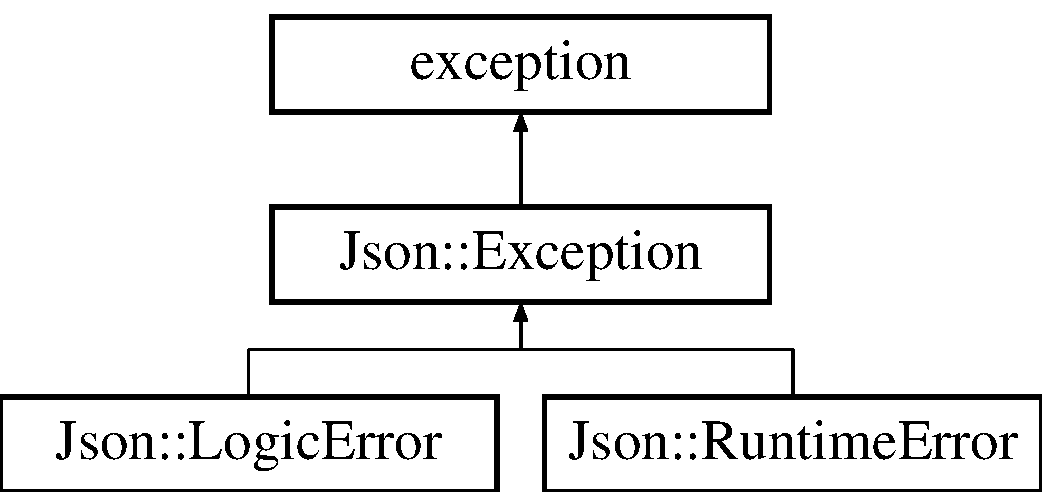
\includegraphics[height=3.000000cm]{class_json_1_1_exception}
\end{center}
\end{figure}
\subsection*{Public Member Functions}
\begin{DoxyCompactItemize}
\item 
\hypertarget{class_json_1_1_exception_a4dd1b9f007bed842e3ef9883d965fe22}{}{\bfseries Exception} (std\+::string const \&msg)\label{class_json_1_1_exception_a4dd1b9f007bed842e3ef9883d965fe22}

\item 
\hypertarget{class_json_1_1_exception_a93032b715e86fc37ad318c60eac4cad7}{}virtual char const $\ast$ {\bfseries what} () const   throw ()\label{class_json_1_1_exception_a93032b715e86fc37ad318c60eac4cad7}

\end{DoxyCompactItemize}
\subsection*{Protected Attributes}
\begin{DoxyCompactItemize}
\item 
\hypertarget{class_json_1_1_exception_a6457bfa979e1bba636ba34605203f6a0}{}std\+::string const {\bfseries msg\+\_\+}\label{class_json_1_1_exception_a6457bfa979e1bba636ba34605203f6a0}

\end{DoxyCompactItemize}


\subsection{Detailed Description}
Base class for all exceptions we throw.

We use nothing but these internally. Of course, S\+T\+L can throw others. 

The documentation for this class was generated from the following files\+:\begin{DoxyCompactItemize}
\item 
/home/robin\+\_\+f/\+Programming/\+Git/\+C\+P\+P/\+Love\+Brains/api/lib/\+A\+N\+N\+Library/include/json/json.\+h\item 
/home/robin\+\_\+f/\+Programming/\+Git/\+C\+P\+P/\+Love\+Brains/api/lib/\+A\+N\+N\+Library/src/json/jsoncpp.\+cc\end{DoxyCompactItemize}

\hypertarget{class_json_1_1_char_reader_1_1_factory}{}\section{Json\+:\+:Char\+Reader\+:\+:Factory Class Reference}
\label{class_json_1_1_char_reader_1_1_factory}\index{Json\+::\+Char\+Reader\+::\+Factory@{Json\+::\+Char\+Reader\+::\+Factory}}
Inheritance diagram for Json\+:\+:Char\+Reader\+:\+:Factory\+:\begin{figure}[H]
\begin{center}
\leavevmode
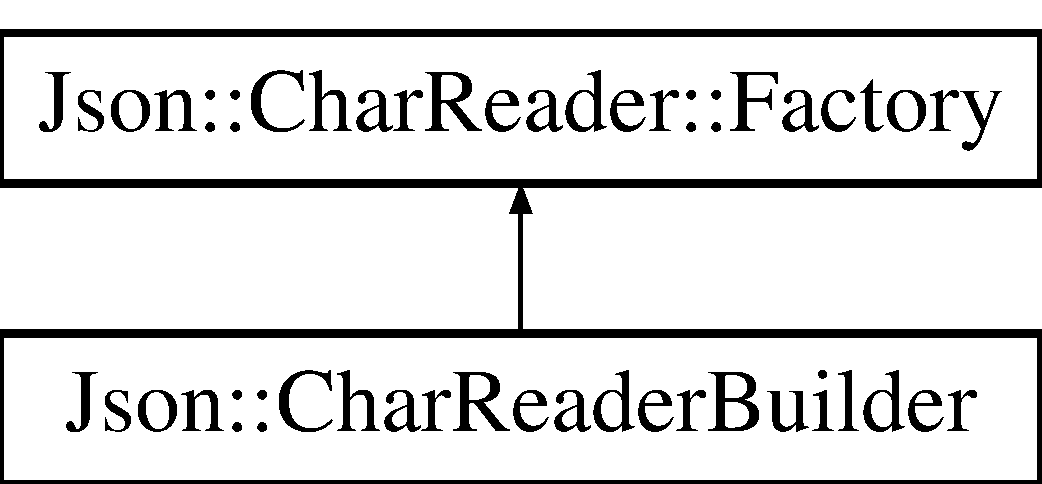
\includegraphics[height=2.000000cm]{class_json_1_1_char_reader_1_1_factory}
\end{center}
\end{figure}
\subsection*{Public Member Functions}
\begin{DoxyCompactItemize}
\item 
virtual \hyperlink{class_json_1_1_char_reader}{Char\+Reader} $\ast$ \hyperlink{class_json_1_1_char_reader_1_1_factory_a497112c51f36a676aeb496c3a91d38d0}{new\+Char\+Reader} () const  =0
\begin{DoxyCompactList}\small\item\em Allocate a \hyperlink{class_json_1_1_char_reader}{Char\+Reader} via operator new(). \end{DoxyCompactList}\end{DoxyCompactItemize}


\subsection{Member Function Documentation}
\hypertarget{class_json_1_1_char_reader_1_1_factory_a497112c51f36a676aeb496c3a91d38d0}{}\index{Json\+::\+Char\+Reader\+::\+Factory@{Json\+::\+Char\+Reader\+::\+Factory}!new\+Char\+Reader@{new\+Char\+Reader}}
\index{new\+Char\+Reader@{new\+Char\+Reader}!Json\+::\+Char\+Reader\+::\+Factory@{Json\+::\+Char\+Reader\+::\+Factory}}
\subsubsection[{new\+Char\+Reader() const  =0}]{\setlength{\rightskip}{0pt plus 5cm}virtual {\bf Char\+Reader}$\ast$ Json\+::\+Char\+Reader\+::\+Factory\+::new\+Char\+Reader (
\begin{DoxyParamCaption}
{}
\end{DoxyParamCaption}
) const\hspace{0.3cm}{\ttfamily [pure virtual]}}\label{class_json_1_1_char_reader_1_1_factory_a497112c51f36a676aeb496c3a91d38d0}


Allocate a \hyperlink{class_json_1_1_char_reader}{Char\+Reader} via operator new(). 


\begin{DoxyExceptions}{Exceptions}
{\em std\+::exception} & if something goes wrong (e.\+g. invalid settings) \\
\hline
\end{DoxyExceptions}


Implemented in \hyperlink{class_json_1_1_char_reader_builder_a3e3c9f4aeb07023ef0c5f6255003078a}{Json\+::\+Char\+Reader\+Builder}.



The documentation for this class was generated from the following file\+:\begin{DoxyCompactItemize}
\item 
/home/robin\+\_\+f/\+Programming/\+Git/\+C\+P\+P/\+Love\+Brains/api/lib/\+A\+N\+N\+Library/include/json/json.\+h\end{DoxyCompactItemize}

\section{Json\+:\+:Stream\+Writer\+:\+:Factory Class Reference}
\label{class_json_1_1_stream_writer_1_1_factory}\index{Json\+::\+Stream\+Writer\+::\+Factory@{Json\+::\+Stream\+Writer\+::\+Factory}}


A simple abstract factory.  




{\ttfamily \#include $<$json.\+h$>$}

Inheritance diagram for Json\+:\+:Stream\+Writer\+:\+:Factory\+:\begin{figure}[H]
\begin{center}
\leavevmode
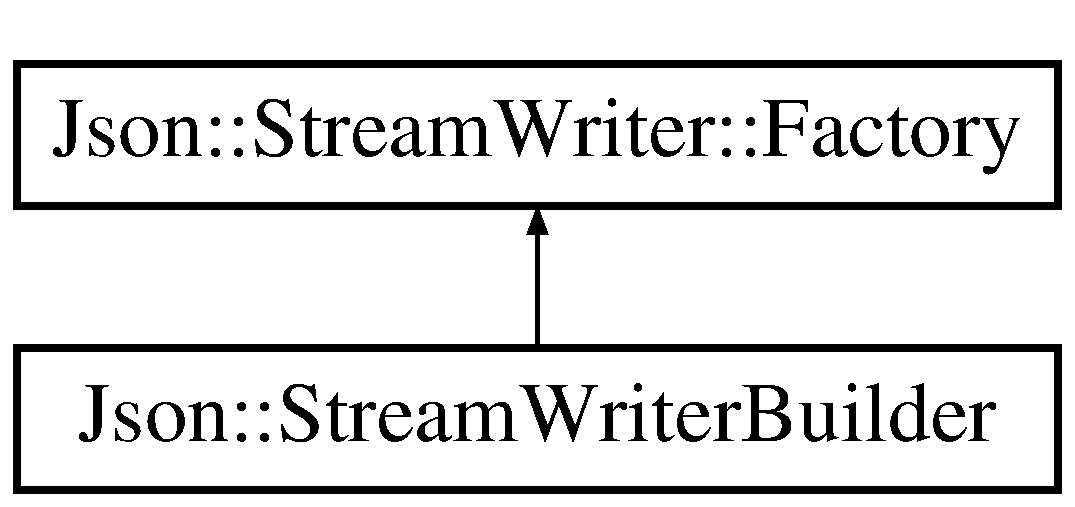
\includegraphics[height=1.590909cm]{class_json_1_1_stream_writer_1_1_factory}
\end{center}
\end{figure}
\subsection*{Public Member Functions}
\begin{DoxyCompactItemize}
\item 
virtual {\bf Stream\+Writer} $\ast$ {\bf new\+Stream\+Writer} () const  =0
\begin{DoxyCompactList}\small\item\em Allocate a \doxyref{Char\+Reader}{p.}{class_json_1_1_char_reader} via operator new(). \end{DoxyCompactList}\item 
virtual {\bf Stream\+Writer} $\ast$ {\bf new\+Stream\+Writer} () const  =0
\begin{DoxyCompactList}\small\item\em Allocate a \doxyref{Char\+Reader}{p.}{class_json_1_1_char_reader} via operator new(). \end{DoxyCompactList}\item 
virtual {\bf Stream\+Writer} $\ast$ {\bf new\+Stream\+Writer} () const  =0
\begin{DoxyCompactList}\small\item\em Allocate a \doxyref{Char\+Reader}{p.}{class_json_1_1_char_reader} via operator new(). \end{DoxyCompactList}\item 
virtual {\bf Stream\+Writer} $\ast$ {\bf new\+Stream\+Writer} () const  =0
\begin{DoxyCompactList}\small\item\em Allocate a \doxyref{Char\+Reader}{p.}{class_json_1_1_char_reader} via operator new(). \end{DoxyCompactList}\end{DoxyCompactItemize}


\subsection{Detailed Description}
A simple abstract factory. 

\subsection{Member Function Documentation}
\index{Json\+::\+Stream\+Writer\+::\+Factory@{Json\+::\+Stream\+Writer\+::\+Factory}!new\+Stream\+Writer@{new\+Stream\+Writer}}
\index{new\+Stream\+Writer@{new\+Stream\+Writer}!Json\+::\+Stream\+Writer\+::\+Factory@{Json\+::\+Stream\+Writer\+::\+Factory}}
\subsubsection[{new\+Stream\+Writer() const  =0}]{\setlength{\rightskip}{0pt plus 5cm}virtual {\bf Stream\+Writer}$\ast$ Json\+::\+Stream\+Writer\+::\+Factory\+::new\+Stream\+Writer (
\begin{DoxyParamCaption}
{}
\end{DoxyParamCaption}
) const\hspace{0.3cm}{\ttfamily [pure virtual]}}\label{class_json_1_1_stream_writer_1_1_factory_a0fca8d713eb8949ca3ebb35e67f23b1a}


Allocate a \doxyref{Char\+Reader}{p.}{class_json_1_1_char_reader} via operator new(). 


\begin{DoxyExceptions}{Exceptions}
{\em std\+::exception} & if something goes wrong (e.\+g. invalid settings) \\
\hline
\end{DoxyExceptions}


Implemented in {\bf Json\+::\+Stream\+Writer\+Builder} \doxyref{}{p.}{class_json_1_1_stream_writer_builder_a96c85792f6680835094917ee93915e4b}, {\bf Json\+::\+Stream\+Writer\+Builder} \doxyref{}{p.}{class_json_1_1_stream_writer_builder_ac7dfbb1cde1c3b9fa0781c1b8885bdff}, {\bf Json\+::\+Stream\+Writer\+Builder} \doxyref{}{p.}{class_json_1_1_stream_writer_builder_ac7dfbb1cde1c3b9fa0781c1b8885bdff}, and {\bf Json\+::\+Stream\+Writer\+Builder} \doxyref{}{p.}{class_json_1_1_stream_writer_builder_ac7dfbb1cde1c3b9fa0781c1b8885bdff}.

\index{Json\+::\+Stream\+Writer\+::\+Factory@{Json\+::\+Stream\+Writer\+::\+Factory}!new\+Stream\+Writer@{new\+Stream\+Writer}}
\index{new\+Stream\+Writer@{new\+Stream\+Writer}!Json\+::\+Stream\+Writer\+::\+Factory@{Json\+::\+Stream\+Writer\+::\+Factory}}
\subsubsection[{new\+Stream\+Writer() const  =0}]{\setlength{\rightskip}{0pt plus 5cm}virtual {\bf Stream\+Writer}$\ast$ Json\+::\+Stream\+Writer\+::\+Factory\+::new\+Stream\+Writer (
\begin{DoxyParamCaption}
{}
\end{DoxyParamCaption}
) const\hspace{0.3cm}{\ttfamily [pure virtual]}}\label{class_json_1_1_stream_writer_1_1_factory_a0fca8d713eb8949ca3ebb35e67f23b1a}


Allocate a \doxyref{Char\+Reader}{p.}{class_json_1_1_char_reader} via operator new(). 


\begin{DoxyExceptions}{Exceptions}
{\em std\+::exception} & if something goes wrong (e.\+g. invalid settings) \\
\hline
\end{DoxyExceptions}


Implemented in {\bf Json\+::\+Stream\+Writer\+Builder} \doxyref{}{p.}{class_json_1_1_stream_writer_builder_a96c85792f6680835094917ee93915e4b}, {\bf Json\+::\+Stream\+Writer\+Builder} \doxyref{}{p.}{class_json_1_1_stream_writer_builder_ac7dfbb1cde1c3b9fa0781c1b8885bdff}, {\bf Json\+::\+Stream\+Writer\+Builder} \doxyref{}{p.}{class_json_1_1_stream_writer_builder_ac7dfbb1cde1c3b9fa0781c1b8885bdff}, and {\bf Json\+::\+Stream\+Writer\+Builder} \doxyref{}{p.}{class_json_1_1_stream_writer_builder_ac7dfbb1cde1c3b9fa0781c1b8885bdff}.

\index{Json\+::\+Stream\+Writer\+::\+Factory@{Json\+::\+Stream\+Writer\+::\+Factory}!new\+Stream\+Writer@{new\+Stream\+Writer}}
\index{new\+Stream\+Writer@{new\+Stream\+Writer}!Json\+::\+Stream\+Writer\+::\+Factory@{Json\+::\+Stream\+Writer\+::\+Factory}}
\subsubsection[{new\+Stream\+Writer() const  =0}]{\setlength{\rightskip}{0pt plus 5cm}virtual {\bf Stream\+Writer}$\ast$ Json\+::\+Stream\+Writer\+::\+Factory\+::new\+Stream\+Writer (
\begin{DoxyParamCaption}
{}
\end{DoxyParamCaption}
) const\hspace{0.3cm}{\ttfamily [pure virtual]}}\label{class_json_1_1_stream_writer_1_1_factory_a0fca8d713eb8949ca3ebb35e67f23b1a}


Allocate a \doxyref{Char\+Reader}{p.}{class_json_1_1_char_reader} via operator new(). 


\begin{DoxyExceptions}{Exceptions}
{\em std\+::exception} & if something goes wrong (e.\+g. invalid settings) \\
\hline
\end{DoxyExceptions}


Implemented in {\bf Json\+::\+Stream\+Writer\+Builder} \doxyref{}{p.}{class_json_1_1_stream_writer_builder_a96c85792f6680835094917ee93915e4b}, {\bf Json\+::\+Stream\+Writer\+Builder} \doxyref{}{p.}{class_json_1_1_stream_writer_builder_ac7dfbb1cde1c3b9fa0781c1b8885bdff}, {\bf Json\+::\+Stream\+Writer\+Builder} \doxyref{}{p.}{class_json_1_1_stream_writer_builder_ac7dfbb1cde1c3b9fa0781c1b8885bdff}, and {\bf Json\+::\+Stream\+Writer\+Builder} \doxyref{}{p.}{class_json_1_1_stream_writer_builder_ac7dfbb1cde1c3b9fa0781c1b8885bdff}.

\index{Json\+::\+Stream\+Writer\+::\+Factory@{Json\+::\+Stream\+Writer\+::\+Factory}!new\+Stream\+Writer@{new\+Stream\+Writer}}
\index{new\+Stream\+Writer@{new\+Stream\+Writer}!Json\+::\+Stream\+Writer\+::\+Factory@{Json\+::\+Stream\+Writer\+::\+Factory}}
\subsubsection[{new\+Stream\+Writer() const  =0}]{\setlength{\rightskip}{0pt plus 5cm}virtual {\bf Stream\+Writer}$\ast$ Json\+::\+Stream\+Writer\+::\+Factory\+::new\+Stream\+Writer (
\begin{DoxyParamCaption}
{}
\end{DoxyParamCaption}
) const\hspace{0.3cm}{\ttfamily [pure virtual]}}\label{class_json_1_1_stream_writer_1_1_factory_a0fca8d713eb8949ca3ebb35e67f23b1a}


Allocate a \doxyref{Char\+Reader}{p.}{class_json_1_1_char_reader} via operator new(). 


\begin{DoxyExceptions}{Exceptions}
{\em std\+::exception} & if something goes wrong (e.\+g. invalid settings) \\
\hline
\end{DoxyExceptions}


Implemented in {\bf Json\+::\+Stream\+Writer\+Builder} \doxyref{}{p.}{class_json_1_1_stream_writer_builder_a96c85792f6680835094917ee93915e4b}, {\bf Json\+::\+Stream\+Writer\+Builder} \doxyref{}{p.}{class_json_1_1_stream_writer_builder_ac7dfbb1cde1c3b9fa0781c1b8885bdff}, {\bf Json\+::\+Stream\+Writer\+Builder} \doxyref{}{p.}{class_json_1_1_stream_writer_builder_ac7dfbb1cde1c3b9fa0781c1b8885bdff}, and {\bf Json\+::\+Stream\+Writer\+Builder} \doxyref{}{p.}{class_json_1_1_stream_writer_builder_ac7dfbb1cde1c3b9fa0781c1b8885bdff}.



The documentation for this class was generated from the following files\+:\begin{DoxyCompactItemize}
\item 
api/lib/\+A\+N\+N\+Library/include/json/json.\+h\item 
api/lib/\+A\+N\+N\+Library/src/json/jsoncpp.\+cc\end{DoxyCompactItemize}

\section{Json\+:\+:Fast\+Writer Class Reference}
\label{class_json_1_1_fast_writer}\index{Json\+::\+Fast\+Writer@{Json\+::\+Fast\+Writer}}


Outputs a \doxyref{Value}{p.}{class_json_1_1_value} in {\tt J\+S\+O\+N} format without formatting (not human friendly).  




{\ttfamily \#include $<$json.\+h$>$}

Inheritance diagram for Json\+:\+:Fast\+Writer\+:\begin{figure}[H]
\begin{center}
\leavevmode
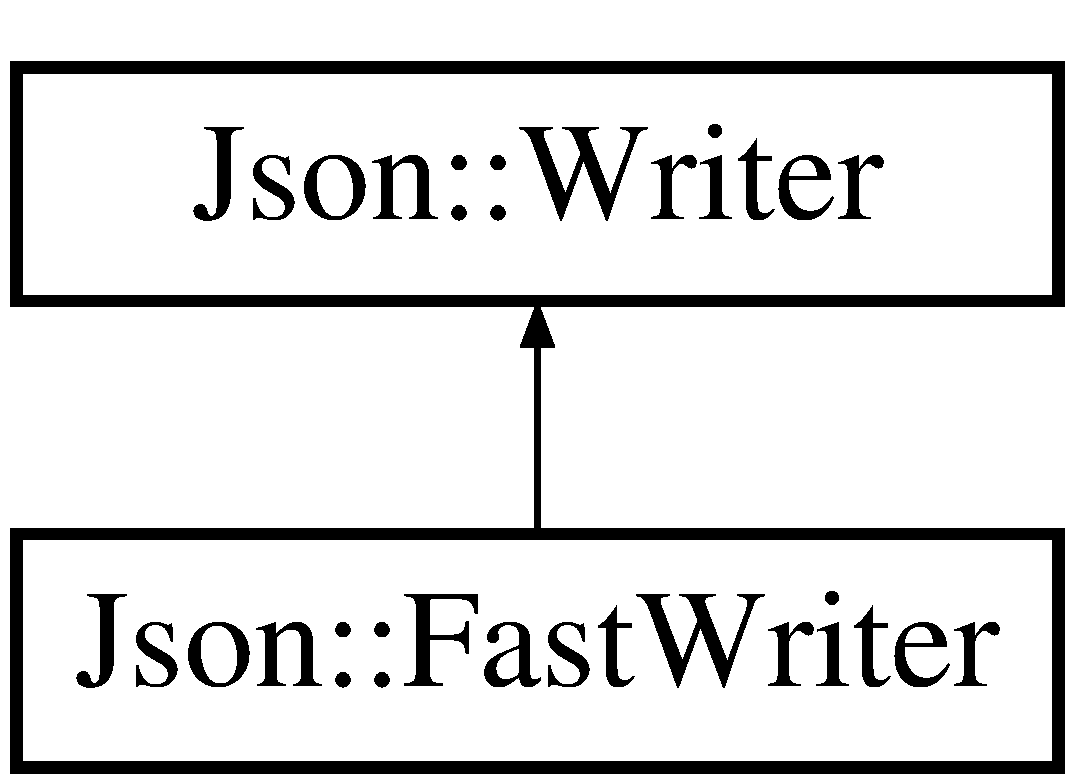
\includegraphics[height=2.000000cm]{class_json_1_1_fast_writer}
\end{center}
\end{figure}
\subsection*{Public Member Functions}
\begin{DoxyCompactItemize}
\item 
void {\bfseries enable\+Y\+A\+M\+L\+Compatibility} ()\label{class_json_1_1_fast_writer_a78d98e9f76d33660ad6e6a1abe287d45}

\item 
void {\bf drop\+Null\+Placeholders} ()\label{class_json_1_1_fast_writer_a6e93d8dce951e408517311026a065b40}

\begin{DoxyCompactList}\small\item\em Drop the \char`\"{}null\char`\"{} string from the writer\textquotesingle{}s output for null\+Values. Strictly speaking, this is not valid J\+S\+O\+N. But when the output is being fed to a browser\textquotesingle{}s Javascript, it makes for smaller output and the browser can handle the output just fine. \end{DoxyCompactList}\item 
void {\bfseries omit\+Ending\+Line\+Feed} ()\label{class_json_1_1_fast_writer_af4ee077d365d75941fb2688d97207a55}

\item 
virtual std\+::string {\bfseries write} (const {\bf Value} \&root)\label{class_json_1_1_fast_writer_aa66218a56447222f91d64db618935a19}

\item 
void {\bfseries enable\+Y\+A\+M\+L\+Compatibility} ()\label{class_json_1_1_fast_writer_a78d98e9f76d33660ad6e6a1abe287d45}

\item 
void {\bf drop\+Null\+Placeholders} ()\label{class_json_1_1_fast_writer_a6e93d8dce951e408517311026a065b40}

\begin{DoxyCompactList}\small\item\em Drop the \char`\"{}null\char`\"{} string from the writer\textquotesingle{}s output for null\+Values. Strictly speaking, this is not valid J\+S\+O\+N. But when the output is being fed to a browser\textquotesingle{}s Javascript, it makes for smaller output and the browser can handle the output just fine. \end{DoxyCompactList}\item 
void {\bfseries omit\+Ending\+Line\+Feed} ()\label{class_json_1_1_fast_writer_af4ee077d365d75941fb2688d97207a55}

\item 
virtual std\+::string {\bfseries write} (const {\bf Value} \&root)\label{class_json_1_1_fast_writer_a0f64b9e1fce6b743aad3f100cfc33427}

\item 
void {\bfseries enable\+Y\+A\+M\+L\+Compatibility} ()\label{class_json_1_1_fast_writer_a78d98e9f76d33660ad6e6a1abe287d45}

\item 
void {\bf drop\+Null\+Placeholders} ()\label{class_json_1_1_fast_writer_a6e93d8dce951e408517311026a065b40}

\begin{DoxyCompactList}\small\item\em Drop the \char`\"{}null\char`\"{} string from the writer\textquotesingle{}s output for null\+Values. Strictly speaking, this is not valid J\+S\+O\+N. But when the output is being fed to a browser\textquotesingle{}s Javascript, it makes for smaller output and the browser can handle the output just fine. \end{DoxyCompactList}\item 
void {\bfseries omit\+Ending\+Line\+Feed} ()\label{class_json_1_1_fast_writer_af4ee077d365d75941fb2688d97207a55}

\item 
virtual std\+::string {\bfseries write} (const {\bf Value} \&root)\label{class_json_1_1_fast_writer_a0f64b9e1fce6b743aad3f100cfc33427}

\item 
void {\bfseries enable\+Y\+A\+M\+L\+Compatibility} ()\label{class_json_1_1_fast_writer_a78d98e9f76d33660ad6e6a1abe287d45}

\item 
void {\bf drop\+Null\+Placeholders} ()\label{class_json_1_1_fast_writer_a6e93d8dce951e408517311026a065b40}

\begin{DoxyCompactList}\small\item\em Drop the \char`\"{}null\char`\"{} string from the writer\textquotesingle{}s output for null\+Values. Strictly speaking, this is not valid J\+S\+O\+N. But when the output is being fed to a browser\textquotesingle{}s Javascript, it makes for smaller output and the browser can handle the output just fine. \end{DoxyCompactList}\item 
void {\bfseries omit\+Ending\+Line\+Feed} ()\label{class_json_1_1_fast_writer_af4ee077d365d75941fb2688d97207a55}

\item 
virtual std\+::string {\bfseries write} (const {\bf Value} \&root)\label{class_json_1_1_fast_writer_a0f64b9e1fce6b743aad3f100cfc33427}

\end{DoxyCompactItemize}


\subsection{Detailed Description}
Outputs a \doxyref{Value}{p.}{class_json_1_1_value} in {\tt J\+S\+O\+N} format without formatting (not human friendly). 

The J\+S\+O\+N document is written in a single line. It is not intended for \textquotesingle{}human\textquotesingle{} consumption, but may be usefull to support feature such as R\+P\+C where bandwith is limited. \begin{DoxySeeAlso}{See also}
\doxyref{Reader}{p.}{class_json_1_1_reader}, \doxyref{Value}{p.}{class_json_1_1_value} 
\end{DoxySeeAlso}
\begin{DoxyRefDesc}{Deprecated}
\item[{\bf Deprecated}]Use \doxyref{Stream\+Writer\+Builder}{p.}{class_json_1_1_stream_writer_builder}. \end{DoxyRefDesc}


The J\+S\+O\+N document is written in a single line. It is not intended for \textquotesingle{}human\textquotesingle{} consumption, but may be usefull to support feature such as R\+P\+C where bandwith is limited. \begin{DoxySeeAlso}{See also}
\doxyref{Reader}{p.}{class_json_1_1_reader}, \doxyref{Value}{p.}{class_json_1_1_value} 
\end{DoxySeeAlso}
\begin{DoxyRefDesc}{Deprecated}
\item[{\bf Deprecated}]Use \doxyref{Stream\+Writer\+Builder}{p.}{class_json_1_1_stream_writer_builder}. \end{DoxyRefDesc}


The J\+S\+O\+N document is written in a single line. It is not intended for \textquotesingle{}human\textquotesingle{} consumption, but may be usefull to support feature such as R\+P\+C where bandwith is limited. \begin{DoxySeeAlso}{See also}
\doxyref{Reader}{p.}{class_json_1_1_reader}, \doxyref{Value}{p.}{class_json_1_1_value} 
\end{DoxySeeAlso}
\begin{DoxyRefDesc}{Deprecated}
\item[{\bf Deprecated}]Use \doxyref{Stream\+Writer\+Builder}{p.}{class_json_1_1_stream_writer_builder}. \end{DoxyRefDesc}


The J\+S\+O\+N document is written in a single line. It is not intended for \textquotesingle{}human\textquotesingle{} consumption, but may be usefull to support feature such as R\+P\+C where bandwith is limited. \begin{DoxySeeAlso}{See also}
\doxyref{Reader}{p.}{class_json_1_1_reader}, \doxyref{Value}{p.}{class_json_1_1_value} 
\end{DoxySeeAlso}
\begin{DoxyRefDesc}{Deprecated}
\item[{\bf Deprecated}]Use \doxyref{Stream\+Writer\+Builder}{p.}{class_json_1_1_stream_writer_builder}. \end{DoxyRefDesc}


The documentation for this class was generated from the following files\+:\begin{DoxyCompactItemize}
\item 
/home/robin\+\_\+f/\+Programming/\+Git/\+C\+P\+P/\+Love\+Brains/api/lib/\+A\+N\+N\+Library/include/json/json.\+h\item 
/home/robin\+\_\+f/\+Programming/\+Git/\+C\+P\+P/\+Love\+Brains/api/lib/\+A\+N\+N\+Library/src/json/jsoncpp.\+cc\end{DoxyCompactItemize}

\section{Json\+:\+:Features Class Reference}
\label{class_json_1_1_features}\index{Json\+::\+Features@{Json\+::\+Features}}


Configuration passed to reader and writer. This configuration object can be used to force the \doxyref{Reader}{p.}{class_json_1_1_reader} or \doxyref{Writer}{p.}{class_json_1_1_writer} to behave in a standard conforming way.  




{\ttfamily \#include $<$json.\+h$>$}

\subsection*{Public Member Functions}
\begin{DoxyCompactItemize}
\item 
{\bf Features} ()\label{class_json_1_1_features_ad15a091cb61bb31323299a95970d2644}

\begin{DoxyCompactList}\small\item\em Initialize the configuration like Json\+Config\+::all\+Features;. \end{DoxyCompactList}\item 
{\bf Features} ()\label{class_json_1_1_features_ad15a091cb61bb31323299a95970d2644}

\begin{DoxyCompactList}\small\item\em Initialize the configuration like Json\+Config\+::all\+Features;. \end{DoxyCompactList}\item 
{\bf Features} ()\label{class_json_1_1_features_ad15a091cb61bb31323299a95970d2644}

\begin{DoxyCompactList}\small\item\em Initialize the configuration like Json\+Config\+::all\+Features;. \end{DoxyCompactList}\item 
{\bf Features} ()\label{class_json_1_1_features_ad15a091cb61bb31323299a95970d2644}

\begin{DoxyCompactList}\small\item\em Initialize the configuration like Json\+Config\+::all\+Features;. \end{DoxyCompactList}\end{DoxyCompactItemize}
\subsection*{Static Public Member Functions}
\begin{DoxyCompactItemize}
\item 
static {\bf Features} {\bf all} ()
\begin{DoxyCompactList}\small\item\em A configuration that allows all features and assumes all strings are U\+T\+F-\/8. \end{DoxyCompactList}\item 
static {\bf Features} {\bf strict\+Mode} ()
\begin{DoxyCompactList}\small\item\em A configuration that is strictly compatible with the J\+S\+O\+N specification. \end{DoxyCompactList}\item 
static {\bf Features} {\bf all} ()
\begin{DoxyCompactList}\small\item\em A configuration that allows all features and assumes all strings are U\+T\+F-\/8. \end{DoxyCompactList}\item 
static {\bf Features} {\bf strict\+Mode} ()
\begin{DoxyCompactList}\small\item\em A configuration that is strictly compatible with the J\+S\+O\+N specification. \end{DoxyCompactList}\item 
static {\bf Features} {\bf all} ()
\begin{DoxyCompactList}\small\item\em A configuration that allows all features and assumes all strings are U\+T\+F-\/8. \end{DoxyCompactList}\item 
static {\bf Features} {\bf strict\+Mode} ()
\begin{DoxyCompactList}\small\item\em A configuration that is strictly compatible with the J\+S\+O\+N specification. \end{DoxyCompactList}\item 
static {\bf Features} {\bf all} ()
\begin{DoxyCompactList}\small\item\em A configuration that allows all features and assumes all strings are U\+T\+F-\/8. \end{DoxyCompactList}\item 
static {\bf Features} {\bf strict\+Mode} ()
\begin{DoxyCompactList}\small\item\em A configuration that is strictly compatible with the J\+S\+O\+N specification. \end{DoxyCompactList}\end{DoxyCompactItemize}
\subsection*{Public Attributes}
\begin{DoxyCompactItemize}
\item 
bool {\bf allow\+Comments\+\_\+}\label{class_json_1_1_features_a33afd389719624b6bdb23950b3c346c9}

\begin{DoxyCompactList}\small\item\em {\ttfamily true} if comments are allowed. Default\+: {\ttfamily true}. \end{DoxyCompactList}\item 
bool {\bf strict\+Root\+\_\+}
\item 
bool {\bf allow\+Dropped\+Null\+Placeholders\+\_\+}\label{class_json_1_1_features_a5076aa72c05c7596ac339ede36c97a6a}

\begin{DoxyCompactList}\small\item\em {\ttfamily true} if dropped null placeholders are allowed. Default\+: {\ttfamily false}. \end{DoxyCompactList}\item 
bool {\bf allow\+Numeric\+Keys\+\_\+}\label{class_json_1_1_features_aff3cb16b79d15d3d761b11a0dd6d4d6b}

\begin{DoxyCompactList}\small\item\em {\ttfamily true} if numeric object key are allowed. Default\+: {\ttfamily false}. \end{DoxyCompactList}\end{DoxyCompactItemize}


\subsection{Detailed Description}
Configuration passed to reader and writer. This configuration object can be used to force the \doxyref{Reader}{p.}{class_json_1_1_reader} or \doxyref{Writer}{p.}{class_json_1_1_writer} to behave in a standard conforming way. 

\subsection{Member Function Documentation}
\index{Json\+::\+Features@{Json\+::\+Features}!all@{all}}
\index{all@{all}!Json\+::\+Features@{Json\+::\+Features}}
\subsubsection[{all()}]{\setlength{\rightskip}{0pt plus 5cm}{\bf Features} Json\+::\+Features\+::all (
\begin{DoxyParamCaption}
{}
\end{DoxyParamCaption}
)\hspace{0.3cm}{\ttfamily [static]}}\label{class_json_1_1_features_a63894da6e2c100b38741fa933f3d33ae}


A configuration that allows all features and assumes all strings are U\+T\+F-\/8. 


\begin{DoxyItemize}
\item C \& C++ comments are allowed
\item Root object can be any J\+S\+O\+N value
\item Assumes \doxyref{Value}{p.}{class_json_1_1_value} strings are encoded in U\+T\+F-\/8 
\end{DoxyItemize}\index{Json\+::\+Features@{Json\+::\+Features}!all@{all}}
\index{all@{all}!Json\+::\+Features@{Json\+::\+Features}}
\subsubsection[{all()}]{\setlength{\rightskip}{0pt plus 5cm}static {\bf Features} Json\+::\+Features\+::all (
\begin{DoxyParamCaption}
{}
\end{DoxyParamCaption}
)\hspace{0.3cm}{\ttfamily [static]}}\label{class_json_1_1_features_a9f17db1b4ebbef8c645825344959481b}


A configuration that allows all features and assumes all strings are U\+T\+F-\/8. 


\begin{DoxyItemize}
\item C \& C++ comments are allowed
\item Root object can be any J\+S\+O\+N value
\item Assumes \doxyref{Value}{p.}{class_json_1_1_value} strings are encoded in U\+T\+F-\/8 
\end{DoxyItemize}\index{Json\+::\+Features@{Json\+::\+Features}!all@{all}}
\index{all@{all}!Json\+::\+Features@{Json\+::\+Features}}
\subsubsection[{all()}]{\setlength{\rightskip}{0pt plus 5cm}static {\bf Features} Json\+::\+Features\+::all (
\begin{DoxyParamCaption}
{}
\end{DoxyParamCaption}
)\hspace{0.3cm}{\ttfamily [static]}}\label{class_json_1_1_features_a9f17db1b4ebbef8c645825344959481b}


A configuration that allows all features and assumes all strings are U\+T\+F-\/8. 


\begin{DoxyItemize}
\item C \& C++ comments are allowed
\item Root object can be any J\+S\+O\+N value
\item Assumes \doxyref{Value}{p.}{class_json_1_1_value} strings are encoded in U\+T\+F-\/8 
\end{DoxyItemize}\index{Json\+::\+Features@{Json\+::\+Features}!all@{all}}
\index{all@{all}!Json\+::\+Features@{Json\+::\+Features}}
\subsubsection[{all()}]{\setlength{\rightskip}{0pt plus 5cm}static {\bf Features} Json\+::\+Features\+::all (
\begin{DoxyParamCaption}
{}
\end{DoxyParamCaption}
)\hspace{0.3cm}{\ttfamily [static]}}\label{class_json_1_1_features_a9f17db1b4ebbef8c645825344959481b}


A configuration that allows all features and assumes all strings are U\+T\+F-\/8. 


\begin{DoxyItemize}
\item C \& C++ comments are allowed
\item Root object can be any J\+S\+O\+N value
\item Assumes \doxyref{Value}{p.}{class_json_1_1_value} strings are encoded in U\+T\+F-\/8 
\end{DoxyItemize}\index{Json\+::\+Features@{Json\+::\+Features}!strict\+Mode@{strict\+Mode}}
\index{strict\+Mode@{strict\+Mode}!Json\+::\+Features@{Json\+::\+Features}}
\subsubsection[{strict\+Mode()}]{\setlength{\rightskip}{0pt plus 5cm}{\bf Features} Json\+::\+Features\+::strict\+Mode (
\begin{DoxyParamCaption}
{}
\end{DoxyParamCaption}
)\hspace{0.3cm}{\ttfamily [static]}}\label{class_json_1_1_features_ae23176c14b2e79e81fb61fb1a8ab58ee}


A configuration that is strictly compatible with the J\+S\+O\+N specification. 


\begin{DoxyItemize}
\item Comments are forbidden.
\item Root object must be either an array or an object value.
\item Assumes \doxyref{Value}{p.}{class_json_1_1_value} strings are encoded in U\+T\+F-\/8 
\end{DoxyItemize}\index{Json\+::\+Features@{Json\+::\+Features}!strict\+Mode@{strict\+Mode}}
\index{strict\+Mode@{strict\+Mode}!Json\+::\+Features@{Json\+::\+Features}}
\subsubsection[{strict\+Mode()}]{\setlength{\rightskip}{0pt plus 5cm}static {\bf Features} Json\+::\+Features\+::strict\+Mode (
\begin{DoxyParamCaption}
{}
\end{DoxyParamCaption}
)\hspace{0.3cm}{\ttfamily [static]}}\label{class_json_1_1_features_aed3a2845df0cfd2ebe7338442361bd13}


A configuration that is strictly compatible with the J\+S\+O\+N specification. 


\begin{DoxyItemize}
\item Comments are forbidden.
\item Root object must be either an array or an object value.
\item Assumes \doxyref{Value}{p.}{class_json_1_1_value} strings are encoded in U\+T\+F-\/8 
\end{DoxyItemize}\index{Json\+::\+Features@{Json\+::\+Features}!strict\+Mode@{strict\+Mode}}
\index{strict\+Mode@{strict\+Mode}!Json\+::\+Features@{Json\+::\+Features}}
\subsubsection[{strict\+Mode()}]{\setlength{\rightskip}{0pt plus 5cm}static {\bf Features} Json\+::\+Features\+::strict\+Mode (
\begin{DoxyParamCaption}
{}
\end{DoxyParamCaption}
)\hspace{0.3cm}{\ttfamily [static]}}\label{class_json_1_1_features_aed3a2845df0cfd2ebe7338442361bd13}


A configuration that is strictly compatible with the J\+S\+O\+N specification. 


\begin{DoxyItemize}
\item Comments are forbidden.
\item Root object must be either an array or an object value.
\item Assumes \doxyref{Value}{p.}{class_json_1_1_value} strings are encoded in U\+T\+F-\/8 
\end{DoxyItemize}\index{Json\+::\+Features@{Json\+::\+Features}!strict\+Mode@{strict\+Mode}}
\index{strict\+Mode@{strict\+Mode}!Json\+::\+Features@{Json\+::\+Features}}
\subsubsection[{strict\+Mode()}]{\setlength{\rightskip}{0pt plus 5cm}static {\bf Features} Json\+::\+Features\+::strict\+Mode (
\begin{DoxyParamCaption}
{}
\end{DoxyParamCaption}
)\hspace{0.3cm}{\ttfamily [static]}}\label{class_json_1_1_features_aed3a2845df0cfd2ebe7338442361bd13}


A configuration that is strictly compatible with the J\+S\+O\+N specification. 


\begin{DoxyItemize}
\item Comments are forbidden.
\item Root object must be either an array or an object value.
\item Assumes \doxyref{Value}{p.}{class_json_1_1_value} strings are encoded in U\+T\+F-\/8 
\end{DoxyItemize}

\subsection{Member Data Documentation}
\index{Json\+::\+Features@{Json\+::\+Features}!strict\+Root\+\_\+@{strict\+Root\+\_\+}}
\index{strict\+Root\+\_\+@{strict\+Root\+\_\+}!Json\+::\+Features@{Json\+::\+Features}}
\subsubsection[{strict\+Root\+\_\+}]{\setlength{\rightskip}{0pt plus 5cm}bool Json\+::\+Features\+::strict\+Root\+\_\+}\label{class_json_1_1_features_a1162c37a1458adc32582b585b552f9c3}
{\ttfamily true} if root must be either an array or an object value. Default\+: {\ttfamily false}. 

The documentation for this class was generated from the following files\+:\begin{DoxyCompactItemize}
\item 
/home/robin\+\_\+f/\+Programming/\+Git/\+C\+P\+P/\+Love\+Brains/api/lib/\+A\+N\+N\+Library/include/json/json.\+h\item 
/home/robin\+\_\+f/\+Programming/\+Git/\+C\+P\+P/\+Love\+Brains/api/lib/\+A\+N\+N\+Library/src/json/jsoncpp.\+cc\end{DoxyCompactItemize}

\section{Graphics\+:\+:I\+Behavior Class Reference}
\label{class_graphics_1_1_i_behavior}\index{Graphics\+::\+I\+Behavior@{Graphics\+::\+I\+Behavior}}


Define a behavior for a collider.  




{\ttfamily \#include $<$i\+\_\+behavior.\+h$>$}

Inheritance diagram for Graphics\+:\+:I\+Behavior\+:\begin{figure}[H]
\begin{center}
\leavevmode
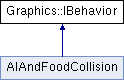
\includegraphics[height=2.000000cm]{class_graphics_1_1_i_behavior}
\end{center}
\end{figure}
\subsection*{Public Member Functions}
\begin{DoxyCompactItemize}
\item 
virtual void {\bfseries Update} ({\bf I\+Object} $\ast$obj)=0\label{class_graphics_1_1_i_behavior_ac341180608014d8ec54c2b775881c191}

\item 
virtual {\bf $\sim$\+I\+Behavior} (void)\label{class_graphics_1_1_i_behavior_a7b7335a435db0c76fc0b596792d3a905}

\begin{DoxyCompactList}\small\item\em Destructor. \end{DoxyCompactList}\item 
virtual void {\bf Update} ({\bf I\+Object} $\ast$obj)=0
\begin{DoxyCompactList}\small\item\em Update the object that have been affected the collider. \end{DoxyCompactList}\item 
virtual void {\bfseries Update} ({\bf I\+Object} $\ast$obj)=0\label{class_graphics_1_1_i_behavior_ac341180608014d8ec54c2b775881c191}

\end{DoxyCompactItemize}


\subsection{Detailed Description}
Define a behavior for a collider. 

\subsection{Member Function Documentation}
\index{Graphics\+::\+I\+Behavior@{Graphics\+::\+I\+Behavior}!Update@{Update}}
\index{Update@{Update}!Graphics\+::\+I\+Behavior@{Graphics\+::\+I\+Behavior}}
\subsubsection[{Update(\+I\+Object $\ast$obj)=0}]{\setlength{\rightskip}{0pt plus 5cm}virtual void Graphics\+::\+I\+Behavior\+::\+Update (
\begin{DoxyParamCaption}
\item[{{\bf I\+Object} $\ast$}]{obj}
\end{DoxyParamCaption}
)\hspace{0.3cm}{\ttfamily [pure virtual]}}\label{class_graphics_1_1_i_behavior_ac341180608014d8ec54c2b775881c191}


Update the object that have been affected the collider. 


\begin{DoxyParams}{Parameters}
{\em obj} & \+: Contains the object that is affected by the collider. \\
\hline
\end{DoxyParams}


The documentation for this class was generated from the following file\+:\begin{DoxyCompactItemize}
\item 
/home/robin\+\_\+f/\+Programming/\+Git/\+C\+P\+P/\+Love\+Brains/api/include/\+Graphics/i\+\_\+behavior.\+h\end{DoxyCompactItemize}

\section{Graphics\+:\+:I\+Brain Class Reference}
\label{class_graphics_1_1_i_brain}\index{Graphics\+::\+I\+Brain@{Graphics\+::\+I\+Brain}}


Define the interface of an object that contains a neural network.  




{\ttfamily \#include $<$i\+\_\+brain.\+h$>$}

Inheritance diagram for Graphics\+:\+:I\+Brain\+:\begin{figure}[H]
\begin{center}
\leavevmode
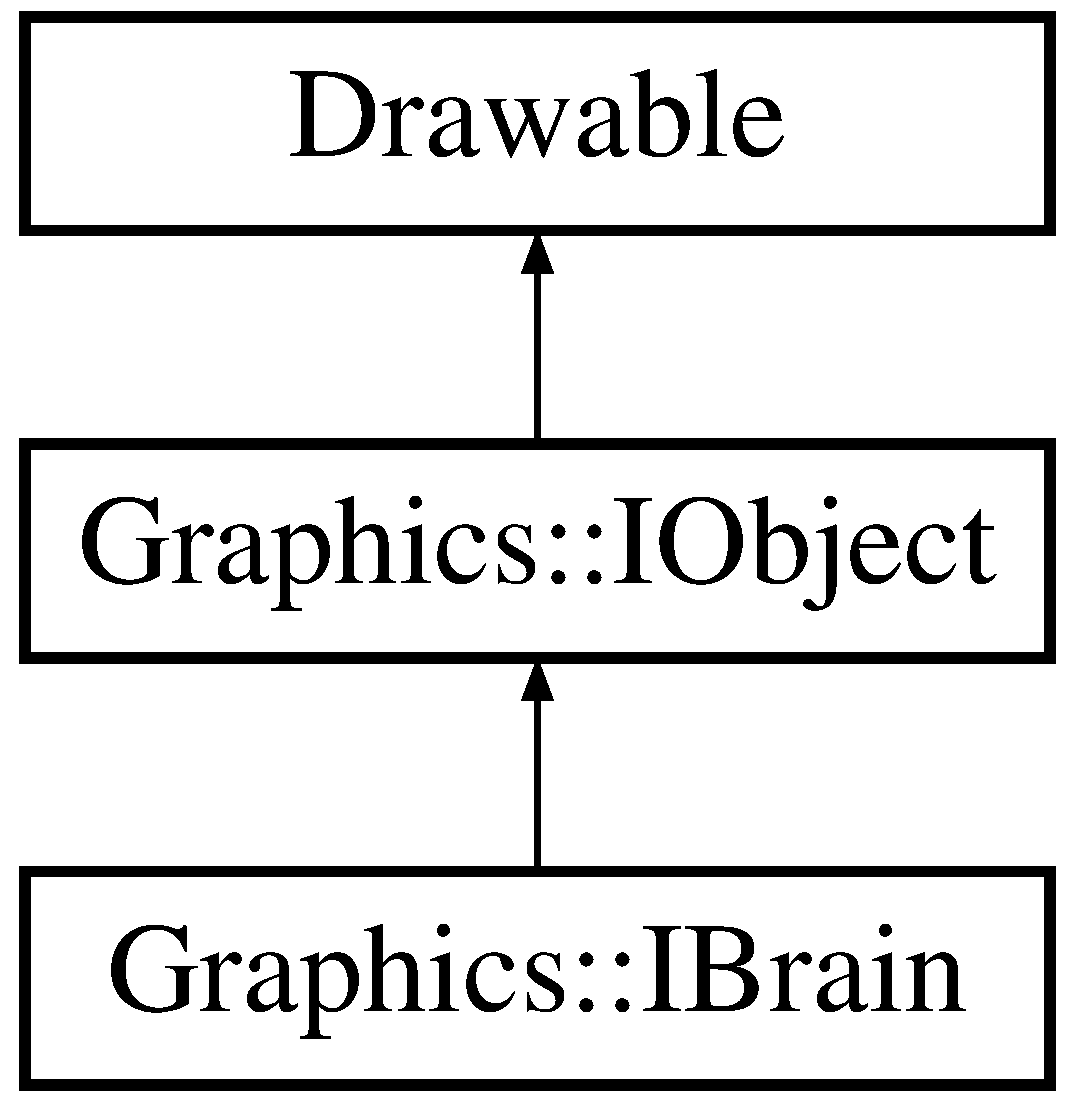
\includegraphics[height=4.188035cm]{class_graphics_1_1_i_brain}
\end{center}
\end{figure}
\subsection*{Public Member Functions}
\begin{DoxyCompactItemize}
\item 
virtual double {\bfseries get\+Fitness} (void) const  =0\label{class_graphics_1_1_i_brain_a45403eb25f611290de9c53eaf7f6e800}

\item 
virtual void {\bfseries set\+Fitness} (double fitness)=0\label{class_graphics_1_1_i_brain_a1fdec2222c5a04a93c6918ed1f271947}

\item 
virtual void {\bfseries set\+Brain} ({\bf G\+A\+N\+N\+::\+A\+N\+N} const \&brain)=0\label{class_graphics_1_1_i_brain_a56c5f2f1f998551b571442b0225986e7}

\item 
virtual void {\bfseries set\+Input} (unsigned int index, double value)=0\label{class_graphics_1_1_i_brain_a768f7a2e586cafbbc7c4c2ae846a52be}

\item 
virtual {\bf $\sim$\+I\+Brain} (void)\label{class_graphics_1_1_i_brain_a9069cd56cdd867929c7f87d90c55f0c8}

\begin{DoxyCompactList}\small\item\em Destructor. \end{DoxyCompactList}\item 
virtual double {\bf get\+Fitness} (void) const  =0
\begin{DoxyCompactList}\small\item\em Get the current fitness of the object. \end{DoxyCompactList}\item 
virtual void {\bf set\+Fitness} (double fitness)=0
\begin{DoxyCompactList}\small\item\em Set the current fitness of the object. \end{DoxyCompactList}\item 
virtual void {\bf set\+Brain} ({\bf G\+A\+N\+N\+::\+A\+N\+N} const \&brain)=0
\begin{DoxyCompactList}\small\item\em Set the current neural network of the object. \end{DoxyCompactList}\item 
virtual void {\bf set\+Input} (unsigned int index, double value)=0
\begin{DoxyCompactList}\small\item\em Set an input for the neural network. \end{DoxyCompactList}\item 
virtual double {\bfseries get\+Fitness} (void) const  =0\label{class_graphics_1_1_i_brain_a45403eb25f611290de9c53eaf7f6e800}

\item 
virtual void {\bfseries set\+Fitness} (double fitness)=0\label{class_graphics_1_1_i_brain_a1fdec2222c5a04a93c6918ed1f271947}

\item 
virtual void {\bfseries set\+Brain} ({\bf G\+A\+N\+N\+::\+A\+N\+N} const \&brain)=0\label{class_graphics_1_1_i_brain_a56c5f2f1f998551b571442b0225986e7}

\item 
virtual void {\bfseries set\+Input} (unsigned int index, double value)=0\label{class_graphics_1_1_i_brain_a768f7a2e586cafbbc7c4c2ae846a52be}

\item 
virtual double {\bfseries get\+Fitness} (void) const  =0\label{class_graphics_1_1_i_brain_a45403eb25f611290de9c53eaf7f6e800}

\item 
virtual void {\bfseries set\+Fitness} (double fitness)=0\label{class_graphics_1_1_i_brain_a1fdec2222c5a04a93c6918ed1f271947}

\item 
virtual void {\bfseries set\+Brain} ({\bf G\+A\+N\+N\+::\+A\+N\+N} const \&brain)=0\label{class_graphics_1_1_i_brain_a56c5f2f1f998551b571442b0225986e7}

\item 
virtual void {\bfseries set\+Input} (unsigned int index, double value)=0\label{class_graphics_1_1_i_brain_a768f7a2e586cafbbc7c4c2ae846a52be}

\end{DoxyCompactItemize}
\subsection*{Additional Inherited Members}


\subsection{Detailed Description}
Define the interface of an object that contains a neural network. 

\subsection{Member Function Documentation}
\index{Graphics\+::\+I\+Brain@{Graphics\+::\+I\+Brain}!get\+Fitness@{get\+Fitness}}
\index{get\+Fitness@{get\+Fitness}!Graphics\+::\+I\+Brain@{Graphics\+::\+I\+Brain}}
\subsubsection[{get\+Fitness(void) const  =0}]{\setlength{\rightskip}{0pt plus 5cm}virtual double Graphics\+::\+I\+Brain\+::get\+Fitness (
\begin{DoxyParamCaption}
\item[{void}]{}
\end{DoxyParamCaption}
) const\hspace{0.3cm}{\ttfamily [pure virtual]}}\label{class_graphics_1_1_i_brain_a45403eb25f611290de9c53eaf7f6e800}


Get the current fitness of the object. 

\begin{DoxyReturn}{Returns}
double 
\end{DoxyReturn}
\index{Graphics\+::\+I\+Brain@{Graphics\+::\+I\+Brain}!set\+Brain@{set\+Brain}}
\index{set\+Brain@{set\+Brain}!Graphics\+::\+I\+Brain@{Graphics\+::\+I\+Brain}}
\subsubsection[{set\+Brain(\+G\+A\+N\+N\+::\+A\+N\+N const \&brain)=0}]{\setlength{\rightskip}{0pt plus 5cm}virtual void Graphics\+::\+I\+Brain\+::set\+Brain (
\begin{DoxyParamCaption}
\item[{{\bf G\+A\+N\+N\+::\+A\+N\+N} const \&}]{brain}
\end{DoxyParamCaption}
)\hspace{0.3cm}{\ttfamily [pure virtual]}}\label{class_graphics_1_1_i_brain_a56c5f2f1f998551b571442b0225986e7}


Set the current neural network of the object. 


\begin{DoxyParams}{Parameters}
{\em brain} & \+: Contains the new neural network. \\
\hline
\end{DoxyParams}
\index{Graphics\+::\+I\+Brain@{Graphics\+::\+I\+Brain}!set\+Fitness@{set\+Fitness}}
\index{set\+Fitness@{set\+Fitness}!Graphics\+::\+I\+Brain@{Graphics\+::\+I\+Brain}}
\subsubsection[{set\+Fitness(double fitness)=0}]{\setlength{\rightskip}{0pt plus 5cm}virtual void Graphics\+::\+I\+Brain\+::set\+Fitness (
\begin{DoxyParamCaption}
\item[{double}]{fitness}
\end{DoxyParamCaption}
)\hspace{0.3cm}{\ttfamily [pure virtual]}}\label{class_graphics_1_1_i_brain_a1fdec2222c5a04a93c6918ed1f271947}


Set the current fitness of the object. 


\begin{DoxyParams}{Parameters}
{\em fitness} & \+: Contains the new fitness of the object. \\
\hline
\end{DoxyParams}
\index{Graphics\+::\+I\+Brain@{Graphics\+::\+I\+Brain}!set\+Input@{set\+Input}}
\index{set\+Input@{set\+Input}!Graphics\+::\+I\+Brain@{Graphics\+::\+I\+Brain}}
\subsubsection[{set\+Input(unsigned int index, double value)=0}]{\setlength{\rightskip}{0pt plus 5cm}virtual void Graphics\+::\+I\+Brain\+::set\+Input (
\begin{DoxyParamCaption}
\item[{unsigned int}]{index, }
\item[{double}]{value}
\end{DoxyParamCaption}
)\hspace{0.3cm}{\ttfamily [pure virtual]}}\label{class_graphics_1_1_i_brain_a768f7a2e586cafbbc7c4c2ae846a52be}


Set an input for the neural network. 


\begin{DoxyParams}{Parameters}
{\em index} & \+: Contains the index of the input. \\
\hline
{\em value} & \+: Contains the input value. \\
\hline
\end{DoxyParams}


The documentation for this class was generated from the following file\+:\begin{DoxyCompactItemize}
\item 
api/include/\+Graphics/i\+\_\+brain.\+h\end{DoxyCompactItemize}

\section{Graphics\+:\+:I\+Collider Class Reference}
\label{class_graphics_1_1_i_collider}\index{Graphics\+::\+I\+Collider@{Graphics\+::\+I\+Collider}}


Define the interface for the collider object.  




{\ttfamily \#include $<$i\+\_\+collider.\+h$>$}

\subsection*{Public Member Functions}
\begin{DoxyCompactItemize}
\item 
virtual {\bf $\sim$\+I\+Collider} ()\label{class_graphics_1_1_i_collider_aa026161123f822795fa64c187b216aa9}

\begin{DoxyCompactList}\small\item\em Destructor. \end{DoxyCompactList}\item 
virtual bool {\bf is\+Valid} (std\+::string const \&obj\+\_\+1, std\+::string const \&obj\+\_\+2)=0
\begin{DoxyCompactList}\small\item\em Verify if the couple of objects is supported by the collider. \end{DoxyCompactList}\item 
virtual bool {\bf is\+Collision} ({\bf I\+Object} $\ast$obj\+\_\+1, {\bf I\+Object} $\ast$obj\+\_\+2)=0
\begin{DoxyCompactList}\small\item\em Compute if the couple of objects is colliding. \end{DoxyCompactList}\item 
virtual {\bf I\+Behavior} $\ast$ {\bf get\+Action} (void) const  =0
\begin{DoxyCompactList}\small\item\em Get the action that the collider will execute. \end{DoxyCompactList}\end{DoxyCompactItemize}


\subsection{Detailed Description}
Define the interface for the collider object. 

\subsection{Member Function Documentation}
\index{Graphics\+::\+I\+Collider@{Graphics\+::\+I\+Collider}!get\+Action@{get\+Action}}
\index{get\+Action@{get\+Action}!Graphics\+::\+I\+Collider@{Graphics\+::\+I\+Collider}}
\subsubsection[{get\+Action(void) const  =0}]{\setlength{\rightskip}{0pt plus 5cm}virtual {\bf I\+Behavior}$\ast$ Graphics\+::\+I\+Collider\+::get\+Action (
\begin{DoxyParamCaption}
\item[{void}]{}
\end{DoxyParamCaption}
) const\hspace{0.3cm}{\ttfamily [pure virtual]}}\label{class_graphics_1_1_i_collider_a80c81a8f9f1212f1053a0613f0f4d943}


Get the action that the collider will execute. 

\begin{DoxyReturn}{Returns}
\doxyref{I\+Behavior}{p.}{class_graphics_1_1_i_behavior} $\ast$ 
\end{DoxyReturn}
\index{Graphics\+::\+I\+Collider@{Graphics\+::\+I\+Collider}!is\+Collision@{is\+Collision}}
\index{is\+Collision@{is\+Collision}!Graphics\+::\+I\+Collider@{Graphics\+::\+I\+Collider}}
\subsubsection[{is\+Collision(\+I\+Object $\ast$obj\+\_\+1, I\+Object $\ast$obj\+\_\+2)=0}]{\setlength{\rightskip}{0pt plus 5cm}virtual bool Graphics\+::\+I\+Collider\+::is\+Collision (
\begin{DoxyParamCaption}
\item[{{\bf I\+Object} $\ast$}]{obj\+\_\+1, }
\item[{{\bf I\+Object} $\ast$}]{obj\+\_\+2}
\end{DoxyParamCaption}
)\hspace{0.3cm}{\ttfamily [pure virtual]}}\label{class_graphics_1_1_i_collider_aee43552fc9e6b45f616b1220a2053971}


Compute if the couple of objects is colliding. 


\begin{DoxyParams}{Parameters}
{\em obj\+\_\+1} & \+: Contains the first object. \\
\hline
{\em obj\+\_\+2} & \+: Contains the second object. \\
\hline
\end{DoxyParams}
\begin{DoxyReturn}{Returns}
true \+: if the couple of objects is colliding. 

false \+: if they don\textquotesingle{}t collide. 
\end{DoxyReturn}
\index{Graphics\+::\+I\+Collider@{Graphics\+::\+I\+Collider}!is\+Valid@{is\+Valid}}
\index{is\+Valid@{is\+Valid}!Graphics\+::\+I\+Collider@{Graphics\+::\+I\+Collider}}
\subsubsection[{is\+Valid(std\+::string const \&obj\+\_\+1, std\+::string const \&obj\+\_\+2)=0}]{\setlength{\rightskip}{0pt plus 5cm}virtual bool Graphics\+::\+I\+Collider\+::is\+Valid (
\begin{DoxyParamCaption}
\item[{std\+::string const \&}]{obj\+\_\+1, }
\item[{std\+::string const \&}]{obj\+\_\+2}
\end{DoxyParamCaption}
)\hspace{0.3cm}{\ttfamily [pure virtual]}}\label{class_graphics_1_1_i_collider_a7a9174231a3590a6283a6577d3d00af4}


Verify if the couple of objects is supported by the collider. 


\begin{DoxyParams}{Parameters}
{\em obj\+\_\+1} & \+: Contains the key of the first object. \\
\hline
{\em obj\+\_\+2} & \+: Contains the key of the second object. \\
\hline
\end{DoxyParams}
\begin{DoxyReturn}{Returns}
true \+: if the collider support the couple of objects. 

false \+: if the collider doesn\textquotesingle{}t support the couple of objects. 
\end{DoxyReturn}


The documentation for this class was generated from the following file\+:\begin{DoxyCompactItemize}
\item 
/home/robin\+\_\+f/\+Programming/\+Git/\+C\+P\+P/\+Love\+Brains/include/\+Graphics/i\+\_\+collider.\+h\end{DoxyCompactItemize}

\section{Graphics\+:\+:I\+Object Class Reference}
\label{class_graphics_1_1_i_object}\index{Graphics\+::\+I\+Object@{Graphics\+::\+I\+Object}}


Define the interface of an object.  




{\ttfamily \#include $<$i\+\_\+object.\+h$>$}

Inheritance diagram for Graphics\+:\+:I\+Object\+:\begin{figure}[H]
\begin{center}
\leavevmode
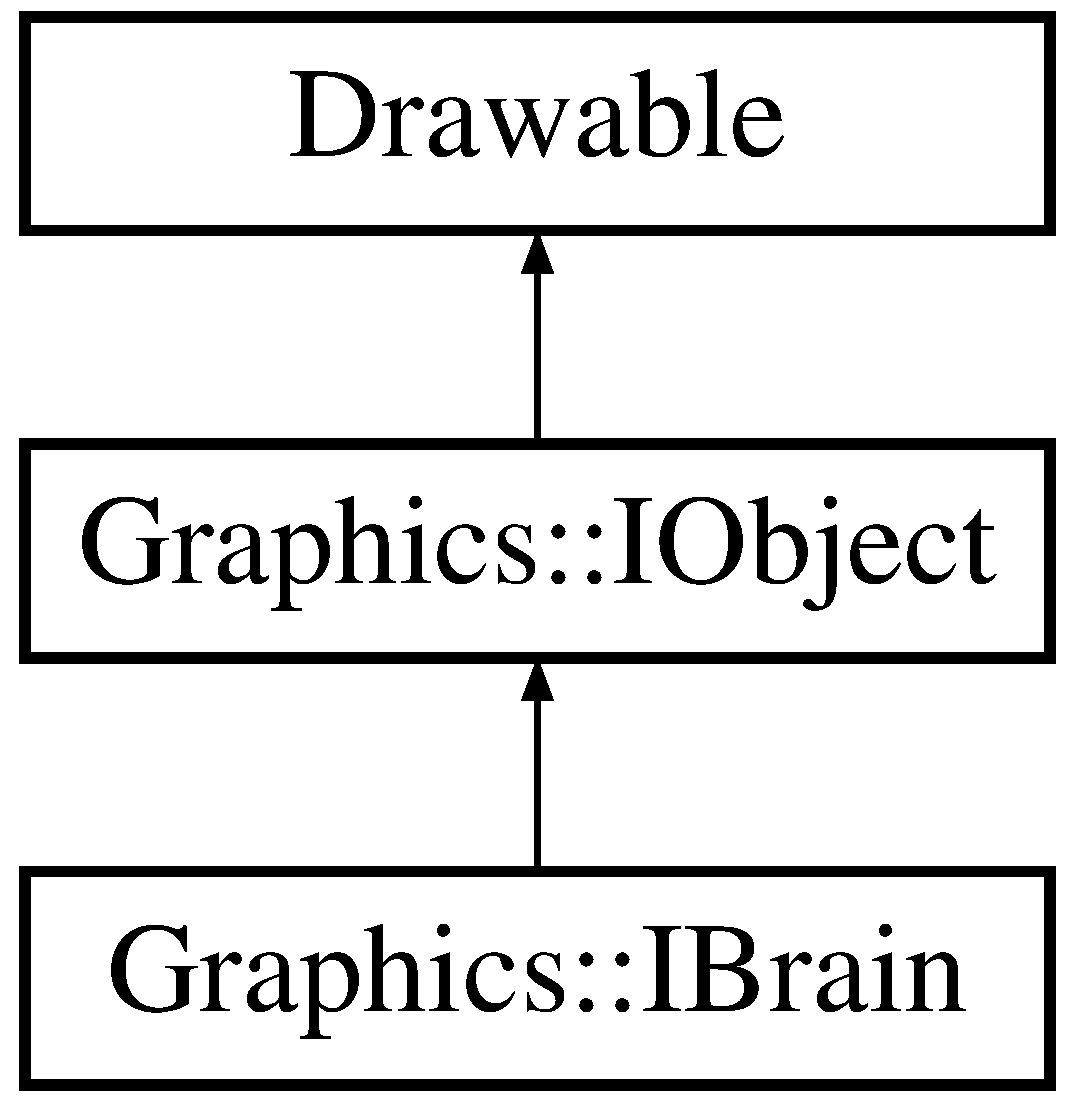
\includegraphics[height=4.000000cm]{class_graphics_1_1_i_object}
\end{center}
\end{figure}
\subsection*{Public Member Functions}
\begin{DoxyCompactItemize}
\item 
virtual bool {\bfseries is\+Dead} (void) const  =0\label{class_graphics_1_1_i_object_a8efbdb791e3a99d697e5c74a1531d2c8}

\item 
virtual bool {\bfseries has\+Brain} (void) const  =0\label{class_graphics_1_1_i_object_a2915106368247427dcff04c5eec2190c}

\item 
virtual std\+::string {\bfseries get\+Type} (void) const  =0\label{class_graphics_1_1_i_object_a9ca3ca5527c0c565d06396efe80ba243}

\item 
virtual void {\bfseries set\+Position} (sf\+::\+Vector2f const \&position)=0\label{class_graphics_1_1_i_object_acb10bc8924396f1e9a8aa510e96ec0c2}

\item 
virtual void {\bfseries set\+Is\+Dead} (bool condition)=0\label{class_graphics_1_1_i_object_a55f6f70a2c0c2690b6b6a78a75ece3fb}

\item 
virtual void {\bfseries set\+Elapsed\+Time} (sf\+::\+Time \&time)=0\label{class_graphics_1_1_i_object_af8866f1765a721c230556bfa391d0299}

\item 
virtual {\bf I\+Object} $\ast$ {\bfseries Clone} (void)=0\label{class_graphics_1_1_i_object_a1f863b90e0b37e462c487731cc218fdd}

\item 
virtual void {\bfseries Update} (void)=0\label{class_graphics_1_1_i_object_a45b5308a10381dd4f41faeef2d06f46c}

\item 
virtual {\bf $\sim$\+I\+Object} (void)\label{class_graphics_1_1_i_object_a754738cfd4e41113f438a3e0fbed8e08}

\begin{DoxyCompactList}\small\item\em Destructor. \end{DoxyCompactList}\item 
virtual bool {\bf is\+Dead} (void) const  =0
\begin{DoxyCompactList}\small\item\em Verify if the object is dead (not be able to draw). \end{DoxyCompactList}\item 
virtual bool {\bf has\+Brain} (void) const  =0
\begin{DoxyCompactList}\small\item\em Verify if the object contains a neural network. \end{DoxyCompactList}\item 
virtual std\+::string {\bf get\+Type} (void) const  =0
\begin{DoxyCompactList}\small\item\em Get the ky (type) of the object in the environment. \end{DoxyCompactList}\item 
virtual void {\bf set\+Position} (sf\+::\+Vector2f const \&position)=0
\begin{DoxyCompactList}\small\item\em Set the current position of the object. \end{DoxyCompactList}\item 
virtual void {\bf set\+Is\+Dead} (bool condition)=0
\begin{DoxyCompactList}\small\item\em Set the current state of the object. \end{DoxyCompactList}\item 
virtual void {\bf set\+Elapsed\+Time} (sf\+::\+Time \&time)=0
\begin{DoxyCompactList}\small\item\em Set the elapsed time between the previous and the current update. \end{DoxyCompactList}\item 
virtual {\bf I\+Object} $\ast$ {\bf Clone} (void)=0
\begin{DoxyCompactList}\small\item\em Clone the current object. \end{DoxyCompactList}\item 
virtual void {\bf Update} (void)=0\label{class_graphics_1_1_i_object_a45b5308a10381dd4f41faeef2d06f46c}

\begin{DoxyCompactList}\small\item\em Update the object. \end{DoxyCompactList}\item 
virtual bool {\bfseries is\+Dead} (void) const  =0\label{class_graphics_1_1_i_object_a8efbdb791e3a99d697e5c74a1531d2c8}

\item 
virtual bool {\bfseries has\+Brain} (void) const  =0\label{class_graphics_1_1_i_object_a2915106368247427dcff04c5eec2190c}

\item 
virtual std\+::string {\bfseries get\+Type} (void) const  =0\label{class_graphics_1_1_i_object_a9ca3ca5527c0c565d06396efe80ba243}

\item 
virtual void {\bfseries set\+Position} (sf\+::\+Vector2f const \&position)=0\label{class_graphics_1_1_i_object_acb10bc8924396f1e9a8aa510e96ec0c2}

\item 
virtual void {\bfseries set\+Is\+Dead} (bool condition)=0\label{class_graphics_1_1_i_object_a55f6f70a2c0c2690b6b6a78a75ece3fb}

\item 
virtual void {\bfseries set\+Elapsed\+Time} (sf\+::\+Time \&time)=0\label{class_graphics_1_1_i_object_af8866f1765a721c230556bfa391d0299}

\item 
virtual {\bf I\+Object} $\ast$ {\bfseries Clone} (void)=0\label{class_graphics_1_1_i_object_a1f863b90e0b37e462c487731cc218fdd}

\item 
virtual void {\bfseries Update} (void)=0\label{class_graphics_1_1_i_object_a45b5308a10381dd4f41faeef2d06f46c}

\end{DoxyCompactItemize}
\subsection*{Protected Member Functions}
\begin{DoxyCompactItemize}
\item 
virtual void {\bfseries draw} (sf\+::\+Render\+Target \&target, sf\+::\+Render\+States states) const  =0\label{class_graphics_1_1_i_object_a1bbb236da76f9cff3750afb768be6260}

\item 
virtual void {\bf draw} (sf\+::\+Render\+Target \&target, sf\+::\+Render\+States states) const  =0
\begin{DoxyCompactList}\small\item\em Allow the object to be drawn on the window. \end{DoxyCompactList}\item 
virtual void {\bfseries draw} (sf\+::\+Render\+Target \&target, sf\+::\+Render\+States states) const  =0\label{class_graphics_1_1_i_object_a1bbb236da76f9cff3750afb768be6260}

\end{DoxyCompactItemize}


\subsection{Detailed Description}
Define the interface of an object. 

\subsection{Member Function Documentation}
\index{Graphics\+::\+I\+Object@{Graphics\+::\+I\+Object}!Clone@{Clone}}
\index{Clone@{Clone}!Graphics\+::\+I\+Object@{Graphics\+::\+I\+Object}}
\subsubsection[{Clone(void)=0}]{\setlength{\rightskip}{0pt plus 5cm}virtual {\bf I\+Object}$\ast$ Graphics\+::\+I\+Object\+::\+Clone (
\begin{DoxyParamCaption}
\item[{void}]{}
\end{DoxyParamCaption}
)\hspace{0.3cm}{\ttfamily [pure virtual]}}\label{class_graphics_1_1_i_object_a1f863b90e0b37e462c487731cc218fdd}


Clone the current object. 

\begin{DoxyReturn}{Returns}
success \+: \doxyref{I\+Object}{p.}{class_graphics_1_1_i_object} 

error \+: N\+U\+L\+L 
\end{DoxyReturn}
\index{Graphics\+::\+I\+Object@{Graphics\+::\+I\+Object}!draw@{draw}}
\index{draw@{draw}!Graphics\+::\+I\+Object@{Graphics\+::\+I\+Object}}
\subsubsection[{draw(sf\+::\+Render\+Target \&target, sf\+::\+Render\+States states) const  =0}]{\setlength{\rightskip}{0pt plus 5cm}virtual void Graphics\+::\+I\+Object\+::draw (
\begin{DoxyParamCaption}
\item[{sf\+::\+Render\+Target \&}]{target, }
\item[{sf\+::\+Render\+States}]{states}
\end{DoxyParamCaption}
) const\hspace{0.3cm}{\ttfamily [protected]}, {\ttfamily [pure virtual]}}\label{class_graphics_1_1_i_object_a1bbb236da76f9cff3750afb768be6260}


Allow the object to be drawn on the window. 


\begin{DoxyParams}{Parameters}
{\em target} & \+: Contains the render target. \\
\hline
{\em states} & \+: Contains the current state of the render target. \\
\hline
\end{DoxyParams}
\index{Graphics\+::\+I\+Object@{Graphics\+::\+I\+Object}!get\+Type@{get\+Type}}
\index{get\+Type@{get\+Type}!Graphics\+::\+I\+Object@{Graphics\+::\+I\+Object}}
\subsubsection[{get\+Type(void) const  =0}]{\setlength{\rightskip}{0pt plus 5cm}virtual std\+::string Graphics\+::\+I\+Object\+::get\+Type (
\begin{DoxyParamCaption}
\item[{void}]{}
\end{DoxyParamCaption}
) const\hspace{0.3cm}{\ttfamily [pure virtual]}}\label{class_graphics_1_1_i_object_a9ca3ca5527c0c565d06396efe80ba243}


Get the ky (type) of the object in the environment. 

\begin{DoxyReturn}{Returns}
std\+::string 
\end{DoxyReturn}
\index{Graphics\+::\+I\+Object@{Graphics\+::\+I\+Object}!has\+Brain@{has\+Brain}}
\index{has\+Brain@{has\+Brain}!Graphics\+::\+I\+Object@{Graphics\+::\+I\+Object}}
\subsubsection[{has\+Brain(void) const  =0}]{\setlength{\rightskip}{0pt plus 5cm}virtual bool Graphics\+::\+I\+Object\+::has\+Brain (
\begin{DoxyParamCaption}
\item[{void}]{}
\end{DoxyParamCaption}
) const\hspace{0.3cm}{\ttfamily [pure virtual]}}\label{class_graphics_1_1_i_object_a2915106368247427dcff04c5eec2190c}


Verify if the object contains a neural network. 

\begin{DoxyReturn}{Returns}
true \+: if the object has a neural network. 

false \+: if the object doesn\textquotesingle{}t have not a neural netowrk. 
\end{DoxyReturn}
\index{Graphics\+::\+I\+Object@{Graphics\+::\+I\+Object}!is\+Dead@{is\+Dead}}
\index{is\+Dead@{is\+Dead}!Graphics\+::\+I\+Object@{Graphics\+::\+I\+Object}}
\subsubsection[{is\+Dead(void) const  =0}]{\setlength{\rightskip}{0pt plus 5cm}virtual bool Graphics\+::\+I\+Object\+::is\+Dead (
\begin{DoxyParamCaption}
\item[{void}]{}
\end{DoxyParamCaption}
) const\hspace{0.3cm}{\ttfamily [pure virtual]}}\label{class_graphics_1_1_i_object_a8efbdb791e3a99d697e5c74a1531d2c8}


Verify if the object is dead (not be able to draw). 

\begin{DoxyReturn}{Returns}
true \+: if the object is dead. 

false \+: if the object is not dead. 
\end{DoxyReturn}
\index{Graphics\+::\+I\+Object@{Graphics\+::\+I\+Object}!set\+Elapsed\+Time@{set\+Elapsed\+Time}}
\index{set\+Elapsed\+Time@{set\+Elapsed\+Time}!Graphics\+::\+I\+Object@{Graphics\+::\+I\+Object}}
\subsubsection[{set\+Elapsed\+Time(sf\+::\+Time \&time)=0}]{\setlength{\rightskip}{0pt plus 5cm}virtual void Graphics\+::\+I\+Object\+::set\+Elapsed\+Time (
\begin{DoxyParamCaption}
\item[{sf\+::\+Time \&}]{time}
\end{DoxyParamCaption}
)\hspace{0.3cm}{\ttfamily [pure virtual]}}\label{class_graphics_1_1_i_object_af8866f1765a721c230556bfa391d0299}


Set the elapsed time between the previous and the current update. 


\begin{DoxyParams}{Parameters}
{\em time} & \+: Contains the delta time. \\
\hline
\end{DoxyParams}
\index{Graphics\+::\+I\+Object@{Graphics\+::\+I\+Object}!set\+Is\+Dead@{set\+Is\+Dead}}
\index{set\+Is\+Dead@{set\+Is\+Dead}!Graphics\+::\+I\+Object@{Graphics\+::\+I\+Object}}
\subsubsection[{set\+Is\+Dead(bool condition)=0}]{\setlength{\rightskip}{0pt plus 5cm}virtual void Graphics\+::\+I\+Object\+::set\+Is\+Dead (
\begin{DoxyParamCaption}
\item[{bool}]{condition}
\end{DoxyParamCaption}
)\hspace{0.3cm}{\ttfamily [pure virtual]}}\label{class_graphics_1_1_i_object_a55f6f70a2c0c2690b6b6a78a75ece3fb}


Set the current state of the object. 


\begin{DoxyParams}{Parameters}
{\em condition} & \+: Contains if the object is dead or not. \\
\hline
\end{DoxyParams}
\index{Graphics\+::\+I\+Object@{Graphics\+::\+I\+Object}!set\+Position@{set\+Position}}
\index{set\+Position@{set\+Position}!Graphics\+::\+I\+Object@{Graphics\+::\+I\+Object}}
\subsubsection[{set\+Position(sf\+::\+Vector2f const \&position)=0}]{\setlength{\rightskip}{0pt plus 5cm}virtual void Graphics\+::\+I\+Object\+::set\+Position (
\begin{DoxyParamCaption}
\item[{sf\+::\+Vector2f const \&}]{position}
\end{DoxyParamCaption}
)\hspace{0.3cm}{\ttfamily [pure virtual]}}\label{class_graphics_1_1_i_object_acb10bc8924396f1e9a8aa510e96ec0c2}


Set the current position of the object. 


\begin{DoxyParams}{Parameters}
{\em position} & \+: Contains the new position of the object. \\
\hline
\end{DoxyParams}


The documentation for this class was generated from the following file\+:\begin{DoxyCompactItemize}
\item 
/home/robin\+\_\+f/\+Programming/\+Git/\+C\+P\+P/\+Love\+Brains/api/include/\+Graphics/i\+\_\+object.\+h\end{DoxyCompactItemize}

\section{Plugin\+:\+:I\+Plugin Class Reference}
\label{class_plugin_1_1_i_plugin}\index{Plugin\+::\+I\+Plugin@{Plugin\+::\+I\+Plugin}}


Define the plugin interface in order to add some stuff to Love\+Brains. Mandatory name for the Plugin\+Creator function \+: \char`\"{}\+Create\+Plugin\char`\"{} !  




{\ttfamily \#include $<$i\+\_\+plugin.\+h$>$}

Inheritance diagram for Plugin\+:\+:I\+Plugin\+:\begin{figure}[H]
\begin{center}
\leavevmode
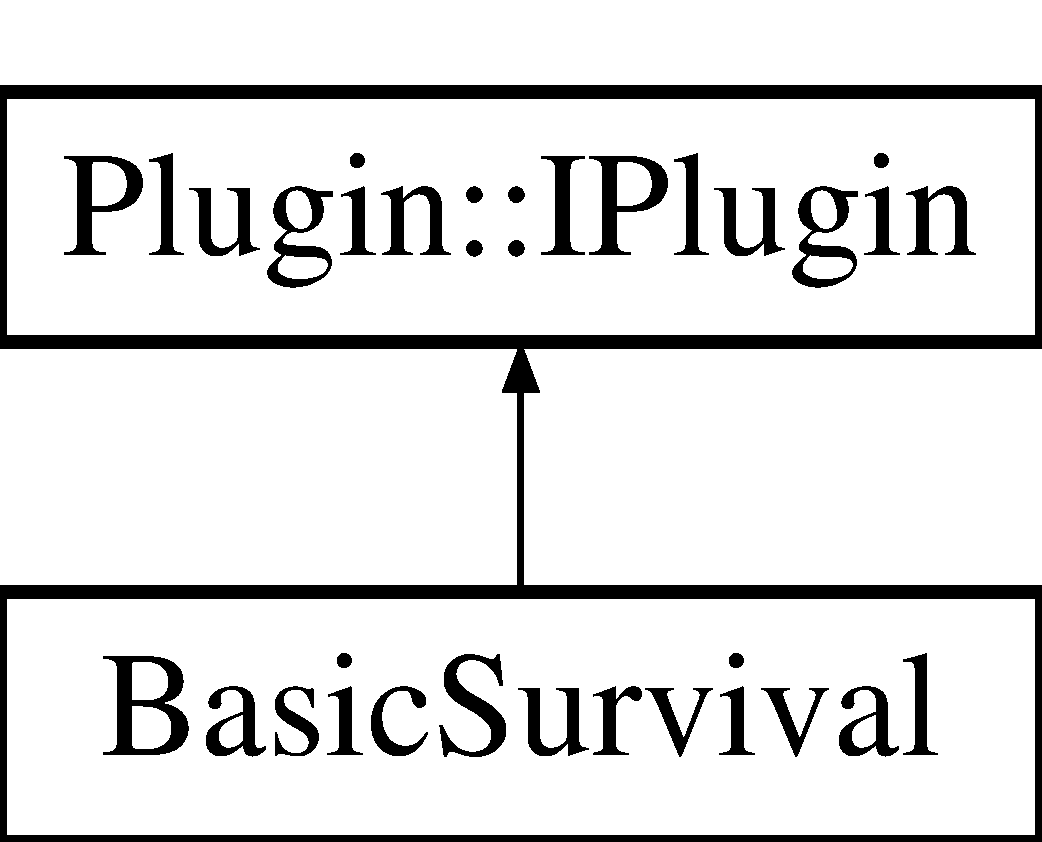
\includegraphics[height=2.000000cm]{class_plugin_1_1_i_plugin}
\end{center}
\end{figure}
\subsection*{Public Types}
\begin{DoxyCompactItemize}
\item 
typedef {\bf I\+Plugin} $\ast$($\ast$ {\bfseries Plugin\+Creator}) (void)\label{class_plugin_1_1_i_plugin_acabdfce5c711ade0685f6d92b3200fd9}

\item 
typedef {\bf I\+Plugin} $\ast$($\ast$ {\bf Plugin\+Creator}) (void)\label{class_plugin_1_1_i_plugin_acabdfce5c711ade0685f6d92b3200fd9}

\begin{DoxyCompactList}\small\item\em Define the function pointer for the creation method. \end{DoxyCompactList}\item 
typedef {\bf I\+Plugin} $\ast$($\ast$ {\bfseries Plugin\+Creator}) (void)\label{class_plugin_1_1_i_plugin_acabdfce5c711ade0685f6d92b3200fd9}

\item 
typedef {\bf I\+Plugin} $\ast$($\ast$ {\bfseries Plugin\+Creator}) (void)\label{class_plugin_1_1_i_plugin_acabdfce5c711ade0685f6d92b3200fd9}

\end{DoxyCompactItemize}
\subsection*{Public Member Functions}
\begin{DoxyCompactItemize}
\item 
virtual std\+::vector$<$ {\bf Graphics\+::\+I\+Object} $\ast$ $>$ \& {\bfseries get\+Objects} (void)=0\label{class_plugin_1_1_i_plugin_a87377dd4f3374d0cfe688af7bda54fc6}

\item 
virtual std\+::vector$<$ {\bf Graphics\+::\+I\+Collider} $\ast$ $>$ \& {\bfseries get\+Colliders} (void)=0\label{class_plugin_1_1_i_plugin_a33a2f401e72044222692bd0dd2f93c3b}

\item 
virtual std\+::vector$<$ {\bf Graphics\+::\+I\+Sensor} $\ast$ $>$ \& {\bfseries get\+Sensors} (void)=0\label{class_plugin_1_1_i_plugin_af37b47e4aeb1b3c457cb58328b83b314}

\item 
virtual {\bf $\sim$\+I\+Plugin} (void)\label{class_plugin_1_1_i_plugin_a8eb9b11fde2be5b2aef3aa4a68979319}

\begin{DoxyCompactList}\small\item\em Virtual destructor. \end{DoxyCompactList}\item 
virtual std\+::vector$<$ {\bf Graphics\+::\+I\+Object} $\ast$ $>$ \& {\bf get\+Objects} (void)=0
\begin{DoxyCompactList}\small\item\em Get all the objects contained by the plugin. \end{DoxyCompactList}\item 
virtual std\+::vector$<$ {\bf Graphics\+::\+I\+Collider} $\ast$ $>$ \& {\bf get\+Colliders} (void)=0
\begin{DoxyCompactList}\small\item\em Get all the colliders contained by the plugin. \end{DoxyCompactList}\item 
virtual std\+::vector$<$ {\bf Graphics\+::\+I\+Sensor} $\ast$ $>$ \& {\bf get\+Sensors} (void)=0
\begin{DoxyCompactList}\small\item\em Get all the sensors contained by the plugin. \end{DoxyCompactList}\item 
virtual std\+::vector$<$ {\bf Graphics\+::\+I\+Object} $\ast$ $>$ \& {\bfseries get\+Objects} (void)=0\label{class_plugin_1_1_i_plugin_a87377dd4f3374d0cfe688af7bda54fc6}

\item 
virtual std\+::vector$<$ {\bf Graphics\+::\+I\+Collider} $\ast$ $>$ \& {\bfseries get\+Colliders} (void)=0\label{class_plugin_1_1_i_plugin_a33a2f401e72044222692bd0dd2f93c3b}

\item 
virtual std\+::vector$<$ {\bf Graphics\+::\+I\+Sensor} $\ast$ $>$ \& {\bfseries get\+Sensors} (void)=0\label{class_plugin_1_1_i_plugin_af37b47e4aeb1b3c457cb58328b83b314}

\item 
virtual std\+::vector$<$ {\bf Graphics\+::\+I\+Object} $\ast$ $>$ \& {\bfseries get\+Objects} (void)=0\label{class_plugin_1_1_i_plugin_a87377dd4f3374d0cfe688af7bda54fc6}

\item 
virtual std\+::vector$<$ {\bf Graphics\+::\+I\+Collider} $\ast$ $>$ \& {\bfseries get\+Colliders} (void)=0\label{class_plugin_1_1_i_plugin_a33a2f401e72044222692bd0dd2f93c3b}

\item 
virtual std\+::vector$<$ {\bf Graphics\+::\+I\+Sensor} $\ast$ $>$ \& {\bfseries get\+Sensors} (void)=0\label{class_plugin_1_1_i_plugin_af37b47e4aeb1b3c457cb58328b83b314}

\end{DoxyCompactItemize}


\subsection{Detailed Description}
Define the plugin interface in order to add some stuff to Love\+Brains. Mandatory name for the Plugin\+Creator function \+: \char`\"{}\+Create\+Plugin\char`\"{} ! 

\subsection{Member Function Documentation}
\index{Plugin\+::\+I\+Plugin@{Plugin\+::\+I\+Plugin}!get\+Colliders@{get\+Colliders}}
\index{get\+Colliders@{get\+Colliders}!Plugin\+::\+I\+Plugin@{Plugin\+::\+I\+Plugin}}
\subsubsection[{get\+Colliders(void)=0}]{\setlength{\rightskip}{0pt plus 5cm}virtual std\+::vector$<${\bf Graphics\+::\+I\+Collider} $\ast$$>$\& Plugin\+::\+I\+Plugin\+::get\+Colliders (
\begin{DoxyParamCaption}
\item[{void}]{}
\end{DoxyParamCaption}
)\hspace{0.3cm}{\ttfamily [pure virtual]}}\label{class_plugin_1_1_i_plugin_a33a2f401e72044222692bd0dd2f93c3b}


Get all the colliders contained by the plugin. 

\begin{DoxyReturn}{Returns}
std\+::vector$<$\+Graphics\+::\+I\+Collider $\ast$$>$\& 
\end{DoxyReturn}
\index{Plugin\+::\+I\+Plugin@{Plugin\+::\+I\+Plugin}!get\+Objects@{get\+Objects}}
\index{get\+Objects@{get\+Objects}!Plugin\+::\+I\+Plugin@{Plugin\+::\+I\+Plugin}}
\subsubsection[{get\+Objects(void)=0}]{\setlength{\rightskip}{0pt plus 5cm}virtual std\+::vector$<${\bf Graphics\+::\+I\+Object} $\ast$$>$\& Plugin\+::\+I\+Plugin\+::get\+Objects (
\begin{DoxyParamCaption}
\item[{void}]{}
\end{DoxyParamCaption}
)\hspace{0.3cm}{\ttfamily [pure virtual]}}\label{class_plugin_1_1_i_plugin_a87377dd4f3374d0cfe688af7bda54fc6}


Get all the objects contained by the plugin. 

\begin{DoxyReturn}{Returns}
std\+::vector$<$\+Graphics\+::\+I\+Object $\ast$$>$\& 
\end{DoxyReturn}
\index{Plugin\+::\+I\+Plugin@{Plugin\+::\+I\+Plugin}!get\+Sensors@{get\+Sensors}}
\index{get\+Sensors@{get\+Sensors}!Plugin\+::\+I\+Plugin@{Plugin\+::\+I\+Plugin}}
\subsubsection[{get\+Sensors(void)=0}]{\setlength{\rightskip}{0pt plus 5cm}virtual std\+::vector$<${\bf Graphics\+::\+I\+Sensor} $\ast$$>$\& Plugin\+::\+I\+Plugin\+::get\+Sensors (
\begin{DoxyParamCaption}
\item[{void}]{}
\end{DoxyParamCaption}
)\hspace{0.3cm}{\ttfamily [pure virtual]}}\label{class_plugin_1_1_i_plugin_af37b47e4aeb1b3c457cb58328b83b314}


Get all the sensors contained by the plugin. 

\begin{DoxyReturn}{Returns}
std\+::vector$<$\+Graphics\+::\+I\+Sensor $\ast$$>$\& 
\end{DoxyReturn}


The documentation for this class was generated from the following file\+:\begin{DoxyCompactItemize}
\item 
api/include/\+Plugin/i\+\_\+plugin.\+h\end{DoxyCompactItemize}

\section{Graphics\+:\+:I\+Sensor Class Reference}
\label{class_graphics_1_1_i_sensor}\index{Graphics\+::\+I\+Sensor@{Graphics\+::\+I\+Sensor}}


Define the interface of a sensor.  




{\ttfamily \#include $<$i\+\_\+sensor.\+h$>$}

Inheritance diagram for Graphics\+:\+:I\+Sensor\+:\begin{figure}[H]
\begin{center}
\leavevmode
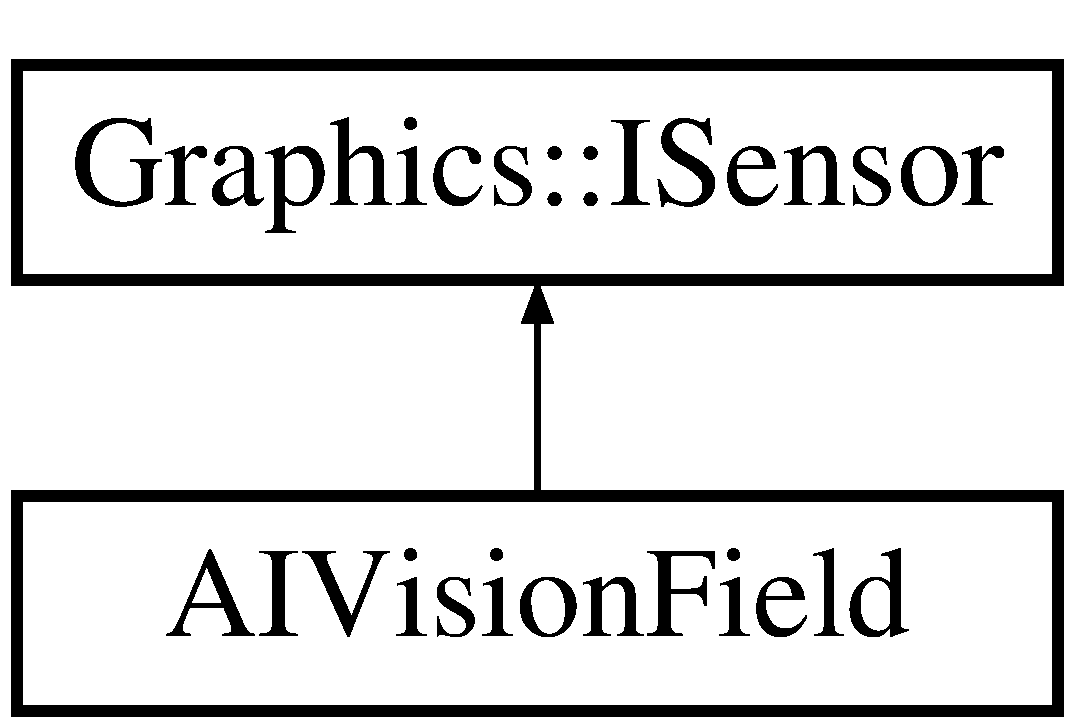
\includegraphics[height=2.000000cm]{class_graphics_1_1_i_sensor}
\end{center}
\end{figure}
\subsection*{Public Member Functions}
\begin{DoxyCompactItemize}
\item 
virtual void {\bfseries Update} ({\bf I\+Object} $\ast$obj, std\+::list$<$ {\bf I\+Object} $\ast$ $>$ \&env)=0\label{class_graphics_1_1_i_sensor_a898b379aa5b3c1e3bd0123a321b2c68a}

\item 
virtual bool {\bfseries is\+Valid} ({\bf I\+Object} $\ast$obj)=0\label{class_graphics_1_1_i_sensor_a7bfe9af666729794a423231e2d91c7c4}

\item 
virtual {\bf $\sim$\+I\+Sensor} ()\label{class_graphics_1_1_i_sensor_a48b21797770f8ab82091f5dac6fb77f1}

\begin{DoxyCompactList}\small\item\em Destructor. \end{DoxyCompactList}\item 
virtual void {\bf Update} ({\bf I\+Object} $\ast$obj, std\+::list$<$ {\bf I\+Object} $\ast$ $>$ \&env)=0
\begin{DoxyCompactList}\small\item\em Update the object in terms of the environment. \end{DoxyCompactList}\item 
virtual bool {\bf is\+Valid} ({\bf I\+Object} $\ast$obj)=0
\begin{DoxyCompactList}\small\item\em Verify if the sensor support the current object. \end{DoxyCompactList}\item 
virtual void {\bfseries Update} ({\bf I\+Object} $\ast$obj, std\+::list$<$ {\bf I\+Object} $\ast$ $>$ \&env)=0\label{class_graphics_1_1_i_sensor_a898b379aa5b3c1e3bd0123a321b2c68a}

\item 
virtual bool {\bfseries is\+Valid} ({\bf I\+Object} $\ast$obj)=0\label{class_graphics_1_1_i_sensor_a7bfe9af666729794a423231e2d91c7c4}

\end{DoxyCompactItemize}


\subsection{Detailed Description}
Define the interface of a sensor. 

\subsection{Member Function Documentation}
\index{Graphics\+::\+I\+Sensor@{Graphics\+::\+I\+Sensor}!is\+Valid@{is\+Valid}}
\index{is\+Valid@{is\+Valid}!Graphics\+::\+I\+Sensor@{Graphics\+::\+I\+Sensor}}
\subsubsection[{is\+Valid(\+I\+Object $\ast$obj)=0}]{\setlength{\rightskip}{0pt plus 5cm}virtual bool Graphics\+::\+I\+Sensor\+::is\+Valid (
\begin{DoxyParamCaption}
\item[{{\bf I\+Object} $\ast$}]{obj}
\end{DoxyParamCaption}
)\hspace{0.3cm}{\ttfamily [pure virtual]}}\label{class_graphics_1_1_i_sensor_a7bfe9af666729794a423231e2d91c7c4}


Verify if the sensor support the current object. 


\begin{DoxyParams}{Parameters}
{\em obj} & \+: Contains the current object. \\
\hline
\end{DoxyParams}
\begin{DoxyReturn}{Returns}
true \+: if the object is supported. 

false \+: if the object is not supported. 
\end{DoxyReturn}
\index{Graphics\+::\+I\+Sensor@{Graphics\+::\+I\+Sensor}!Update@{Update}}
\index{Update@{Update}!Graphics\+::\+I\+Sensor@{Graphics\+::\+I\+Sensor}}
\subsubsection[{Update(\+I\+Object $\ast$obj, std\+::list$<$ I\+Object $\ast$ $>$ \&env)=0}]{\setlength{\rightskip}{0pt plus 5cm}virtual void Graphics\+::\+I\+Sensor\+::\+Update (
\begin{DoxyParamCaption}
\item[{{\bf I\+Object} $\ast$}]{obj, }
\item[{std\+::list$<$ {\bf I\+Object} $\ast$ $>$ \&}]{env}
\end{DoxyParamCaption}
)\hspace{0.3cm}{\ttfamily [pure virtual]}}\label{class_graphics_1_1_i_sensor_a898b379aa5b3c1e3bd0123a321b2c68a}


Update the object in terms of the environment. 


\begin{DoxyParams}{Parameters}
{\em obj} & \+: Contains the object that is involved by the sensor. \\
\hline
{\em env} & \+: Contains all the objects in the environment. \\
\hline
\end{DoxyParams}


The documentation for this class was generated from the following file\+:\begin{DoxyCompactItemize}
\item 
/home/robin\+\_\+f/\+Programming/\+Git/\+C\+P\+P/\+Love\+Brains/api/include/\+Graphics/i\+\_\+sensor.\+h\end{DoxyCompactItemize}

\section{Json\+:\+:Logic\+Error Class Reference}
\label{class_json_1_1_logic_error}\index{Json\+::\+Logic\+Error@{Json\+::\+Logic\+Error}}


{\ttfamily \#include $<$json.\+h$>$}

Inheritance diagram for Json\+:\+:Logic\+Error\+:\begin{figure}[H]
\begin{center}
\leavevmode
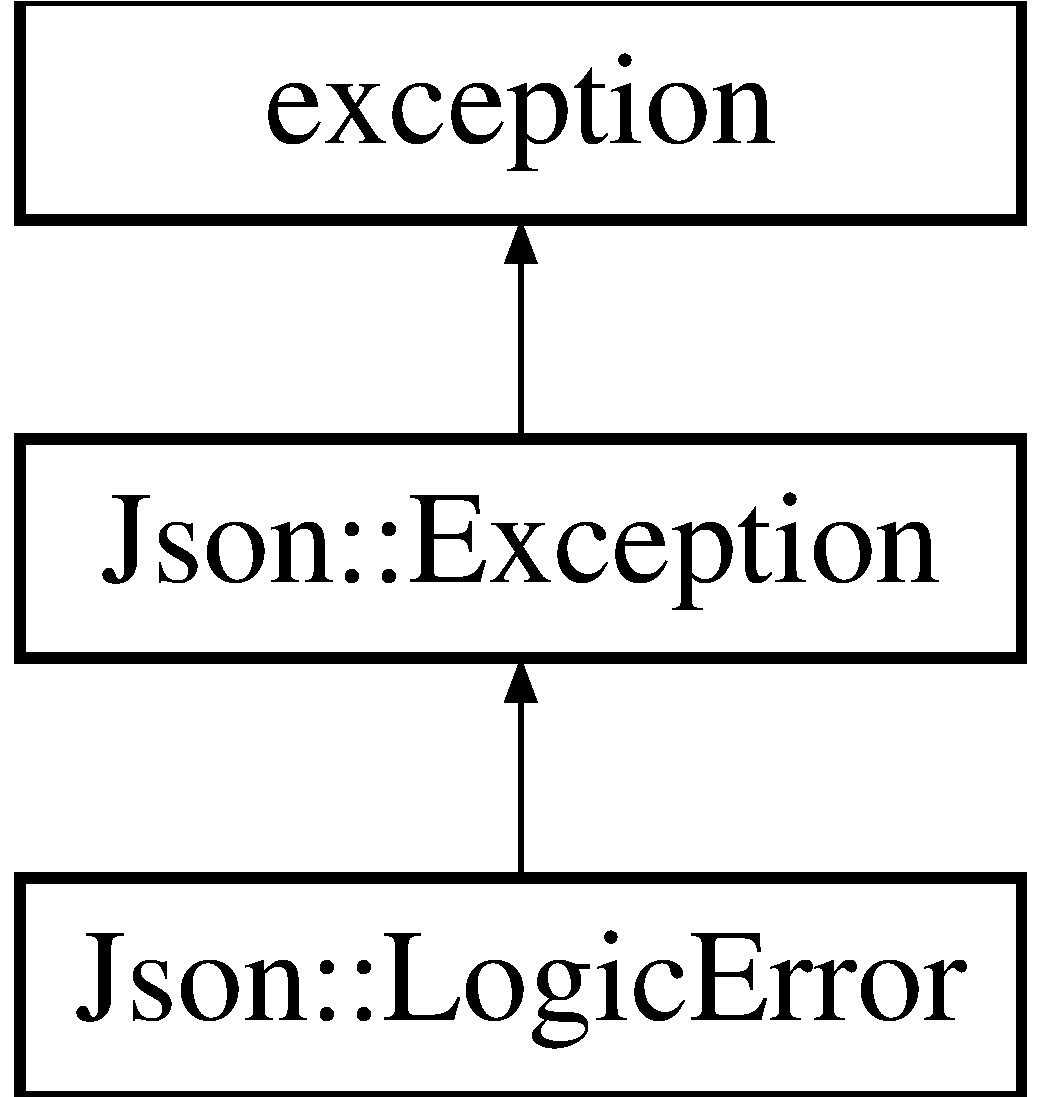
\includegraphics[height=3.684211cm]{class_json_1_1_logic_error}
\end{center}
\end{figure}
\subsection*{Public Member Functions}
\begin{DoxyCompactItemize}
\item 
{\bfseries Logic\+Error} (std\+::string const \&msg)\label{class_json_1_1_logic_error_ae8a834c790017a55df74c70b91f23329}

\item 
{\bfseries Logic\+Error} (std\+::string const \&msg)\label{class_json_1_1_logic_error_ae8a834c790017a55df74c70b91f23329}

\item 
{\bfseries Logic\+Error} (std\+::string const \&msg)\label{class_json_1_1_logic_error_ae8a834c790017a55df74c70b91f23329}

\item 
{\bfseries Logic\+Error} (std\+::string const \&msg)\label{class_json_1_1_logic_error_ae8a834c790017a55df74c70b91f23329}

\end{DoxyCompactItemize}
\subsection*{Additional Inherited Members}


\subsection{Detailed Description}
Exceptions thrown by J\+S\+O\+N\+\_\+\+A\+S\+S\+E\+R\+T/\+J\+S\+O\+N\+\_\+\+F\+A\+I\+L macros.

These are precondition-\/violations (user bugs) and internal errors (our bugs).

\begin{DoxyRemark}{Remarks}
derived from \doxyref{Json\+::\+Exception}{p.}{class_json_1_1_exception} 
\end{DoxyRemark}


The documentation for this class was generated from the following files\+:\begin{DoxyCompactItemize}
\item 
/home/robin\+\_\+f/\+Programming/\+Git/\+C\+P\+P/\+Love\+Brains/api/lib/\+A\+N\+N\+Library/include/json/json.\+h\item 
/home/robin\+\_\+f/\+Programming/\+Git/\+C\+P\+P/\+Love\+Brains/api/lib/\+A\+N\+N\+Library/src/json/jsoncpp.\+cc\end{DoxyCompactItemize}

\section{G\+A\+N\+N\+:\+:Matrix$<$ T $>$ Class Template Reference}
\label{class_g_a_n_n_1_1_matrix}\index{G\+A\+N\+N\+::\+Matrix$<$ T $>$@{G\+A\+N\+N\+::\+Matrix$<$ T $>$}}
\subsection*{Public Member Functions}
\begin{DoxyCompactItemize}
\item 
{\bfseries Matrix} (unsigned int rows, unsigned int cols, T const \&elem)\label{class_g_a_n_n_1_1_matrix_a370ad3ace72e48cf5ac3d2fd672dd679}

\item 
{\bfseries Matrix} ({\bf Matrix} const \&copy)\label{class_g_a_n_n_1_1_matrix_a9af1de05104cf864d0089575e772b74b}

\item 
unsigned int {\bfseries rows} (void) const \label{class_g_a_n_n_1_1_matrix_a14c1233ee25f1cd5823676277e1956f2}

\item 
unsigned int {\bfseries cols} (void) const \label{class_g_a_n_n_1_1_matrix_adc449f757249fe5bfc5bdae3c809d7e7}

\item 
T const \& {\bfseries init} (void) const \label{class_g_a_n_n_1_1_matrix_a5369d9c2dc7ae6a0941f1aba36f15259}

\item 
{\bf Matrix}$<$ T $>$ {\bfseries identity} (unsigned int size, T const \&null, T const \&id)\label{class_g_a_n_n_1_1_matrix_ae61ef07a101463ad49ab8f9f7dd4f2fe}

\item 
{\bf Matrix}$<$ T $>$ \& {\bfseries operator=} ({\bf Matrix}$<$ T $>$ const \&m)\label{class_g_a_n_n_1_1_matrix_a0aa93d1a66567637deb98c943f936fd4}

\item 
const T \& {\bfseries operator[$\,$]} (unsigned int i) const \label{class_g_a_n_n_1_1_matrix_add9f200cb6a2e53709090621e3a1150a}

\item 
T \& {\bfseries operator[$\,$]} (unsigned int i)\label{class_g_a_n_n_1_1_matrix_a700ad2c1e9ab4fd76fe1cb18092a80f1}

\item 
const T \& {\bfseries operator()} (unsigned int i, unsigned int j) const \label{class_g_a_n_n_1_1_matrix_aa3bef5292a718f45e094926602ff65ca}

\item 
T \& {\bfseries operator()} (unsigned int i, unsigned int j)\label{class_g_a_n_n_1_1_matrix_ac3f7f2d7467ba5bc95fca1890be74a38}

\item 
{\bfseries Matrix} (unsigned int rows, unsigned int cols, T const \&elem)\label{class_g_a_n_n_1_1_matrix_a370ad3ace72e48cf5ac3d2fd672dd679}

\item 
{\bfseries Matrix} ({\bf Matrix} const \&copy)\label{class_g_a_n_n_1_1_matrix_a9af1de05104cf864d0089575e772b74b}

\item 
unsigned int {\bfseries rows} (void) const \label{class_g_a_n_n_1_1_matrix_a14c1233ee25f1cd5823676277e1956f2}

\item 
unsigned int {\bfseries cols} (void) const \label{class_g_a_n_n_1_1_matrix_adc449f757249fe5bfc5bdae3c809d7e7}

\item 
T const \& {\bfseries init} (void) const \label{class_g_a_n_n_1_1_matrix_a5369d9c2dc7ae6a0941f1aba36f15259}

\item 
{\bf Matrix}$<$ T $>$ {\bfseries identity} (unsigned int size, T const \&null, T const \&id)\label{class_g_a_n_n_1_1_matrix_ae61ef07a101463ad49ab8f9f7dd4f2fe}

\item 
{\bf Matrix}$<$ T $>$ \& {\bfseries operator=} ({\bf Matrix}$<$ T $>$ const \&m)\label{class_g_a_n_n_1_1_matrix_a0aa93d1a66567637deb98c943f936fd4}

\item 
const T \& {\bfseries operator[$\,$]} (unsigned int i) const \label{class_g_a_n_n_1_1_matrix_add9f200cb6a2e53709090621e3a1150a}

\item 
T \& {\bfseries operator[$\,$]} (unsigned int i)\label{class_g_a_n_n_1_1_matrix_a700ad2c1e9ab4fd76fe1cb18092a80f1}

\item 
const T \& {\bfseries operator()} (unsigned int i, unsigned int j) const \label{class_g_a_n_n_1_1_matrix_aa3bef5292a718f45e094926602ff65ca}

\item 
T \& {\bfseries operator()} (unsigned int i, unsigned int j)\label{class_g_a_n_n_1_1_matrix_ac3f7f2d7467ba5bc95fca1890be74a38}

\end{DoxyCompactItemize}


The documentation for this class was generated from the following file\+:\begin{DoxyCompactItemize}
\item 
/home/robin\+\_\+f/\+Programming/\+Git/\+C\+P\+P/\+Love\+Brains/include/\+A\+N\+N/matrix.\+h\end{DoxyCompactItemize}

\section{Json\+:\+:Our\+Char\+Reader Class Reference}
\label{class_json_1_1_our_char_reader}\index{Json\+::\+Our\+Char\+Reader@{Json\+::\+Our\+Char\+Reader}}
Inheritance diagram for Json\+:\+:Our\+Char\+Reader\+:\begin{figure}[H]
\begin{center}
\leavevmode
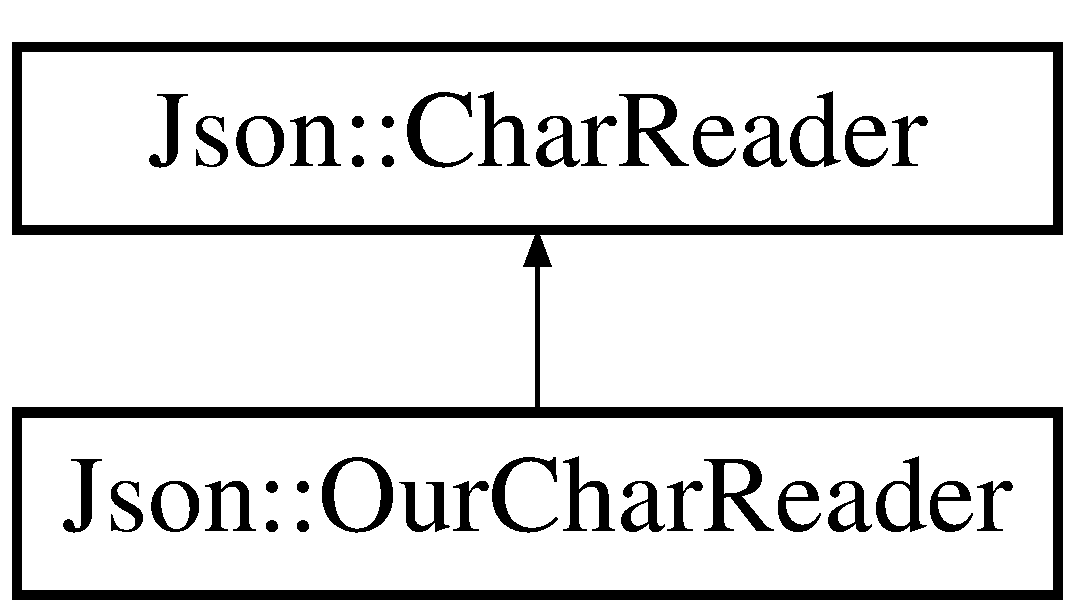
\includegraphics[height=2.000000cm]{class_json_1_1_our_char_reader}
\end{center}
\end{figure}
\subsection*{Public Member Functions}
\begin{DoxyCompactItemize}
\item 
{\bfseries Our\+Char\+Reader} (bool collect\+Comments, {\bf Our\+Features} const \&features)\label{class_json_1_1_our_char_reader_a5015506620e7ba7bab417756fa1ca9fe}

\item 
virtual bool {\bf parse} (char const $\ast$begin\+Doc, char const $\ast$end\+Doc, {\bf Value} $\ast$root, std\+::string $\ast$errs)
\begin{DoxyCompactList}\small\item\em Read a \doxyref{Value}{p.}{class_json_1_1_value} from a {\tt J\+S\+O\+N} document. The document must be a U\+T\+F-\/8 encoded string containing the document to read. \end{DoxyCompactList}\item 
{\bfseries Our\+Char\+Reader} (bool collect\+Comments, {\bf Our\+Features} const \&features)\label{class_json_1_1_our_char_reader_a5015506620e7ba7bab417756fa1ca9fe}

\item 
virtual bool {\bf parse} (char const $\ast$begin\+Doc, char const $\ast$end\+Doc, {\bf Value} $\ast$root, std\+::string $\ast$errs)
\begin{DoxyCompactList}\small\item\em Read a \doxyref{Value}{p.}{class_json_1_1_value} from a {\tt J\+S\+O\+N} document. The document must be a U\+T\+F-\/8 encoded string containing the document to read. \end{DoxyCompactList}\item 
{\bfseries Our\+Char\+Reader} (bool collect\+Comments, {\bf Our\+Features} const \&features)\label{class_json_1_1_our_char_reader_a5015506620e7ba7bab417756fa1ca9fe}

\item 
virtual bool {\bf parse} (char const $\ast$begin\+Doc, char const $\ast$end\+Doc, {\bf Value} $\ast$root, std\+::string $\ast$errs)
\begin{DoxyCompactList}\small\item\em Read a \doxyref{Value}{p.}{class_json_1_1_value} from a {\tt J\+S\+O\+N} document. The document must be a U\+T\+F-\/8 encoded string containing the document to read. \end{DoxyCompactList}\end{DoxyCompactItemize}


\subsection{Member Function Documentation}
\index{Json\+::\+Our\+Char\+Reader@{Json\+::\+Our\+Char\+Reader}!parse@{parse}}
\index{parse@{parse}!Json\+::\+Our\+Char\+Reader@{Json\+::\+Our\+Char\+Reader}}
\subsubsection[{parse(char const $\ast$begin\+Doc, char const $\ast$end\+Doc, Value $\ast$root, std\+::string $\ast$errs)}]{\setlength{\rightskip}{0pt plus 5cm}virtual bool Json\+::\+Our\+Char\+Reader\+::parse (
\begin{DoxyParamCaption}
\item[{char const $\ast$}]{begin\+Doc, }
\item[{char const $\ast$}]{end\+Doc, }
\item[{{\bf Value} $\ast$}]{root, }
\item[{std\+::string $\ast$}]{errs}
\end{DoxyParamCaption}
)\hspace{0.3cm}{\ttfamily [inline]}, {\ttfamily [virtual]}}\label{class_json_1_1_our_char_reader_aa4dce03aee1c111679813133c29f4465}


Read a \doxyref{Value}{p.}{class_json_1_1_value} from a {\tt J\+S\+O\+N} document. The document must be a U\+T\+F-\/8 encoded string containing the document to read. 


\begin{DoxyParams}{Parameters}
{\em begin\+Doc} & Pointer on the beginning of the U\+T\+F-\/8 encoded string of the document to read. \\
\hline
{\em end\+Doc} & Pointer on the end of the U\+T\+F-\/8 encoded string of the document to read. Must be $>$= begin\+Doc. \\
\hline
{\em root} & [out] Contains the root value of the document if it was successfully parsed. \\
\hline
{\em errs} & [out] Formatted error messages (if not N\+U\+L\+L) a user friendly string that lists errors in the parsed document. \\
\hline
\end{DoxyParams}
\begin{DoxyReturn}{Returns}
{\ttfamily true} if the document was successfully parsed, {\ttfamily false} if an error occurred. 
\end{DoxyReturn}


Implements {\bf Json\+::\+Char\+Reader} \doxyref{}{p.}{class_json_1_1_char_reader_a48e320be8b13bbc0960cc5808cafec98}.

\index{Json\+::\+Our\+Char\+Reader@{Json\+::\+Our\+Char\+Reader}!parse@{parse}}
\index{parse@{parse}!Json\+::\+Our\+Char\+Reader@{Json\+::\+Our\+Char\+Reader}}
\subsubsection[{parse(char const $\ast$begin\+Doc, char const $\ast$end\+Doc, Value $\ast$root, std\+::string $\ast$errs)}]{\setlength{\rightskip}{0pt plus 5cm}virtual bool Json\+::\+Our\+Char\+Reader\+::parse (
\begin{DoxyParamCaption}
\item[{char const $\ast$}]{begin\+Doc, }
\item[{char const $\ast$}]{end\+Doc, }
\item[{{\bf Value} $\ast$}]{root, }
\item[{std\+::string $\ast$}]{errs}
\end{DoxyParamCaption}
)\hspace{0.3cm}{\ttfamily [inline]}, {\ttfamily [virtual]}}\label{class_json_1_1_our_char_reader_aa4dce03aee1c111679813133c29f4465}


Read a \doxyref{Value}{p.}{class_json_1_1_value} from a {\tt J\+S\+O\+N} document. The document must be a U\+T\+F-\/8 encoded string containing the document to read. 


\begin{DoxyParams}{Parameters}
{\em begin\+Doc} & Pointer on the beginning of the U\+T\+F-\/8 encoded string of the document to read. \\
\hline
{\em end\+Doc} & Pointer on the end of the U\+T\+F-\/8 encoded string of the document to read. Must be $>$= begin\+Doc. \\
\hline
{\em root} & [out] Contains the root value of the document if it was successfully parsed. \\
\hline
{\em errs} & [out] Formatted error messages (if not N\+U\+L\+L) a user friendly string that lists errors in the parsed document. \\
\hline
\end{DoxyParams}
\begin{DoxyReturn}{Returns}
{\ttfamily true} if the document was successfully parsed, {\ttfamily false} if an error occurred. 
\end{DoxyReturn}


Implements {\bf Json\+::\+Char\+Reader} \doxyref{}{p.}{class_json_1_1_char_reader_a48e320be8b13bbc0960cc5808cafec98}.

\index{Json\+::\+Our\+Char\+Reader@{Json\+::\+Our\+Char\+Reader}!parse@{parse}}
\index{parse@{parse}!Json\+::\+Our\+Char\+Reader@{Json\+::\+Our\+Char\+Reader}}
\subsubsection[{parse(char const $\ast$begin\+Doc, char const $\ast$end\+Doc, Value $\ast$root, std\+::string $\ast$errs)}]{\setlength{\rightskip}{0pt plus 5cm}virtual bool Json\+::\+Our\+Char\+Reader\+::parse (
\begin{DoxyParamCaption}
\item[{char const $\ast$}]{begin\+Doc, }
\item[{char const $\ast$}]{end\+Doc, }
\item[{{\bf Value} $\ast$}]{root, }
\item[{std\+::string $\ast$}]{errs}
\end{DoxyParamCaption}
)\hspace{0.3cm}{\ttfamily [inline]}, {\ttfamily [virtual]}}\label{class_json_1_1_our_char_reader_aa4dce03aee1c111679813133c29f4465}


Read a \doxyref{Value}{p.}{class_json_1_1_value} from a {\tt J\+S\+O\+N} document. The document must be a U\+T\+F-\/8 encoded string containing the document to read. 


\begin{DoxyParams}{Parameters}
{\em begin\+Doc} & Pointer on the beginning of the U\+T\+F-\/8 encoded string of the document to read. \\
\hline
{\em end\+Doc} & Pointer on the end of the U\+T\+F-\/8 encoded string of the document to read. Must be $>$= begin\+Doc. \\
\hline
{\em root} & [out] Contains the root value of the document if it was successfully parsed. \\
\hline
{\em errs} & [out] Formatted error messages (if not N\+U\+L\+L) a user friendly string that lists errors in the parsed document. \\
\hline
\end{DoxyParams}
\begin{DoxyReturn}{Returns}
{\ttfamily true} if the document was successfully parsed, {\ttfamily false} if an error occurred. 
\end{DoxyReturn}


Implements {\bf Json\+::\+Char\+Reader} \doxyref{}{p.}{class_json_1_1_char_reader_a48e320be8b13bbc0960cc5808cafec98}.



The documentation for this class was generated from the following file\+:\begin{DoxyCompactItemize}
\item 
/home/robin\+\_\+f/\+Programming/\+Git/\+C\+P\+P/\+Love\+Brains/api/lib/\+A\+N\+N\+Library/src/json/jsoncpp.\+cc\end{DoxyCompactItemize}

\hypertarget{class_json_1_1_our_features}{}\section{Json\+:\+:Our\+Features Class Reference}
\label{class_json_1_1_our_features}\index{Json\+::\+Our\+Features@{Json\+::\+Our\+Features}}
\subsection*{Static Public Member Functions}
\begin{DoxyCompactItemize}
\item 
\hypertarget{class_json_1_1_our_features_a0686e1406b6677f496529f9f3fe98d1e}{}static \hyperlink{class_json_1_1_our_features}{Our\+Features} {\bfseries all} ()\label{class_json_1_1_our_features_a0686e1406b6677f496529f9f3fe98d1e}

\end{DoxyCompactItemize}
\subsection*{Public Attributes}
\begin{DoxyCompactItemize}
\item 
\hypertarget{class_json_1_1_our_features_ac71bb7ba7363d3b05ed76602b036ce33}{}bool {\bfseries allow\+Comments\+\_\+}\label{class_json_1_1_our_features_ac71bb7ba7363d3b05ed76602b036ce33}

\item 
\hypertarget{class_json_1_1_our_features_a2095f66a776c0a4ae6cc931a0c94242e}{}bool {\bfseries strict\+Root\+\_\+}\label{class_json_1_1_our_features_a2095f66a776c0a4ae6cc931a0c94242e}

\item 
\hypertarget{class_json_1_1_our_features_a13963bc44bf948eec1968f7ff8e8f5f1}{}bool {\bfseries allow\+Dropped\+Null\+Placeholders\+\_\+}\label{class_json_1_1_our_features_a13963bc44bf948eec1968f7ff8e8f5f1}

\item 
\hypertarget{class_json_1_1_our_features_af6973fc7e774ce2d634ba99442aeb91a}{}bool {\bfseries allow\+Numeric\+Keys\+\_\+}\label{class_json_1_1_our_features_af6973fc7e774ce2d634ba99442aeb91a}

\item 
\hypertarget{class_json_1_1_our_features_abbd6c196d7a22e2a360a59887eda4610}{}bool {\bfseries allow\+Single\+Quotes\+\_\+}\label{class_json_1_1_our_features_abbd6c196d7a22e2a360a59887eda4610}

\item 
\hypertarget{class_json_1_1_our_features_ae8ad25b90706c78f1a8fe929191ac61b}{}bool {\bfseries fail\+If\+Extra\+\_\+}\label{class_json_1_1_our_features_ae8ad25b90706c78f1a8fe929191ac61b}

\item 
\hypertarget{class_json_1_1_our_features_a39b8e0b86b1c24a45e800c023bb715aa}{}bool {\bfseries reject\+Dup\+Keys\+\_\+}\label{class_json_1_1_our_features_a39b8e0b86b1c24a45e800c023bb715aa}

\item 
\hypertarget{class_json_1_1_our_features_a9a786713902d14be6d57a08cc03ccfff}{}int {\bfseries stack\+Limit\+\_\+}\label{class_json_1_1_our_features_a9a786713902d14be6d57a08cc03ccfff}

\end{DoxyCompactItemize}


The documentation for this class was generated from the following file\+:\begin{DoxyCompactItemize}
\item 
/home/robin\+\_\+f/\+Programming/\+Git/\+C\+P\+P/\+Love\+Brains/api/lib/\+A\+N\+N\+Library/src/json/jsoncpp.\+cc\end{DoxyCompactItemize}

\section{Json\+:\+:Our\+Reader Class Reference}
\label{class_json_1_1_our_reader}\index{Json\+::\+Our\+Reader@{Json\+::\+Our\+Reader}}
\subsection*{Classes}
\begin{DoxyCompactItemize}
\item 
struct {\bf Structured\+Error}
\end{DoxyCompactItemize}
\subsection*{Public Types}
\begin{DoxyCompactItemize}
\item 
typedef char {\bfseries Char}\label{class_json_1_1_our_reader_a0cd0bab4caa66594ab843ccd5f9dc239}

\item 
typedef const Char $\ast$ {\bfseries Location}\label{class_json_1_1_our_reader_a1bdc7bbc52ba87cae6b19746f2ee0189}

\item 
typedef char {\bfseries Char}\label{class_json_1_1_our_reader_a0cd0bab4caa66594ab843ccd5f9dc239}

\item 
typedef const Char $\ast$ {\bfseries Location}\label{class_json_1_1_our_reader_a1bdc7bbc52ba87cae6b19746f2ee0189}

\item 
typedef char {\bfseries Char}\label{class_json_1_1_our_reader_a0cd0bab4caa66594ab843ccd5f9dc239}

\item 
typedef const Char $\ast$ {\bfseries Location}\label{class_json_1_1_our_reader_a1bdc7bbc52ba87cae6b19746f2ee0189}

\end{DoxyCompactItemize}
\subsection*{Public Member Functions}
\begin{DoxyCompactItemize}
\item 
{\bfseries Our\+Reader} ({\bf Our\+Features} const \&features)\label{class_json_1_1_our_reader_a48a850914b9c8d7781be172930c478e5}

\item 
bool {\bfseries parse} (const char $\ast$begin\+Doc, const char $\ast$end\+Doc, {\bf Value} \&root, bool collect\+Comments=true)\label{class_json_1_1_our_reader_aba4f8749aab7f02ec17f107e392caf80}

\item 
std\+::string {\bfseries get\+Formatted\+Error\+Messages} () const \label{class_json_1_1_our_reader_ae9cbb7dbd9c6c96be37432e8dfa1afcb}

\item 
std\+::vector$<$ {\bf Structured\+Error} $>$ {\bfseries get\+Structured\+Errors} () const \label{class_json_1_1_our_reader_a02ef7871af3706754a233c36e6d489e9}

\item 
bool {\bfseries push\+Error} (const {\bf Value} \&value, const std\+::string \&message)\label{class_json_1_1_our_reader_aef7aa4ca22ffaa38c401b16951d20e1e}

\item 
bool {\bfseries push\+Error} (const {\bf Value} \&value, const std\+::string \&message, const {\bf Value} \&extra)\label{class_json_1_1_our_reader_ad43315cbb0d6804e3b7177e84a1ec53d}

\item 
bool {\bfseries good} () const \label{class_json_1_1_our_reader_a048346238d703ad9aed06beb686e6102}

\item 
{\bfseries Our\+Reader} ({\bf Our\+Features} const \&features)\label{class_json_1_1_our_reader_a48a850914b9c8d7781be172930c478e5}

\item 
bool {\bfseries parse} (const char $\ast$begin\+Doc, const char $\ast$end\+Doc, {\bf Value} \&root, bool collect\+Comments=true)\label{class_json_1_1_our_reader_aba4f8749aab7f02ec17f107e392caf80}

\item 
std\+::string {\bfseries get\+Formatted\+Error\+Messages} () const \label{class_json_1_1_our_reader_ae9cbb7dbd9c6c96be37432e8dfa1afcb}

\item 
std\+::vector$<$ {\bf Structured\+Error} $>$ {\bfseries get\+Structured\+Errors} () const \label{class_json_1_1_our_reader_a2f7d35771be02703be2d0ac1877bc149}

\item 
bool {\bfseries push\+Error} (const {\bf Value} \&value, const std\+::string \&message)\label{class_json_1_1_our_reader_aef7aa4ca22ffaa38c401b16951d20e1e}

\item 
bool {\bfseries push\+Error} (const {\bf Value} \&value, const std\+::string \&message, const {\bf Value} \&extra)\label{class_json_1_1_our_reader_ad43315cbb0d6804e3b7177e84a1ec53d}

\item 
bool {\bfseries good} () const \label{class_json_1_1_our_reader_a048346238d703ad9aed06beb686e6102}

\item 
{\bfseries Our\+Reader} ({\bf Our\+Features} const \&features)\label{class_json_1_1_our_reader_a48a850914b9c8d7781be172930c478e5}

\item 
bool {\bfseries parse} (const char $\ast$begin\+Doc, const char $\ast$end\+Doc, {\bf Value} \&root, bool collect\+Comments=true)\label{class_json_1_1_our_reader_aba4f8749aab7f02ec17f107e392caf80}

\item 
std\+::string {\bfseries get\+Formatted\+Error\+Messages} () const \label{class_json_1_1_our_reader_ae9cbb7dbd9c6c96be37432e8dfa1afcb}

\item 
std\+::vector$<$ {\bf Structured\+Error} $>$ {\bfseries get\+Structured\+Errors} () const \label{class_json_1_1_our_reader_a2f7d35771be02703be2d0ac1877bc149}

\item 
bool {\bfseries push\+Error} (const {\bf Value} \&value, const std\+::string \&message)\label{class_json_1_1_our_reader_aef7aa4ca22ffaa38c401b16951d20e1e}

\item 
bool {\bfseries push\+Error} (const {\bf Value} \&value, const std\+::string \&message, const {\bf Value} \&extra)\label{class_json_1_1_our_reader_ad43315cbb0d6804e3b7177e84a1ec53d}

\item 
bool {\bfseries good} () const \label{class_json_1_1_our_reader_a048346238d703ad9aed06beb686e6102}

\end{DoxyCompactItemize}


The documentation for this class was generated from the following file\+:\begin{DoxyCompactItemize}
\item 
/home/robin\+\_\+f/\+Programming/\+Git/\+C\+P\+P/\+Love\+Brains/api/lib/\+A\+N\+N\+Library/src/json/jsoncpp.\+cc\end{DoxyCompactItemize}

\hypertarget{class_json_1_1_path}{}\section{Json\+:\+:Path Class Reference}
\label{class_json_1_1_path}\index{Json\+::\+Path@{Json\+::\+Path}}


Experimental and untested\+: represents a \char`\"{}path\char`\"{} to access a node.  




{\ttfamily \#include $<$json.\+h$>$}

\subsection*{Public Member Functions}
\begin{DoxyCompactItemize}
\item 
\hypertarget{class_json_1_1_path_aaa37a99650e770d0cd680bf53585ec99}{}{\bfseries Path} (const std\+::string \&path, const \hyperlink{class_json_1_1_path_argument}{Path\+Argument} \&a1=\hyperlink{class_json_1_1_path_argument}{Path\+Argument}(), const \hyperlink{class_json_1_1_path_argument}{Path\+Argument} \&a2=\hyperlink{class_json_1_1_path_argument}{Path\+Argument}(), const \hyperlink{class_json_1_1_path_argument}{Path\+Argument} \&a3=\hyperlink{class_json_1_1_path_argument}{Path\+Argument}(), const \hyperlink{class_json_1_1_path_argument}{Path\+Argument} \&a4=\hyperlink{class_json_1_1_path_argument}{Path\+Argument}(), const \hyperlink{class_json_1_1_path_argument}{Path\+Argument} \&a5=\hyperlink{class_json_1_1_path_argument}{Path\+Argument}())\label{class_json_1_1_path_aaa37a99650e770d0cd680bf53585ec99}

\item 
\hypertarget{class_json_1_1_path_ae1d05fa985a6ee3c57f2b8ed186b5982}{}const \hyperlink{class_json_1_1_value}{Value} \& {\bfseries resolve} (const \hyperlink{class_json_1_1_value}{Value} \&root) const \label{class_json_1_1_path_ae1d05fa985a6ee3c57f2b8ed186b5982}

\item 
\hypertarget{class_json_1_1_path_a33d1749770a4cf74e9a3de419bc7febe}{}\hyperlink{class_json_1_1_value}{Value} {\bfseries resolve} (const \hyperlink{class_json_1_1_value}{Value} \&root, const \hyperlink{class_json_1_1_value}{Value} \&default\+Value) const \label{class_json_1_1_path_a33d1749770a4cf74e9a3de419bc7febe}

\item 
\hyperlink{class_json_1_1_value}{Value} \& \hyperlink{class_json_1_1_path_a5289901fc58ad1fdca1de7fb5a0b620c}{make} (\hyperlink{class_json_1_1_value}{Value} \&root) const 
\end{DoxyCompactItemize}


\subsection{Detailed Description}
Experimental and untested\+: represents a \char`\"{}path\char`\"{} to access a node. 

Syntax\+:
\begin{DoxyItemize}
\item \char`\"{}.\char`\"{} =$>$ root node
\item \char`\"{}.\mbox{[}n\mbox{]}\char`\"{} =$>$ elements at index \textquotesingle{}n\textquotesingle{} of root node (an array value)
\item \char`\"{}.\+name\char`\"{} =$>$ member named \textquotesingle{}name\textquotesingle{} of root node (an object value)
\item \char`\"{}.\+name1.\+name2.\+name3\char`\"{}
\item \char`\"{}.\mbox{[}0\mbox{]}\mbox{[}1\mbox{]}\mbox{[}2\mbox{]}.\+name1\mbox{[}3\mbox{]}\char`\"{}
\item \char`\"{}.\%\char`\"{} =$>$ member name is provided as parameter
\item \char`\"{}.\mbox{[}\%\mbox{]}\char`\"{} =$>$ index is provied as parameter 
\end{DoxyItemize}

\subsection{Member Function Documentation}
\hypertarget{class_json_1_1_path_a5289901fc58ad1fdca1de7fb5a0b620c}{}\index{Json\+::\+Path@{Json\+::\+Path}!make@{make}}
\index{make@{make}!Json\+::\+Path@{Json\+::\+Path}}
\subsubsection[{make(\+Value \&root) const }]{\setlength{\rightskip}{0pt plus 5cm}{\bf Value} \& Json\+::\+Path\+::make (
\begin{DoxyParamCaption}
\item[{{\bf Value} \&}]{root}
\end{DoxyParamCaption}
) const}\label{class_json_1_1_path_a5289901fc58ad1fdca1de7fb5a0b620c}
Creates the \char`\"{}path\char`\"{} to access the specified node and returns a reference on the node. 

The documentation for this class was generated from the following files\+:\begin{DoxyCompactItemize}
\item 
/home/robin\+\_\+f/\+Programming/\+Git/\+C\+P\+P/\+Love\+Brains/api/lib/\+A\+N\+N\+Library/include/json/json.\+h\item 
/home/robin\+\_\+f/\+Programming/\+Git/\+C\+P\+P/\+Love\+Brains/api/lib/\+A\+N\+N\+Library/src/json/jsoncpp.\+cc\end{DoxyCompactItemize}

\section{Json\+:\+:Path\+Argument Class Reference}
\label{class_json_1_1_path_argument}\index{Json\+::\+Path\+Argument@{Json\+::\+Path\+Argument}}


Experimental and untested\+: represents an element of the \char`\"{}path\char`\"{} to access a node.  




{\ttfamily \#include $<$json.\+h$>$}

\subsection*{Public Member Functions}
\begin{DoxyCompactItemize}
\item 
{\bfseries Path\+Argument} (Array\+Index index)\label{class_json_1_1_path_argument_a53c5b27143b161301b95fd544c139ecf}

\item 
{\bfseries Path\+Argument} (const char $\ast$key)\label{class_json_1_1_path_argument_a9690417a8a40e6e49f2acdf6c9281345}

\item 
{\bfseries Path\+Argument} (const std\+::string \&key)\label{class_json_1_1_path_argument_a08f872cfee4fc600f7fa3bcaaff0d41c}

\item 
{\bfseries Path\+Argument} (Array\+Index index)\label{class_json_1_1_path_argument_a53c5b27143b161301b95fd544c139ecf}

\item 
{\bfseries Path\+Argument} (const char $\ast$key)\label{class_json_1_1_path_argument_a9690417a8a40e6e49f2acdf6c9281345}

\item 
{\bfseries Path\+Argument} (const std\+::string \&key)\label{class_json_1_1_path_argument_a08f872cfee4fc600f7fa3bcaaff0d41c}

\end{DoxyCompactItemize}
\subsection*{Friends}
\begin{DoxyCompactItemize}
\item 
class {\bfseries Path}\label{class_json_1_1_path_argument_a51971c24df68e5ad775ed4f8c33e968f}

\end{DoxyCompactItemize}


\subsection{Detailed Description}
Experimental and untested\+: represents an element of the \char`\"{}path\char`\"{} to access a node. 

The documentation for this class was generated from the following files\+:\begin{DoxyCompactItemize}
\item 
/home/robin\+\_\+f/\+Programming/\+Git/\+C\+P\+P/\+Love\+Brains/include/json/json.\+h\item 
/home/robin\+\_\+f/\+Programming/\+Git/\+C\+P\+P/\+Love\+Brains/lib/\+G\+A\+N\+N\+Engine/src/json/jsoncpp.\+cc\end{DoxyCompactItemize}

\hypertarget{class_json_1_1_reader}{}\section{Json\+:\+:Reader Class Reference}
\label{class_json_1_1_reader}\index{Json\+::\+Reader@{Json\+::\+Reader}}


Unserialize a \href{http://www.json.org}{\tt J\+S\+O\+N} document into a \hyperlink{class_json_1_1_value}{Value}.  




{\ttfamily \#include $<$json.\+h$>$}

\subsection*{Classes}
\begin{DoxyCompactItemize}
\item 
struct \hyperlink{struct_json_1_1_reader_1_1_structured_error}{Structured\+Error}
\begin{DoxyCompactList}\small\item\em An error tagged with where in the J\+S\+O\+N text it was encountered. \end{DoxyCompactList}\end{DoxyCompactItemize}
\subsection*{Public Types}
\begin{DoxyCompactItemize}
\item 
\hypertarget{class_json_1_1_reader_a3eec9118f3e9a672ba8348c3a79d0f45}{}typedef char {\bfseries Char}\label{class_json_1_1_reader_a3eec9118f3e9a672ba8348c3a79d0f45}

\item 
\hypertarget{class_json_1_1_reader_a46795b5b272bf79a7730e406cb96375a}{}typedef const Char $\ast$ {\bfseries Location}\label{class_json_1_1_reader_a46795b5b272bf79a7730e406cb96375a}

\end{DoxyCompactItemize}
\subsection*{Public Member Functions}
\begin{DoxyCompactItemize}
\item 
\hypertarget{class_json_1_1_reader_a0b3c4e24c8393354bab57a6ba3ffc27f}{}\hyperlink{class_json_1_1_reader_a0b3c4e24c8393354bab57a6ba3ffc27f}{Reader} ()\label{class_json_1_1_reader_a0b3c4e24c8393354bab57a6ba3ffc27f}

\begin{DoxyCompactList}\small\item\em Constructs a \hyperlink{class_json_1_1_reader}{Reader} allowing all features for parsing. \end{DoxyCompactList}\item 
\hypertarget{class_json_1_1_reader_a45f17831118337309180313e93ac33f8}{}\hyperlink{class_json_1_1_reader_a45f17831118337309180313e93ac33f8}{Reader} (const \hyperlink{class_json_1_1_features}{Features} \&features)\label{class_json_1_1_reader_a45f17831118337309180313e93ac33f8}

\begin{DoxyCompactList}\small\item\em Constructs a \hyperlink{class_json_1_1_reader}{Reader} allowing the specified feature set for parsing. \end{DoxyCompactList}\item 
bool \hyperlink{class_json_1_1_reader_af1da6c976ad1e96c742804c3853eef94}{parse} (const std\+::string \&document, \hyperlink{class_json_1_1_value}{Value} \&root, bool collect\+Comments=true)
\begin{DoxyCompactList}\small\item\em Read a \hyperlink{class_json_1_1_value}{Value} from a \href{http://www.json.org}{\tt J\+S\+O\+N} document. \end{DoxyCompactList}\item 
bool \hyperlink{class_json_1_1_reader_ac71ef2b64c7c27b062052e692af3fb32}{parse} (const char $\ast$begin\+Doc, const char $\ast$end\+Doc, \hyperlink{class_json_1_1_value}{Value} \&root, bool collect\+Comments=true)
\begin{DoxyCompactList}\small\item\em Read a \hyperlink{class_json_1_1_value}{Value} from a \href{http://www.json.org}{\tt J\+S\+O\+N} document. \end{DoxyCompactList}\item 
bool \hyperlink{class_json_1_1_reader_a8d0347e6b47343e4bc68be7ecdb9c4e9}{parse} (std\+::istream \&is, \hyperlink{class_json_1_1_value}{Value} \&root, bool collect\+Comments=true)
\begin{DoxyCompactList}\small\item\em Parse from input stream. \end{DoxyCompactList}\item 
std\+::string \hyperlink{class_json_1_1_reader_afa4a59e962d23c4d1c38b433fc95eefa}{get\+Formated\+Error\+Messages} () const 
\begin{DoxyCompactList}\small\item\em Returns a user friendly string that list errors in the parsed document. \end{DoxyCompactList}\item 
std\+::string \hyperlink{class_json_1_1_reader_a95ab50aa789132e9dee0fc1475c85acf}{get\+Formatted\+Error\+Messages} () const 
\begin{DoxyCompactList}\small\item\em Returns a user friendly string that list errors in the parsed document. \end{DoxyCompactList}\item 
std\+::vector$<$ \hyperlink{struct_json_1_1_reader_1_1_structured_error}{Structured\+Error} $>$ \hyperlink{class_json_1_1_reader_a08c2ea5ffc7d2a9c9e35020835624f0b}{get\+Structured\+Errors} () const 
\begin{DoxyCompactList}\small\item\em Returns a vector of structured erros encounted while parsing. \end{DoxyCompactList}\item 
bool \hyperlink{class_json_1_1_reader_ade6c28e0ef00d8f2e0aa2283f91c3e37}{push\+Error} (const \hyperlink{class_json_1_1_value}{Value} \&value, const std\+::string \&message)
\begin{DoxyCompactList}\small\item\em Add a semantic error message. \end{DoxyCompactList}\item 
bool \hyperlink{class_json_1_1_reader_a9b474233c3a7c688e340e70665d45223}{push\+Error} (const \hyperlink{class_json_1_1_value}{Value} \&value, const std\+::string \&message, const \hyperlink{class_json_1_1_value}{Value} \&extra)
\begin{DoxyCompactList}\small\item\em Add a semantic error message with extra context. \end{DoxyCompactList}\item 
bool \hyperlink{class_json_1_1_reader_a06b52dcc656549506b1ae6f05167ecf4}{good} () const 
\begin{DoxyCompactList}\small\item\em Return whether there are any errors. \end{DoxyCompactList}\end{DoxyCompactItemize}


\subsection{Detailed Description}
Unserialize a \href{http://www.json.org}{\tt J\+S\+O\+N} document into a \hyperlink{class_json_1_1_value}{Value}. 

\begin{DoxyRefDesc}{Deprecated}
\item[\hyperlink{deprecated__deprecated000005}{Deprecated}]Use \hyperlink{class_json_1_1_char_reader}{Char\+Reader} and \hyperlink{class_json_1_1_char_reader_builder}{Char\+Reader\+Builder}. \end{DoxyRefDesc}


\subsection{Member Function Documentation}
\hypertarget{class_json_1_1_reader_afa4a59e962d23c4d1c38b433fc95eefa}{}\index{Json\+::\+Reader@{Json\+::\+Reader}!get\+Formated\+Error\+Messages@{get\+Formated\+Error\+Messages}}
\index{get\+Formated\+Error\+Messages@{get\+Formated\+Error\+Messages}!Json\+::\+Reader@{Json\+::\+Reader}}
\subsubsection[{get\+Formated\+Error\+Messages() const }]{\setlength{\rightskip}{0pt plus 5cm}std\+::string Json\+::\+Reader\+::get\+Formated\+Error\+Messages (
\begin{DoxyParamCaption}
{}
\end{DoxyParamCaption}
) const}\label{class_json_1_1_reader_afa4a59e962d23c4d1c38b433fc95eefa}


Returns a user friendly string that list errors in the parsed document. 

\begin{DoxyReturn}{Returns}
Formatted error message with the list of errors with their location in the parsed document. An empty string is returned if no error occurred during parsing. 
\end{DoxyReturn}
\begin{DoxyRefDesc}{Deprecated}
\item[\hyperlink{deprecated__deprecated000006}{Deprecated}]Use \hyperlink{class_json_1_1_reader_a95ab50aa789132e9dee0fc1475c85acf}{get\+Formatted\+Error\+Messages()} instead (typo fix). \end{DoxyRefDesc}
\hypertarget{class_json_1_1_reader_a95ab50aa789132e9dee0fc1475c85acf}{}\index{Json\+::\+Reader@{Json\+::\+Reader}!get\+Formatted\+Error\+Messages@{get\+Formatted\+Error\+Messages}}
\index{get\+Formatted\+Error\+Messages@{get\+Formatted\+Error\+Messages}!Json\+::\+Reader@{Json\+::\+Reader}}
\subsubsection[{get\+Formatted\+Error\+Messages() const }]{\setlength{\rightskip}{0pt plus 5cm}std\+::string Json\+::\+Reader\+::get\+Formatted\+Error\+Messages (
\begin{DoxyParamCaption}
{}
\end{DoxyParamCaption}
) const}\label{class_json_1_1_reader_a95ab50aa789132e9dee0fc1475c85acf}


Returns a user friendly string that list errors in the parsed document. 

\begin{DoxyReturn}{Returns}
Formatted error message with the list of errors with their location in the parsed document. An empty string is returned if no error occurred during parsing. 
\end{DoxyReturn}
\hypertarget{class_json_1_1_reader_a08c2ea5ffc7d2a9c9e35020835624f0b}{}\index{Json\+::\+Reader@{Json\+::\+Reader}!get\+Structured\+Errors@{get\+Structured\+Errors}}
\index{get\+Structured\+Errors@{get\+Structured\+Errors}!Json\+::\+Reader@{Json\+::\+Reader}}
\subsubsection[{get\+Structured\+Errors() const }]{\setlength{\rightskip}{0pt plus 5cm}std\+::vector$<$ {\bf Reader\+::\+Structured\+Error} $>$ Json\+::\+Reader\+::get\+Structured\+Errors (
\begin{DoxyParamCaption}
{}
\end{DoxyParamCaption}
) const}\label{class_json_1_1_reader_a08c2ea5ffc7d2a9c9e35020835624f0b}


Returns a vector of structured erros encounted while parsing. 

\begin{DoxyReturn}{Returns}
A (possibly empty) vector of \hyperlink{struct_json_1_1_reader_1_1_structured_error}{Structured\+Error} objects. Currently only one error can be returned, but the caller should tolerate multiple errors. This can occur if the parser recovers from a non-\/fatal parse error and then encounters additional errors. 
\end{DoxyReturn}
\hypertarget{class_json_1_1_reader_a06b52dcc656549506b1ae6f05167ecf4}{}\index{Json\+::\+Reader@{Json\+::\+Reader}!good@{good}}
\index{good@{good}!Json\+::\+Reader@{Json\+::\+Reader}}
\subsubsection[{good() const }]{\setlength{\rightskip}{0pt plus 5cm}bool Json\+::\+Reader\+::good (
\begin{DoxyParamCaption}
{}
\end{DoxyParamCaption}
) const}\label{class_json_1_1_reader_a06b52dcc656549506b1ae6f05167ecf4}


Return whether there are any errors. 

\begin{DoxyReturn}{Returns}
{\ttfamily true} if there are no errors to report {\ttfamily false} if errors have occurred. 
\end{DoxyReturn}
\hypertarget{class_json_1_1_reader_af1da6c976ad1e96c742804c3853eef94}{}\index{Json\+::\+Reader@{Json\+::\+Reader}!parse@{parse}}
\index{parse@{parse}!Json\+::\+Reader@{Json\+::\+Reader}}
\subsubsection[{parse(const std\+::string \&document, Value \&root, bool collect\+Comments=true)}]{\setlength{\rightskip}{0pt plus 5cm}bool Json\+::\+Reader\+::parse (
\begin{DoxyParamCaption}
\item[{const std\+::string \&}]{document, }
\item[{{\bf Value} \&}]{root, }
\item[{bool}]{collect\+Comments = {\ttfamily true}}
\end{DoxyParamCaption}
)}\label{class_json_1_1_reader_af1da6c976ad1e96c742804c3853eef94}


Read a \hyperlink{class_json_1_1_value}{Value} from a \href{http://www.json.org}{\tt J\+S\+O\+N} document. 


\begin{DoxyParams}{Parameters}
{\em document} & U\+T\+F-\/8 encoded string containing the document to read. \\
\hline
{\em root} & \mbox{[}out\mbox{]} Contains the root value of the document if it was successfully parsed. \\
\hline
{\em collect\+Comments} & {\ttfamily true} to collect comment and allow writing them back during serialization, {\ttfamily false} to discard comments. This parameter is ignored if \hyperlink{class_json_1_1_features_a33afd389719624b6bdb23950b3c346c9}{Features\+::allow\+Comments\+\_\+} is {\ttfamily false}. \\
\hline
\end{DoxyParams}
\begin{DoxyReturn}{Returns}
{\ttfamily true} if the document was successfully parsed, {\ttfamily false} if an error occurred. 
\end{DoxyReturn}
\hypertarget{class_json_1_1_reader_ac71ef2b64c7c27b062052e692af3fb32}{}\index{Json\+::\+Reader@{Json\+::\+Reader}!parse@{parse}}
\index{parse@{parse}!Json\+::\+Reader@{Json\+::\+Reader}}
\subsubsection[{parse(const char $\ast$begin\+Doc, const char $\ast$end\+Doc, Value \&root, bool collect\+Comments=true)}]{\setlength{\rightskip}{0pt plus 5cm}bool Json\+::\+Reader\+::parse (
\begin{DoxyParamCaption}
\item[{const char $\ast$}]{begin\+Doc, }
\item[{const char $\ast$}]{end\+Doc, }
\item[{{\bf Value} \&}]{root, }
\item[{bool}]{collect\+Comments = {\ttfamily true}}
\end{DoxyParamCaption}
)}\label{class_json_1_1_reader_ac71ef2b64c7c27b062052e692af3fb32}


Read a \hyperlink{class_json_1_1_value}{Value} from a \href{http://www.json.org}{\tt J\+S\+O\+N} document. 


\begin{DoxyParams}{Parameters}
{\em begin\+Doc} & Pointer on the beginning of the U\+T\+F-\/8 encoded string of the document to read. \\
\hline
{\em end\+Doc} & Pointer on the end of the U\+T\+F-\/8 encoded string of the document to read. Must be $>$= begin\+Doc. \\
\hline
{\em root} & \mbox{[}out\mbox{]} Contains the root value of the document if it was successfully parsed. \\
\hline
{\em collect\+Comments} & {\ttfamily true} to collect comment and allow writing them back during serialization, {\ttfamily false} to discard comments. This parameter is ignored if \hyperlink{class_json_1_1_features_a33afd389719624b6bdb23950b3c346c9}{Features\+::allow\+Comments\+\_\+} is {\ttfamily false}. \\
\hline
\end{DoxyParams}
\begin{DoxyReturn}{Returns}
{\ttfamily true} if the document was successfully parsed, {\ttfamily false} if an error occurred. 
\end{DoxyReturn}
\hypertarget{class_json_1_1_reader_a8d0347e6b47343e4bc68be7ecdb9c4e9}{}\index{Json\+::\+Reader@{Json\+::\+Reader}!parse@{parse}}
\index{parse@{parse}!Json\+::\+Reader@{Json\+::\+Reader}}
\subsubsection[{parse(std\+::istream \&is, Value \&root, bool collect\+Comments=true)}]{\setlength{\rightskip}{0pt plus 5cm}bool Json\+::\+Reader\+::parse (
\begin{DoxyParamCaption}
\item[{std\+::istream \&}]{is, }
\item[{{\bf Value} \&}]{root, }
\item[{bool}]{collect\+Comments = {\ttfamily true}}
\end{DoxyParamCaption}
)}\label{class_json_1_1_reader_a8d0347e6b47343e4bc68be7ecdb9c4e9}


Parse from input stream. 

\begin{DoxySeeAlso}{See also}
\hyperlink{namespace_json_a4d245ef719cc0853e8e78eb5f99c16e5}{Json\+::operator$>$$>$(std\+::istream\&, Json\+::\+Value\&)}. 
\end{DoxySeeAlso}
\hypertarget{class_json_1_1_reader_ade6c28e0ef00d8f2e0aa2283f91c3e37}{}\index{Json\+::\+Reader@{Json\+::\+Reader}!push\+Error@{push\+Error}}
\index{push\+Error@{push\+Error}!Json\+::\+Reader@{Json\+::\+Reader}}
\subsubsection[{push\+Error(const Value \&value, const std\+::string \&message)}]{\setlength{\rightskip}{0pt plus 5cm}bool Json\+::\+Reader\+::push\+Error (
\begin{DoxyParamCaption}
\item[{const {\bf Value} \&}]{value, }
\item[{const std\+::string \&}]{message}
\end{DoxyParamCaption}
)}\label{class_json_1_1_reader_ade6c28e0ef00d8f2e0aa2283f91c3e37}


Add a semantic error message. 


\begin{DoxyParams}{Parameters}
{\em value} & J\+S\+O\+N \hyperlink{class_json_1_1_value}{Value} location associated with the error \\
\hline
{\em message} & The error message. \\
\hline
\end{DoxyParams}
\begin{DoxyReturn}{Returns}
{\ttfamily true} if the error was successfully added, {\ttfamily false} if the \hyperlink{class_json_1_1_value}{Value} offset exceeds the document size. 
\end{DoxyReturn}
\hypertarget{class_json_1_1_reader_a9b474233c3a7c688e340e70665d45223}{}\index{Json\+::\+Reader@{Json\+::\+Reader}!push\+Error@{push\+Error}}
\index{push\+Error@{push\+Error}!Json\+::\+Reader@{Json\+::\+Reader}}
\subsubsection[{push\+Error(const Value \&value, const std\+::string \&message, const Value \&extra)}]{\setlength{\rightskip}{0pt plus 5cm}bool Json\+::\+Reader\+::push\+Error (
\begin{DoxyParamCaption}
\item[{const {\bf Value} \&}]{value, }
\item[{const std\+::string \&}]{message, }
\item[{const {\bf Value} \&}]{extra}
\end{DoxyParamCaption}
)}\label{class_json_1_1_reader_a9b474233c3a7c688e340e70665d45223}


Add a semantic error message with extra context. 


\begin{DoxyParams}{Parameters}
{\em value} & J\+S\+O\+N \hyperlink{class_json_1_1_value}{Value} location associated with the error \\
\hline
{\em message} & The error message. \\
\hline
{\em extra} & Additional J\+S\+O\+N \hyperlink{class_json_1_1_value}{Value} location to contextualize the error \\
\hline
\end{DoxyParams}
\begin{DoxyReturn}{Returns}
{\ttfamily true} if the error was successfully added, {\ttfamily false} if either \hyperlink{class_json_1_1_value}{Value} offset exceeds the document size. 
\end{DoxyReturn}


The documentation for this class was generated from the following files\+:\begin{DoxyCompactItemize}
\item 
/home/robin\+\_\+f/\+Programming/\+Git/\+C\+P\+P/\+Love\+Brains/api/lib/\+A\+N\+N\+Library/include/json/json.\+h\item 
/home/robin\+\_\+f/\+Programming/\+Git/\+C\+P\+P/\+Love\+Brains/api/lib/\+A\+N\+N\+Library/src/json/jsoncpp.\+cc\end{DoxyCompactItemize}

\section{Json\+:\+:Runtime\+Error Class Reference}
\label{class_json_1_1_runtime_error}\index{Json\+::\+Runtime\+Error@{Json\+::\+Runtime\+Error}}


{\ttfamily \#include $<$json.\+h$>$}

Inheritance diagram for Json\+:\+:Runtime\+Error\+:\begin{figure}[H]
\begin{center}
\leavevmode
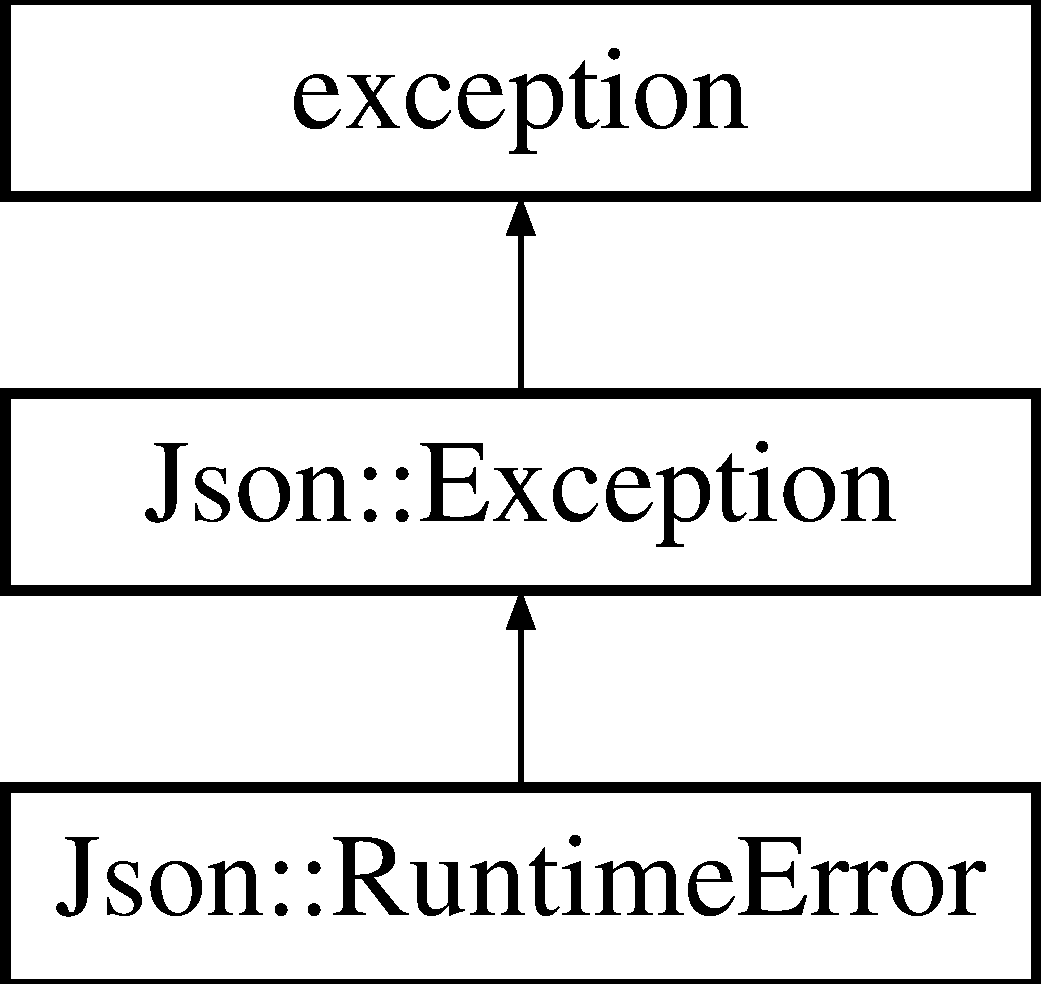
\includegraphics[height=3.307087cm]{class_json_1_1_runtime_error}
\end{center}
\end{figure}
\subsection*{Public Member Functions}
\begin{DoxyCompactItemize}
\item 
{\bfseries Runtime\+Error} (std\+::string const \&msg)\label{class_json_1_1_runtime_error_ae4f102d5c1efb773887efc8c7911e6f8}

\item 
{\bfseries Runtime\+Error} (std\+::string const \&msg)\label{class_json_1_1_runtime_error_ae4f102d5c1efb773887efc8c7911e6f8}

\item 
{\bfseries Runtime\+Error} (std\+::string const \&msg)\label{class_json_1_1_runtime_error_ae4f102d5c1efb773887efc8c7911e6f8}

\item 
{\bfseries Runtime\+Error} (std\+::string const \&msg)\label{class_json_1_1_runtime_error_ae4f102d5c1efb773887efc8c7911e6f8}

\end{DoxyCompactItemize}
\subsection*{Additional Inherited Members}


\subsection{Detailed Description}
Exceptions which the user cannot easily avoid.

E.\+g. out-\/of-\/memory (when we use malloc), stack-\/overflow, malicious input

\begin{DoxyRemark}{Remarks}
derived from \doxyref{Json\+::\+Exception}{p.}{class_json_1_1_exception} 
\end{DoxyRemark}


The documentation for this class was generated from the following files\+:\begin{DoxyCompactItemize}
\item 
api/lib/\+A\+N\+N\+Library/include/json/json.\+h\item 
api/lib/\+A\+N\+N\+Library/src/json/jsoncpp.\+cc\end{DoxyCompactItemize}

\section{Json\+:\+:Static\+String Class Reference}
\label{class_json_1_1_static_string}\index{Json\+::\+Static\+String@{Json\+::\+Static\+String}}


Lightweight wrapper to tag static string.  




{\ttfamily \#include $<$json.\+h$>$}

\subsection*{Public Member Functions}
\begin{DoxyCompactItemize}
\item 
{\bfseries Static\+String} (const char $\ast$czstring)\label{class_json_1_1_static_string_afb6baf1ec078ce76f0b0f9b39d19437f}

\item 
{\bfseries operator const char $\ast$} () const \label{class_json_1_1_static_string_ac2b334d46bbea4c0227e508fc66433e9}

\item 
const char $\ast$ {\bfseries c\+\_\+str} () const \label{class_json_1_1_static_string_ab86fc6a3183adf12fdba4b370acf1754}

\item 
{\bfseries Static\+String} (const char $\ast$czstring)\label{class_json_1_1_static_string_afb6baf1ec078ce76f0b0f9b39d19437f}

\item 
{\bfseries operator const char $\ast$} () const \label{class_json_1_1_static_string_ac2b334d46bbea4c0227e508fc66433e9}

\item 
const char $\ast$ {\bfseries c\+\_\+str} () const \label{class_json_1_1_static_string_ab86fc6a3183adf12fdba4b370acf1754}

\item 
{\bfseries Static\+String} (const char $\ast$czstring)\label{class_json_1_1_static_string_afb6baf1ec078ce76f0b0f9b39d19437f}

\item 
{\bfseries operator const char $\ast$} () const \label{class_json_1_1_static_string_ac2b334d46bbea4c0227e508fc66433e9}

\item 
const char $\ast$ {\bfseries c\+\_\+str} () const \label{class_json_1_1_static_string_ab86fc6a3183adf12fdba4b370acf1754}

\item 
{\bfseries Static\+String} (const char $\ast$czstring)\label{class_json_1_1_static_string_afb6baf1ec078ce76f0b0f9b39d19437f}

\item 
{\bfseries operator const char $\ast$} () const \label{class_json_1_1_static_string_ac2b334d46bbea4c0227e508fc66433e9}

\item 
const char $\ast$ {\bfseries c\+\_\+str} () const \label{class_json_1_1_static_string_ab86fc6a3183adf12fdba4b370acf1754}

\end{DoxyCompactItemize}


\subsection{Detailed Description}
Lightweight wrapper to tag static string. 

\doxyref{Value}{p.}{class_json_1_1_value} constructor and object\+Value member assignement takes advantage of the \doxyref{Static\+String}{p.}{class_json_1_1_static_string} and avoid the cost of string duplication when storing the string or the member name.

Example of usage\+: 
\begin{DoxyCode}
Json::Value aValue( StaticString(\textcolor{stringliteral}{"some text"}) );
Json::Value object;
\textcolor{keyword}{static} \textcolor{keyword}{const} StaticString code(\textcolor{stringliteral}{"code"});
\textcolor{keywordtype}{object}[code] = 1234;
\end{DoxyCode}
 

The documentation for this class was generated from the following file\+:\begin{DoxyCompactItemize}
\item 
/home/robin\+\_\+f/\+Programming/\+Git/\+C\+P\+P/\+Love\+Brains/api/lib/\+A\+N\+N\+Library/include/json/json.\+h\end{DoxyCompactItemize}

\hypertarget{class_json_1_1_stream_writer}{}\section{Json\+:\+:Stream\+Writer Class Reference}
\label{class_json_1_1_stream_writer}\index{Json\+::\+Stream\+Writer@{Json\+::\+Stream\+Writer}}


{\ttfamily \#include $<$json.\+h$>$}

Inheritance diagram for Json\+:\+:Stream\+Writer\+:\begin{figure}[H]
\begin{center}
\leavevmode
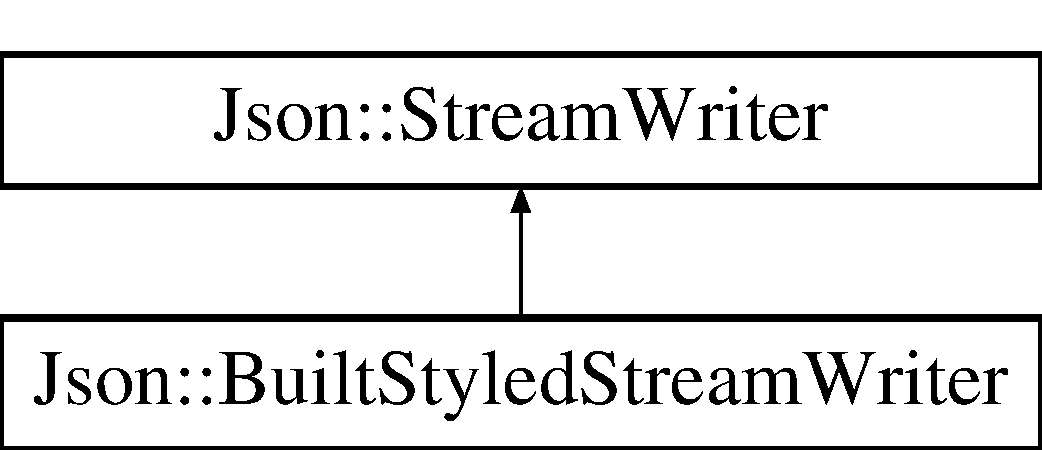
\includegraphics[height=2.000000cm]{class_json_1_1_stream_writer}
\end{center}
\end{figure}
\subsection*{Classes}
\begin{DoxyCompactItemize}
\item 
class \hyperlink{class_json_1_1_stream_writer_1_1_factory}{Factory}
\begin{DoxyCompactList}\small\item\em A simple abstract factory. \end{DoxyCompactList}\end{DoxyCompactItemize}
\subsection*{Public Member Functions}
\begin{DoxyCompactItemize}
\item 
virtual int \hyperlink{class_json_1_1_stream_writer_a237368cf13b41decc015640d25f176ab}{write} (\hyperlink{class_json_1_1_value}{Value} const \&root, std\+::ostream $\ast$sout)=0
\end{DoxyCompactItemize}
\subsection*{Protected Attributes}
\begin{DoxyCompactItemize}
\item 
\hypertarget{class_json_1_1_stream_writer_ac087569ccd2b5a22348cae92ec2a8996}{}std\+::ostream $\ast$ {\bfseries sout\+\_\+}\label{class_json_1_1_stream_writer_ac087569ccd2b5a22348cae92ec2a8996}

\end{DoxyCompactItemize}


\subsection{Detailed Description}
Usage\+: 
\begin{DoxyCode}
\textcolor{keyword}{using namespace }\hyperlink{namespace_json}{Json};
\textcolor{keywordtype}{void} writeToStdout(\hyperlink{class_json_1_1_stream_writer_1_1_factory}{StreamWriter::Factory} \textcolor{keyword}{const}& factory, 
      \hyperlink{class_json_1_1_value}{Value} \textcolor{keyword}{const}& value) \{
  std::unique\_ptr<StreamWriter> \textcolor{keyword}{const} writer(
    factory.\hyperlink{class_json_1_1_stream_writer_1_1_factory_a0fca8d713eb8949ca3ebb35e67f23b1a}{newStreamWriter}());
  writer->write(value, &std::cout);
  std::cout << std::endl;  \textcolor{comment}{// add lf and flush}
\}
\end{DoxyCode}
 

\subsection{Member Function Documentation}
\hypertarget{class_json_1_1_stream_writer_a237368cf13b41decc015640d25f176ab}{}\index{Json\+::\+Stream\+Writer@{Json\+::\+Stream\+Writer}!write@{write}}
\index{write@{write}!Json\+::\+Stream\+Writer@{Json\+::\+Stream\+Writer}}
\subsubsection[{write(\+Value const \&root, std\+::ostream $\ast$sout)=0}]{\setlength{\rightskip}{0pt plus 5cm}virtual int Json\+::\+Stream\+Writer\+::write (
\begin{DoxyParamCaption}
\item[{{\bf Value} const \&}]{root, }
\item[{std\+::ostream $\ast$}]{sout}
\end{DoxyParamCaption}
)\hspace{0.3cm}{\ttfamily [pure virtual]}}\label{class_json_1_1_stream_writer_a237368cf13b41decc015640d25f176ab}
Write \hyperlink{class_json_1_1_value}{Value} into document as configured in sub-\/class. Do not take ownership of sout, but maintain a reference during function. \begin{DoxyPrecond}{Precondition}
sout != N\+U\+L\+L 
\end{DoxyPrecond}
\begin{DoxyReturn}{Returns}
zero on success (For now, we always return zero, so check the stream instead.) 
\end{DoxyReturn}

\begin{DoxyExceptions}{Exceptions}
{\em std\+::exception} & possibly, depending on configuration \\
\hline
\end{DoxyExceptions}


Implemented in \hyperlink{struct_json_1_1_built_styled_stream_writer_ab8810d938c35c8442cbffcd001628cd0}{Json\+::\+Built\+Styled\+Stream\+Writer}.



The documentation for this class was generated from the following files\+:\begin{DoxyCompactItemize}
\item 
/home/robin\+\_\+f/\+Programming/\+Git/\+C\+P\+P/\+Love\+Brains/api/lib/\+A\+N\+N\+Library/include/json/json.\+h\item 
/home/robin\+\_\+f/\+Programming/\+Git/\+C\+P\+P/\+Love\+Brains/api/lib/\+A\+N\+N\+Library/src/json/jsoncpp.\+cc\end{DoxyCompactItemize}

\section{Json\+:\+:Stream\+Writer\+Builder Class Reference}
\label{class_json_1_1_stream_writer_builder}\index{Json\+::\+Stream\+Writer\+Builder@{Json\+::\+Stream\+Writer\+Builder}}


Build a \doxyref{Stream\+Writer}{p.}{class_json_1_1_stream_writer} implementation.  




{\ttfamily \#include $<$json.\+h$>$}

Inheritance diagram for Json\+:\+:Stream\+Writer\+Builder\+:\begin{figure}[H]
\begin{center}
\leavevmode
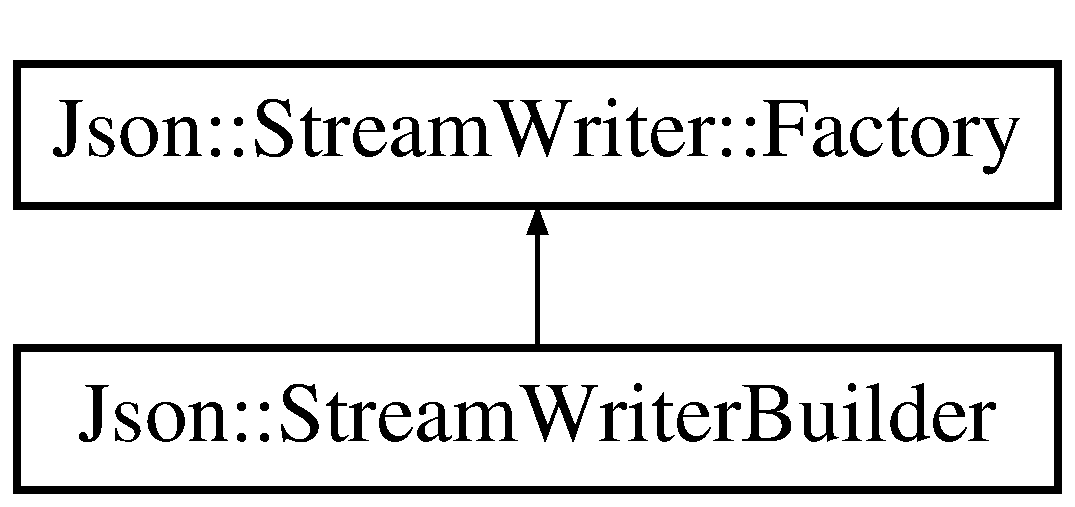
\includegraphics[height=1.590909cm]{class_json_1_1_stream_writer_builder}
\end{center}
\end{figure}
\subsection*{Public Member Functions}
\begin{DoxyCompactItemize}
\item 
virtual {\bf Stream\+Writer} $\ast$ {\bf new\+Stream\+Writer} () const 
\item 
bool {\bf validate} ({\bf Json\+::\+Value} $\ast$invalid) const 
\item 
{\bf Value} \& {\bf operator[$\,$]} (std\+::string key)
\item 
virtual {\bf Stream\+Writer} $\ast$ {\bf new\+Stream\+Writer} () const 
\item 
bool {\bf validate} ({\bf Json\+::\+Value} $\ast$invalid) const 
\item 
{\bf Value} \& {\bf operator[$\,$]} (std\+::string key)
\item 
virtual {\bf Stream\+Writer} $\ast$ {\bf new\+Stream\+Writer} () const 
\item 
bool {\bf validate} ({\bf Json\+::\+Value} $\ast$invalid) const 
\item 
{\bf Value} \& {\bf operator[$\,$]} (std\+::string key)
\item 
virtual {\bf Stream\+Writer} $\ast$ {\bf new\+Stream\+Writer} () const 
\item 
bool {\bf validate} ({\bf Json\+::\+Value} $\ast$invalid) const 
\item 
{\bf Value} \& {\bf operator[$\,$]} (std\+::string key)
\end{DoxyCompactItemize}
\subsection*{Static Public Member Functions}
\begin{DoxyCompactItemize}
\item 
static void {\bf set\+Defaults} ({\bf Json\+::\+Value} $\ast$settings)
\item 
static void {\bf set\+Defaults} ({\bf Json\+::\+Value} $\ast$settings)
\item 
static void {\bf set\+Defaults} ({\bf Json\+::\+Value} $\ast$settings)
\item 
static void {\bf set\+Defaults} ({\bf Json\+::\+Value} $\ast$settings)
\end{DoxyCompactItemize}
\subsection*{Public Attributes}
\begin{DoxyCompactItemize}
\item 
{\bf Json\+::\+Value} {\bf settings\+\_\+}
\end{DoxyCompactItemize}


\subsection{Detailed Description}
Build a \doxyref{Stream\+Writer}{p.}{class_json_1_1_stream_writer} implementation. 

Usage\+: 
\begin{DoxyCode}
\textcolor{keyword}{using namespace }Json;
Value value = ...;
StreamWriterBuilder builder;
builder[\textcolor{stringliteral}{"commentStyle"}] = \textcolor{stringliteral}{"None"};
builder[\textcolor{stringliteral}{"indentation"}] = \textcolor{stringliteral}{"   "};  \textcolor{comment}{// or whatever you like}
std::unique\_ptr<Json::StreamWriter> writer(
    builder.newStreamWriter());
writer->write(value, &std::cout);
std::cout << std::endl;  \textcolor{comment}{// add lf and flush}
\end{DoxyCode}
 

\subsection{Member Function Documentation}
\index{Json\+::\+Stream\+Writer\+Builder@{Json\+::\+Stream\+Writer\+Builder}!new\+Stream\+Writer@{new\+Stream\+Writer}}
\index{new\+Stream\+Writer@{new\+Stream\+Writer}!Json\+::\+Stream\+Writer\+Builder@{Json\+::\+Stream\+Writer\+Builder}}
\subsubsection[{new\+Stream\+Writer() const }]{\setlength{\rightskip}{0pt plus 5cm}{\bf Stream\+Writer} $\ast$ Json\+::\+Stream\+Writer\+Builder\+::new\+Stream\+Writer (
\begin{DoxyParamCaption}
{}
\end{DoxyParamCaption}
) const\hspace{0.3cm}{\ttfamily [virtual]}}\label{class_json_1_1_stream_writer_builder_a96c85792f6680835094917ee93915e4b}

\begin{DoxyExceptions}{Exceptions}
{\em std\+::exception} & if something goes wrong (e.\+g. invalid settings) \\
\hline
\end{DoxyExceptions}


Implements {\bf Json\+::\+Stream\+Writer\+::\+Factory} \doxyref{}{p.}{class_json_1_1_stream_writer_1_1_factory_a0fca8d713eb8949ca3ebb35e67f23b1a}.

\index{Json\+::\+Stream\+Writer\+Builder@{Json\+::\+Stream\+Writer\+Builder}!new\+Stream\+Writer@{new\+Stream\+Writer}}
\index{new\+Stream\+Writer@{new\+Stream\+Writer}!Json\+::\+Stream\+Writer\+Builder@{Json\+::\+Stream\+Writer\+Builder}}
\subsubsection[{new\+Stream\+Writer() const }]{\setlength{\rightskip}{0pt plus 5cm}virtual {\bf Stream\+Writer}$\ast$ Json\+::\+Stream\+Writer\+Builder\+::new\+Stream\+Writer (
\begin{DoxyParamCaption}
{}
\end{DoxyParamCaption}
) const\hspace{0.3cm}{\ttfamily [virtual]}}\label{class_json_1_1_stream_writer_builder_ac7dfbb1cde1c3b9fa0781c1b8885bdff}

\begin{DoxyExceptions}{Exceptions}
{\em std\+::exception} & if something goes wrong (e.\+g. invalid settings) \\
\hline
\end{DoxyExceptions}


Implements {\bf Json\+::\+Stream\+Writer\+::\+Factory} \doxyref{}{p.}{class_json_1_1_stream_writer_1_1_factory_a0fca8d713eb8949ca3ebb35e67f23b1a}.

\index{Json\+::\+Stream\+Writer\+Builder@{Json\+::\+Stream\+Writer\+Builder}!new\+Stream\+Writer@{new\+Stream\+Writer}}
\index{new\+Stream\+Writer@{new\+Stream\+Writer}!Json\+::\+Stream\+Writer\+Builder@{Json\+::\+Stream\+Writer\+Builder}}
\subsubsection[{new\+Stream\+Writer() const }]{\setlength{\rightskip}{0pt plus 5cm}virtual {\bf Stream\+Writer}$\ast$ Json\+::\+Stream\+Writer\+Builder\+::new\+Stream\+Writer (
\begin{DoxyParamCaption}
{}
\end{DoxyParamCaption}
) const\hspace{0.3cm}{\ttfamily [virtual]}}\label{class_json_1_1_stream_writer_builder_ac7dfbb1cde1c3b9fa0781c1b8885bdff}

\begin{DoxyExceptions}{Exceptions}
{\em std\+::exception} & if something goes wrong (e.\+g. invalid settings) \\
\hline
\end{DoxyExceptions}


Implements {\bf Json\+::\+Stream\+Writer\+::\+Factory} \doxyref{}{p.}{class_json_1_1_stream_writer_1_1_factory_a0fca8d713eb8949ca3ebb35e67f23b1a}.

\index{Json\+::\+Stream\+Writer\+Builder@{Json\+::\+Stream\+Writer\+Builder}!new\+Stream\+Writer@{new\+Stream\+Writer}}
\index{new\+Stream\+Writer@{new\+Stream\+Writer}!Json\+::\+Stream\+Writer\+Builder@{Json\+::\+Stream\+Writer\+Builder}}
\subsubsection[{new\+Stream\+Writer() const }]{\setlength{\rightskip}{0pt plus 5cm}virtual {\bf Stream\+Writer}$\ast$ Json\+::\+Stream\+Writer\+Builder\+::new\+Stream\+Writer (
\begin{DoxyParamCaption}
{}
\end{DoxyParamCaption}
) const\hspace{0.3cm}{\ttfamily [virtual]}}\label{class_json_1_1_stream_writer_builder_ac7dfbb1cde1c3b9fa0781c1b8885bdff}

\begin{DoxyExceptions}{Exceptions}
{\em std\+::exception} & if something goes wrong (e.\+g. invalid settings) \\
\hline
\end{DoxyExceptions}


Implements {\bf Json\+::\+Stream\+Writer\+::\+Factory} \doxyref{}{p.}{class_json_1_1_stream_writer_1_1_factory_a0fca8d713eb8949ca3ebb35e67f23b1a}.

\index{Json\+::\+Stream\+Writer\+Builder@{Json\+::\+Stream\+Writer\+Builder}!operator[$\,$]@{operator[]}}
\index{operator[$\,$]@{operator[]}!Json\+::\+Stream\+Writer\+Builder@{Json\+::\+Stream\+Writer\+Builder}}
\subsubsection[{operator[](std\+::string key)}]{\setlength{\rightskip}{0pt plus 5cm}{\bf Value}\& Json\+::\+Stream\+Writer\+Builder\+::operator[$\,$] (
\begin{DoxyParamCaption}
\item[{std\+::string}]{key}
\end{DoxyParamCaption}
)}\label{class_json_1_1_stream_writer_builder_a4484fbb004d912da7e45d65deb0ee05b}
A simple way to update a specific setting. \index{Json\+::\+Stream\+Writer\+Builder@{Json\+::\+Stream\+Writer\+Builder}!operator[$\,$]@{operator[]}}
\index{operator[$\,$]@{operator[]}!Json\+::\+Stream\+Writer\+Builder@{Json\+::\+Stream\+Writer\+Builder}}
\subsubsection[{operator[](std\+::string key)}]{\setlength{\rightskip}{0pt plus 5cm}{\bf Value}\& Json\+::\+Stream\+Writer\+Builder\+::operator[$\,$] (
\begin{DoxyParamCaption}
\item[{std\+::string}]{key}
\end{DoxyParamCaption}
)}\label{class_json_1_1_stream_writer_builder_a4484fbb004d912da7e45d65deb0ee05b}
A simple way to update a specific setting. \index{Json\+::\+Stream\+Writer\+Builder@{Json\+::\+Stream\+Writer\+Builder}!operator[$\,$]@{operator[]}}
\index{operator[$\,$]@{operator[]}!Json\+::\+Stream\+Writer\+Builder@{Json\+::\+Stream\+Writer\+Builder}}
\subsubsection[{operator[](std\+::string key)}]{\setlength{\rightskip}{0pt plus 5cm}{\bf Value} \& Json\+::\+Stream\+Writer\+Builder\+::operator[$\,$] (
\begin{DoxyParamCaption}
\item[{std\+::string}]{key}
\end{DoxyParamCaption}
)}\label{class_json_1_1_stream_writer_builder_aa010a8a04a92343179f64a5dbb5df340}
A simple way to update a specific setting. \index{Json\+::\+Stream\+Writer\+Builder@{Json\+::\+Stream\+Writer\+Builder}!operator[$\,$]@{operator[]}}
\index{operator[$\,$]@{operator[]}!Json\+::\+Stream\+Writer\+Builder@{Json\+::\+Stream\+Writer\+Builder}}
\subsubsection[{operator[](std\+::string key)}]{\setlength{\rightskip}{0pt plus 5cm}{\bf Value}\& Json\+::\+Stream\+Writer\+Builder\+::operator[$\,$] (
\begin{DoxyParamCaption}
\item[{std\+::string}]{key}
\end{DoxyParamCaption}
)}\label{class_json_1_1_stream_writer_builder_a4484fbb004d912da7e45d65deb0ee05b}
A simple way to update a specific setting. \index{Json\+::\+Stream\+Writer\+Builder@{Json\+::\+Stream\+Writer\+Builder}!set\+Defaults@{set\+Defaults}}
\index{set\+Defaults@{set\+Defaults}!Json\+::\+Stream\+Writer\+Builder@{Json\+::\+Stream\+Writer\+Builder}}
\subsubsection[{set\+Defaults(\+Json\+::\+Value $\ast$settings)}]{\setlength{\rightskip}{0pt plus 5cm}static void Json\+::\+Stream\+Writer\+Builder\+::set\+Defaults (
\begin{DoxyParamCaption}
\item[{{\bf Json\+::\+Value} $\ast$}]{settings}
\end{DoxyParamCaption}
)\hspace{0.3cm}{\ttfamily [static]}}\label{class_json_1_1_stream_writer_builder_a886224c308545b54ed242b436cdc90d3}
Called by ctor, but you can use this to reset settings\+\_\+. \begin{DoxyPrecond}{Precondition}
\textquotesingle{}settings\textquotesingle{} != N\+U\+L\+L (but Json\+::null is fine) 
\end{DoxyPrecond}
\begin{DoxyRemark}{Remarks}
Defaults\+: 
\begin{DoxyCodeInclude}
\end{DoxyCodeInclude}

\end{DoxyRemark}
\index{Json\+::\+Stream\+Writer\+Builder@{Json\+::\+Stream\+Writer\+Builder}!set\+Defaults@{set\+Defaults}}
\index{set\+Defaults@{set\+Defaults}!Json\+::\+Stream\+Writer\+Builder@{Json\+::\+Stream\+Writer\+Builder}}
\subsubsection[{set\+Defaults(\+Json\+::\+Value $\ast$settings)}]{\setlength{\rightskip}{0pt plus 5cm}static void Json\+::\+Stream\+Writer\+Builder\+::set\+Defaults (
\begin{DoxyParamCaption}
\item[{{\bf Json\+::\+Value} $\ast$}]{settings}
\end{DoxyParamCaption}
)\hspace{0.3cm}{\ttfamily [static]}}\label{class_json_1_1_stream_writer_builder_a886224c308545b54ed242b436cdc90d3}
Called by ctor, but you can use this to reset settings\+\_\+. \begin{DoxyPrecond}{Precondition}
\textquotesingle{}settings\textquotesingle{} != N\+U\+L\+L (but Json\+::null is fine) 
\end{DoxyPrecond}
\begin{DoxyRemark}{Remarks}
Defaults\+: 
\begin{DoxyCodeInclude}
\end{DoxyCodeInclude}

\end{DoxyRemark}
\index{Json\+::\+Stream\+Writer\+Builder@{Json\+::\+Stream\+Writer\+Builder}!set\+Defaults@{set\+Defaults}}
\index{set\+Defaults@{set\+Defaults}!Json\+::\+Stream\+Writer\+Builder@{Json\+::\+Stream\+Writer\+Builder}}
\subsubsection[{set\+Defaults(\+Json\+::\+Value $\ast$settings)}]{\setlength{\rightskip}{0pt plus 5cm}void Json\+::\+Stream\+Writer\+Builder\+::set\+Defaults (
\begin{DoxyParamCaption}
\item[{{\bf Json\+::\+Value} $\ast$}]{settings}
\end{DoxyParamCaption}
)\hspace{0.3cm}{\ttfamily [static]}}\label{class_json_1_1_stream_writer_builder_a53bf106b141e28637b01ad0ecd2acbf6}
Called by ctor, but you can use this to reset settings\+\_\+. \begin{DoxyPrecond}{Precondition}
\textquotesingle{}settings\textquotesingle{} != N\+U\+L\+L (but Json\+::null is fine) 
\end{DoxyPrecond}
\begin{DoxyRemark}{Remarks}
Defaults\+: 
\begin{DoxyCodeInclude}
\end{DoxyCodeInclude}

\end{DoxyRemark}
[Stream\+Writer\+Builder\+Defaults]

[Stream\+Writer\+Builder\+Defaults]

[Stream\+Writer\+Builder\+Defaults]

[Stream\+Writer\+Builder\+Defaults]

[Stream\+Writer\+Builder\+Defaults]

[Stream\+Writer\+Builder\+Defaults] \index{Json\+::\+Stream\+Writer\+Builder@{Json\+::\+Stream\+Writer\+Builder}!set\+Defaults@{set\+Defaults}}
\index{set\+Defaults@{set\+Defaults}!Json\+::\+Stream\+Writer\+Builder@{Json\+::\+Stream\+Writer\+Builder}}
\subsubsection[{set\+Defaults(\+Json\+::\+Value $\ast$settings)}]{\setlength{\rightskip}{0pt plus 5cm}static void Json\+::\+Stream\+Writer\+Builder\+::set\+Defaults (
\begin{DoxyParamCaption}
\item[{{\bf Json\+::\+Value} $\ast$}]{settings}
\end{DoxyParamCaption}
)\hspace{0.3cm}{\ttfamily [static]}}\label{class_json_1_1_stream_writer_builder_a886224c308545b54ed242b436cdc90d3}
Called by ctor, but you can use this to reset settings\+\_\+. \begin{DoxyPrecond}{Precondition}
\textquotesingle{}settings\textquotesingle{} != N\+U\+L\+L (but Json\+::null is fine) 
\end{DoxyPrecond}
\begin{DoxyRemark}{Remarks}
Defaults\+: 
\begin{DoxyCodeInclude}
\end{DoxyCodeInclude}

\end{DoxyRemark}
\index{Json\+::\+Stream\+Writer\+Builder@{Json\+::\+Stream\+Writer\+Builder}!validate@{validate}}
\index{validate@{validate}!Json\+::\+Stream\+Writer\+Builder@{Json\+::\+Stream\+Writer\+Builder}}
\subsubsection[{validate(\+Json\+::\+Value $\ast$invalid) const }]{\setlength{\rightskip}{0pt plus 5cm}bool Json\+::\+Stream\+Writer\+Builder\+::validate (
\begin{DoxyParamCaption}
\item[{{\bf Json\+::\+Value} $\ast$}]{invalid}
\end{DoxyParamCaption}
) const}\label{class_json_1_1_stream_writer_builder_aa1dfed085a3d369e953e4a3c34da009e}
\begin{DoxyReturn}{Returns}
true if \textquotesingle{}settings\textquotesingle{} are legal and consistent; otherwise, indicate bad settings via \textquotesingle{}invalid\textquotesingle{}. 
\end{DoxyReturn}
\index{Json\+::\+Stream\+Writer\+Builder@{Json\+::\+Stream\+Writer\+Builder}!validate@{validate}}
\index{validate@{validate}!Json\+::\+Stream\+Writer\+Builder@{Json\+::\+Stream\+Writer\+Builder}}
\subsubsection[{validate(\+Json\+::\+Value $\ast$invalid) const }]{\setlength{\rightskip}{0pt plus 5cm}bool Json\+::\+Stream\+Writer\+Builder\+::validate (
\begin{DoxyParamCaption}
\item[{{\bf Json\+::\+Value} $\ast$}]{invalid}
\end{DoxyParamCaption}
) const}\label{class_json_1_1_stream_writer_builder_aa1dfed085a3d369e953e4a3c34da009e}
\begin{DoxyReturn}{Returns}
true if \textquotesingle{}settings\textquotesingle{} are legal and consistent; otherwise, indicate bad settings via \textquotesingle{}invalid\textquotesingle{}. 
\end{DoxyReturn}
\index{Json\+::\+Stream\+Writer\+Builder@{Json\+::\+Stream\+Writer\+Builder}!validate@{validate}}
\index{validate@{validate}!Json\+::\+Stream\+Writer\+Builder@{Json\+::\+Stream\+Writer\+Builder}}
\subsubsection[{validate(\+Json\+::\+Value $\ast$invalid) const }]{\setlength{\rightskip}{0pt plus 5cm}bool Json\+::\+Stream\+Writer\+Builder\+::validate (
\begin{DoxyParamCaption}
\item[{{\bf Json\+::\+Value} $\ast$}]{invalid}
\end{DoxyParamCaption}
) const}\label{class_json_1_1_stream_writer_builder_aa1dfed085a3d369e953e4a3c34da009e}
\begin{DoxyReturn}{Returns}
true if \textquotesingle{}settings\textquotesingle{} are legal and consistent; otherwise, indicate bad settings via \textquotesingle{}invalid\textquotesingle{}. 
\end{DoxyReturn}
\index{Json\+::\+Stream\+Writer\+Builder@{Json\+::\+Stream\+Writer\+Builder}!validate@{validate}}
\index{validate@{validate}!Json\+::\+Stream\+Writer\+Builder@{Json\+::\+Stream\+Writer\+Builder}}
\subsubsection[{validate(\+Json\+::\+Value $\ast$invalid) const }]{\setlength{\rightskip}{0pt plus 5cm}bool Json\+::\+Stream\+Writer\+Builder\+::validate (
\begin{DoxyParamCaption}
\item[{{\bf Json\+::\+Value} $\ast$}]{invalid}
\end{DoxyParamCaption}
) const}\label{class_json_1_1_stream_writer_builder_aa1dfed085a3d369e953e4a3c34da009e}
\begin{DoxyReturn}{Returns}
true if \textquotesingle{}settings\textquotesingle{} are legal and consistent; otherwise, indicate bad settings via \textquotesingle{}invalid\textquotesingle{}. 
\end{DoxyReturn}


\subsection{Member Data Documentation}
\index{Json\+::\+Stream\+Writer\+Builder@{Json\+::\+Stream\+Writer\+Builder}!settings\+\_\+@{settings\+\_\+}}
\index{settings\+\_\+@{settings\+\_\+}!Json\+::\+Stream\+Writer\+Builder@{Json\+::\+Stream\+Writer\+Builder}}
\subsubsection[{settings\+\_\+}]{\setlength{\rightskip}{0pt plus 5cm}{\bf Json\+::\+Value} Json\+::\+Stream\+Writer\+Builder\+::settings\+\_\+}\label{class_json_1_1_stream_writer_builder_a79bdf2e639a52f4e758c0b95bd1d3423}
Configuration of this builder. Available settings (case-\/sensitive)\+:
\begin{DoxyItemize}
\item \char`\"{}comment\+Style\char`\"{}\+: \char`\"{}\+None\char`\"{} or \char`\"{}\+All\char`\"{}
\item \char`\"{}indentation\char`\"{}\+: \char`\"{}$<$anything$>$\char`\"{}
\item \char`\"{}enable\+Y\+A\+M\+L\+Compatibility\char`\"{}\+: false or true
\begin{DoxyItemize}
\item slightly change the whitespace around colons
\end{DoxyItemize}
\item \char`\"{}drop\+Null\+Placeholders\char`\"{}\+: false or true
\begin{DoxyItemize}
\item Drop the \char`\"{}null\char`\"{} string from the writer\textquotesingle{}s output for null\+Values. Strictly speaking, this is not valid J\+S\+O\+N. But when the output is being fed to a browser\textquotesingle{}s Javascript, it makes for smaller output and the browser can handle the output just fine.
\end{DoxyItemize}
\end{DoxyItemize}

You can examine \textquotesingle{}settings\+\_\+` yourself to see the defaults. You can also write and read them just like any J\+S\+O\+N \doxyref{Value}{p.}{class_json_1_1_value}. \begin{DoxySeeAlso}{See also}
\doxyref{set\+Defaults()}{p.}{class_json_1_1_stream_writer_builder_a53bf106b141e28637b01ad0ecd2acbf6} 
\end{DoxySeeAlso}


The documentation for this class was generated from the following files\+:\begin{DoxyCompactItemize}
\item 
api/lib/\+A\+N\+N\+Library/include/json/json.\+h\item 
api/lib/\+A\+N\+N\+Library/src/json/jsoncpp.\+cc\end{DoxyCompactItemize}

\section{Json\+:\+:Our\+Reader\+:\+:Structured\+Error Struct Reference}
\label{struct_json_1_1_our_reader_1_1_structured_error}\index{Json\+::\+Our\+Reader\+::\+Structured\+Error@{Json\+::\+Our\+Reader\+::\+Structured\+Error}}
\subsection*{Public Attributes}
\begin{DoxyCompactItemize}
\item 
size\+\_\+t {\bfseries offset\+\_\+start}\label{struct_json_1_1_our_reader_1_1_structured_error_a4eec161c2a6b4c89b6eb3d8d83834443}

\item 
size\+\_\+t {\bfseries offset\+\_\+limit}\label{struct_json_1_1_our_reader_1_1_structured_error_a6bab2650e5230fc15427b309de79fdbe}

\item 
std\+::string {\bfseries message}\label{struct_json_1_1_our_reader_1_1_structured_error_adc8a757b6452cc6ab14fb90b933b3414}

\end{DoxyCompactItemize}


The documentation for this struct was generated from the following file\+:\begin{DoxyCompactItemize}
\item 
/home/robin\+\_\+f/\+Programming/\+Git/\+C\+P\+P/\+Love\+Brains/api/lib/\+A\+N\+N\+Library/src/json/jsoncpp.\+cc\end{DoxyCompactItemize}

\section{Json\+:\+:Reader\+:\+:Structured\+Error Struct Reference}
\label{struct_json_1_1_reader_1_1_structured_error}\index{Json\+::\+Reader\+::\+Structured\+Error@{Json\+::\+Reader\+::\+Structured\+Error}}


An error tagged with where in the J\+S\+O\+N text it was encountered.  




{\ttfamily \#include $<$json.\+h$>$}

\subsection*{Public Attributes}
\begin{DoxyCompactItemize}
\item 
size\+\_\+t {\bfseries offset\+\_\+start}\label{struct_json_1_1_reader_1_1_structured_error_a160dae4eb3464a2209b743c755baf65f}

\item 
size\+\_\+t {\bfseries offset\+\_\+limit}\label{struct_json_1_1_reader_1_1_structured_error_a80747dae744bcc80a9bc81c94fd42e13}

\item 
std\+::string {\bfseries message}\label{struct_json_1_1_reader_1_1_structured_error_ab8755e5201b78c6ae077338f8819e6e6}

\end{DoxyCompactItemize}


\subsection{Detailed Description}
An error tagged with where in the J\+S\+O\+N text it was encountered. 

The offsets give the [start, limit) range of bytes within the text. Note that this is bytes, not codepoints. 

The documentation for this struct was generated from the following file\+:\begin{DoxyCompactItemize}
\item 
api/lib/\+A\+N\+N\+Library/include/json/json.\+h\end{DoxyCompactItemize}

\section{Json\+:\+:Styled\+Stream\+Writer Class Reference}
\label{class_json_1_1_styled_stream_writer}\index{Json\+::\+Styled\+Stream\+Writer@{Json\+::\+Styled\+Stream\+Writer}}


Writes a \doxyref{Value}{p.}{class_json_1_1_value} in {\tt J\+S\+O\+N} format in a human friendly way, to a stream rather than to a string.  




{\ttfamily \#include $<$json.\+h$>$}

\subsection*{Public Member Functions}
\begin{DoxyCompactItemize}
\item 
{\bfseries Styled\+Stream\+Writer} (std\+::string indentation=\char`\"{}\textbackslash{}t\char`\"{})\label{class_json_1_1_styled_stream_writer_ae87567a08de865b6dc84d7218a3001df}

\item 
void {\bf write} (std\+::ostream \&out, const {\bf Value} \&root)
\begin{DoxyCompactList}\small\item\em Serialize a \doxyref{Value}{p.}{class_json_1_1_value} in {\tt J\+S\+O\+N} format. \end{DoxyCompactList}\item 
{\bfseries Styled\+Stream\+Writer} (std\+::string indentation=\char`\"{}\textbackslash{}t\char`\"{})\label{class_json_1_1_styled_stream_writer_ae87567a08de865b6dc84d7218a3001df}

\item 
void {\bf write} (std\+::ostream \&out, const {\bf Value} \&root)
\begin{DoxyCompactList}\small\item\em Serialize a \doxyref{Value}{p.}{class_json_1_1_value} in {\tt J\+S\+O\+N} format. \end{DoxyCompactList}\end{DoxyCompactItemize}


\subsection{Detailed Description}
Writes a \doxyref{Value}{p.}{class_json_1_1_value} in {\tt J\+S\+O\+N} format in a human friendly way, to a stream rather than to a string. 

The rules for line break and indent are as follow\+:
\begin{DoxyItemize}
\item Object value\+:
\begin{DoxyItemize}
\item if empty then print \{\} without indent and line break
\item if not empty the print \textquotesingle{}\{\textquotesingle{}, line break \& indent, print one value per line and then unindent and line break and print \textquotesingle{}\}\textquotesingle{}.
\end{DoxyItemize}
\item Array value\+:
\begin{DoxyItemize}
\item if empty then print [] without indent and line break
\item if the array contains no object value, empty array or some other value types, and all the values fit on one lines, then print the array on a single line.
\item otherwise, it the values do not fit on one line, or the array contains object or non empty array, then print one value per line.
\end{DoxyItemize}
\end{DoxyItemize}

If the \doxyref{Value}{p.}{class_json_1_1_value} have comments then they are outputed according to their \doxyref{Comment\+Placement}{p.}{namespace_json_a4fc417c23905b2ae9e2c47d197a45351}.


\begin{DoxyParams}{Parameters}
{\em indentation} & Each level will be indented by this amount extra. \\
\hline
\end{DoxyParams}
\begin{DoxySeeAlso}{See also}
\doxyref{Reader}{p.}{class_json_1_1_reader}, \doxyref{Value}{p.}{class_json_1_1_value}, \doxyref{Value\+::set\+Comment()}{p.}{class_json_1_1_value_a29f3a30f7e5d3af6f38d57999bf5b480} 
\end{DoxySeeAlso}
\begin{DoxyRefDesc}{Deprecated}
\item[{\bf Deprecated}]Use \doxyref{Stream\+Writer\+Builder}{p.}{class_json_1_1_stream_writer_builder}. \end{DoxyRefDesc}


The rules for line break and indent are as follow\+:
\begin{DoxyItemize}
\item Object value\+:
\begin{DoxyItemize}
\item if empty then print \{\} without indent and line break
\item if not empty the print \textquotesingle{}\{\textquotesingle{}, line break \& indent, print one value per line and then unindent and line break and print \textquotesingle{}\}\textquotesingle{}.
\end{DoxyItemize}
\item Array value\+:
\begin{DoxyItemize}
\item if empty then print [] without indent and line break
\item if the array contains no object value, empty array or some other value types, and all the values fit on one lines, then print the array on a single line.
\item otherwise, it the values do not fit on one line, or the array contains object or non empty array, then print one value per line.
\end{DoxyItemize}
\end{DoxyItemize}

If the \doxyref{Value}{p.}{class_json_1_1_value} have comments then they are outputed according to their \doxyref{Comment\+Placement}{p.}{namespace_json_a4fc417c23905b2ae9e2c47d197a45351}.


\begin{DoxyParams}{Parameters}
{\em indentation} & Each level will be indented by this amount extra. \\
\hline
\end{DoxyParams}
\begin{DoxySeeAlso}{See also}
\doxyref{Reader}{p.}{class_json_1_1_reader}, \doxyref{Value}{p.}{class_json_1_1_value}, \doxyref{Value\+::set\+Comment()}{p.}{class_json_1_1_value_a29f3a30f7e5d3af6f38d57999bf5b480} 
\end{DoxySeeAlso}
\begin{DoxyRefDesc}{Deprecated}
\item[{\bf Deprecated}]Use \doxyref{Stream\+Writer\+Builder}{p.}{class_json_1_1_stream_writer_builder}. \end{DoxyRefDesc}


\subsection{Member Function Documentation}
\index{Json\+::\+Styled\+Stream\+Writer@{Json\+::\+Styled\+Stream\+Writer}!write@{write}}
\index{write@{write}!Json\+::\+Styled\+Stream\+Writer@{Json\+::\+Styled\+Stream\+Writer}}
\subsubsection[{write(std\+::ostream \&out, const Value \&root)}]{\setlength{\rightskip}{0pt plus 5cm}void Json\+::\+Styled\+Stream\+Writer\+::write (
\begin{DoxyParamCaption}
\item[{std\+::ostream \&}]{out, }
\item[{const {\bf Value} \&}]{root}
\end{DoxyParamCaption}
)}\label{class_json_1_1_styled_stream_writer_a07807741c6c43ecd35885a87234d0805}


Serialize a \doxyref{Value}{p.}{class_json_1_1_value} in {\tt J\+S\+O\+N} format. 


\begin{DoxyParams}{Parameters}
{\em out} & Stream to write to. (Can be ostringstream, e.\+g.) \\
\hline
{\em root} & \doxyref{Value}{p.}{class_json_1_1_value} to serialize. \\
\hline
\end{DoxyParams}
\begin{DoxyNote}{Note}
There is no point in deriving from \doxyref{Writer}{p.}{class_json_1_1_writer}, since \doxyref{write()}{p.}{class_json_1_1_styled_stream_writer_a07807741c6c43ecd35885a87234d0805} should not return a value. 
\end{DoxyNote}
\index{Json\+::\+Styled\+Stream\+Writer@{Json\+::\+Styled\+Stream\+Writer}!write@{write}}
\index{write@{write}!Json\+::\+Styled\+Stream\+Writer@{Json\+::\+Styled\+Stream\+Writer}}
\subsubsection[{write(std\+::ostream \&out, const Value \&root)}]{\setlength{\rightskip}{0pt plus 5cm}void Json\+::\+Styled\+Stream\+Writer\+::write (
\begin{DoxyParamCaption}
\item[{std\+::ostream \&}]{out, }
\item[{const {\bf Value} \&}]{root}
\end{DoxyParamCaption}
)}\label{class_json_1_1_styled_stream_writer_a07807741c6c43ecd35885a87234d0805}


Serialize a \doxyref{Value}{p.}{class_json_1_1_value} in {\tt J\+S\+O\+N} format. 


\begin{DoxyParams}{Parameters}
{\em out} & Stream to write to. (Can be ostringstream, e.\+g.) \\
\hline
{\em root} & \doxyref{Value}{p.}{class_json_1_1_value} to serialize. \\
\hline
\end{DoxyParams}
\begin{DoxyNote}{Note}
There is no point in deriving from \doxyref{Writer}{p.}{class_json_1_1_writer}, since \doxyref{write()}{p.}{class_json_1_1_styled_stream_writer_a07807741c6c43ecd35885a87234d0805} should not return a value. 
\end{DoxyNote}


The documentation for this class was generated from the following files\+:\begin{DoxyCompactItemize}
\item 
/home/robin\+\_\+f/\+Programming/\+Git/\+C\+P\+P/\+Love\+Brains/include/json/json.\+h\item 
/home/robin\+\_\+f/\+Programming/\+Git/\+C\+P\+P/\+Love\+Brains/lib/\+G\+A\+N\+N\+Engine/src/json/jsoncpp.\+cc\end{DoxyCompactItemize}

\hypertarget{class_json_1_1_styled_writer}{}\section{Json\+:\+:Styled\+Writer Class Reference}
\label{class_json_1_1_styled_writer}\index{Json\+::\+Styled\+Writer@{Json\+::\+Styled\+Writer}}


Writes a \hyperlink{class_json_1_1_value}{Value} in \href{http://www.json.org}{\tt J\+S\+O\+N} format in a human friendly way.  




{\ttfamily \#include $<$json.\+h$>$}

Inheritance diagram for Json\+:\+:Styled\+Writer\+:\begin{figure}[H]
\begin{center}
\leavevmode
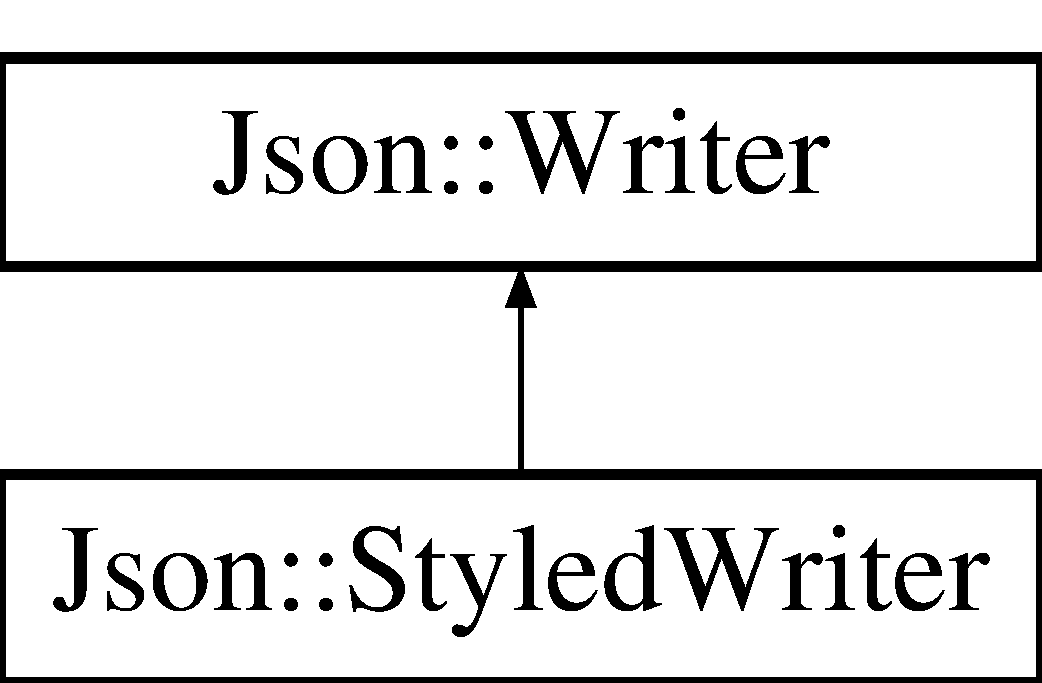
\includegraphics[height=2.000000cm]{class_json_1_1_styled_writer}
\end{center}
\end{figure}
\subsection*{Public Member Functions}
\begin{DoxyCompactItemize}
\item 
virtual std\+::string \hyperlink{class_json_1_1_styled_writer_a56f0fd80f60272b3f3c85690aae66e7d}{write} (const \hyperlink{class_json_1_1_value}{Value} \&root)
\begin{DoxyCompactList}\small\item\em Serialize a \hyperlink{class_json_1_1_value}{Value} in \href{http://www.json.org}{\tt J\+S\+O\+N} format. \end{DoxyCompactList}\end{DoxyCompactItemize}


\subsection{Detailed Description}
Writes a \hyperlink{class_json_1_1_value}{Value} in \href{http://www.json.org}{\tt J\+S\+O\+N} format in a human friendly way. 

The rules for line break and indent are as follow\+:
\begin{DoxyItemize}
\item Object value\+:
\begin{DoxyItemize}
\item if empty then print \{\} without indent and line break
\item if not empty the print \textquotesingle{}\{\textquotesingle{}, line break \& indent, print one value per line and then unindent and line break and print \textquotesingle{}\}\textquotesingle{}.
\end{DoxyItemize}
\item Array value\+:
\begin{DoxyItemize}
\item if empty then print \mbox{[}\mbox{]} without indent and line break
\item if the array contains no object value, empty array or some other value types, and all the values fit on one lines, then print the array on a single line.
\item otherwise, it the values do not fit on one line, or the array contains object or non empty array, then print one value per line.
\end{DoxyItemize}
\end{DoxyItemize}

If the \hyperlink{class_json_1_1_value}{Value} have comments then they are outputed according to their \hyperlink{namespace_json_a4fc417c23905b2ae9e2c47d197a45351}{Comment\+Placement}.

\begin{DoxySeeAlso}{See also}
\hyperlink{class_json_1_1_reader}{Reader}, \hyperlink{class_json_1_1_value}{Value}, \hyperlink{class_json_1_1_value_a29f3a30f7e5d3af6f38d57999bf5b480}{Value\+::set\+Comment()} 
\end{DoxySeeAlso}
\begin{DoxyRefDesc}{Deprecated}
\item[\hyperlink{deprecated__deprecated000009}{Deprecated}]Use \hyperlink{class_json_1_1_stream_writer_builder}{Stream\+Writer\+Builder}. \end{DoxyRefDesc}


\subsection{Member Function Documentation}
\hypertarget{class_json_1_1_styled_writer_a56f0fd80f60272b3f3c85690aae66e7d}{}\index{Json\+::\+Styled\+Writer@{Json\+::\+Styled\+Writer}!write@{write}}
\index{write@{write}!Json\+::\+Styled\+Writer@{Json\+::\+Styled\+Writer}}
\subsubsection[{write(const Value \&root)}]{\setlength{\rightskip}{0pt plus 5cm}std\+::string Json\+::\+Styled\+Writer\+::write (
\begin{DoxyParamCaption}
\item[{const {\bf Value} \&}]{root}
\end{DoxyParamCaption}
)\hspace{0.3cm}{\ttfamily [virtual]}}\label{class_json_1_1_styled_writer_a56f0fd80f60272b3f3c85690aae66e7d}


Serialize a \hyperlink{class_json_1_1_value}{Value} in \href{http://www.json.org}{\tt J\+S\+O\+N} format. 


\begin{DoxyParams}{Parameters}
{\em root} & \hyperlink{class_json_1_1_value}{Value} to serialize. \\
\hline
\end{DoxyParams}
\begin{DoxyReturn}{Returns}
String containing the J\+S\+O\+N document that represents the root value. 
\end{DoxyReturn}


Implements \hyperlink{class_json_1_1_writer}{Json\+::\+Writer}.



The documentation for this class was generated from the following files\+:\begin{DoxyCompactItemize}
\item 
/home/robin\+\_\+f/\+Programming/\+Git/\+C\+P\+P/\+Love\+Brains/api/lib/\+A\+N\+N\+Library/include/json/json.\+h\item 
/home/robin\+\_\+f/\+Programming/\+Git/\+C\+P\+P/\+Love\+Brains/api/lib/\+A\+N\+N\+Library/src/json/jsoncpp.\+cc\end{DoxyCompactItemize}

\hypertarget{class_json_1_1_value}{}\section{Json\+:\+:Value Class Reference}
\label{class_json_1_1_value}\index{Json\+::\+Value@{Json\+::\+Value}}


Represents a \href{http://www.json.org}{\tt J\+S\+O\+N} value.  




{\ttfamily \#include $<$json.\+h$>$}

\subsection*{Public Types}
\begin{DoxyCompactItemize}
\item 
\hypertarget{class_json_1_1_value_ac61bab5a465848b57610379cc07995c3}{}typedef std\+::vector$<$ std\+::string $>$ {\bfseries Members}\label{class_json_1_1_value_ac61bab5a465848b57610379cc07995c3}

\item 
\hypertarget{class_json_1_1_value_a341cdf2e01f8b3c5b7317aa2f0768c53}{}typedef \hyperlink{class_json_1_1_value_iterator}{Value\+Iterator} {\bfseries iterator}\label{class_json_1_1_value_a341cdf2e01f8b3c5b7317aa2f0768c53}

\item 
\hypertarget{class_json_1_1_value_af92282ca92b58b320debd486afb7696a}{}typedef \hyperlink{class_json_1_1_value_const_iterator}{Value\+Const\+Iterator} {\bfseries const\+\_\+iterator}\label{class_json_1_1_value_af92282ca92b58b320debd486afb7696a}

\item 
\hypertarget{class_json_1_1_value_a0933d59b45793ae4aade1757c322a98d}{}typedef Json\+::\+U\+Int {\bfseries U\+Int}\label{class_json_1_1_value_a0933d59b45793ae4aade1757c322a98d}

\item 
\hypertarget{class_json_1_1_value_abdf7a7ff73eb130ffcab28504ffdb405}{}typedef Json\+::\+Int {\bfseries Int}\label{class_json_1_1_value_abdf7a7ff73eb130ffcab28504ffdb405}

\item 
\hypertarget{class_json_1_1_value_a8b62564be8c087c6d18de180ff4e13e3}{}typedef Json\+::\+U\+Int64 {\bfseries U\+Int64}\label{class_json_1_1_value_a8b62564be8c087c6d18de180ff4e13e3}

\item 
\hypertarget{class_json_1_1_value_a1b86af9f85f0f1baa972c3319fa22695}{}typedef Json\+::\+Int64 {\bfseries Int64}\label{class_json_1_1_value_a1b86af9f85f0f1baa972c3319fa22695}

\item 
\hypertarget{class_json_1_1_value_a1cbb82642ed05109b9833e49f042ece7}{}typedef Json\+::\+Largest\+Int {\bfseries Largest\+Int}\label{class_json_1_1_value_a1cbb82642ed05109b9833e49f042ece7}

\item 
\hypertarget{class_json_1_1_value_a6682a3684d635e03fc06ba229fa24eec}{}typedef Json\+::\+Largest\+U\+Int {\bfseries Largest\+U\+Int}\label{class_json_1_1_value_a6682a3684d635e03fc06ba229fa24eec}

\item 
\hypertarget{class_json_1_1_value_a184a91566cccca7b819240f0d5561c7d}{}typedef Json\+::\+Array\+Index {\bfseries Array\+Index}\label{class_json_1_1_value_a184a91566cccca7b819240f0d5561c7d}

\item 
\hypertarget{class_json_1_1_value_a08b6c80c3af7071d908dabf044de5388}{}typedef std\+::map$<$ C\+Z\+String, \hyperlink{class_json_1_1_value}{Value} $>$ {\bfseries Object\+Values}\label{class_json_1_1_value_a08b6c80c3af7071d908dabf044de5388}

\end{DoxyCompactItemize}
\subsection*{Public Member Functions}
\begin{DoxyCompactItemize}
\item 
\hyperlink{class_json_1_1_value_ada6ba1369448fb0240bccc36efaa46f7}{Value} (\hyperlink{namespace_json_a7d654b75c16a57007925868e38212b4e}{Value\+Type} type=\hyperlink{namespace_json_a7d654b75c16a57007925868e38212b4ea7d9899633b4409bd3fc107e6737f8391}{null\+Value})
\begin{DoxyCompactList}\small\item\em Create a default \hyperlink{class_json_1_1_value}{Value} of the given type. \end{DoxyCompactList}\item 
\hypertarget{class_json_1_1_value_a4744ae571fcf34f4b16a2257b3b3b585}{}{\bfseries Value} (Int value)\label{class_json_1_1_value_a4744ae571fcf34f4b16a2257b3b3b585}

\item 
\hypertarget{class_json_1_1_value_ae67a857b01286e3499a87e95be848d20}{}{\bfseries Value} (U\+Int value)\label{class_json_1_1_value_ae67a857b01286e3499a87e95be848d20}

\item 
\hypertarget{class_json_1_1_value_ab1cdc3d9a4d4cc03fa01439d43ceb1b5}{}{\bfseries Value} (Int64 value)\label{class_json_1_1_value_ab1cdc3d9a4d4cc03fa01439d43ceb1b5}

\item 
\hypertarget{class_json_1_1_value_a8adda58d5ae17bf7ca6a53bab4a7b69c}{}{\bfseries Value} (U\+Int64 value)\label{class_json_1_1_value_a8adda58d5ae17bf7ca6a53bab4a7b69c}

\item 
\hypertarget{class_json_1_1_value_a32228cc84d83200cca8441451997996c}{}{\bfseries Value} (double value)\label{class_json_1_1_value_a32228cc84d83200cca8441451997996c}

\item 
\hypertarget{class_json_1_1_value_ad87b849356816aca75995dd07302e49d}{}\hyperlink{class_json_1_1_value_ad87b849356816aca75995dd07302e49d}{Value} (const char $\ast$value)\label{class_json_1_1_value_ad87b849356816aca75995dd07302e49d}

\begin{DoxyCompactList}\small\item\em Copy til first 0. (N\+U\+L\+L causes to seg-\/fault.) \end{DoxyCompactList}\item 
\hypertarget{class_json_1_1_value_a39fa09d1902efbd4350e1236db920571}{}\hyperlink{class_json_1_1_value_a39fa09d1902efbd4350e1236db920571}{Value} (const char $\ast$begin, const char $\ast$end)\label{class_json_1_1_value_a39fa09d1902efbd4350e1236db920571}

\begin{DoxyCompactList}\small\item\em Copy all, incl zeroes. \end{DoxyCompactList}\item 
\hyperlink{class_json_1_1_value_a081830e95f88a37054da7e46c65b0766}{Value} (const \hyperlink{class_json_1_1_static_string}{Static\+String} \&value)
\begin{DoxyCompactList}\small\item\em Constructs a value from a static string. \end{DoxyCompactList}\item 
\hypertarget{class_json_1_1_value_aa4501dd4edf3ce3d5145fc656f088b21}{}\hyperlink{class_json_1_1_value_aa4501dd4edf3ce3d5145fc656f088b21}{Value} (const std\+::string \&value)\label{class_json_1_1_value_aa4501dd4edf3ce3d5145fc656f088b21}

\begin{DoxyCompactList}\small\item\em Copy data() til \hyperlink{class_json_1_1_value_a4ca8ee6c48a34ca6c2f131956bab5e05}{size()}. Embedded zeroes too. \end{DoxyCompactList}\item 
\hypertarget{class_json_1_1_value_a350a31ea4a30d384994b0bc010b17495}{}{\bfseries Value} (bool value)\label{class_json_1_1_value_a350a31ea4a30d384994b0bc010b17495}

\item 
\hypertarget{class_json_1_1_value_a436dfd3670f95fd665f680eba5cebcf0}{}\hyperlink{class_json_1_1_value_a436dfd3670f95fd665f680eba5cebcf0}{Value} (const \hyperlink{class_json_1_1_value}{Value} \&other)\label{class_json_1_1_value_a436dfd3670f95fd665f680eba5cebcf0}

\begin{DoxyCompactList}\small\item\em Deep copy. \end{DoxyCompactList}\item 
\hyperlink{class_json_1_1_value}{Value} \& \hyperlink{class_json_1_1_value_a795acb28772da4c5d85ae8f4af36c69f}{operator=} (\hyperlink{class_json_1_1_value}{Value} other)
\item 
\hypertarget{class_json_1_1_value_aab841120d78e296e1bc06a373345e822}{}void \hyperlink{class_json_1_1_value_aab841120d78e296e1bc06a373345e822}{swap} (\hyperlink{class_json_1_1_value}{Value} \&other)\label{class_json_1_1_value_aab841120d78e296e1bc06a373345e822}

\begin{DoxyCompactList}\small\item\em Swap everything. \end{DoxyCompactList}\item 
\hypertarget{class_json_1_1_value_a5263476047f20e2fc6de470e4de34fe5}{}void \hyperlink{class_json_1_1_value_a5263476047f20e2fc6de470e4de34fe5}{swap\+Payload} (\hyperlink{class_json_1_1_value}{Value} \&other)\label{class_json_1_1_value_a5263476047f20e2fc6de470e4de34fe5}

\begin{DoxyCompactList}\small\item\em Swap values but leave comments and source offsets in place. \end{DoxyCompactList}\item 
\hypertarget{class_json_1_1_value_a695ef31fad36b4712918b3ff80158479}{}\hyperlink{namespace_json_a7d654b75c16a57007925868e38212b4e}{Value\+Type} {\bfseries type} () const \label{class_json_1_1_value_a695ef31fad36b4712918b3ff80158479}

\item 
\hypertarget{class_json_1_1_value_af0ad8aa027575c3277296458f3fb7b0a}{}bool \hyperlink{class_json_1_1_value_af0ad8aa027575c3277296458f3fb7b0a}{operator$<$} (const \hyperlink{class_json_1_1_value}{Value} \&other) const \label{class_json_1_1_value_af0ad8aa027575c3277296458f3fb7b0a}

\begin{DoxyCompactList}\small\item\em Compare payload only, not comments etc. \end{DoxyCompactList}\item 
\hypertarget{class_json_1_1_value_afb99dd3628fe44244b32007f9b4f369a}{}bool {\bfseries operator$<$=} (const \hyperlink{class_json_1_1_value}{Value} \&other) const \label{class_json_1_1_value_afb99dd3628fe44244b32007f9b4f369a}

\item 
\hypertarget{class_json_1_1_value_acc13fc47d55abd6e2327b090b83d2911}{}bool {\bfseries operator$>$=} (const \hyperlink{class_json_1_1_value}{Value} \&other) const \label{class_json_1_1_value_acc13fc47d55abd6e2327b090b83d2911}

\item 
\hypertarget{class_json_1_1_value_a3124a26067bdfde9571bc89527fc6931}{}bool {\bfseries operator$>$} (const \hyperlink{class_json_1_1_value}{Value} \&other) const \label{class_json_1_1_value_a3124a26067bdfde9571bc89527fc6931}

\item 
\hypertarget{class_json_1_1_value_a14363dda23a6ae2def9afd1590ae85d3}{}bool {\bfseries operator==} (const \hyperlink{class_json_1_1_value}{Value} \&other) const \label{class_json_1_1_value_a14363dda23a6ae2def9afd1590ae85d3}

\item 
\hypertarget{class_json_1_1_value_ad0f12d2a4ab74bbef08a05504b2cb81d}{}bool {\bfseries operator!=} (const \hyperlink{class_json_1_1_value}{Value} \&other) const \label{class_json_1_1_value_ad0f12d2a4ab74bbef08a05504b2cb81d}

\item 
\hypertarget{class_json_1_1_value_a899214ed2253d3f4f061b922b0e622b5}{}int {\bfseries compare} (const \hyperlink{class_json_1_1_value}{Value} \&other) const \label{class_json_1_1_value_a899214ed2253d3f4f061b922b0e622b5}

\item 
\hypertarget{class_json_1_1_value_a5b7da48b163bcec63b1424f1608b7da6}{}const char $\ast$ \hyperlink{class_json_1_1_value_a5b7da48b163bcec63b1424f1608b7da6}{as\+C\+String} () const \label{class_json_1_1_value_a5b7da48b163bcec63b1424f1608b7da6}

\begin{DoxyCompactList}\small\item\em Embedded zeroes could cause you trouble! \end{DoxyCompactList}\item 
\hypertarget{class_json_1_1_value_a03ee3d5df576640c93ba683f140828bd}{}std\+::string \hyperlink{class_json_1_1_value_a03ee3d5df576640c93ba683f140828bd}{as\+String} () const \label{class_json_1_1_value_a03ee3d5df576640c93ba683f140828bd}

\begin{DoxyCompactList}\small\item\em Embedded zeroes are possible. \end{DoxyCompactList}\item 
bool \hyperlink{class_json_1_1_value_a1e0263113ae247a632afac43ebc4149f}{get\+String} (char const $\ast$$\ast$begin, char const $\ast$$\ast$end) const 
\item 
\hypertarget{class_json_1_1_value_ac786e35b860b1d700cb3d3e56dd6a235}{}Int {\bfseries as\+Int} () const \label{class_json_1_1_value_ac786e35b860b1d700cb3d3e56dd6a235}

\item 
\hypertarget{class_json_1_1_value_a2019d1bd296b89356c1b0da5970c918c}{}U\+Int {\bfseries as\+U\+Int} () const \label{class_json_1_1_value_a2019d1bd296b89356c1b0da5970c918c}

\item 
\hypertarget{class_json_1_1_value_a4451cee7524534458894f4e2cc045aa3}{}Int64 {\bfseries as\+Int64} () const \label{class_json_1_1_value_a4451cee7524534458894f4e2cc045aa3}

\item 
\hypertarget{class_json_1_1_value_a4aa617bc0625ae0f208fa54b7c6326ad}{}U\+Int64 {\bfseries as\+U\+Int64} () const \label{class_json_1_1_value_a4aa617bc0625ae0f208fa54b7c6326ad}

\item 
\hypertarget{class_json_1_1_value_a3786bb100c5cf9a98eb6d13784968956}{}Largest\+Int {\bfseries as\+Largest\+Int} () const \label{class_json_1_1_value_a3786bb100c5cf9a98eb6d13784968956}

\item 
\hypertarget{class_json_1_1_value_a692b88345a745b2f89ca5d94b52e94d4}{}Largest\+U\+Int {\bfseries as\+Largest\+U\+Int} () const \label{class_json_1_1_value_a692b88345a745b2f89ca5d94b52e94d4}

\item 
\hypertarget{class_json_1_1_value_ac2128d7080499daf8c5b1c71da243f63}{}float {\bfseries as\+Float} () const \label{class_json_1_1_value_ac2128d7080499daf8c5b1c71da243f63}

\item 
\hypertarget{class_json_1_1_value_a33434ed1c0217a34d04c95fa5342fd37}{}double {\bfseries as\+Double} () const \label{class_json_1_1_value_a33434ed1c0217a34d04c95fa5342fd37}

\item 
\hypertarget{class_json_1_1_value_a7402c797285c020566c3db5f8ae4e940}{}bool {\bfseries as\+Bool} () const \label{class_json_1_1_value_a7402c797285c020566c3db5f8ae4e940}

\item 
\hypertarget{class_json_1_1_value_aeb9ad8b1bb91bdd72203dc884b3f4362}{}bool {\bfseries is\+Null} () const \label{class_json_1_1_value_aeb9ad8b1bb91bdd72203dc884b3f4362}

\item 
\hypertarget{class_json_1_1_value_a3c3716cc7a0216cb1b654bb8f61c8d13}{}bool {\bfseries is\+Bool} () const \label{class_json_1_1_value_a3c3716cc7a0216cb1b654bb8f61c8d13}

\item 
\hypertarget{class_json_1_1_value_ab0df4746d6787d2ce1db1a156c118f14}{}bool {\bfseries is\+Int} () const \label{class_json_1_1_value_ab0df4746d6787d2ce1db1a156c118f14}

\item 
\hypertarget{class_json_1_1_value_aba89690e5fd72d0f7121a30013470423}{}bool {\bfseries is\+Int64} () const \label{class_json_1_1_value_aba89690e5fd72d0f7121a30013470423}

\item 
\hypertarget{class_json_1_1_value_ae814ca1796fe2d43ac09898b70213989}{}bool {\bfseries is\+U\+Int} () const \label{class_json_1_1_value_ae814ca1796fe2d43ac09898b70213989}

\item 
\hypertarget{class_json_1_1_value_aa35efece2a6cba4d988d7d5b54db2fb8}{}bool {\bfseries is\+U\+Int64} () const \label{class_json_1_1_value_aa35efece2a6cba4d988d7d5b54db2fb8}

\item 
\hypertarget{class_json_1_1_value_aec4f74ef7b776b1d9c8a10fc3bb4add5}{}bool {\bfseries is\+Integral} () const \label{class_json_1_1_value_aec4f74ef7b776b1d9c8a10fc3bb4add5}

\item 
\hypertarget{class_json_1_1_value_a0ea567fa51fc808851698bef59b43626}{}bool {\bfseries is\+Double} () const \label{class_json_1_1_value_a0ea567fa51fc808851698bef59b43626}

\item 
\hypertarget{class_json_1_1_value_a8ce848900e2e8fa23a41fcc2c1409fab}{}bool {\bfseries is\+Numeric} () const \label{class_json_1_1_value_a8ce848900e2e8fa23a41fcc2c1409fab}

\item 
\hypertarget{class_json_1_1_value_a06c01d7c1e8151a5844b595ab00f46c7}{}bool {\bfseries is\+String} () const \label{class_json_1_1_value_a06c01d7c1e8151a5844b595ab00f46c7}

\item 
\hypertarget{class_json_1_1_value_ac8c898f93543e55b67418f94bced20af}{}bool {\bfseries is\+Array} () const \label{class_json_1_1_value_ac8c898f93543e55b67418f94bced20af}

\item 
\hypertarget{class_json_1_1_value_a80cffaa0402b80317c0437216bbb6d92}{}bool {\bfseries is\+Object} () const \label{class_json_1_1_value_a80cffaa0402b80317c0437216bbb6d92}

\item 
\hypertarget{class_json_1_1_value_a7ec153803631a27abf58cba2bb1af70c}{}bool {\bfseries is\+Convertible\+To} (\hyperlink{namespace_json_a7d654b75c16a57007925868e38212b4e}{Value\+Type} other) const \label{class_json_1_1_value_a7ec153803631a27abf58cba2bb1af70c}

\item 
\hypertarget{class_json_1_1_value_a4ca8ee6c48a34ca6c2f131956bab5e05}{}Array\+Index \hyperlink{class_json_1_1_value_a4ca8ee6c48a34ca6c2f131956bab5e05}{size} () const \label{class_json_1_1_value_a4ca8ee6c48a34ca6c2f131956bab5e05}

\begin{DoxyCompactList}\small\item\em Number of values in array or object. \end{DoxyCompactList}\item 
\hypertarget{class_json_1_1_value_a99c42d3ff8495dad1e91b43e66553c36}{}bool \hyperlink{class_json_1_1_value_a99c42d3ff8495dad1e91b43e66553c36}{empty} () const \label{class_json_1_1_value_a99c42d3ff8495dad1e91b43e66553c36}

\begin{DoxyCompactList}\small\item\em Return true if empty array, empty object, or null; otherwise, false. \end{DoxyCompactList}\item 
\hypertarget{class_json_1_1_value_a021ab0d15a807fbe051446c9c545ab61}{}bool \hyperlink{class_json_1_1_value_a021ab0d15a807fbe051446c9c545ab61}{operator!} () const \label{class_json_1_1_value_a021ab0d15a807fbe051446c9c545ab61}

\begin{DoxyCompactList}\small\item\em Return is\+Null() \end{DoxyCompactList}\item 
void \hyperlink{class_json_1_1_value_a501a4d67e6c875255c2ecc03ccd2019b}{clear} ()
\item 
void \hyperlink{class_json_1_1_value_aa284353271ada427dbfa04a42f2be407}{resize} (Array\+Index \hyperlink{class_json_1_1_value_a4ca8ee6c48a34ca6c2f131956bab5e05}{size})
\item 
\hyperlink{class_json_1_1_value}{Value} \& \hyperlink{class_json_1_1_value_a7d99f5dba388cdaa152ce6ef933d64ef}{operator\mbox{[}$\,$\mbox{]}} (Array\+Index index)
\item 
\hyperlink{class_json_1_1_value}{Value} \& \hyperlink{class_json_1_1_value_ac9182982c361e0ab621134d406e5f250}{operator\mbox{[}$\,$\mbox{]}} (int index)
\item 
const \hyperlink{class_json_1_1_value}{Value} \& \hyperlink{class_json_1_1_value_af151919e8947c430e34bed2b0b128601}{operator\mbox{[}$\,$\mbox{]}} (Array\+Index index) const 
\item 
const \hyperlink{class_json_1_1_value}{Value} \& \hyperlink{class_json_1_1_value_af9e02b38f4e63e491c300c20b275bdd7}{operator\mbox{[}$\,$\mbox{]}} (int index) const 
\item 
\hyperlink{class_json_1_1_value}{Value} \hyperlink{class_json_1_1_value_a28282c9b76fa031eba7a1843c47c16fe}{get} (Array\+Index index, const \hyperlink{class_json_1_1_value}{Value} \&default\+Value) const 
\item 
\hypertarget{class_json_1_1_value_aaa82ebb4b730ea1567d310874f47d147}{}bool \hyperlink{class_json_1_1_value_aaa82ebb4b730ea1567d310874f47d147}{is\+Valid\+Index} (Array\+Index index) const \label{class_json_1_1_value_aaa82ebb4b730ea1567d310874f47d147}

\begin{DoxyCompactList}\small\item\em Return true if index $<$ \hyperlink{class_json_1_1_value_a4ca8ee6c48a34ca6c2f131956bab5e05}{size()}. \end{DoxyCompactList}\item 
\hyperlink{class_json_1_1_value}{Value} \& \hyperlink{class_json_1_1_value_a7e49ac977e4bcf59745a09d426669f75}{append} (const \hyperlink{class_json_1_1_value}{Value} \&value)
\begin{DoxyCompactList}\small\item\em Append value to array at the end. \end{DoxyCompactList}\item 
\hyperlink{class_json_1_1_value}{Value} \& \hyperlink{class_json_1_1_value_acb912f4ec40a25ea6eb387730885f3d9}{operator\mbox{[}$\,$\mbox{]}} (const char $\ast$key)
\item 
const \hyperlink{class_json_1_1_value}{Value} \& \hyperlink{class_json_1_1_value_ae5f73ffc7a039bca81b7ca771bc5db55}{operator\mbox{[}$\,$\mbox{]}} (const char $\ast$key) const 
\item 
\hyperlink{class_json_1_1_value}{Value} \& \hyperlink{class_json_1_1_value_ae511c7d46bf457412fb55c9471af9f50}{operator\mbox{[}$\,$\mbox{]}} (const std\+::string \&key)
\item 
const \hyperlink{class_json_1_1_value}{Value} \& \hyperlink{class_json_1_1_value_a3c53bfd2381d5a61036d7dc0b023d697}{operator\mbox{[}$\,$\mbox{]}} (const std\+::string \&key) const 
\item 
\hyperlink{class_json_1_1_value}{Value} \& \hyperlink{class_json_1_1_value_ac3763d7d315ca65dc188e273722f7955}{operator\mbox{[}$\,$\mbox{]}} (const \hyperlink{class_json_1_1_static_string}{Static\+String} \&key)
\begin{DoxyCompactList}\small\item\em Access an object value by name, create a null member if it does not exist. \end{DoxyCompactList}\item 
\hyperlink{class_json_1_1_value}{Value} \hyperlink{class_json_1_1_value_ab76b3323cde14c7db20676d07b260ce7}{get} (const char $\ast$key, const \hyperlink{class_json_1_1_value}{Value} \&default\+Value) const 
\item 
\hyperlink{class_json_1_1_value}{Value} \hyperlink{class_json_1_1_value_abcb2289c005bc0befdedaa94f662f63f}{get} (const char $\ast$begin, const char $\ast$end, const \hyperlink{class_json_1_1_value}{Value} \&default\+Value) const 
\item 
\hyperlink{class_json_1_1_value}{Value} \hyperlink{class_json_1_1_value_a54a34264356e01ee9c21a75ccfc809e9}{get} (const std\+::string \&key, const \hyperlink{class_json_1_1_value}{Value} \&default\+Value) const 
\item 
\hyperlink{class_json_1_1_value}{Value} const $\ast$ \hyperlink{class_json_1_1_value_a184bf49ec5da7ec31af089cf6f458f99}{find} (char const $\ast$begin, char const $\ast$end) const 
\item 
\hyperlink{class_json_1_1_value}{Value} const $\ast$ \hyperlink{class_json_1_1_value_afeb7ff596a0929d90c5f2f3cffb413ed}{demand} (char const $\ast$begin, char const $\ast$end)
\item 
\hyperlink{class_json_1_1_value}{Value} \hyperlink{class_json_1_1_value_aa52f7873b95d29627d6e83ba96f69aaa}{remove\+Member} (const char $\ast$key)
\begin{DoxyCompactList}\small\item\em Remove and return the named member. \end{DoxyCompactList}\item 
\hyperlink{class_json_1_1_value}{Value} \hyperlink{class_json_1_1_value_ae1f95f7ca3906e6bcc2a7be93210ecba}{remove\+Member} (const std\+::string \&key)
\item 
bool \hyperlink{class_json_1_1_value_a708e599489adf30d65bf85a8ee16e6fb}{remove\+Member} (const char $\ast$key, \hyperlink{class_json_1_1_value}{Value} $\ast$removed)
\item 
bool \hyperlink{class_json_1_1_value_a3749dae413a73eac05b7f8dc6deeb6a2}{remove\+Member} (std\+::string const \&key, \hyperlink{class_json_1_1_value}{Value} $\ast$removed)
\begin{DoxyCompactList}\small\item\em Remove the named map member. \end{DoxyCompactList}\item 
\hypertarget{class_json_1_1_value_a49c91af727d6b4eb0af02a81bb2def87}{}bool \hyperlink{class_json_1_1_value_a49c91af727d6b4eb0af02a81bb2def87}{remove\+Member} (const char $\ast$begin, const char $\ast$end, \hyperlink{class_json_1_1_value}{Value} $\ast$removed)\label{class_json_1_1_value_a49c91af727d6b4eb0af02a81bb2def87}

\begin{DoxyCompactList}\small\item\em Same as \hyperlink{class_json_1_1_value_a3749dae413a73eac05b7f8dc6deeb6a2}{remove\+Member(std\+::string const\& key, Value$\ast$ removed)} \end{DoxyCompactList}\item 
bool \hyperlink{class_json_1_1_value_ae9e67e08a85a2f3be3396ec0f4c47f65}{remove\+Index} (Array\+Index i, \hyperlink{class_json_1_1_value}{Value} $\ast$removed)
\begin{DoxyCompactList}\small\item\em Remove the indexed array element. \end{DoxyCompactList}\item 
bool \hyperlink{class_json_1_1_value_a196defba501d70ea2b6793afb04108e3}{is\+Member} (const char $\ast$key) const 
\item 
bool \hyperlink{class_json_1_1_value_af728b5738aaa133f3aad2e39dc4f415e}{is\+Member} (const std\+::string \&key) const 
\item 
\hypertarget{class_json_1_1_value_a077604b87a79d75543a1b5438eb9d8ab}{}bool \hyperlink{class_json_1_1_value_a077604b87a79d75543a1b5438eb9d8ab}{is\+Member} (const char $\ast$begin, const char $\ast$end) const \label{class_json_1_1_value_a077604b87a79d75543a1b5438eb9d8ab}

\begin{DoxyCompactList}\small\item\em Same as is\+Member(std\+::string const\& key)const. \end{DoxyCompactList}\item 
Members \hyperlink{class_json_1_1_value_a30fa08af88f2d0a038b22ba9f4e88b2a}{get\+Member\+Names} () const 
\begin{DoxyCompactList}\small\item\em Return a list of the member names. \end{DoxyCompactList}\item 
void \hyperlink{class_json_1_1_value_a29f3a30f7e5d3af6f38d57999bf5b480}{set\+Comment} (const char $\ast$comment, \hyperlink{namespace_json_a4fc417c23905b2ae9e2c47d197a45351}{Comment\+Placement} placement)
\item 
\hypertarget{class_json_1_1_value_a2900152a2887b410a9ddabe278b9d492}{}void \hyperlink{class_json_1_1_value_a2900152a2887b410a9ddabe278b9d492}{set\+Comment} (const char $\ast$comment, size\+\_\+t len, \hyperlink{namespace_json_a4fc417c23905b2ae9e2c47d197a45351}{Comment\+Placement} placement)\label{class_json_1_1_value_a2900152a2887b410a9ddabe278b9d492}

\begin{DoxyCompactList}\small\item\em Comments must be //... or /$\ast$ ... $\ast$/. \end{DoxyCompactList}\item 
\hypertarget{class_json_1_1_value_a6d68a2e7d4e1e317cd9e812e12181689}{}void \hyperlink{class_json_1_1_value_a6d68a2e7d4e1e317cd9e812e12181689}{set\+Comment} (const std\+::string \&comment, \hyperlink{namespace_json_a4fc417c23905b2ae9e2c47d197a45351}{Comment\+Placement} placement)\label{class_json_1_1_value_a6d68a2e7d4e1e317cd9e812e12181689}

\begin{DoxyCompactList}\small\item\em Comments must be //... or /$\ast$ ... $\ast$/. \end{DoxyCompactList}\item 
\hypertarget{class_json_1_1_value_a06567a00363cab9601be7e31336db03a}{}bool {\bfseries has\+Comment} (\hyperlink{namespace_json_a4fc417c23905b2ae9e2c47d197a45351}{Comment\+Placement} placement) const \label{class_json_1_1_value_a06567a00363cab9601be7e31336db03a}

\item 
\hypertarget{class_json_1_1_value_aa1e105b5d7f55d6e42f4fb2f3674116f}{}std\+::string \hyperlink{class_json_1_1_value_aa1e105b5d7f55d6e42f4fb2f3674116f}{get\+Comment} (\hyperlink{namespace_json_a4fc417c23905b2ae9e2c47d197a45351}{Comment\+Placement} placement) const \label{class_json_1_1_value_aa1e105b5d7f55d6e42f4fb2f3674116f}

\begin{DoxyCompactList}\small\item\em Include delimiters and embedded newlines. \end{DoxyCompactList}\item 
\hypertarget{class_json_1_1_value_a05357cf78959b790337fae4e5580ee4f}{}std\+::string {\bfseries to\+Styled\+String} () const \label{class_json_1_1_value_a05357cf78959b790337fae4e5580ee4f}

\item 
\hypertarget{class_json_1_1_value_ac12df0d6980600c5bac908ed0f64856e}{}\hyperlink{class_json_1_1_value_const_iterator}{const\+\_\+iterator} {\bfseries begin} () const \label{class_json_1_1_value_ac12df0d6980600c5bac908ed0f64856e}

\item 
\hypertarget{class_json_1_1_value_a596da1926b2f2a4056bff2edb713eb0b}{}\hyperlink{class_json_1_1_value_const_iterator}{const\+\_\+iterator} {\bfseries end} () const \label{class_json_1_1_value_a596da1926b2f2a4056bff2edb713eb0b}

\item 
\hypertarget{class_json_1_1_value_a2d45bb2e68e8f22fe356d7d955ebd3c9}{}\hyperlink{class_json_1_1_value_iterator}{iterator} {\bfseries begin} ()\label{class_json_1_1_value_a2d45bb2e68e8f22fe356d7d955ebd3c9}

\item 
\hypertarget{class_json_1_1_value_a2f961eff73f7f79cd29260b6cbd42558}{}\hyperlink{class_json_1_1_value_iterator}{iterator} {\bfseries end} ()\label{class_json_1_1_value_a2f961eff73f7f79cd29260b6cbd42558}

\item 
\hypertarget{class_json_1_1_value_a6d741407c3d784360c200f181b0d6d64}{}void {\bfseries set\+Offset\+Start} (size\+\_\+t start)\label{class_json_1_1_value_a6d741407c3d784360c200f181b0d6d64}

\item 
\hypertarget{class_json_1_1_value_ac6d858b5fd4d5fe6ca84f697def8c5ea}{}void {\bfseries set\+Offset\+Limit} (size\+\_\+t limit)\label{class_json_1_1_value_ac6d858b5fd4d5fe6ca84f697def8c5ea}

\item 
\hypertarget{class_json_1_1_value_a10142eda11ae0b1caecbcc9f436854d1}{}size\+\_\+t {\bfseries get\+Offset\+Start} () const \label{class_json_1_1_value_a10142eda11ae0b1caecbcc9f436854d1}

\item 
\hypertarget{class_json_1_1_value_acd7114469bc39368e9d93c29b54d8c8f}{}size\+\_\+t {\bfseries get\+Offset\+Limit} () const \label{class_json_1_1_value_acd7114469bc39368e9d93c29b54d8c8f}

\end{DoxyCompactItemize}
\subsection*{Static Public Attributes}
\begin{DoxyCompactItemize}
\item 
\hypertarget{class_json_1_1_value_a6d6e9ea6807e46d5b7ded66d3032f607}{}static const \hyperlink{class_json_1_1_value}{Value} \& \hyperlink{class_json_1_1_value_a6d6e9ea6807e46d5b7ded66d3032f607}{null} = reinterpret\+\_\+cast$<$const \hyperlink{class_json_1_1_value}{Value}\&$>$(k\+Null\+Ref)\label{class_json_1_1_value_a6d6e9ea6807e46d5b7ded66d3032f607}

\begin{DoxyCompactList}\small\item\em We regret this reference to a global instance; prefer the simpler \hyperlink{class_json_1_1_value_ada6ba1369448fb0240bccc36efaa46f7}{Value()}. \end{DoxyCompactList}\item 
static const \hyperlink{class_json_1_1_value}{Value} \& \hyperlink{class_json_1_1_value_aaa4ffd4e53967170c3e8c9abf682b5cd}{null\+Ref} = \hyperlink{class_json_1_1_value_a6d6e9ea6807e46d5b7ded66d3032f607}{null}
\item 
\hypertarget{class_json_1_1_value_af91df130daa50dd43d2cd89e6ee67706}{}static const Largest\+Int \hyperlink{class_json_1_1_value_af91df130daa50dd43d2cd89e6ee67706}{min\+Largest\+Int} = Largest\+Int($\sim$(Largest\+U\+Int(-\/1) / 2))\label{class_json_1_1_value_af91df130daa50dd43d2cd89e6ee67706}

\begin{DoxyCompactList}\small\item\em Minimum signed integer value that can be stored in a \hyperlink{class_json_1_1_value}{Json\+::\+Value}. \end{DoxyCompactList}\item 
\hypertarget{class_json_1_1_value_a8b4977696f13296fa8755c7953fafb2f}{}static const Largest\+Int \hyperlink{class_json_1_1_value_a8b4977696f13296fa8755c7953fafb2f}{max\+Largest\+Int} = Largest\+Int(Largest\+U\+Int(-\/1) / 2)\label{class_json_1_1_value_a8b4977696f13296fa8755c7953fafb2f}

\begin{DoxyCompactList}\small\item\em Maximum signed integer value that can be stored in a \hyperlink{class_json_1_1_value}{Json\+::\+Value}. \end{DoxyCompactList}\item 
\hypertarget{class_json_1_1_value_a8ddb32d9d55fa5323ae5135639dc2e31}{}static const Largest\+U\+Int \hyperlink{class_json_1_1_value_a8ddb32d9d55fa5323ae5135639dc2e31}{max\+Largest\+U\+Int} = Largest\+U\+Int(-\/1)\label{class_json_1_1_value_a8ddb32d9d55fa5323ae5135639dc2e31}

\begin{DoxyCompactList}\small\item\em Maximum unsigned integer value that can be stored in a \hyperlink{class_json_1_1_value}{Json\+::\+Value}. \end{DoxyCompactList}\item 
\hypertarget{class_json_1_1_value_a7df8a39e2502b8c92a6a41e3d752d2c8}{}static const Int \hyperlink{class_json_1_1_value_a7df8a39e2502b8c92a6a41e3d752d2c8}{min\+Int} = Int($\sim$(U\+Int(-\/1) / 2))\label{class_json_1_1_value_a7df8a39e2502b8c92a6a41e3d752d2c8}

\begin{DoxyCompactList}\small\item\em Minimum signed int value that can be stored in a \hyperlink{class_json_1_1_value}{Json\+::\+Value}. \end{DoxyCompactList}\item 
\hypertarget{class_json_1_1_value_a978c799a8af3114ef7dab6fd0a310a1b}{}static const Int \hyperlink{class_json_1_1_value_a978c799a8af3114ef7dab6fd0a310a1b}{max\+Int} = Int(U\+Int(-\/1) / 2)\label{class_json_1_1_value_a978c799a8af3114ef7dab6fd0a310a1b}

\begin{DoxyCompactList}\small\item\em Maximum signed int value that can be stored in a \hyperlink{class_json_1_1_value}{Json\+::\+Value}. \end{DoxyCompactList}\item 
\hypertarget{class_json_1_1_value_ac79e63ee68d3aa914bfd6988be669b87}{}static const U\+Int \hyperlink{class_json_1_1_value_ac79e63ee68d3aa914bfd6988be669b87}{max\+U\+Int} = U\+Int(-\/1)\label{class_json_1_1_value_ac79e63ee68d3aa914bfd6988be669b87}

\begin{DoxyCompactList}\small\item\em Maximum unsigned int value that can be stored in a \hyperlink{class_json_1_1_value}{Json\+::\+Value}. \end{DoxyCompactList}\item 
\hypertarget{class_json_1_1_value_a815ef899bc312c93bc426511acfe31a7}{}static const Int64 \hyperlink{class_json_1_1_value_a815ef899bc312c93bc426511acfe31a7}{min\+Int64}\label{class_json_1_1_value_a815ef899bc312c93bc426511acfe31a7}

\begin{DoxyCompactList}\small\item\em Minimum signed 64 bits int value that can be stored in a \hyperlink{class_json_1_1_value}{Json\+::\+Value}. \end{DoxyCompactList}\item 
\hypertarget{class_json_1_1_value_a4492634870b8c5709ce967b384ac6006}{}static const Int64 \hyperlink{class_json_1_1_value_a4492634870b8c5709ce967b384ac6006}{max\+Int64}\label{class_json_1_1_value_a4492634870b8c5709ce967b384ac6006}

\begin{DoxyCompactList}\small\item\em Maximum signed 64 bits int value that can be stored in a \hyperlink{class_json_1_1_value}{Json\+::\+Value}. \end{DoxyCompactList}\item 
\hypertarget{class_json_1_1_value_ae1eb89c305c39516696ff305cffa01da}{}static const U\+Int64 \hyperlink{class_json_1_1_value_ae1eb89c305c39516696ff305cffa01da}{max\+U\+Int64}\label{class_json_1_1_value_ae1eb89c305c39516696ff305cffa01da}

\begin{DoxyCompactList}\small\item\em Maximum unsigned 64 bits int value that can be stored in a \hyperlink{class_json_1_1_value}{Json\+::\+Value}. \end{DoxyCompactList}\end{DoxyCompactItemize}
\subsection*{Friends}
\begin{DoxyCompactItemize}
\item 
\hypertarget{class_json_1_1_value_ad016df56489e5d360735457afba2f649}{}class {\bfseries Value\+Iterator\+Base}\label{class_json_1_1_value_ad016df56489e5d360735457afba2f649}

\end{DoxyCompactItemize}


\subsection{Detailed Description}
Represents a \href{http://www.json.org}{\tt J\+S\+O\+N} value. 

This class is a discriminated union wrapper that can represents a\+:
\begin{DoxyItemize}
\item signed integer \mbox{[}range\+: \hyperlink{class_json_1_1_value_a7df8a39e2502b8c92a6a41e3d752d2c8}{Value\+::min\+Int} -\/ \hyperlink{class_json_1_1_value_a978c799a8af3114ef7dab6fd0a310a1b}{Value\+::max\+Int}\mbox{]}
\item unsigned integer (range\+: 0 -\/ \hyperlink{class_json_1_1_value_ac79e63ee68d3aa914bfd6988be669b87}{Value\+::max\+U\+Int})
\item double
\item U\+T\+F-\/8 string
\item boolean
\item \textquotesingle{}null\textquotesingle{}
\item an ordered list of \hyperlink{class_json_1_1_value}{Value}
\item collection of name/value pairs (javascript object)
\end{DoxyItemize}

The type of the held value is represented by a \hyperlink{namespace_json_a7d654b75c16a57007925868e38212b4e}{Value\+Type} and can be obtained using type().

Values of an \hyperlink{namespace_json_a7d654b75c16a57007925868e38212b4eae8386dcfc36d1ae897745f7b4f77a1f6}{object\+Value} or \hyperlink{namespace_json_a7d654b75c16a57007925868e38212b4eadc8f264f36b55b063c78126b335415f4}{array\+Value} can be accessed using \hyperlink{class_json_1_1_value_a7d99f5dba388cdaa152ce6ef933d64ef}{operator\mbox{[}$\,$\mbox{]}()} methods. Non-\/const methods will automatically create the a \hyperlink{namespace_json_a7d654b75c16a57007925868e38212b4ea7d9899633b4409bd3fc107e6737f8391}{null\+Value} element if it does not exist. The sequence of an \hyperlink{namespace_json_a7d654b75c16a57007925868e38212b4eadc8f264f36b55b063c78126b335415f4}{array\+Value} will be automatically resized and initialized with \hyperlink{namespace_json_a7d654b75c16a57007925868e38212b4ea7d9899633b4409bd3fc107e6737f8391}{null\+Value}. \hyperlink{class_json_1_1_value_aa284353271ada427dbfa04a42f2be407}{resize()} can be used to enlarge or truncate an \hyperlink{namespace_json_a7d654b75c16a57007925868e38212b4eadc8f264f36b55b063c78126b335415f4}{array\+Value}.

The \hyperlink{class_json_1_1_value_a28282c9b76fa031eba7a1843c47c16fe}{get()} methods can be used to obtain default value in the case the required element does not exist.

It is possible to iterate over the list of a \hyperlink{namespace_json_a7d654b75c16a57007925868e38212b4eae8386dcfc36d1ae897745f7b4f77a1f6}{object\+Value} values using the \hyperlink{class_json_1_1_value_a30fa08af88f2d0a038b22ba9f4e88b2a}{get\+Member\+Names()} method.

\begin{DoxyNote}{Note}
\hyperlink{class_json_1_1_value_ada6ba1369448fb0240bccc36efaa46f7}{Value} string-\/length fit in size\+\_\+t, but keys must be $<$ 2$^\wedge$30. (The reason is an implementation detail.) A \#\+Char\+Reader will raise an exception if a bound is exceeded to avoid security holes in your app, but the \hyperlink{class_json_1_1_value}{Value} A\+P\+I does {\itshape not} check bounds. That is the responsibility of the caller. 
\end{DoxyNote}


\subsection{Constructor \& Destructor Documentation}
\hypertarget{class_json_1_1_value_ada6ba1369448fb0240bccc36efaa46f7}{}\index{Json\+::\+Value@{Json\+::\+Value}!Value@{Value}}
\index{Value@{Value}!Json\+::\+Value@{Json\+::\+Value}}
\subsubsection[{Value(\+Value\+Type type=null\+Value)}]{\setlength{\rightskip}{0pt plus 5cm}Json\+::\+Value\+::\+Value (
\begin{DoxyParamCaption}
\item[{{\bf Value\+Type}}]{type = {\ttfamily {\bf null\+Value}}}
\end{DoxyParamCaption}
)}\label{class_json_1_1_value_ada6ba1369448fb0240bccc36efaa46f7}


Create a default \hyperlink{class_json_1_1_value}{Value} of the given type. 

This is a very useful constructor. To create an empty array, pass array\+Value. To create an empty object, pass object\+Value. Another \hyperlink{class_json_1_1_value}{Value} can then be set to this one by assignment. This is useful since \hyperlink{class_json_1_1_value_a501a4d67e6c875255c2ecc03ccd2019b}{clear()} and \hyperlink{class_json_1_1_value_aa284353271ada427dbfa04a42f2be407}{resize()} will not alter types. \begin{DoxyVerb}Examples:
\end{DoxyVerb}
 
\begin{DoxyCode}
\hyperlink{class_json_1_1_value}{Json::Value} null\_value; \textcolor{comment}{// null}
\hyperlink{class_json_1_1_value}{Json::Value} arr\_value(\hyperlink{namespace_json_a7d654b75c16a57007925868e38212b4eadc8f264f36b55b063c78126b335415f4}{Json::arrayValue}); \textcolor{comment}{// []}
\hyperlink{class_json_1_1_value}{Json::Value} obj\_value(\hyperlink{namespace_json_a7d654b75c16a57007925868e38212b4eae8386dcfc36d1ae897745f7b4f77a1f6}{Json::objectValue}); \textcolor{comment}{// \{\}}
\end{DoxyCode}
 \hypertarget{class_json_1_1_value_a081830e95f88a37054da7e46c65b0766}{}\index{Json\+::\+Value@{Json\+::\+Value}!Value@{Value}}
\index{Value@{Value}!Json\+::\+Value@{Json\+::\+Value}}
\subsubsection[{Value(const Static\+String \&value)}]{\setlength{\rightskip}{0pt plus 5cm}Json\+::\+Value\+::\+Value (
\begin{DoxyParamCaption}
\item[{const {\bf Static\+String} \&}]{value}
\end{DoxyParamCaption}
)}\label{class_json_1_1_value_a081830e95f88a37054da7e46c65b0766}


Constructs a value from a static string. 

Like other value string constructor but do not duplicate the string for internal storage. The given string must remain alive after the call to this constructor. \begin{DoxyNote}{Note}
This works only for null-\/terminated strings. (We cannot change the size of this class, so we have nowhere to store the length, which might be computed later for various operations.)
\end{DoxyNote}
Example of usage\+: 
\begin{DoxyCode}
\textcolor{keyword}{static} StaticString foo(\textcolor{stringliteral}{"some text"});
\hyperlink{class_json_1_1_value}{Json::Value} aValue(foo);
\end{DoxyCode}
 

\subsection{Member Function Documentation}
\hypertarget{class_json_1_1_value_a7e49ac977e4bcf59745a09d426669f75}{}\index{Json\+::\+Value@{Json\+::\+Value}!append@{append}}
\index{append@{append}!Json\+::\+Value@{Json\+::\+Value}}
\subsubsection[{append(const Value \&value)}]{\setlength{\rightskip}{0pt plus 5cm}{\bf Value} \& Json\+::\+Value\+::append (
\begin{DoxyParamCaption}
\item[{const {\bf Value} \&}]{value}
\end{DoxyParamCaption}
)}\label{class_json_1_1_value_a7e49ac977e4bcf59745a09d426669f75}


Append value to array at the end. 

Equivalent to jsonvalue\mbox{[}jsonvalue.\+size()\mbox{]} = value; \hypertarget{class_json_1_1_value_a501a4d67e6c875255c2ecc03ccd2019b}{}\index{Json\+::\+Value@{Json\+::\+Value}!clear@{clear}}
\index{clear@{clear}!Json\+::\+Value@{Json\+::\+Value}}
\subsubsection[{clear()}]{\setlength{\rightskip}{0pt plus 5cm}void Json\+::\+Value\+::clear (
\begin{DoxyParamCaption}
{}
\end{DoxyParamCaption}
)}\label{class_json_1_1_value_a501a4d67e6c875255c2ecc03ccd2019b}
Remove all object members and array elements. \begin{DoxyPrecond}{Precondition}
type() is array\+Value, object\+Value, or null\+Value 
\end{DoxyPrecond}
\begin{DoxyPostcond}{Postcondition}
type() is unchanged 
\end{DoxyPostcond}
\hypertarget{class_json_1_1_value_afeb7ff596a0929d90c5f2f3cffb413ed}{}\index{Json\+::\+Value@{Json\+::\+Value}!demand@{demand}}
\index{demand@{demand}!Json\+::\+Value@{Json\+::\+Value}}
\subsubsection[{demand(char const $\ast$begin, char const $\ast$end)}]{\setlength{\rightskip}{0pt plus 5cm}{\bf Value} const$\ast$ Json\+::\+Value\+::demand (
\begin{DoxyParamCaption}
\item[{char const $\ast$}]{begin, }
\item[{char const $\ast$}]{end}
\end{DoxyParamCaption}
)}\label{class_json_1_1_value_afeb7ff596a0929d90c5f2f3cffb413ed}
Most general and efficient version of object-\/mutators. \begin{DoxyNote}{Note}
As stated elsewhere, behavior is undefined if (end-\/begin) $>$= 2$^\wedge$30 
\end{DoxyNote}
\begin{DoxyReturn}{Returns}
non-\/zero, but J\+S\+O\+N\+\_\+\+A\+S\+S\+E\+R\+T if this is neither object nor null\+Value. 
\end{DoxyReturn}
\hypertarget{class_json_1_1_value_a184bf49ec5da7ec31af089cf6f458f99}{}\index{Json\+::\+Value@{Json\+::\+Value}!find@{find}}
\index{find@{find}!Json\+::\+Value@{Json\+::\+Value}}
\subsubsection[{find(char const $\ast$begin, char const $\ast$end) const }]{\setlength{\rightskip}{0pt plus 5cm}{\bf Value} const $\ast$ Json\+::\+Value\+::find (
\begin{DoxyParamCaption}
\item[{char const $\ast$}]{begin, }
\item[{char const $\ast$}]{end}
\end{DoxyParamCaption}
) const}\label{class_json_1_1_value_a184bf49ec5da7ec31af089cf6f458f99}
Most general and efficient version of is\+Member()const, get()const, and operator\mbox{[}\mbox{]}const \begin{DoxyNote}{Note}
As stated elsewhere, behavior is undefined if (end-\/begin) $>$= 2$^\wedge$30 
\end{DoxyNote}
\hypertarget{class_json_1_1_value_a28282c9b76fa031eba7a1843c47c16fe}{}\index{Json\+::\+Value@{Json\+::\+Value}!get@{get}}
\index{get@{get}!Json\+::\+Value@{Json\+::\+Value}}
\subsubsection[{get(\+Array\+Index index, const Value \&default\+Value) const }]{\setlength{\rightskip}{0pt plus 5cm}{\bf Value} Json\+::\+Value\+::get (
\begin{DoxyParamCaption}
\item[{Array\+Index}]{index, }
\item[{const {\bf Value} \&}]{default\+Value}
\end{DoxyParamCaption}
) const}\label{class_json_1_1_value_a28282c9b76fa031eba7a1843c47c16fe}
If the array contains at least index+1 elements, returns the element value, otherwise returns default\+Value. \hypertarget{class_json_1_1_value_ab76b3323cde14c7db20676d07b260ce7}{}\index{Json\+::\+Value@{Json\+::\+Value}!get@{get}}
\index{get@{get}!Json\+::\+Value@{Json\+::\+Value}}
\subsubsection[{get(const char $\ast$key, const Value \&default\+Value) const }]{\setlength{\rightskip}{0pt plus 5cm}{\bf Value} Json\+::\+Value\+::get (
\begin{DoxyParamCaption}
\item[{const char $\ast$}]{key, }
\item[{const {\bf Value} \&}]{default\+Value}
\end{DoxyParamCaption}
) const}\label{class_json_1_1_value_ab76b3323cde14c7db20676d07b260ce7}
Return the member named key if it exist, default\+Value otherwise. \begin{DoxyNote}{Note}
deep copy 
\end{DoxyNote}
\hypertarget{class_json_1_1_value_abcb2289c005bc0befdedaa94f662f63f}{}\index{Json\+::\+Value@{Json\+::\+Value}!get@{get}}
\index{get@{get}!Json\+::\+Value@{Json\+::\+Value}}
\subsubsection[{get(const char $\ast$begin, const char $\ast$end, const Value \&default\+Value) const }]{\setlength{\rightskip}{0pt plus 5cm}{\bf Value} Json\+::\+Value\+::get (
\begin{DoxyParamCaption}
\item[{const char $\ast$}]{begin, }
\item[{const char $\ast$}]{end, }
\item[{const {\bf Value} \&}]{default\+Value}
\end{DoxyParamCaption}
) const}\label{class_json_1_1_value_abcb2289c005bc0befdedaa94f662f63f}
Return the member named key if it exist, default\+Value otherwise. \begin{DoxyNote}{Note}
deep copy 

key may contain embedded nulls. 
\end{DoxyNote}
\hypertarget{class_json_1_1_value_a54a34264356e01ee9c21a75ccfc809e9}{}\index{Json\+::\+Value@{Json\+::\+Value}!get@{get}}
\index{get@{get}!Json\+::\+Value@{Json\+::\+Value}}
\subsubsection[{get(const std\+::string \&key, const Value \&default\+Value) const }]{\setlength{\rightskip}{0pt plus 5cm}{\bf Value} Json\+::\+Value\+::get (
\begin{DoxyParamCaption}
\item[{const std\+::string \&}]{key, }
\item[{const {\bf Value} \&}]{default\+Value}
\end{DoxyParamCaption}
) const}\label{class_json_1_1_value_a54a34264356e01ee9c21a75ccfc809e9}
Return the member named key if it exist, default\+Value otherwise. \begin{DoxyNote}{Note}
deep copy 
\end{DoxyNote}

\begin{DoxyParams}{Parameters}
{\em key} & may contain embedded nulls. \\
\hline
\end{DoxyParams}
\hypertarget{class_json_1_1_value_a30fa08af88f2d0a038b22ba9f4e88b2a}{}\index{Json\+::\+Value@{Json\+::\+Value}!get\+Member\+Names@{get\+Member\+Names}}
\index{get\+Member\+Names@{get\+Member\+Names}!Json\+::\+Value@{Json\+::\+Value}}
\subsubsection[{get\+Member\+Names() const }]{\setlength{\rightskip}{0pt plus 5cm}Value\+::\+Members Json\+::\+Value\+::get\+Member\+Names (
\begin{DoxyParamCaption}
{}
\end{DoxyParamCaption}
) const}\label{class_json_1_1_value_a30fa08af88f2d0a038b22ba9f4e88b2a}


Return a list of the member names. 

If null, return an empty list. \begin{DoxyPrecond}{Precondition}
type() is object\+Value or null\+Value 
\end{DoxyPrecond}
\begin{DoxyPostcond}{Postcondition}
if type() was null\+Value, it remains null\+Value 
\end{DoxyPostcond}
\hypertarget{class_json_1_1_value_a1e0263113ae247a632afac43ebc4149f}{}\index{Json\+::\+Value@{Json\+::\+Value}!get\+String@{get\+String}}
\index{get\+String@{get\+String}!Json\+::\+Value@{Json\+::\+Value}}
\subsubsection[{get\+String(char const $\ast$$\ast$begin, char const $\ast$$\ast$end) const }]{\setlength{\rightskip}{0pt plus 5cm}bool Json\+::\+Value\+::get\+String (
\begin{DoxyParamCaption}
\item[{char const $\ast$$\ast$}]{begin, }
\item[{char const $\ast$$\ast$}]{end}
\end{DoxyParamCaption}
) const}\label{class_json_1_1_value_a1e0263113ae247a632afac43ebc4149f}
Get raw char$\ast$ of string-\/value. \begin{DoxyReturn}{Returns}
false if !string. (Seg-\/fault if str or end are N\+U\+L\+L.) 
\end{DoxyReturn}
\hypertarget{class_json_1_1_value_a196defba501d70ea2b6793afb04108e3}{}\index{Json\+::\+Value@{Json\+::\+Value}!is\+Member@{is\+Member}}
\index{is\+Member@{is\+Member}!Json\+::\+Value@{Json\+::\+Value}}
\subsubsection[{is\+Member(const char $\ast$key) const }]{\setlength{\rightskip}{0pt plus 5cm}bool Json\+::\+Value\+::is\+Member (
\begin{DoxyParamCaption}
\item[{const char $\ast$}]{key}
\end{DoxyParamCaption}
) const}\label{class_json_1_1_value_a196defba501d70ea2b6793afb04108e3}
Return true if the object has a member named key. \begin{DoxyNote}{Note}
\textquotesingle{}key\textquotesingle{} must be null-\/terminated. 
\end{DoxyNote}
\hypertarget{class_json_1_1_value_af728b5738aaa133f3aad2e39dc4f415e}{}\index{Json\+::\+Value@{Json\+::\+Value}!is\+Member@{is\+Member}}
\index{is\+Member@{is\+Member}!Json\+::\+Value@{Json\+::\+Value}}
\subsubsection[{is\+Member(const std\+::string \&key) const }]{\setlength{\rightskip}{0pt plus 5cm}bool Json\+::\+Value\+::is\+Member (
\begin{DoxyParamCaption}
\item[{const std\+::string \&}]{key}
\end{DoxyParamCaption}
) const}\label{class_json_1_1_value_af728b5738aaa133f3aad2e39dc4f415e}
Return true if the object has a member named key. 
\begin{DoxyParams}{Parameters}
{\em key} & may contain embedded nulls. \\
\hline
\end{DoxyParams}
\hypertarget{class_json_1_1_value_a795acb28772da4c5d85ae8f4af36c69f}{}\index{Json\+::\+Value@{Json\+::\+Value}!operator=@{operator=}}
\index{operator=@{operator=}!Json\+::\+Value@{Json\+::\+Value}}
\subsubsection[{operator=(\+Value other)}]{\setlength{\rightskip}{0pt plus 5cm}{\bf Value} \& Json\+::\+Value\+::operator= (
\begin{DoxyParamCaption}
\item[{{\bf Value}}]{other}
\end{DoxyParamCaption}
)}\label{class_json_1_1_value_a795acb28772da4c5d85ae8f4af36c69f}
Deep copy, then swap(other). \begin{DoxyNote}{Note}
Over-\/write existing comments. To preserve comments, use \hyperlink{class_json_1_1_value_a5263476047f20e2fc6de470e4de34fe5}{swap\+Payload()}. 
\end{DoxyNote}
\hypertarget{class_json_1_1_value_a7d99f5dba388cdaa152ce6ef933d64ef}{}\index{Json\+::\+Value@{Json\+::\+Value}!operator\mbox{[}$\,$\mbox{]}@{operator[]}}
\index{operator\mbox{[}$\,$\mbox{]}@{operator[]}!Json\+::\+Value@{Json\+::\+Value}}
\subsubsection[{operator[](\+Array\+Index index)}]{\setlength{\rightskip}{0pt plus 5cm}{\bf Value} \& Json\+::\+Value\+::operator\mbox{[}$\,$\mbox{]} (
\begin{DoxyParamCaption}
\item[{Array\+Index}]{index}
\end{DoxyParamCaption}
)}\label{class_json_1_1_value_a7d99f5dba388cdaa152ce6ef933d64ef}
Access an array element (zero based index ). If the array contains less than index element, then null value are inserted in the array so that its size is index+1. (You may need to say \textquotesingle{}value\mbox{[}0u\mbox{]}\textquotesingle{} to get your compiler to distinguish this from the operator\mbox{[}\mbox{]} which takes a string.) \hypertarget{class_json_1_1_value_ac9182982c361e0ab621134d406e5f250}{}\index{Json\+::\+Value@{Json\+::\+Value}!operator\mbox{[}$\,$\mbox{]}@{operator[]}}
\index{operator\mbox{[}$\,$\mbox{]}@{operator[]}!Json\+::\+Value@{Json\+::\+Value}}
\subsubsection[{operator[](int index)}]{\setlength{\rightskip}{0pt plus 5cm}{\bf Value} \& Json\+::\+Value\+::operator\mbox{[}$\,$\mbox{]} (
\begin{DoxyParamCaption}
\item[{int}]{index}
\end{DoxyParamCaption}
)}\label{class_json_1_1_value_ac9182982c361e0ab621134d406e5f250}
Access an array element (zero based index ). If the array contains less than index element, then null value are inserted in the array so that its size is index+1. (You may need to say \textquotesingle{}value\mbox{[}0u\mbox{]}\textquotesingle{} to get your compiler to distinguish this from the operator\mbox{[}\mbox{]} which takes a string.) \hypertarget{class_json_1_1_value_af151919e8947c430e34bed2b0b128601}{}\index{Json\+::\+Value@{Json\+::\+Value}!operator\mbox{[}$\,$\mbox{]}@{operator[]}}
\index{operator\mbox{[}$\,$\mbox{]}@{operator[]}!Json\+::\+Value@{Json\+::\+Value}}
\subsubsection[{operator[](\+Array\+Index index) const }]{\setlength{\rightskip}{0pt plus 5cm}const {\bf Value} \& Json\+::\+Value\+::operator\mbox{[}$\,$\mbox{]} (
\begin{DoxyParamCaption}
\item[{Array\+Index}]{index}
\end{DoxyParamCaption}
) const}\label{class_json_1_1_value_af151919e8947c430e34bed2b0b128601}
Access an array element (zero based index ) (You may need to say \textquotesingle{}value\mbox{[}0u\mbox{]}\textquotesingle{} to get your compiler to distinguish this from the operator\mbox{[}\mbox{]} which takes a string.) \hypertarget{class_json_1_1_value_af9e02b38f4e63e491c300c20b275bdd7}{}\index{Json\+::\+Value@{Json\+::\+Value}!operator\mbox{[}$\,$\mbox{]}@{operator[]}}
\index{operator\mbox{[}$\,$\mbox{]}@{operator[]}!Json\+::\+Value@{Json\+::\+Value}}
\subsubsection[{operator[](int index) const }]{\setlength{\rightskip}{0pt plus 5cm}const {\bf Value} \& Json\+::\+Value\+::operator\mbox{[}$\,$\mbox{]} (
\begin{DoxyParamCaption}
\item[{int}]{index}
\end{DoxyParamCaption}
) const}\label{class_json_1_1_value_af9e02b38f4e63e491c300c20b275bdd7}
Access an array element (zero based index ) (You may need to say \textquotesingle{}value\mbox{[}0u\mbox{]}\textquotesingle{} to get your compiler to distinguish this from the operator\mbox{[}\mbox{]} which takes a string.) \hypertarget{class_json_1_1_value_acb912f4ec40a25ea6eb387730885f3d9}{}\index{Json\+::\+Value@{Json\+::\+Value}!operator\mbox{[}$\,$\mbox{]}@{operator[]}}
\index{operator\mbox{[}$\,$\mbox{]}@{operator[]}!Json\+::\+Value@{Json\+::\+Value}}
\subsubsection[{operator[](const char $\ast$key)}]{\setlength{\rightskip}{0pt plus 5cm}{\bf Value} \& Json\+::\+Value\+::operator\mbox{[}$\,$\mbox{]} (
\begin{DoxyParamCaption}
\item[{const char $\ast$}]{key}
\end{DoxyParamCaption}
)}\label{class_json_1_1_value_acb912f4ec40a25ea6eb387730885f3d9}
Access an object value by name, create a null member if it does not exist. \begin{DoxyNote}{Note}
Because of our implementation, keys are limited to 2$^\wedge$30 -\/1 chars. Exceeding that will cause an exception. 
\end{DoxyNote}
\hypertarget{class_json_1_1_value_ae5f73ffc7a039bca81b7ca771bc5db55}{}\index{Json\+::\+Value@{Json\+::\+Value}!operator\mbox{[}$\,$\mbox{]}@{operator[]}}
\index{operator\mbox{[}$\,$\mbox{]}@{operator[]}!Json\+::\+Value@{Json\+::\+Value}}
\subsubsection[{operator[](const char $\ast$key) const }]{\setlength{\rightskip}{0pt plus 5cm}const {\bf Value} \& Json\+::\+Value\+::operator\mbox{[}$\,$\mbox{]} (
\begin{DoxyParamCaption}
\item[{const char $\ast$}]{key}
\end{DoxyParamCaption}
) const}\label{class_json_1_1_value_ae5f73ffc7a039bca81b7ca771bc5db55}
Access an object value by name, returns null if there is no member with that name. \hypertarget{class_json_1_1_value_ae511c7d46bf457412fb55c9471af9f50}{}\index{Json\+::\+Value@{Json\+::\+Value}!operator\mbox{[}$\,$\mbox{]}@{operator[]}}
\index{operator\mbox{[}$\,$\mbox{]}@{operator[]}!Json\+::\+Value@{Json\+::\+Value}}
\subsubsection[{operator[](const std\+::string \&key)}]{\setlength{\rightskip}{0pt plus 5cm}{\bf Value} \& Json\+::\+Value\+::operator\mbox{[}$\,$\mbox{]} (
\begin{DoxyParamCaption}
\item[{const std\+::string \&}]{key}
\end{DoxyParamCaption}
)}\label{class_json_1_1_value_ae511c7d46bf457412fb55c9471af9f50}
Access an object value by name, create a null member if it does not exist. 
\begin{DoxyParams}{Parameters}
{\em key} & may contain embedded nulls. \\
\hline
\end{DoxyParams}
\hypertarget{class_json_1_1_value_a3c53bfd2381d5a61036d7dc0b023d697}{}\index{Json\+::\+Value@{Json\+::\+Value}!operator\mbox{[}$\,$\mbox{]}@{operator[]}}
\index{operator\mbox{[}$\,$\mbox{]}@{operator[]}!Json\+::\+Value@{Json\+::\+Value}}
\subsubsection[{operator[](const std\+::string \&key) const }]{\setlength{\rightskip}{0pt plus 5cm}const {\bf Value}\& Json\+::\+Value\+::operator\mbox{[}$\,$\mbox{]} (
\begin{DoxyParamCaption}
\item[{const std\+::string \&}]{key}
\end{DoxyParamCaption}
) const}\label{class_json_1_1_value_a3c53bfd2381d5a61036d7dc0b023d697}
Access an object value by name, returns null if there is no member with that name. 
\begin{DoxyParams}{Parameters}
{\em key} & may contain embedded nulls. \\
\hline
\end{DoxyParams}
\hypertarget{class_json_1_1_value_ac3763d7d315ca65dc188e273722f7955}{}\index{Json\+::\+Value@{Json\+::\+Value}!operator\mbox{[}$\,$\mbox{]}@{operator[]}}
\index{operator\mbox{[}$\,$\mbox{]}@{operator[]}!Json\+::\+Value@{Json\+::\+Value}}
\subsubsection[{operator[](const Static\+String \&key)}]{\setlength{\rightskip}{0pt plus 5cm}{\bf Value} \& Json\+::\+Value\+::operator\mbox{[}$\,$\mbox{]} (
\begin{DoxyParamCaption}
\item[{const {\bf Static\+String} \&}]{key}
\end{DoxyParamCaption}
)}\label{class_json_1_1_value_ac3763d7d315ca65dc188e273722f7955}


Access an object value by name, create a null member if it does not exist. 

If the object has no entry for that name, then the member name used to store the new entry is not duplicated. Example of use\+: 
\begin{DoxyCode}
\hyperlink{class_json_1_1_value}{Json::Value} object;
\textcolor{keyword}{static} \textcolor{keyword}{const} StaticString code(\textcolor{stringliteral}{"code"});
\textcolor{keywordtype}{object}[code] = 1234;
\end{DoxyCode}
 \hypertarget{class_json_1_1_value_ae9e67e08a85a2f3be3396ec0f4c47f65}{}\index{Json\+::\+Value@{Json\+::\+Value}!remove\+Index@{remove\+Index}}
\index{remove\+Index@{remove\+Index}!Json\+::\+Value@{Json\+::\+Value}}
\subsubsection[{remove\+Index(\+Array\+Index i, Value $\ast$removed)}]{\setlength{\rightskip}{0pt plus 5cm}bool Json\+::\+Value\+::remove\+Index (
\begin{DoxyParamCaption}
\item[{Array\+Index}]{i, }
\item[{{\bf Value} $\ast$}]{removed}
\end{DoxyParamCaption}
)}\label{class_json_1_1_value_ae9e67e08a85a2f3be3396ec0f4c47f65}


Remove the indexed array element. 

O(n) expensive operations. Update \textquotesingle{}removed\textquotesingle{} iff removed. \begin{DoxyReturn}{Returns}
true iff removed (no exceptions) 
\end{DoxyReturn}
\hypertarget{class_json_1_1_value_aa52f7873b95d29627d6e83ba96f69aaa}{}\index{Json\+::\+Value@{Json\+::\+Value}!remove\+Member@{remove\+Member}}
\index{remove\+Member@{remove\+Member}!Json\+::\+Value@{Json\+::\+Value}}
\subsubsection[{remove\+Member(const char $\ast$key)}]{\setlength{\rightskip}{0pt plus 5cm}{\bf Value} Json\+::\+Value\+::remove\+Member (
\begin{DoxyParamCaption}
\item[{const char $\ast$}]{key}
\end{DoxyParamCaption}
)}\label{class_json_1_1_value_aa52f7873b95d29627d6e83ba96f69aaa}


Remove and return the named member. 

Do nothing if it did not exist. \begin{DoxyReturn}{Returns}
the removed \hyperlink{class_json_1_1_value}{Value}, or null. 
\end{DoxyReturn}
\begin{DoxyPrecond}{Precondition}
type() is object\+Value or null\+Value 
\end{DoxyPrecond}
\begin{DoxyPostcond}{Postcondition}
type() is unchanged 
\end{DoxyPostcond}
\begin{DoxyRefDesc}{Deprecated}
\item[\hyperlink{deprecated__deprecated000001}{Deprecated}]\end{DoxyRefDesc}
\hypertarget{class_json_1_1_value_ae1f95f7ca3906e6bcc2a7be93210ecba}{}\index{Json\+::\+Value@{Json\+::\+Value}!remove\+Member@{remove\+Member}}
\index{remove\+Member@{remove\+Member}!Json\+::\+Value@{Json\+::\+Value}}
\subsubsection[{remove\+Member(const std\+::string \&key)}]{\setlength{\rightskip}{0pt plus 5cm}{\bf Value} Json\+::\+Value\+::remove\+Member (
\begin{DoxyParamCaption}
\item[{const std\+::string \&}]{key}
\end{DoxyParamCaption}
)}\label{class_json_1_1_value_ae1f95f7ca3906e6bcc2a7be93210ecba}
Same as \hyperlink{class_json_1_1_value_aa52f7873b95d29627d6e83ba96f69aaa}{remove\+Member(const char$\ast$)} 
\begin{DoxyParams}{Parameters}
{\em key} & may contain embedded nulls. \\
\hline
\end{DoxyParams}
\begin{DoxyRefDesc}{Deprecated}
\item[\hyperlink{deprecated__deprecated000002}{Deprecated}]\end{DoxyRefDesc}
\hypertarget{class_json_1_1_value_a708e599489adf30d65bf85a8ee16e6fb}{}\index{Json\+::\+Value@{Json\+::\+Value}!remove\+Member@{remove\+Member}}
\index{remove\+Member@{remove\+Member}!Json\+::\+Value@{Json\+::\+Value}}
\subsubsection[{remove\+Member(const char $\ast$key, Value $\ast$removed)}]{\setlength{\rightskip}{0pt plus 5cm}bool Json\+::\+Value\+::remove\+Member (
\begin{DoxyParamCaption}
\item[{const char $\ast$}]{key, }
\item[{{\bf Value} $\ast$}]{removed}
\end{DoxyParamCaption}
)}\label{class_json_1_1_value_a708e599489adf30d65bf85a8ee16e6fb}
Same as \hyperlink{class_json_1_1_value_a49c91af727d6b4eb0af02a81bb2def87}{remove\+Member(const char$\ast$ begin, const char$\ast$ end, Value$\ast$ removed)}, but \textquotesingle{}key\textquotesingle{} is null-\/terminated. \hypertarget{class_json_1_1_value_a3749dae413a73eac05b7f8dc6deeb6a2}{}\index{Json\+::\+Value@{Json\+::\+Value}!remove\+Member@{remove\+Member}}
\index{remove\+Member@{remove\+Member}!Json\+::\+Value@{Json\+::\+Value}}
\subsubsection[{remove\+Member(std\+::string const \&key, Value $\ast$removed)}]{\setlength{\rightskip}{0pt plus 5cm}bool Json\+::\+Value\+::remove\+Member (
\begin{DoxyParamCaption}
\item[{std\+::string const \&}]{key, }
\item[{{\bf Value} $\ast$}]{removed}
\end{DoxyParamCaption}
)}\label{class_json_1_1_value_a3749dae413a73eac05b7f8dc6deeb6a2}


Remove the named map member. 

Update \textquotesingle{}removed\textquotesingle{} iff removed. 
\begin{DoxyParams}{Parameters}
{\em key} & may contain embedded nulls. \\
\hline
\end{DoxyParams}
\begin{DoxyReturn}{Returns}
true iff removed (no exceptions) 
\end{DoxyReturn}
\hypertarget{class_json_1_1_value_aa284353271ada427dbfa04a42f2be407}{}\index{Json\+::\+Value@{Json\+::\+Value}!resize@{resize}}
\index{resize@{resize}!Json\+::\+Value@{Json\+::\+Value}}
\subsubsection[{resize(\+Array\+Index size)}]{\setlength{\rightskip}{0pt plus 5cm}void Json\+::\+Value\+::resize (
\begin{DoxyParamCaption}
\item[{Array\+Index}]{size}
\end{DoxyParamCaption}
)}\label{class_json_1_1_value_aa284353271ada427dbfa04a42f2be407}
Resize the array to size elements. New elements are initialized to null. May only be called on null\+Value or array\+Value. \begin{DoxyPrecond}{Precondition}
type() is array\+Value or null\+Value 
\end{DoxyPrecond}
\begin{DoxyPostcond}{Postcondition}
type() is array\+Value 
\end{DoxyPostcond}
\hypertarget{class_json_1_1_value_a29f3a30f7e5d3af6f38d57999bf5b480}{}\index{Json\+::\+Value@{Json\+::\+Value}!set\+Comment@{set\+Comment}}
\index{set\+Comment@{set\+Comment}!Json\+::\+Value@{Json\+::\+Value}}
\subsubsection[{set\+Comment(const char $\ast$comment, Comment\+Placement placement)}]{\setlength{\rightskip}{0pt plus 5cm}void Json\+::\+Value\+::set\+Comment (
\begin{DoxyParamCaption}
\item[{const char $\ast$}]{comment, }
\item[{{\bf Comment\+Placement}}]{placement}
\end{DoxyParamCaption}
)}\label{class_json_1_1_value_a29f3a30f7e5d3af6f38d57999bf5b480}
\begin{DoxyRefDesc}{Deprecated}
\item[\hyperlink{deprecated__deprecated000003}{Deprecated}]Always pass len. \end{DoxyRefDesc}


\subsection{Member Data Documentation}
\hypertarget{class_json_1_1_value_aaa4ffd4e53967170c3e8c9abf682b5cd}{}\index{Json\+::\+Value@{Json\+::\+Value}!null\+Ref@{null\+Ref}}
\index{null\+Ref@{null\+Ref}!Json\+::\+Value@{Json\+::\+Value}}
\subsubsection[{null\+Ref}]{\setlength{\rightskip}{0pt plus 5cm}const {\bf Value} \& Json\+::\+Value\+::null\+Ref = {\bf null}\hspace{0.3cm}{\ttfamily [static]}}\label{class_json_1_1_value_aaa4ffd4e53967170c3e8c9abf682b5cd}
just a kludge for binary-\/compatibility; same as null 

The documentation for this class was generated from the following files\+:\begin{DoxyCompactItemize}
\item 
/home/robin\+\_\+f/\+Programming/\+Git/\+C\+P\+P/\+Love\+Brains/api/lib/\+A\+N\+N\+Library/include/json/json.\+h\item 
/home/robin\+\_\+f/\+Programming/\+Git/\+C\+P\+P/\+Love\+Brains/api/lib/\+A\+N\+N\+Library/src/json/jsoncpp.\+cc\end{DoxyCompactItemize}

\hypertarget{class_json_1_1_value_const_iterator}{}\section{Json\+:\+:Value\+Const\+Iterator Class Reference}
\label{class_json_1_1_value_const_iterator}\index{Json\+::\+Value\+Const\+Iterator@{Json\+::\+Value\+Const\+Iterator}}


const iterator for object and array value.  




{\ttfamily \#include $<$json.\+h$>$}

Inheritance diagram for Json\+:\+:Value\+Const\+Iterator\+:\begin{figure}[H]
\begin{center}
\leavevmode
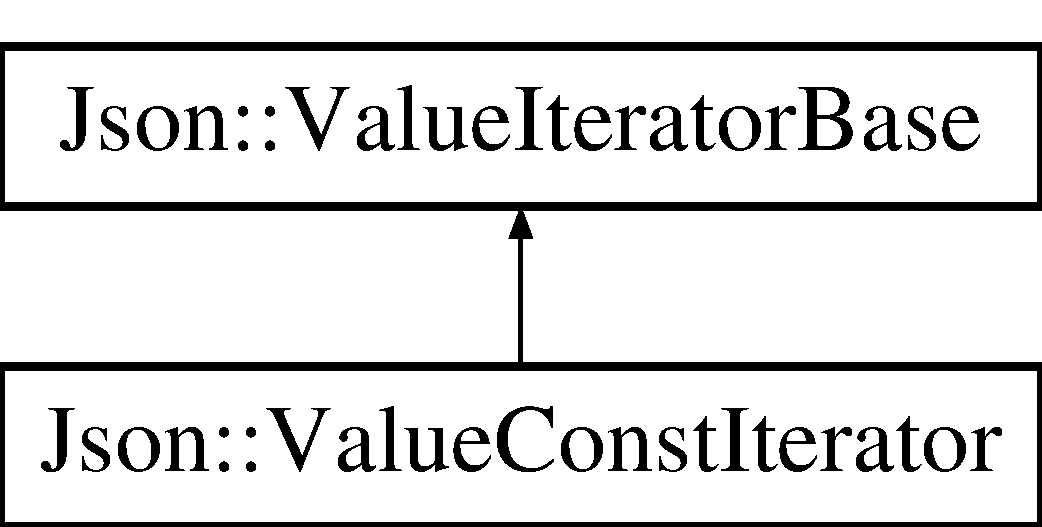
\includegraphics[height=2.000000cm]{class_json_1_1_value_const_iterator}
\end{center}
\end{figure}
\subsection*{Public Types}
\begin{DoxyCompactItemize}
\item 
\hypertarget{class_json_1_1_value_const_iterator_aa5f1707dcef4bfe73e23ddc14dbe760d}{}typedef const \hyperlink{class_json_1_1_value}{Value} {\bfseries value\+\_\+type}\label{class_json_1_1_value_const_iterator_aa5f1707dcef4bfe73e23ddc14dbe760d}

\item 
\hypertarget{class_json_1_1_value_const_iterator_aa9b05c6a37cd352ea1ee6e13b816f709}{}typedef const \hyperlink{class_json_1_1_value}{Value} \& {\bfseries reference}\label{class_json_1_1_value_const_iterator_aa9b05c6a37cd352ea1ee6e13b816f709}

\item 
\hypertarget{class_json_1_1_value_const_iterator_a400136bd8bc09e9fddec0785fa2cff14}{}typedef const \hyperlink{class_json_1_1_value}{Value} $\ast$ {\bfseries pointer}\label{class_json_1_1_value_const_iterator_a400136bd8bc09e9fddec0785fa2cff14}

\item 
\hypertarget{class_json_1_1_value_const_iterator_a0c2e33e7eb5a80dd8709fb28ece83933}{}typedef \hyperlink{class_json_1_1_value_const_iterator}{Value\+Const\+Iterator} {\bfseries Self\+Type}\label{class_json_1_1_value_const_iterator_a0c2e33e7eb5a80dd8709fb28ece83933}

\end{DoxyCompactItemize}
\subsection*{Public Member Functions}
\begin{DoxyCompactItemize}
\item 
\hypertarget{class_json_1_1_value_const_iterator_ad1b1c11f8d7fb22d4d3c231915f2b15b}{}\hyperlink{class_json_1_1_value_iterator_base}{Self\+Type} \& {\bfseries operator=} (const \hyperlink{class_json_1_1_value_iterator_base}{Value\+Iterator\+Base} \&other)\label{class_json_1_1_value_const_iterator_ad1b1c11f8d7fb22d4d3c231915f2b15b}

\item 
\hypertarget{class_json_1_1_value_const_iterator_ab3f0c2edbfc8f7d60645f3d597d05e28}{}\hyperlink{class_json_1_1_value_iterator_base}{Self\+Type} {\bfseries operator++} (int)\label{class_json_1_1_value_const_iterator_ab3f0c2edbfc8f7d60645f3d597d05e28}

\item 
\hypertarget{class_json_1_1_value_const_iterator_a94935961e9331c6f7b907b05ec8df75e}{}\hyperlink{class_json_1_1_value_iterator_base}{Self\+Type} {\bfseries operator-\/-\/} (int)\label{class_json_1_1_value_const_iterator_a94935961e9331c6f7b907b05ec8df75e}

\item 
\hypertarget{class_json_1_1_value_const_iterator_a31415e44e44e56fb2bfda7e8bb784646}{}\hyperlink{class_json_1_1_value_iterator_base}{Self\+Type} \& {\bfseries operator-\/-\/} ()\label{class_json_1_1_value_const_iterator_a31415e44e44e56fb2bfda7e8bb784646}

\item 
\hypertarget{class_json_1_1_value_const_iterator_a2cfe2f7a94a688186efdafb1b181c319}{}\hyperlink{class_json_1_1_value_iterator_base}{Self\+Type} \& {\bfseries operator++} ()\label{class_json_1_1_value_const_iterator_a2cfe2f7a94a688186efdafb1b181c319}

\item 
\hypertarget{class_json_1_1_value_const_iterator_aeb44153d71c61ac9397a84d5ecc244c5}{}\hyperlink{class_json_1_1_value}{reference} {\bfseries operator$\ast$} () const \label{class_json_1_1_value_const_iterator_aeb44153d71c61ac9397a84d5ecc244c5}

\item 
\hypertarget{class_json_1_1_value_const_iterator_ac493d31c8eede8af10b71415fe8e624b}{}\hyperlink{class_json_1_1_value}{pointer} {\bfseries operator-\/$>$} () const \label{class_json_1_1_value_const_iterator_ac493d31c8eede8af10b71415fe8e624b}

\end{DoxyCompactItemize}
\subsection*{Friends}
\begin{DoxyCompactItemize}
\item 
\hypertarget{class_json_1_1_value_const_iterator_aeceedf6e1a7d48a588516ce2b1983d6f}{}class {\bfseries Value}\label{class_json_1_1_value_const_iterator_aeceedf6e1a7d48a588516ce2b1983d6f}

\end{DoxyCompactItemize}
\subsection*{Additional Inherited Members}


\subsection{Detailed Description}
const iterator for object and array value. 



The documentation for this class was generated from the following files\+:\begin{DoxyCompactItemize}
\item 
/home/robin\+\_\+f/\+Programming/\+Git/\+C\+P\+P/\+Love\+Brains/api/lib/\+A\+N\+N\+Library/include/json/json.\+h\item 
/home/robin\+\_\+f/\+Programming/\+Git/\+C\+P\+P/\+Love\+Brains/api/lib/\+A\+N\+N\+Library/src/json/jsoncpp.\+cc\end{DoxyCompactItemize}

\section{Json\+:\+:Value\+Iterator Class Reference}
\label{class_json_1_1_value_iterator}\index{Json\+::\+Value\+Iterator@{Json\+::\+Value\+Iterator}}


Iterator for object and array value.  




{\ttfamily \#include $<$json.\+h$>$}

Inheritance diagram for Json\+:\+:Value\+Iterator\+:\begin{figure}[H]
\begin{center}
\leavevmode
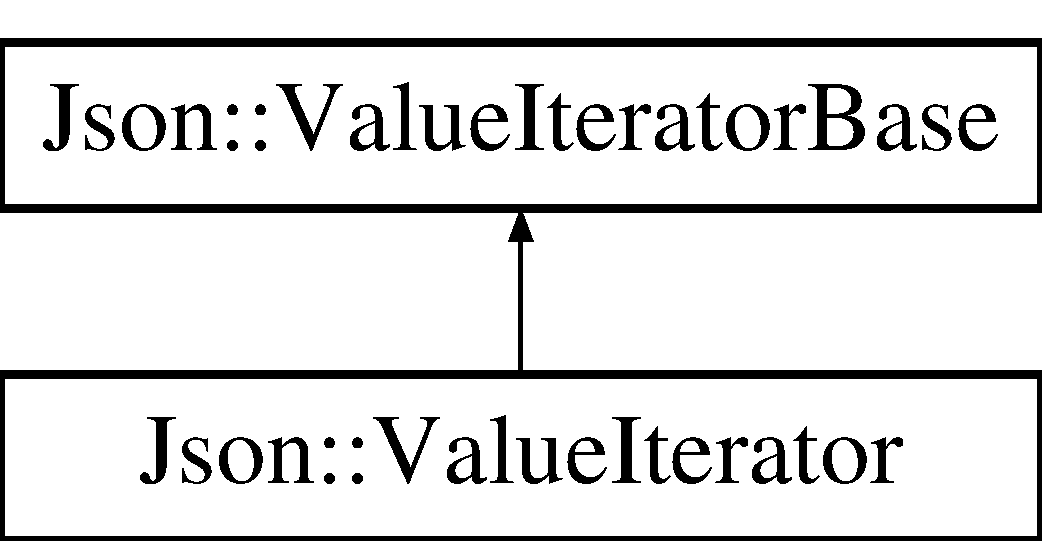
\includegraphics[height=1.818182cm]{class_json_1_1_value_iterator}
\end{center}
\end{figure}
\subsection*{Public Types}
\begin{DoxyCompactItemize}
\item 
typedef {\bf Value} {\bfseries value\+\_\+type}\label{class_json_1_1_value_iterator_a2c5ba7be611f05546530c8a88b2d2e37}

\item 
typedef unsigned int {\bfseries size\+\_\+t}\label{class_json_1_1_value_iterator_a308b8932ffc83eaa9d12dadd5c11a7dd}

\item 
typedef int {\bfseries difference\+\_\+type}\label{class_json_1_1_value_iterator_a2be1a9aa60bbfc8812e9dd1a7f1a8786}

\item 
typedef {\bf Value} \& {\bfseries reference}\label{class_json_1_1_value_iterator_ae87929b4567aa00372cf602c43b57160}

\item 
typedef {\bf Value} $\ast$ {\bfseries pointer}\label{class_json_1_1_value_iterator_acec45feb1ef1f3bf81240157d06d5432}

\item 
typedef {\bf Value\+Iterator} {\bfseries Self\+Type}\label{class_json_1_1_value_iterator_a23357670fdad61792670d86f62db7e16}

\item 
typedef {\bf Value} {\bfseries value\+\_\+type}\label{class_json_1_1_value_iterator_a2c5ba7be611f05546530c8a88b2d2e37}

\item 
typedef unsigned int {\bfseries size\+\_\+t}\label{class_json_1_1_value_iterator_a308b8932ffc83eaa9d12dadd5c11a7dd}

\item 
typedef int {\bfseries difference\+\_\+type}\label{class_json_1_1_value_iterator_a2be1a9aa60bbfc8812e9dd1a7f1a8786}

\item 
typedef {\bf Value} \& {\bfseries reference}\label{class_json_1_1_value_iterator_ae87929b4567aa00372cf602c43b57160}

\item 
typedef {\bf Value} $\ast$ {\bfseries pointer}\label{class_json_1_1_value_iterator_acec45feb1ef1f3bf81240157d06d5432}

\item 
typedef {\bf Value\+Iterator} {\bfseries Self\+Type}\label{class_json_1_1_value_iterator_a23357670fdad61792670d86f62db7e16}

\item 
typedef {\bf Value} {\bfseries value\+\_\+type}\label{class_json_1_1_value_iterator_a2c5ba7be611f05546530c8a88b2d2e37}

\item 
typedef unsigned int {\bfseries size\+\_\+t}\label{class_json_1_1_value_iterator_a308b8932ffc83eaa9d12dadd5c11a7dd}

\item 
typedef int {\bfseries difference\+\_\+type}\label{class_json_1_1_value_iterator_a2be1a9aa60bbfc8812e9dd1a7f1a8786}

\item 
typedef {\bf Value} \& {\bfseries reference}\label{class_json_1_1_value_iterator_ae87929b4567aa00372cf602c43b57160}

\item 
typedef {\bf Value} $\ast$ {\bfseries pointer}\label{class_json_1_1_value_iterator_acec45feb1ef1f3bf81240157d06d5432}

\item 
typedef {\bf Value\+Iterator} {\bfseries Self\+Type}\label{class_json_1_1_value_iterator_a23357670fdad61792670d86f62db7e16}

\item 
typedef {\bf Value} {\bfseries value\+\_\+type}\label{class_json_1_1_value_iterator_a2c5ba7be611f05546530c8a88b2d2e37}

\item 
typedef unsigned int {\bfseries size\+\_\+t}\label{class_json_1_1_value_iterator_a308b8932ffc83eaa9d12dadd5c11a7dd}

\item 
typedef int {\bfseries difference\+\_\+type}\label{class_json_1_1_value_iterator_a2be1a9aa60bbfc8812e9dd1a7f1a8786}

\item 
typedef {\bf Value} \& {\bfseries reference}\label{class_json_1_1_value_iterator_ae87929b4567aa00372cf602c43b57160}

\item 
typedef {\bf Value} $\ast$ {\bfseries pointer}\label{class_json_1_1_value_iterator_acec45feb1ef1f3bf81240157d06d5432}

\item 
typedef {\bf Value\+Iterator} {\bfseries Self\+Type}\label{class_json_1_1_value_iterator_a23357670fdad61792670d86f62db7e16}

\end{DoxyCompactItemize}
\subsection*{Public Member Functions}
\begin{DoxyCompactItemize}
\item 
{\bfseries Value\+Iterator} (const {\bf Value\+Const\+Iterator} \&other)\label{class_json_1_1_value_iterator_aa85aa208670891670392259efa0143bb}

\item 
{\bfseries Value\+Iterator} (const {\bf Value\+Iterator} \&other)\label{class_json_1_1_value_iterator_a7d5e58a9a4a553968acdf3064b39d21c}

\item 
{\bf Self\+Type} \& {\bfseries operator=} (const {\bf Self\+Type} \&other)\label{class_json_1_1_value_iterator_a8e23312b1db874f7e403fd7e76611bdc}

\item 
{\bf Self\+Type} {\bfseries operator++} (int)\label{class_json_1_1_value_iterator_abcf4ddd994a010742cd4a436d65acd08}

\item 
{\bf Self\+Type} {\bfseries operator-\/-\/} (int)\label{class_json_1_1_value_iterator_a06d6a29d96caf6af324a53973159e12b}

\item 
{\bf Self\+Type} \& {\bfseries operator-\/-\/} ()\label{class_json_1_1_value_iterator_a811302a868518a0995a9def955df5720}

\item 
{\bf Self\+Type} \& {\bfseries operator++} ()\label{class_json_1_1_value_iterator_a92146c46f8249e2b2d12869e70cd4cee}

\item 
{\bf reference} {\bfseries operator$\ast$} () const \label{class_json_1_1_value_iterator_aaa5be3457eedf0526a03b8a3b4c7c0a0}

\item 
{\bf pointer} {\bfseries operator-\/$>$} () const \label{class_json_1_1_value_iterator_ad9882e4ce815cef6a504afa113544bfb}

\item 
{\bfseries Value\+Iterator} (const {\bf Value\+Const\+Iterator} \&other)\label{class_json_1_1_value_iterator_aa85aa208670891670392259efa0143bb}

\item 
{\bfseries Value\+Iterator} (const {\bf Value\+Iterator} \&other)\label{class_json_1_1_value_iterator_a7d5e58a9a4a553968acdf3064b39d21c}

\item 
{\bf Self\+Type} \& {\bfseries operator=} (const {\bf Self\+Type} \&other)\label{class_json_1_1_value_iterator_a263912ab48a278202312cfddf636bc71}

\item 
{\bf Self\+Type} {\bfseries operator++} (int)\label{class_json_1_1_value_iterator_abcf4ddd994a010742cd4a436d65acd08}

\item 
{\bf Self\+Type} {\bfseries operator-\/-\/} (int)\label{class_json_1_1_value_iterator_a06d6a29d96caf6af324a53973159e12b}

\item 
{\bf Self\+Type} \& {\bfseries operator-\/-\/} ()\label{class_json_1_1_value_iterator_a811302a868518a0995a9def955df5720}

\item 
{\bf Self\+Type} \& {\bfseries operator++} ()\label{class_json_1_1_value_iterator_a92146c46f8249e2b2d12869e70cd4cee}

\item 
{\bf reference} {\bfseries operator$\ast$} () const \label{class_json_1_1_value_iterator_aaa5be3457eedf0526a03b8a3b4c7c0a0}

\item 
{\bf pointer} {\bfseries operator-\/$>$} () const \label{class_json_1_1_value_iterator_ad9882e4ce815cef6a504afa113544bfb}

\item 
{\bfseries Value\+Iterator} (const {\bf Value\+Const\+Iterator} \&other)\label{class_json_1_1_value_iterator_aa85aa208670891670392259efa0143bb}

\item 
{\bfseries Value\+Iterator} (const {\bf Value\+Iterator} \&other)\label{class_json_1_1_value_iterator_a7d5e58a9a4a553968acdf3064b39d21c}

\item 
{\bf Self\+Type} \& {\bfseries operator=} (const {\bf Self\+Type} \&other)\label{class_json_1_1_value_iterator_a263912ab48a278202312cfddf636bc71}

\item 
{\bf Self\+Type} {\bfseries operator++} (int)\label{class_json_1_1_value_iterator_abcf4ddd994a010742cd4a436d65acd08}

\item 
{\bf Self\+Type} {\bfseries operator-\/-\/} (int)\label{class_json_1_1_value_iterator_a06d6a29d96caf6af324a53973159e12b}

\item 
{\bf Self\+Type} \& {\bfseries operator-\/-\/} ()\label{class_json_1_1_value_iterator_a811302a868518a0995a9def955df5720}

\item 
{\bf Self\+Type} \& {\bfseries operator++} ()\label{class_json_1_1_value_iterator_a92146c46f8249e2b2d12869e70cd4cee}

\item 
{\bf reference} {\bfseries operator$\ast$} () const \label{class_json_1_1_value_iterator_aaa5be3457eedf0526a03b8a3b4c7c0a0}

\item 
{\bf pointer} {\bfseries operator-\/$>$} () const \label{class_json_1_1_value_iterator_ad9882e4ce815cef6a504afa113544bfb}

\item 
{\bfseries Value\+Iterator} (const {\bf Value\+Const\+Iterator} \&other)\label{class_json_1_1_value_iterator_aa85aa208670891670392259efa0143bb}

\item 
{\bfseries Value\+Iterator} (const {\bf Value\+Iterator} \&other)\label{class_json_1_1_value_iterator_a7d5e58a9a4a553968acdf3064b39d21c}

\item 
{\bf Self\+Type} \& {\bfseries operator=} (const {\bf Self\+Type} \&other)\label{class_json_1_1_value_iterator_a263912ab48a278202312cfddf636bc71}

\item 
{\bf Self\+Type} {\bfseries operator++} (int)\label{class_json_1_1_value_iterator_abcf4ddd994a010742cd4a436d65acd08}

\item 
{\bf Self\+Type} {\bfseries operator-\/-\/} (int)\label{class_json_1_1_value_iterator_a06d6a29d96caf6af324a53973159e12b}

\item 
{\bf Self\+Type} \& {\bfseries operator-\/-\/} ()\label{class_json_1_1_value_iterator_a811302a868518a0995a9def955df5720}

\item 
{\bf Self\+Type} \& {\bfseries operator++} ()\label{class_json_1_1_value_iterator_a92146c46f8249e2b2d12869e70cd4cee}

\item 
{\bf reference} {\bfseries operator$\ast$} () const \label{class_json_1_1_value_iterator_aaa5be3457eedf0526a03b8a3b4c7c0a0}

\item 
{\bf pointer} {\bfseries operator-\/$>$} () const \label{class_json_1_1_value_iterator_ad9882e4ce815cef6a504afa113544bfb}

\end{DoxyCompactItemize}
\subsection*{Friends}
\begin{DoxyCompactItemize}
\item 
class {\bfseries Value}\label{class_json_1_1_value_iterator_a896c037a32087c5c20d97e64a1786880}

\end{DoxyCompactItemize}
\subsection*{Additional Inherited Members}


\subsection{Detailed Description}
Iterator for object and array value. 

The documentation for this class was generated from the following files\+:\begin{DoxyCompactItemize}
\item 
api/lib/\+A\+N\+N\+Library/include/json/json.\+h\item 
api/lib/\+A\+N\+N\+Library/src/json/jsoncpp.\+cc\end{DoxyCompactItemize}

\section{Json\+:\+:Value\+Iterator\+Base Class Reference}
\label{class_json_1_1_value_iterator_base}\index{Json\+::\+Value\+Iterator\+Base@{Json\+::\+Value\+Iterator\+Base}}


base class for \doxyref{Value}{p.}{class_json_1_1_value} iterators.  




{\ttfamily \#include $<$json.\+h$>$}

Inheritance diagram for Json\+:\+:Value\+Iterator\+Base\+:\begin{figure}[H]
\begin{center}
\leavevmode
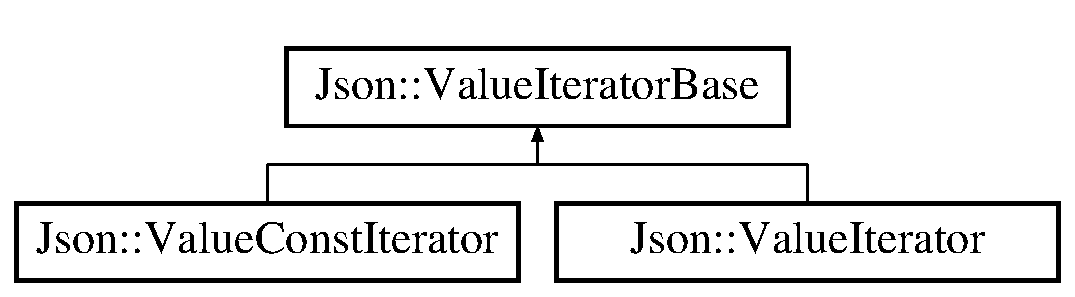
\includegraphics[height=9.000000cm]{class_json_1_1_value_iterator_base}
\end{center}
\end{figure}
\subsection*{Public Types}
\begin{DoxyCompactItemize}
\item 
typedef std\+::bidirectional\+\_\+iterator\+\_\+tag {\bfseries iterator\+\_\+category}\label{class_json_1_1_value_iterator_base_a02fd11a4fbdc0007da1e8bcf5e6b83c3}

\item 
typedef unsigned int {\bfseries size\+\_\+t}\label{class_json_1_1_value_iterator_base_a9d3a3c7ce5cdefe23cb486239cf07bb5}

\item 
typedef int {\bfseries difference\+\_\+type}\label{class_json_1_1_value_iterator_base_a4e44bf8cbd17ec8d6e2c185904a15ebd}

\item 
typedef {\bf Value\+Iterator\+Base} {\bfseries Self\+Type}\label{class_json_1_1_value_iterator_base_a9d2a940d03ea06d20d972f41a89149ee}

\item 
typedef std\+::bidirectional\+\_\+iterator\+\_\+tag {\bfseries iterator\+\_\+category}\label{class_json_1_1_value_iterator_base_a02fd11a4fbdc0007da1e8bcf5e6b83c3}

\item 
typedef unsigned int {\bfseries size\+\_\+t}\label{class_json_1_1_value_iterator_base_a9d3a3c7ce5cdefe23cb486239cf07bb5}

\item 
typedef int {\bfseries difference\+\_\+type}\label{class_json_1_1_value_iterator_base_a4e44bf8cbd17ec8d6e2c185904a15ebd}

\item 
typedef {\bf Value\+Iterator\+Base} {\bfseries Self\+Type}\label{class_json_1_1_value_iterator_base_a9d2a940d03ea06d20d972f41a89149ee}

\item 
typedef std\+::bidirectional\+\_\+iterator\+\_\+tag {\bfseries iterator\+\_\+category}\label{class_json_1_1_value_iterator_base_a02fd11a4fbdc0007da1e8bcf5e6b83c3}

\item 
typedef unsigned int {\bfseries size\+\_\+t}\label{class_json_1_1_value_iterator_base_a9d3a3c7ce5cdefe23cb486239cf07bb5}

\item 
typedef int {\bfseries difference\+\_\+type}\label{class_json_1_1_value_iterator_base_a4e44bf8cbd17ec8d6e2c185904a15ebd}

\item 
typedef {\bf Value\+Iterator\+Base} {\bfseries Self\+Type}\label{class_json_1_1_value_iterator_base_a9d2a940d03ea06d20d972f41a89149ee}

\item 
typedef std\+::bidirectional\+\_\+iterator\+\_\+tag {\bfseries iterator\+\_\+category}\label{class_json_1_1_value_iterator_base_a02fd11a4fbdc0007da1e8bcf5e6b83c3}

\item 
typedef unsigned int {\bfseries size\+\_\+t}\label{class_json_1_1_value_iterator_base_a9d3a3c7ce5cdefe23cb486239cf07bb5}

\item 
typedef int {\bfseries difference\+\_\+type}\label{class_json_1_1_value_iterator_base_a4e44bf8cbd17ec8d6e2c185904a15ebd}

\item 
typedef {\bf Value\+Iterator\+Base} {\bfseries Self\+Type}\label{class_json_1_1_value_iterator_base_a9d2a940d03ea06d20d972f41a89149ee}

\end{DoxyCompactItemize}
\subsection*{Public Member Functions}
\begin{DoxyCompactItemize}
\item 
bool {\bfseries operator==} (const {\bf Self\+Type} \&other) const \label{class_json_1_1_value_iterator_base_afc656672ac28502f640ade32c38c1b56}

\item 
bool {\bfseries operator!=} (const {\bf Self\+Type} \&other) const \label{class_json_1_1_value_iterator_base_a18c2dd42e0bb989ace141bfe9de52792}

\item 
difference\+\_\+type {\bfseries operator-\/} (const {\bf Self\+Type} \&other) const \label{class_json_1_1_value_iterator_base_ab786787fcad68ca5e8745aaf520fa17f}

\item 
{\bf Value} {\bf key} () const 
\item 
U\+Int {\bf index} () const \label{class_json_1_1_value_iterator_base_aa90591f5f7f8d2f06cc4605816b53738}

\begin{DoxyCompactList}\small\item\em Return the index of the referenced \doxyref{Value}{p.}{class_json_1_1_value}, or -\/1 if it is not an array\+Value. \end{DoxyCompactList}\item 
std\+::string {\bf name} () const 
\item 
char const $\ast$ {\bf member\+Name} () const 
\item 
char const $\ast$ {\bf member\+Name} (char const $\ast$$\ast$end) const 
\item 
{\bfseries Value\+Iterator\+Base} (const Value\+::\+Object\+Values\+::iterator \&current)\label{class_json_1_1_value_iterator_base_a640e990e5f03a96fd650122a2906f59d}

\item 
bool {\bfseries operator==} (const {\bf Self\+Type} \&other) const \label{class_json_1_1_value_iterator_base_afc656672ac28502f640ade32c38c1b56}

\item 
bool {\bfseries operator!=} (const {\bf Self\+Type} \&other) const \label{class_json_1_1_value_iterator_base_a18c2dd42e0bb989ace141bfe9de52792}

\item 
difference\+\_\+type {\bfseries operator-\/} (const {\bf Self\+Type} \&other) const \label{class_json_1_1_value_iterator_base_ab786787fcad68ca5e8745aaf520fa17f}

\item 
{\bf Value} {\bf key} () const 
\item 
U\+Int {\bf index} () const \label{class_json_1_1_value_iterator_base_aa90591f5f7f8d2f06cc4605816b53738}

\begin{DoxyCompactList}\small\item\em Return the index of the referenced \doxyref{Value}{p.}{class_json_1_1_value}, or -\/1 if it is not an array\+Value. \end{DoxyCompactList}\item 
std\+::string {\bf name} () const 
\item 
char const $\ast$ {\bf member\+Name} () const 
\item 
char const $\ast$ {\bf member\+Name} (char const $\ast$$\ast$end) const 
\item 
{\bfseries Value\+Iterator\+Base} (const Value\+::\+Object\+Values\+::iterator \&current)\label{class_json_1_1_value_iterator_base_a640e990e5f03a96fd650122a2906f59d}

\item 
bool {\bfseries operator==} (const {\bf Self\+Type} \&other) const \label{class_json_1_1_value_iterator_base_afc656672ac28502f640ade32c38c1b56}

\item 
bool {\bfseries operator!=} (const {\bf Self\+Type} \&other) const \label{class_json_1_1_value_iterator_base_a18c2dd42e0bb989ace141bfe9de52792}

\item 
difference\+\_\+type {\bfseries operator-\/} (const {\bf Self\+Type} \&other) const \label{class_json_1_1_value_iterator_base_ab786787fcad68ca5e8745aaf520fa17f}

\item 
{\bf Value} {\bf key} () const 
\item 
U\+Int {\bf index} () const \label{class_json_1_1_value_iterator_base_aa90591f5f7f8d2f06cc4605816b53738}

\begin{DoxyCompactList}\small\item\em Return the index of the referenced \doxyref{Value}{p.}{class_json_1_1_value}, or -\/1 if it is not an array\+Value. \end{DoxyCompactList}\item 
std\+::string {\bf name} () const 
\item 
char const $\ast$ {\bf member\+Name} () const 
\item 
char const $\ast$ {\bf member\+Name} (char const $\ast$$\ast$end) const 
\item 
{\bfseries Value\+Iterator\+Base} (const Value\+::\+Object\+Values\+::iterator \&current)\label{class_json_1_1_value_iterator_base_a640e990e5f03a96fd650122a2906f59d}

\item 
bool {\bfseries operator==} (const {\bf Self\+Type} \&other) const \label{class_json_1_1_value_iterator_base_afc656672ac28502f640ade32c38c1b56}

\item 
bool {\bfseries operator!=} (const {\bf Self\+Type} \&other) const \label{class_json_1_1_value_iterator_base_a18c2dd42e0bb989ace141bfe9de52792}

\item 
difference\+\_\+type {\bfseries operator-\/} (const {\bf Self\+Type} \&other) const \label{class_json_1_1_value_iterator_base_ab786787fcad68ca5e8745aaf520fa17f}

\item 
{\bf Value} {\bf key} () const 
\item 
U\+Int {\bf index} () const \label{class_json_1_1_value_iterator_base_aa90591f5f7f8d2f06cc4605816b53738}

\begin{DoxyCompactList}\small\item\em Return the index of the referenced \doxyref{Value}{p.}{class_json_1_1_value}, or -\/1 if it is not an array\+Value. \end{DoxyCompactList}\item 
std\+::string {\bf name} () const 
\item 
char const $\ast$ {\bf member\+Name} () const 
\item 
char const $\ast$ {\bf member\+Name} (char const $\ast$$\ast$end) const 
\item 
{\bfseries Value\+Iterator\+Base} (const Value\+::\+Object\+Values\+::iterator \&current)\label{class_json_1_1_value_iterator_base_a640e990e5f03a96fd650122a2906f59d}

\end{DoxyCompactItemize}
\subsection*{Protected Member Functions}
\begin{DoxyCompactItemize}
\item 
{\bf Value} \& {\bfseries deref} () const \label{class_json_1_1_value_iterator_base_a40a20c65abc423a26e3aae68d9a0525c}

\item 
void {\bfseries increment} ()\label{class_json_1_1_value_iterator_base_afe58f9534e1fd2033419fd9fe244551e}

\item 
void {\bfseries decrement} ()\label{class_json_1_1_value_iterator_base_affc8cf5ff54a9f432cc693362c153fa6}

\item 
difference\+\_\+type {\bfseries compute\+Distance} (const {\bf Self\+Type} \&other) const \label{class_json_1_1_value_iterator_base_ad6c553b249e89e3dc9933e100ccbe064}

\item 
bool {\bfseries is\+Equal} (const {\bf Self\+Type} \&other) const \label{class_json_1_1_value_iterator_base_a21820d6ee564e541bd118b21e4741962}

\item 
void {\bfseries copy} (const {\bf Self\+Type} \&other)\label{class_json_1_1_value_iterator_base_a496e6aba44808433ec5858c178be5719}

\item 
{\bf Value} \& {\bfseries deref} () const \label{class_json_1_1_value_iterator_base_ae675a893b0ad7959e4f5e5aa328b5998}

\item 
void {\bfseries increment} ()\label{class_json_1_1_value_iterator_base_afe58f9534e1fd2033419fd9fe244551e}

\item 
void {\bfseries decrement} ()\label{class_json_1_1_value_iterator_base_affc8cf5ff54a9f432cc693362c153fa6}

\item 
difference\+\_\+type {\bfseries compute\+Distance} (const {\bf Self\+Type} \&other) const \label{class_json_1_1_value_iterator_base_ac52902f3f8369c195a1c2a147dad519a}

\item 
bool {\bfseries is\+Equal} (const {\bf Self\+Type} \&other) const \label{class_json_1_1_value_iterator_base_a21820d6ee564e541bd118b21e4741962}

\item 
void {\bfseries copy} (const {\bf Self\+Type} \&other)\label{class_json_1_1_value_iterator_base_a496e6aba44808433ec5858c178be5719}

\item 
{\bf Value} \& {\bfseries deref} () const \label{class_json_1_1_value_iterator_base_ae675a893b0ad7959e4f5e5aa328b5998}

\item 
void {\bfseries increment} ()\label{class_json_1_1_value_iterator_base_afe58f9534e1fd2033419fd9fe244551e}

\item 
void {\bfseries decrement} ()\label{class_json_1_1_value_iterator_base_affc8cf5ff54a9f432cc693362c153fa6}

\item 
difference\+\_\+type {\bfseries compute\+Distance} (const {\bf Self\+Type} \&other) const \label{class_json_1_1_value_iterator_base_ac52902f3f8369c195a1c2a147dad519a}

\item 
bool {\bfseries is\+Equal} (const {\bf Self\+Type} \&other) const \label{class_json_1_1_value_iterator_base_a21820d6ee564e541bd118b21e4741962}

\item 
void {\bfseries copy} (const {\bf Self\+Type} \&other)\label{class_json_1_1_value_iterator_base_a496e6aba44808433ec5858c178be5719}

\item 
{\bf Value} \& {\bfseries deref} () const \label{class_json_1_1_value_iterator_base_ae675a893b0ad7959e4f5e5aa328b5998}

\item 
void {\bfseries increment} ()\label{class_json_1_1_value_iterator_base_afe58f9534e1fd2033419fd9fe244551e}

\item 
void {\bfseries decrement} ()\label{class_json_1_1_value_iterator_base_affc8cf5ff54a9f432cc693362c153fa6}

\item 
difference\+\_\+type {\bfseries compute\+Distance} (const {\bf Self\+Type} \&other) const \label{class_json_1_1_value_iterator_base_ac52902f3f8369c195a1c2a147dad519a}

\item 
bool {\bfseries is\+Equal} (const {\bf Self\+Type} \&other) const \label{class_json_1_1_value_iterator_base_a21820d6ee564e541bd118b21e4741962}

\item 
void {\bfseries copy} (const {\bf Self\+Type} \&other)\label{class_json_1_1_value_iterator_base_a496e6aba44808433ec5858c178be5719}

\end{DoxyCompactItemize}


\subsection{Detailed Description}
base class for \doxyref{Value}{p.}{class_json_1_1_value} iterators. 



\subsection{Member Function Documentation}
\index{Json\+::\+Value\+Iterator\+Base@{Json\+::\+Value\+Iterator\+Base}!key@{key}}
\index{key@{key}!Json\+::\+Value\+Iterator\+Base@{Json\+::\+Value\+Iterator\+Base}}
\subsubsection[{key() const }]{\setlength{\rightskip}{0pt plus 5cm}{\bf Value} Json\+::\+Value\+Iterator\+Base\+::key (
\begin{DoxyParamCaption}
{}
\end{DoxyParamCaption}
) const}\label{class_json_1_1_value_iterator_base_aa2ff5e79fc96acd4c3cd288e92614fc7}
Return either the index or the member name of the referenced value as a \doxyref{Value}{p.}{class_json_1_1_value}. \index{Json\+::\+Value\+Iterator\+Base@{Json\+::\+Value\+Iterator\+Base}!key@{key}}
\index{key@{key}!Json\+::\+Value\+Iterator\+Base@{Json\+::\+Value\+Iterator\+Base}}
\subsubsection[{key() const }]{\setlength{\rightskip}{0pt plus 5cm}{\bf Value} Json\+::\+Value\+Iterator\+Base\+::key (
\begin{DoxyParamCaption}
{}
\end{DoxyParamCaption}
) const}\label{class_json_1_1_value_iterator_base_aa2ff5e79fc96acd4c3cd288e92614fc7}
Return either the index or the member name of the referenced value as a \doxyref{Value}{p.}{class_json_1_1_value}. \index{Json\+::\+Value\+Iterator\+Base@{Json\+::\+Value\+Iterator\+Base}!key@{key}}
\index{key@{key}!Json\+::\+Value\+Iterator\+Base@{Json\+::\+Value\+Iterator\+Base}}
\subsubsection[{key() const }]{\setlength{\rightskip}{0pt plus 5cm}{\bf Value} Json\+::\+Value\+Iterator\+Base\+::key (
\begin{DoxyParamCaption}
{}
\end{DoxyParamCaption}
) const}\label{class_json_1_1_value_iterator_base_aa2ff5e79fc96acd4c3cd288e92614fc7}
Return either the index or the member name of the referenced value as a \doxyref{Value}{p.}{class_json_1_1_value}. \index{Json\+::\+Value\+Iterator\+Base@{Json\+::\+Value\+Iterator\+Base}!key@{key}}
\index{key@{key}!Json\+::\+Value\+Iterator\+Base@{Json\+::\+Value\+Iterator\+Base}}
\subsubsection[{key() const }]{\setlength{\rightskip}{0pt plus 5cm}{\bf Value} Json\+::\+Value\+Iterator\+Base\+::key (
\begin{DoxyParamCaption}
{}
\end{DoxyParamCaption}
) const}\label{class_json_1_1_value_iterator_base_aa2ff5e79fc96acd4c3cd288e92614fc7}
Return either the index or the member name of the referenced value as a \doxyref{Value}{p.}{class_json_1_1_value}. \index{Json\+::\+Value\+Iterator\+Base@{Json\+::\+Value\+Iterator\+Base}!member\+Name@{member\+Name}}
\index{member\+Name@{member\+Name}!Json\+::\+Value\+Iterator\+Base@{Json\+::\+Value\+Iterator\+Base}}
\subsubsection[{member\+Name() const }]{\setlength{\rightskip}{0pt plus 5cm}char const$\ast$ Json\+::\+Value\+Iterator\+Base\+::member\+Name (
\begin{DoxyParamCaption}
{}
\end{DoxyParamCaption}
) const}\label{class_json_1_1_value_iterator_base_a9a59b5f04e3ee62b851906bb0925138d}
Return the member name of the referenced \doxyref{Value}{p.}{class_json_1_1_value}. \char`\"{}\char`\"{} if it is not an object\+Value. \begin{DoxyRefDesc}{Deprecated}
\item[{\bf Deprecated}]This cannot be used for U\+T\+F-\/8 strings, since there can be embedded nulls. \end{DoxyRefDesc}
\index{Json\+::\+Value\+Iterator\+Base@{Json\+::\+Value\+Iterator\+Base}!member\+Name@{member\+Name}}
\index{member\+Name@{member\+Name}!Json\+::\+Value\+Iterator\+Base@{Json\+::\+Value\+Iterator\+Base}}
\subsubsection[{member\+Name() const }]{\setlength{\rightskip}{0pt plus 5cm}char const$\ast$ Json\+::\+Value\+Iterator\+Base\+::member\+Name (
\begin{DoxyParamCaption}
{}
\end{DoxyParamCaption}
) const}\label{class_json_1_1_value_iterator_base_a9a59b5f04e3ee62b851906bb0925138d}
Return the member name of the referenced \doxyref{Value}{p.}{class_json_1_1_value}. \char`\"{}\char`\"{} if it is not an object\+Value. \begin{DoxyRefDesc}{Deprecated}
\item[{\bf Deprecated}]This cannot be used for U\+T\+F-\/8 strings, since there can be embedded nulls. \end{DoxyRefDesc}
\index{Json\+::\+Value\+Iterator\+Base@{Json\+::\+Value\+Iterator\+Base}!member\+Name@{member\+Name}}
\index{member\+Name@{member\+Name}!Json\+::\+Value\+Iterator\+Base@{Json\+::\+Value\+Iterator\+Base}}
\subsubsection[{member\+Name() const }]{\setlength{\rightskip}{0pt plus 5cm}char const$\ast$ Json\+::\+Value\+Iterator\+Base\+::member\+Name (
\begin{DoxyParamCaption}
{}
\end{DoxyParamCaption}
) const}\label{class_json_1_1_value_iterator_base_a9a59b5f04e3ee62b851906bb0925138d}
Return the member name of the referenced \doxyref{Value}{p.}{class_json_1_1_value}. \char`\"{}\char`\"{} if it is not an object\+Value. \begin{DoxyRefDesc}{Deprecated}
\item[{\bf Deprecated}]This cannot be used for U\+T\+F-\/8 strings, since there can be embedded nulls. \end{DoxyRefDesc}
\index{Json\+::\+Value\+Iterator\+Base@{Json\+::\+Value\+Iterator\+Base}!member\+Name@{member\+Name}}
\index{member\+Name@{member\+Name}!Json\+::\+Value\+Iterator\+Base@{Json\+::\+Value\+Iterator\+Base}}
\subsubsection[{member\+Name() const }]{\setlength{\rightskip}{0pt plus 5cm}char const $\ast$ Json\+::\+Value\+Iterator\+Base\+::member\+Name (
\begin{DoxyParamCaption}
{}
\end{DoxyParamCaption}
) const}\label{class_json_1_1_value_iterator_base_ac3aa3870761342e47c6486d81f643c6c}
Return the member name of the referenced \doxyref{Value}{p.}{class_json_1_1_value}. \char`\"{}\char`\"{} if it is not an object\+Value. \begin{DoxyRefDesc}{Deprecated}
\item[{\bf Deprecated}]This cannot be used for U\+T\+F-\/8 strings, since there can be embedded nulls. \end{DoxyRefDesc}
\index{Json\+::\+Value\+Iterator\+Base@{Json\+::\+Value\+Iterator\+Base}!member\+Name@{member\+Name}}
\index{member\+Name@{member\+Name}!Json\+::\+Value\+Iterator\+Base@{Json\+::\+Value\+Iterator\+Base}}
\subsubsection[{member\+Name(char const $\ast$$\ast$end) const }]{\setlength{\rightskip}{0pt plus 5cm}char const $\ast$ Json\+::\+Value\+Iterator\+Base\+::member\+Name (
\begin{DoxyParamCaption}
\item[{char const $\ast$$\ast$}]{end}
\end{DoxyParamCaption}
) const}\label{class_json_1_1_value_iterator_base_a543d4e73e3d2d121bc287b24231386c3}
Return the member name of the referenced \doxyref{Value}{p.}{class_json_1_1_value}, or N\+U\+L\+L if it is not an object\+Value. \begin{DoxyNote}{Note}
Better version than \doxyref{member\+Name()}{p.}{class_json_1_1_value_iterator_base_ac3aa3870761342e47c6486d81f643c6c}. Allows embedded nulls. 
\end{DoxyNote}
\index{Json\+::\+Value\+Iterator\+Base@{Json\+::\+Value\+Iterator\+Base}!member\+Name@{member\+Name}}
\index{member\+Name@{member\+Name}!Json\+::\+Value\+Iterator\+Base@{Json\+::\+Value\+Iterator\+Base}}
\subsubsection[{member\+Name(char const $\ast$$\ast$end) const }]{\setlength{\rightskip}{0pt plus 5cm}char const$\ast$ Json\+::\+Value\+Iterator\+Base\+::member\+Name (
\begin{DoxyParamCaption}
\item[{char const $\ast$$\ast$}]{end}
\end{DoxyParamCaption}
) const}\label{class_json_1_1_value_iterator_base_a5922f54bcdf3fb33f38d948de25845f9}
Return the member name of the referenced \doxyref{Value}{p.}{class_json_1_1_value}, or N\+U\+L\+L if it is not an object\+Value. \begin{DoxyNote}{Note}
Better version than \doxyref{member\+Name()}{p.}{class_json_1_1_value_iterator_base_ac3aa3870761342e47c6486d81f643c6c}. Allows embedded nulls. 
\end{DoxyNote}
\index{Json\+::\+Value\+Iterator\+Base@{Json\+::\+Value\+Iterator\+Base}!member\+Name@{member\+Name}}
\index{member\+Name@{member\+Name}!Json\+::\+Value\+Iterator\+Base@{Json\+::\+Value\+Iterator\+Base}}
\subsubsection[{member\+Name(char const $\ast$$\ast$end) const }]{\setlength{\rightskip}{0pt plus 5cm}char const$\ast$ Json\+::\+Value\+Iterator\+Base\+::member\+Name (
\begin{DoxyParamCaption}
\item[{char const $\ast$$\ast$}]{end}
\end{DoxyParamCaption}
) const}\label{class_json_1_1_value_iterator_base_a5922f54bcdf3fb33f38d948de25845f9}
Return the member name of the referenced \doxyref{Value}{p.}{class_json_1_1_value}, or N\+U\+L\+L if it is not an object\+Value. \begin{DoxyNote}{Note}
Better version than \doxyref{member\+Name()}{p.}{class_json_1_1_value_iterator_base_ac3aa3870761342e47c6486d81f643c6c}. Allows embedded nulls. 
\end{DoxyNote}
\index{Json\+::\+Value\+Iterator\+Base@{Json\+::\+Value\+Iterator\+Base}!member\+Name@{member\+Name}}
\index{member\+Name@{member\+Name}!Json\+::\+Value\+Iterator\+Base@{Json\+::\+Value\+Iterator\+Base}}
\subsubsection[{member\+Name(char const $\ast$$\ast$end) const }]{\setlength{\rightskip}{0pt plus 5cm}char const$\ast$ Json\+::\+Value\+Iterator\+Base\+::member\+Name (
\begin{DoxyParamCaption}
\item[{char const $\ast$$\ast$}]{end}
\end{DoxyParamCaption}
) const}\label{class_json_1_1_value_iterator_base_a5922f54bcdf3fb33f38d948de25845f9}
Return the member name of the referenced \doxyref{Value}{p.}{class_json_1_1_value}, or N\+U\+L\+L if it is not an object\+Value. \begin{DoxyNote}{Note}
Better version than \doxyref{member\+Name()}{p.}{class_json_1_1_value_iterator_base_ac3aa3870761342e47c6486d81f643c6c}. Allows embedded nulls. 
\end{DoxyNote}
\index{Json\+::\+Value\+Iterator\+Base@{Json\+::\+Value\+Iterator\+Base}!name@{name}}
\index{name@{name}!Json\+::\+Value\+Iterator\+Base@{Json\+::\+Value\+Iterator\+Base}}
\subsubsection[{name() const }]{\setlength{\rightskip}{0pt plus 5cm}std\+::string Json\+::\+Value\+Iterator\+Base\+::name (
\begin{DoxyParamCaption}
{}
\end{DoxyParamCaption}
) const}\label{class_json_1_1_value_iterator_base_a46a67081a5ef8d83f25ec15035403ce0}
Return the member name of the referenced \doxyref{Value}{p.}{class_json_1_1_value}, or \char`\"{}\char`\"{} if it is not an object\+Value. \begin{DoxyNote}{Note}
Avoid {\ttfamily c\+\_\+str()} on result, as embedded zeroes are possible. 
\end{DoxyNote}
\index{Json\+::\+Value\+Iterator\+Base@{Json\+::\+Value\+Iterator\+Base}!name@{name}}
\index{name@{name}!Json\+::\+Value\+Iterator\+Base@{Json\+::\+Value\+Iterator\+Base}}
\subsubsection[{name() const }]{\setlength{\rightskip}{0pt plus 5cm}std\+::string Json\+::\+Value\+Iterator\+Base\+::name (
\begin{DoxyParamCaption}
{}
\end{DoxyParamCaption}
) const}\label{class_json_1_1_value_iterator_base_a46a67081a5ef8d83f25ec15035403ce0}
Return the member name of the referenced \doxyref{Value}{p.}{class_json_1_1_value}, or \char`\"{}\char`\"{} if it is not an object\+Value. \begin{DoxyNote}{Note}
Avoid {\ttfamily c\+\_\+str()} on result, as embedded zeroes are possible. 
\end{DoxyNote}
\index{Json\+::\+Value\+Iterator\+Base@{Json\+::\+Value\+Iterator\+Base}!name@{name}}
\index{name@{name}!Json\+::\+Value\+Iterator\+Base@{Json\+::\+Value\+Iterator\+Base}}
\subsubsection[{name() const }]{\setlength{\rightskip}{0pt plus 5cm}std\+::string Json\+::\+Value\+Iterator\+Base\+::name (
\begin{DoxyParamCaption}
{}
\end{DoxyParamCaption}
) const}\label{class_json_1_1_value_iterator_base_a46a67081a5ef8d83f25ec15035403ce0}
Return the member name of the referenced \doxyref{Value}{p.}{class_json_1_1_value}, or \char`\"{}\char`\"{} if it is not an object\+Value. \begin{DoxyNote}{Note}
Avoid {\ttfamily c\+\_\+str()} on result, as embedded zeroes are possible. 
\end{DoxyNote}
\index{Json\+::\+Value\+Iterator\+Base@{Json\+::\+Value\+Iterator\+Base}!name@{name}}
\index{name@{name}!Json\+::\+Value\+Iterator\+Base@{Json\+::\+Value\+Iterator\+Base}}
\subsubsection[{name() const }]{\setlength{\rightskip}{0pt plus 5cm}std\+::string Json\+::\+Value\+Iterator\+Base\+::name (
\begin{DoxyParamCaption}
{}
\end{DoxyParamCaption}
) const}\label{class_json_1_1_value_iterator_base_a46a67081a5ef8d83f25ec15035403ce0}
Return the member name of the referenced \doxyref{Value}{p.}{class_json_1_1_value}, or \char`\"{}\char`\"{} if it is not an object\+Value. \begin{DoxyNote}{Note}
Avoid {\ttfamily c\+\_\+str()} on result, as embedded zeroes are possible. 
\end{DoxyNote}


The documentation for this class was generated from the following files\+:\begin{DoxyCompactItemize}
\item 
/home/robin\+\_\+f/\+Programming/\+Git/\+C\+P\+P/\+Love\+Brains/api/lib/\+A\+N\+N\+Library/include/json/json.\+h\item 
/home/robin\+\_\+f/\+Programming/\+Git/\+C\+P\+P/\+Love\+Brains/api/lib/\+A\+N\+N\+Library/src/json/jsoncpp.\+cc\end{DoxyCompactItemize}

\hypertarget{class_json_1_1_writer}{}\section{Json\+:\+:Writer Class Reference}
\label{class_json_1_1_writer}\index{Json\+::\+Writer@{Json\+::\+Writer}}


Abstract class for writers.  




{\ttfamily \#include $<$json.\+h$>$}

Inheritance diagram for Json\+:\+:Writer\+:\begin{figure}[H]
\begin{center}
\leavevmode
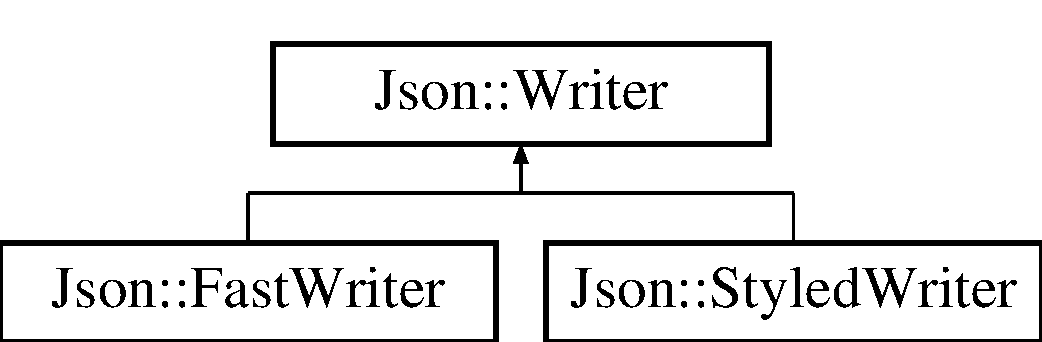
\includegraphics[height=2.000000cm]{class_json_1_1_writer}
\end{center}
\end{figure}
\subsection*{Public Member Functions}
\begin{DoxyCompactItemize}
\item 
\hypertarget{class_json_1_1_writer_a7b2273a4ffd6f32b369ac8a53b7b5a0d}{}virtual std\+::string {\bfseries write} (const \hyperlink{class_json_1_1_value}{Value} \&root)=0\label{class_json_1_1_writer_a7b2273a4ffd6f32b369ac8a53b7b5a0d}

\end{DoxyCompactItemize}


\subsection{Detailed Description}
Abstract class for writers. 

\begin{DoxyRefDesc}{Deprecated}
\item[\hyperlink{deprecated__deprecated000007}{Deprecated}]Use \hyperlink{class_json_1_1_stream_writer}{Stream\+Writer}. (And really, this is an implementation detail.) \end{DoxyRefDesc}


The documentation for this class was generated from the following files\+:\begin{DoxyCompactItemize}
\item 
/home/robin\+\_\+f/\+Programming/\+Git/\+C\+P\+P/\+Love\+Brains/api/lib/\+A\+N\+N\+Library/include/json/json.\+h\item 
/home/robin\+\_\+f/\+Programming/\+Git/\+C\+P\+P/\+Love\+Brains/api/lib/\+A\+N\+N\+Library/src/json/jsoncpp.\+cc\end{DoxyCompactItemize}

%--- End generated contents ---

% Index
\backmatter
\newpage
\phantomsection
\clearemptydoublepage
\addcontentsline{toc}{chapter}{Index}
\printindex

\end{document}
